\RequirePackage{setspace}

\documentclass[
	% -- opções da classe memoir --
	12pt,				% tamanho da fonte
	openright,			% capítulos começam em pág ímpar (insere página vazia caso preciso)
	oneside,			% para impressão em recto e verso. Oposto a oneside
	a4paper,			% tamanho do papel. 
	% -- opções da classe abntex2 --
	chapter=TITLE,		% títulos de capítulos convertidos em letras maiúsculas
	%section=TITLE,		% títulos de seções convertidos em letras maiúsculas
	%subsection=TITLE,	% títulos de subseções convertidos em letras maiúsculas
	%subsubsection=TITLE,% títulos de subsubseções convertidos em letras maiúsculas
	% -- opções do pacote babel --
	english,			% idioma adicional para hifenização
	french,				% idioma adicional para hifenização
	spanish,			% idioma adicional para hifenização
	brazil				% o último idioma é o principal do documento
	]{abntex2}

\linespread{4}	
% ---
% Pacotes básicos 
% ---


\usepackage[alf,abnt-etal-cite=3,abnt-etal-list=0]{abntex2cite}
\usepackage[T1]{fontenc}		% Selecao de codigos de fonte.
\usepackage[utf8]{inputenc}		% Codificacao do documento (conversão automática dos acentos)
\usepackage{lastpage}			% Usado pela Ficha catalográfica
\usepackage{indentfirst}		% Indenta o primeiro parágrafo de cada seção.
\usepackage{color}			% Controle das cores
\usepackage{graphicx}			% Inclusão de gráficos
\usepackage{microtype} 			% Para melhorias de justificação
\usepackage{todonotes}			% Notas para a revisão
\usepackage{enumitem}
\usepackage{textcase}
\usepackage{soul}
\usepackage{soulutf8}

% graficos em 2 colunas
\usepackage{graphicx, multicol}
%equações com aligned
\usepackage{amssymb}
\usepackage{amsthm}
\usepackage{amsfonts}
\usepackage{amsmath}
\usepackage{setspace} 
\usepackage{tikz}
\usetikzlibrary{shapes,arrows,chains,positioning}
\DeclareMathOperator{\atantwo}{atan2}
\DeclareMathOperator{\arctantwo}{arctan2}
\usepackage{hyperref}
\usepackage{multirow}
\usepackage{color, colortbl}
%\usepackage[table]{xcolor}
\definecolor{lightgray}{gray}{0.9}
\usepackage{placeins}
\usepackage{array}

% – inicio codigo fonte 
\usepackage{listings}
\usepackage{xcolor}
\renewcommand{\lstlistingname}{Código-fonte}% Listing -> Códigos
\renewcommand{\lstlistlistingname}{List of \lstlistingname s}% Lista de Códigos
\colorlet{punct}{red!60!black}
\definecolor{background}{HTML}{EEEEEE}
\definecolor{delim}{RGB}{20,105,176}
\colorlet{numb}{magenta!60!black}
\lstdefinelanguage{json}{
    basicstyle=\normalfont\ttfamily,
    numbers=left,
    numberstyle=\scriptsize,
    stepnumber=1,
    numbersep=8pt,
    showstringspaces=false,
    breaklines=true,
    frame=lines,
    backgroundcolor=\color{background},
    literate=
     *{0}{{{\color{numb}0}}}{1}
      {1}{{{\color{numb}1}}}{1}
      {2}{{{\color{numb}2}}}{1}
      {3}{{{\color{numb}3}}}{1}
      {4}{{{\color{numb}4}}}{1}
      {5}{{{\color{numb}5}}}{1}
      {6}{{{\color{numb}6}}}{1}
      {7}{{{\color{numb}7}}}{1}
      {8}{{{\color{numb}8}}}{1}
      {9}{{{\color{numb}9}}}{1}
      {:}{{{\color{punct}{:}}}}{1}
      {,}{{{\color{punct}{,}}}}{1}
      {\{}{{{\color{delim}{\{}}}}{1}
      {\}}{{{\color{delim}{\}}}}}{1}
      {[}{{{\color{delim}{[}}}}{1}
      {]}{{{\color{delim}{]}}}}{1},
}
% – fim codigo fonte

\usepackage{booktabs}

\usepackage{environ}
\makeatletter
\newsavebox{\measure@tikzpicture}
\NewEnviron{scaletikzpicturetowidth}[1]{%
  \def\tikz@width{#1}%
  \def\tikzscale{1}\begin{lrbox}{\measure@tikzpicture}%
  \BODY
  \end{lrbox}%
  \pgfmathparse{#1/\wd\measure@tikzpicture}%
  \edef\tikzscale{\pgfmathresult}%
  \BODY
}
\makeatother


\usepackage{nomencl}

\usepackage{setspace}
\usepackage{printlen}
\usepackage[final]{pdfpages}

\makeindex
\makenomenclature

%\DisemulatePackage{setspace}
\usepackage{setspace}


% ---
		
% ---
% Pacotes adicionais, usados apenas no âmbito do Modelo Canônico do abnteX2
% ---

\usepackage{customizacao}
% ---

% ---
% Pacotes de citações
% ---
\usepackage[brazilian,hyperpageref]{backref}	 % Paginas com as citações na bibl
\usepackage[alf]{abntex2cite}	% Citações padrão ABNT

% --- 
% CONFIGURAÇÕES DE PACOTES
% --- 

%  \usepackage{pslatex}
\usepackage{lmodern}			% Usa a fonte Latin Modern
% \usepackage{txfonts}
% \renewcommand{\familydefault}{\rmdefault}
\renewcommand{\ABNTEXchapterfont}{\bfseries \rmfamily}
%\renewcommand{\ABNTEXchapterfont}{\bfseries \sffamily}
%\renewcommand{\ABNTEXchapterfont}{\fontseries{b}\selectfont}
\renewcommand{\ABNTEXchapterfontsize}{\normalsize}
\renewcommand{\ABNTEXpartfontsize}{\normalsize}
\renewcommand{\ABNTEXsectionfontsize}{\normalsize}
\renewcommand{\ABNTEXsubsectionfontsize}{\normalsize}
\setlength\afterchapskip{\lineskip}
\setlength\beforechapskip{\lineskip}

% % ---
% Configurações do pacote backref
% Usado sem a opção hyperpageref de backref
% \renewcommand{\backrefpagesname}{Citado na(s) página(s):~}
% % Texto padrão antes do número das páginas
% \renewcommand{\backref}{}
% % Define os textos da citação
% \renewcommand*{\backrefalt}[4]{
% 	\ifcase #1 %
% 		Nenhuma citação no texto.%
% 	\or
% 		Citado na página #2.%
% 	\else
% 		Citado #1 vezes nas páginas #2.%
% 	\fi}
	
%  ---
\newcommand*\elide{\textup{[\,\ldots] }}

%%criar um novo estilo de cabeçalhos e rodapés
\makepagestyle{meuestilo}
  %%cabeçalhos
  \makeevenhead{meuestilo} %%pagina par
     {}
     {}
     {\normalsize\thepage}
  \makeoddhead{meuestilo} %%pagina ímpar ou com oneside
     {}
     {}
     {\normalsize\thepage}
  %\makeheadrule{meuestilo}{\textwidth}{\normalrulethickness} %linha
  %% rodapé
  \makeevenfoot{meuestilo}
     {}
     {}
     {} 
  \makeoddfoot{meuestilo} %%pagina ímpar ou com oneside
     {}
     {}
     {}


% ---
% Informações de dados para CAPA e FOLHA DE ROSTO
% ---

\titulo{Segmentação automática de rins e tumores renais em imagens de tomografia computadorizada baseada em aprendizado profundo 2.5D}
%\titulo{Segmentação automática de rins e tumores renais em imagens de tomografia computadorizada usando os modelos Dual Path DeepLabv3+ e ResUNet baseados em abordagem 2.5D}
\autor{LUANA BATISTA DA CRUZ}
\local{SÃO LUÍS - MA}
\data{2022}
\orientador[Orientador:]{Prof. Dr. Aristófanes Corrêa Silva}
\coorientador[Coorientador:]{Prof. Dr. João Dallyson Sousa de Almeida}


\instituicao{%
  UNIVERSIDADE FEDERAL DO MARANHÃO - UFMA
  \par
  CENTRO DE CIÊNCIAS EXATAS E TECNOLOGIA
  \par
  DOUTORADO EM CIÊNCIA DA COMPUTAÇÃO - ASSOCIAÇÃO UFMA/UFPI}
\tipotrabalho{Tese de Doutorado}
% O preambulo deve conter o tipo do trabalho, o objetivo, 
% o nome da instituição e a área de concentração 
\preambulo{Tese apresentada ao Curso de Doutorado em Ciência da Computação - Associação UFMA/UFPI como parte dos requisitos necessários para obtenção do grau de Doutora em Ciência da Computação.
\newline \newline
%Área de concentração: Ciência da Computação.
}
%\preambulo{Versão preliminar de Dissertação de Mestrado apresentada ao Programa de Pós-Graduação em Políticas Públicas para exame de qualificação.}
% ---

% ---
% Configurações de aparência do PDF final

% alterando o aspecto da cor azul
\definecolor{blue}{RGB}{41,5,195}

% informações do PDF
\makeatletter
\hypersetup{
     	%pagebackref=true,
	pdftitle={\@title}, 
	pdfauthor={\@author},
    	pdfsubject={\imprimirpreambulo},
	pdfcreator={PDFLaTeX},
	pdfkeywords={abnt}{latex}{abntex}{abntex2}{trabalho acadêmico; dissertação; mestrado}, 
	colorlinks=true,       		% false: boxed links; true: colored links
    	linkcolor=black,          	% color of internal links
    	citecolor=black,        		% color of links to bibliography
    	filecolor=black,      		% color of file links
	urlcolor=black,
	bookmarksdepth=4
}
\makeatother
% --- 

% --- 
% Espaçamentos entre linhas e parágrafos 
% --- 

% O tamanho do parágrafo é dado por:
\setlength{\parindent}{1.5cm}

% Controle do espaçamento entre um parágrafo e outro:
%\setlength{\parskip}{0.2cm}  % tente também \onelineskip
%\setlength{\parskip}{\onelineskip}  % tente também \onelineskip
% ---
% compila o indice
% ---
\makeindex
% ---

\renewenvironment{quote}%
  {\list{}{\singlespacing\small\leftmargin=4cm\rightmargin=0in\parskip=-0.2cm}\item[]{\parskip=0cm}}%
  {\endlist}

%\renewenvironment{quote}
%               {\list{}{\leftmargin=4cm\rightmargin=0in}%
%                \item\relax\small\textquotedblleft\ignorespaces}
%               {\unskip\unskip\textquotedblright\endlist}
               

%\renewenvironment{quote}{\list{}{\small \leftmargin=4cm \rightmargin=0cm}\item[]}{\endlist}  
%\renewenvironment{quote}{\begin{quotation}}{\end{quotation}}  

%\linespread{1.25}

% ----
% Início do documento
% ----
\begin{document}

% Seleciona o idioma do documento (conforme pacotes do babel)
%\selectlanguage{english}
\selectlanguage{brazil}
%\renewcommand{\baselinestretch}{1}
% Retira espaço extra obsoleto entre as frases.
\frenchspacing 
%\OnehalfSpacing
\spacing{1.5}
\citeoption{abnt-emphasize=bf}
% ----------------------------------------------------------
% ELEMENTOS PRÉ-TEXTUAIS
% ----------------------------------------------------------
% \pretextual

% ---
% Capa
% ---
\imprimircapa
% ---

%\begin{capa}
%	\includepdf{CapaDissertacao.pdf}
%\end{capa}

% ---
% Folha de rosto
% (o * indica que haverá a ficha bibliográfica)
% ---
\imprimirfolhaderosto*
% ---

% ---
% Inserir a ficha bibliografica
% ---

% Isto é um exemplo de Ficha Catalográfica, ou ``Dados internacionais de
% catalogação-na-publicação''. Você pode utilizar este modelo como referência. 
% Porém, provavelmente a biblioteca da sua universidade lhe fornecerá um PDF
% com a ficha catalográfica definitiva após a defesa do trabalho. Quando estiver
% com o documento, salve-o como PDF no diretório do seu projeto e substitua todo
% o conteúdo de implementação deste arquivo pelo comando abaixo:
%

%******************FICHA CATALOGRÁFICA***********************
%\begin{fichacatalografica}
%     \includepdf{ficha_catalografica_2016101732.pdf}
%\end{fichacatalografica}

\begin{comment}
\begin{fichacatalografica}
	\sffamily
	\vspace*{\fill}					% Posição vertical
	\begin{center}					% Minipage Centralizado
	\setlength\unitlength{1cm}
	\framebox(13.5,8){(Ficha catalográfica)}
	%\fbox{\begin{minipage}[c][8cm]{13.5cm}		% Largura
	%\small
	%\imprimirautor
	%Sobrenome, Nome do autor
	
	%\hspace{0.5cm} \imprimirtitulo  / \imprimirautor. --
	%\imprimirlocal, \imprimirdata-
	
%	\hspace{0.5cm} \pageref{LastPage} p. : il. (algumas color.) ; 30 cm.\\
	
	%\hspace{0.5cm} \imprimirorientadorRotulo~\imprimirorientador\\
	
	%\hspace{0.5cm}
	%\parbox[t]{\textwidth}{\imprimirtipotrabalho~--~\imprimirinstituicao,
	%\imprimirdata.}\\
	
	%\hspace{0.5cm}
	%	1. Educação.
	%	2. EJA.
	%	3. IFMA.
	%	I. Orientador.
	%	II. UFMA.
	%	III. PPGPP.
	%	IV. Título 			
	%\end{minipage}}
	\end{center}
\end{fichacatalografica}
% ---
\end{comment}
% ---

% ---
% Inserir folha de aprovação
% ---

% Isto é um exemplo de Folha de aprovação, elemento obrigatório da NBR
% 14724/2011 (seção 4.2.1.3). Você pode utilizar este modelo até a aprovação
% do trabalho. Após isso, substitua todo o conteúdo deste arquivo por uma
% imagem da página assinada pela banca com o comando abaixo:
%
%\includepdf{FolhaAprovacao.pdf}
%
%\begin{comment}
\begin{folhadeaprovacao}

%   \begin{center}
%     {\MakeUppercase{\ABNTEXchapterfont\imprimirautor}}

%     \vspace*{\fill}\vspace*{\fill}
%     \begin{center}
%       \MakeUppercase{\ABNTEXchapterfont\bfseries\imprimirtitulo}
%     \end{center}
%     \vspace*{\fill}
    
%     \hspace{.45\textwidth}
%     \begin{minipage}{.5\textwidth}
%         \imprimirpreambulo
%     \end{minipage}%
%     \vspace*{\fill}
%   \end{center}

        


%    Trabalho aprovado em { } \_\_\_{ } de{  }\_\_\_\_\_\_\_\_\_\_\_\_\_{  }de{  }\_\_\_\_\_\_\_.
\noindent Tese de autoria de Luana Batista da Cruz, sob o t{\'\i}tulo \textbf{``\imprimirtitulo''}, apresentada ao Curso de Doutorado em Ciência da Computação - Associação UFMA/UFPI, como parte dos requisitos para obtenção do t{\'\i}tulo de Doutora em Ciência da Computação, aprovada em \_\_\_ de \_\_\_\_\_\_\_\_\_\_\_\_\_ de \_\_\_\_\_\_\_ pela comissão julgadora constitu{\'\i}da pelos doutores:   

\vspace*{0.4cm}

   \assinatura{\textbf{\imprimirorientador} \\ Orientador \\ Universidade Federal do Maranhão}
  \vspace*{0.35cm}
%   \assinatura{\textbf{\imprimircoorientador} \\ Coorientador}   
   \assinatura{\textbf{Prof. Dr. João Dallyson Sousa de Almeida} \\ Coorientador \\ Universidade Federal do Maranhão}
   \vspace*{0.35cm}
   \assinatura{\textbf{Profa. Dra. Aura Conci} \\ Examinadora Externa \\ Universidade Federal Fluminense}
  \vspace*{0.35cm}
  \assinatura{\textbf{Prof. Dr. Leandro Augusto Frata Fernandes} \\ Examinador Externo \\ Universidade Federal Fluminense}
  \vspace*{0.35cm}
  \assinatura{\textbf{Prof. Dr. Anselmo Cardoso de Paiva} \\ Examinador Interno \\ Universidade Federal do Maranhão}
  \vspace*{0.35cm}
  \assinatura{\textbf{Prof. Dr. Kelson Rômulo Teixeira Aires} \\ Examinador Interno \\ Universidade Federal do Piauí}
%   \vspace*{0.4cm}
   %\assinatura{\textbf{Prof. Dr. Alberto Barbosa Raposo } \\ Membro da Banca Examinadora}
   %\assinatura{\textbf{Prof. Dr. Joaquim Bento Cavalcante Neto} \\ Membro da Banca Examinadora}

   %\assinatura{\textbf{Professor} \\ Convidado 3}
   %\assinatura{\textbf{Professor} \\ Convidado 4}
      
   \begin{center}
    % \vspace*{1cm}
    % {\MakeUppercase{\imprimirlocal}}
    \par
    % {\MakeUppercase{\imprimirdata}}
%     \vspace*{1cm}
  \end{center}
  
\end{folhadeaprovacao}
%\end{comment}
% ---

% ---
% Dedicatória
% ---
\begin{dedicatoria}
   \vspace*{\fill}
   \centering
   \noindent
   \textit{\shortstack{Ao meu pai \textit{(in memoriam)} e mãe, irmão, família e amigos.}} \vspace*{\fill}
\end{dedicatoria}
% ---

% ---
% Agradecimentos
% ---
\begin{agradecimentos}

Em primeiro lugar, a Deus, por me iluminar e guiar. Obrigada Paizin, por mais uma benção concedida mesmo não sendo merecedora.

Aos meus pais, José Batista da Cruz (\textit{in memoriam}) e Isabel Maria da Conceição, meus doutores da vida. Obrigada por todo amor e apoio imprescindível na minha vida desde sempre. Aos demais familiares, pelos incentivos e carinhos constantes. Em especial meu irmão José Lucas Batista da Cruz.

Ao meu orientador Aristófanes Corrêa Silva, por todos os conselhos, ensinamentos, confiança e credibilidade depositada em mim desde o início desta jornada. Ao meu coorientador João Dallyson Sousa de Almeida, pela ajuda, disponibilidade e conhecimento. A estes sempre terei respeito e admiração. Muito obrigada, professores!

Aos meus professores, pelo conhecimento que me transmitiram. Em especial, ao professor Anselmo Cardoso de Paiva, por sua contínua assistência durante minha pesquisa de mestrado e doutorado. Eu sou grata!

Aos meus amigos e colegas do NCA, pelos conselhos, ajudas, companheirismo, pela contribuição na minha formação pessoal e profissional. Em especial, a Domingos Alves Dias Junior, meu companheiro de estudo e vida. Obrigada por todos os momentos disponibilizados a me ajudar e suportar minhas tensões. Você faz parte dessa conquista!

À UFMA pela oportunidade concedida. E a CAPES pelo apoio financeiro durante o doutorado.

Agradeço a todos que de alguma forma contribuíram para minha formação acadêmica.

Muito obrigada, que Deus os abençoe sempre!
 
\end{agradecimentos}

% ---

% ---
% Epígrafe
% ---
\begin{epigrafe}
    \vspace*{\fill}
	\begin{flushright}
% 		\textit{``Se não puder voar, corra. Se não puder correr, ande.\\
% 			  Se não puder andar, rasteje, mas continue em frente de qualquer jeito.''\\
% 			  (M. Luther King)}
		\textit{“Confia ao SENHOR as tuas obras, e os teus desígnios serão estabelecidos.”\\}
			  \textbf{Provérbios 16:3.}
	\end{flushright}
\end{epigrafe}
% ---

% ---
% RESUMOS
% ---

% resumo em português
\setlength{\absparsep}{18pt} % ajusta o espaçamento dos parágrafos do resumo

\begin{resumo}
O câncer renal é um problema de saúde pública que afeta milhares de pessoas em todo o mundo. A segmentação precisa dos rins e dos tumores renais pode ajudar os especialistas a diagnosticar doenças e melhorar o planejamento do tratamento, o que é importante na prática clínica. No entanto, devido à heterogeneidade dos rins e dos tumores renais, a segmentação manual é um processo demorado e sujeito a variabilidade entre os especialistas. Devido a esse trabalho árduo, técnicas computacionais, como redes neurais convolucionais (\textit{Convolutional Neural Networks} - CNNs), tornaram-se populares em tarefas de segmentação automática de rins e tumores renais. As redes tridimensionais (3D) apresentam bom desempenho em tarefas de segmentação, mas são complexas e apresentam altos custos computacionais. Assim, as redes bidimensionais são as mais usadas devido ao consumo de memória relativamente baixo, mas não exploram os recursos 3D. Portanto, nesta tese, redes 2.5D, que equilibram o consumo de memória e a complexidade do modelo, são propostas para auxiliar médicos especializados na detecção de rins e tumores renais em tomografia computadorizada (TC). Estas redes estão inseridas em um método proposto organizado em quatro etapas: (1) pré-processamento da base de imagens; (2) segmentação inicial dos rins e tumores renais usando os modelos ResUNet 2.5D e DeepLabv3+ 2.5D, respectivamente; (3) reconstrução dos tumores renais usando operação binária; e (4) redução de falsos positivos usando técnicas de processamento de imagens. O método proposto foi avaliado em 210 TCs da base de imagens KiTS19. Na segmentação dos rins, apresentou 97,45\% de Dice, 95,05\% de Jaccard, 99,95\% de acurácia, 98,44\% de sensibilidade e 99,96\% de especificidade. Na segmentação dos tumores renais, foi obtido 84,06\% de Dice, 75,04\% de Jaccard, 99,94\% de acurácia, 88,33\% de sensibilidade e 99,95\% de especificidade. De maneira geral, os resultados fornecem fortes evidências de que o método proposto é uma ferramenta com potencial para auxiliar no diagnóstico da doença.

\textbf{Palavras-chave}: {Câncer de rim, Segmentação de rim, Segmentação de tumores renais, Redes neurais convolucionais, Aprendizado profundo, Tomografia computadorizada, Imagens médicas}. 
\end{resumo}


% resumo em inglês
\begin{resumo}[Abstract]
 \begin{otherlanguage*}{english}
Kidney cancer is a public health problem that affects thousands of people worldwide. The precise segmentation of kidneys and kidney tumors can help medical specialists to diagnose diseases and improve treatment planning, which is highly required in clinical practice. However, because of the heterogeneity of kidneys and kidney tumors, manually segmenting is a time-consuming process and subject to variability among specialists. Because of this hard work, computational techniques, such as convolutional neural networks (CNNs), have become popular in automatic medical image segmentation tasks. Three-dimensional (3D) networks have a high segmentation capacity, but they are complex and have high computational costs. Thus, two-dimensional networks are the most used owing to the relatively low memory consumption, but they do not exploit 3D features. Therefore, in this thesis, 2.5D networks, that balances memory consumption and model complexity, are proposed to doctors specialized in the detection of kidneys and kidney tumors in computed tomography (CT). These networks are inserted in a proposed method organized in four steps: (1) image base pre-processing; (2) initial segmentation of kidneys and kidney tumors using ResUNet 2.5D and DeepLabv3+ 2.5D models, respectively; (3) reconstruction of kidney tumors using binary operation; and (4) reduction of false positives using image processing techniques. The proposed method was evaluated in 210 CTs from the KiTS19 image base. In the segmentation of the kidneys, it presented 97.45\% of Dice, 95.05\% of Jaccard, 99.95\% of accuracy, 98.44\% of sensitivity and 99.96\% of specificity. In the segmentation of renal tumors, 84.06\% of Dice, 75.04\% of Jaccard, 99.94\% accuracy, 88,33\% sensitivity and 99.95\% specificity were obtained. Overall, the results provide strong evidence that the proposed method is a powerful tool to help diagnose the disease.

\textbf{Keywords}: Kidney cancer, Kidney segmentation, Kidney tumor segmentation, Convolutional neural networks, Deep learning, Computed tomography, Medical images.
 \end{otherlanguage*}
\end{resumo}



% ---
% inserir lista de ilustrações
% ---
\pdfbookmark[0]{\listfigurename}{lof}
\listoffigures*
\cleardoublepage
% ---

% ---
% inserir lista de tabelas
% ---
\pdfbookmark[0]{\listtablename}{lot}
\listoftables*
\cleardoublepage
% ---

% ---	
% inserir lista de abreviaturas e siglas
% ---
\begin{siglas}
    \item[3D-MS-RFCNN] \textit{Multi-Scale Residual Fully Convolutional Neural Network}
    \item[Acc] Acurácia
    \item[ASPP] \textit{Atrous Spatial Pyramid Pooling}
    \item[CAD] \textit{Computer Aided Diagnosis}
    \item[CADx] \textit{Computer Aided Detection}
    \item[CNN] \textit{Convolutional Neural Network}
    \item[DenseNet] \textit{Densely Convolutional Network}
    \item[DNA] \textit{Deoxyribonucleic Acid}
    \item[DPN] \textit{Dual Path Network}
    \item[DRLSE] \textit{Distance Regularized Level-Sets Evolution}
    \item[Esp] Especificidade
    \item[FCN] \textit{Fully Convolutional Network}
    \item[FN] Falso Negativo
    \item[FP] Falso Positivo
    \item[FSGAN] \textit{Feature Sharing Generative Adversarial Network}
    \item[GPU] \textit{Graphics Processing Unit}
    \item[HU] \textit{Hounsfield Units}
    \item[IA] Inteligência Artificial
    \item[IoU] \textit{Intersection over Union}
    \item[Jacc] Jaccard
    \item[MB-FSGAN] \textit{Multi-Branch Feature Sharing Generative Adversarial Network}
    \item[MLP] \textit{Multilayer Perceptron}
    \item[MSFE] \textit{Multi-Scale Feature Extractor}
    \item[MSS] \textit{Multi-Scale Supervised}
    \item[NMF] \textit{Nonnegative Matrix Factorization}
    \item[PPM] \textit{Pyramid Pooling Module}
    \item[ReLU] \textit{Rectified Linear Units}
    \item[ResNet] \textit{Residual Network}
    \item[RM] Ressonância Magnética
    \item[RNAs] Redes Neurais Artificiais
    \item[SE] \textit{Squeeze-and-Excitation}
    \item[Sen] Sensibilidade
    \item[SERU] SE-ResNeXT U-Net
    \item[SIFCM] \textit{Spatial Intuitionistic Fuzzy C-Means Clustering}
    \item[SSCNs] \textit{Submanifold Sparse Convolutional Networks}
    \item[SSN] \textit{Sparse Segmentation Network}
    \item[TC] Tomografia Computadorizada
    \item[TPE] \textit{Tree of Parzen Estimators}
    \item[VN] Verdadeiro Negativo
    \item[VP] Verdadeiro Positivo
    \item[VTP] \textit{Voxel-to-Point}
\end{siglas}

% listagem de publicações relacionadas ao trabalho
%\begin{publicacoes}
%  \noindent \normalsize \textbf{Artigos publicados}
%  \begin{table}[!ht]
%	\centering		    
%	\begin{tabular}{|p{4.0cm}|p{11.0cm}|}
%	\hline\noalign{\smallskip}    
%	\hline    
%	\textbf{Local} & \textbf{Publicação}\\
%	\hline
%	\footnotesize Lecture Notes in Computer Science (Capítulo de livro; Qualis C; Área: Computação) & \footnotesize dos Reis P.R.J., Junior D.L.G., de Araújo A.S., Júnior G.B., Silva A.C., de Paiva A.C. (2014) Visualization of Power Systems Based on Panoramic Augmented Environments. In: De Paolis L., Mongelli A. (eds) Augmented and Virtual Reality. AVR 2014. Lecture Notes in Computer Science, vol 8853. Springer, Cham  \\ \hline		
%	\footnotesize Simpósio Brasileiro de Sistemas Elétricos (Simpósio nacional) & \footnotesize Gomes Jr, D. L.; Reis, P. R. J.; Paiva, A. C.; Silva, A. C.; Araújo, A. S. \textbf{Detecção de transformadores em imagens de Subestações Elétricas com SURF e KNN}. In: V Simpósio Brasileiro de Sistemas Elétricos - SBSE2014, 2014, Foz do Iguaçu - PR. V Simpósio Brasileiro de Sistemas Elétricos - SBSE2014, 2014. \\ \hline		
%	\footnotesize International Journal of Computers, Communications \& Control (Periódico; Qualis B1; Área: Engenharias IV) & \footnotesize Gomes Jr, Daniel Lima; Reis, Paulo Roberto Jansen dos; Paiva, Anselmo Cardoso de; Silva, Aristófanes Corrêa; Braz Jr, Geraldo; Gattass, Marcelo; Araújo, Antônio Sérgio de. \textbf{An Approach for Construction of Augmented Reality Systems using Natural Markers and Mobile Sensors in Industrial Fields}. International Journal of Computers Communications \& Control, v. 12, p. 507-518, 2017. \\ \hline	
%	\end{tabular}	
%  \end{table}
  
%  \noindent \normalsize \textbf{Em processo de revisão}
%  \begin{table}[!ht]
%	\centering		    
%	\begin{tabular}{|p{4.0cm}|p{11.0cm}|}
%	\hline\noalign{\smallskip}    
%	\hline    
%	\textbf{Local} & \textbf{Artigo submetido}\\
%	\hline	
%	\footnotesize Advances in Engineering Software (Periódico; Qualis A2; Área: Computação) & \footnotesize Gomes Jr, Daniel Lima; Reis, Paulo Roberto Jansen dos; Paiva, Anselmo Cardoso de; Silva, Aristófanes Corrêa; Braz Jr, Geraldo; Araújo, Antônio Sérgio de; Gattass, Marcelo. \textbf{Semi-automatic methodology for augmented panorama development in industrial outdoor environments}. Advances in Engineering Software (Elsevier Journal). Em revisão. \\ \hline	
%	\footnotesize Computers in Industry (Periódico; Qualis A2; Área: Computação) & \footnotesize Gomes Jr, Daniel Lima; Reis, Anselmo Cardoso de; Silva, Aristófanes Corrêa; Braz Jr, Geraldo; Almeida, João Dallyson Sousa de; Araújo, Antônio Sérgio de; Gattass, Marcelo. \textbf{Augmented Visualization Using Homomorphic Filtering and Haar-based Natural Markers for Power Systems Substations}. Computers in Industry (Elsevier Journal). Em revisão. \\ \hline	
%	\end{tabular}	
%  \end{table}
%\end{publicacoes}

% ---
% \renewcommand{\nomname}{\listadesiglasname}
% \pdfbookmark[0]{\nomname}{las}
% \renewcommand{\nomname}{\listadesiglasname\bigskip}
% \hypertarget{abbr}{\printnomenclature[2.5 cm]{}}
% \cleardoublepage

% ---
% inserir o sumario
% ---

\pdfbookmark[0]{\contentsname}{toc}
\tableofcontents*
\cleardoublepage
% ---
\citeoption{abnt-repeated-author-omit=yes}
% Retirar o número das páginas
\pagestyle{meuestilo}



% ----------------------------------------------------------
% ELEMENTOS TEXTUAIS
% ----------------------------------------------------------
\textual

\pagestyle{meuestilo}

\chapter{Introdução}
%\addcontentsline{toc}{chapter}{\uppercase{INTRODUÇÃO}}
\label{cap:introducao}
\phantom{0}

Os rins são um par de órgãos localizados na parte posterior do abdômen e são protegidos pela caixa torácica. Esses órgãos são cercados por uma fina camada de tecido conjuntivo e por uma camada de gordura. Além disso, são responsáveis por filtrar o sangue das artérias renais, retirando o excesso de água, sal e resíduos excretando-os pela urina. São também órgãos que desempenham um papel fundamental no metabolismo da vitamina D, na fabricação de hormônios que estimulam a produção de hemácias e na regulação da pressão arterial~\cite{american_cancer,world_cancer}.

Portanto, os rins são extremamente importantes para o funcionamento do organismo. No entanto, alguns fatores de risco, como tabagismo, obesidade e hipertensão, podem afetar a função renal e levar ao câncer renal. Nesse sentido, mudanças no ácido desoxirribonucleico (\textit{Deoxyribonucleic Acid} - DNA) que ativam oncógenes ou genes supressores de tumor podem fazer com que as células renais percam sua função primária e comecem a se multiplicar rapidamente, causando tumores renais~\cite{american_cancer,uk_cancer,urology_health}.

O câncer de rim (carcinoma de células renais) é um tipo de câncer que surge das células renais e pode crescer lentamente ou de forma mais agressiva. O câncer de rim geralmente cresce como uma única massa, mas outros tumores podem surgir em um ou nos dois rins. Em um estágio mais avançado, as células malignas podem cair na corrente sanguínea e afetar outros órgãos \cite{seyfried2013origin,SHUCH201585}. Este processo é chamado de metástase e afeta mais de 90\% dos casos de câncer renal \cite{american_cancer, ghosn2019ossmar}. O tipo mais prevalente é chamado de carcinoma de células claras ou renais e representa cerca de 60-80\% de todos os cânceres renais~\cite{bray2018global,xu2020checkpoint}.

Entre os tipos de câncer, o câncer renal é considerado o câncer mais letal do trato urinário~\cite{ferlay2015cancer}, e a 16ª causa mais comum de morte por câncer~\cite{world_cancer}. Embora 59\% dos casos ocorram em países mais desenvolvidos, as taxas de sobrevivência são relativamente altas, enquanto em países de baixa renda as taxas de sobrevivência são baixas, pois a detecção de tumores ocorre em estágios mais avançados~\cite{world_cancer}. Além disso, o câncer renal é o 9\textsuperscript{\d o} câncer mais comum em homens e o 14\textsuperscript{\d o} mais comum em mulheres~\cite{znaor2015international,Rossi2018}. De acordo com as últimas pesquisas estatísticas, mais de 400.000 novos casos de câncer renal foram diagnosticados e quase 180.000 mortes relacionadas foram relatadas em 2018~\cite{bray2018global,world_cancer}.

O diagnóstico precoce é fundamental para o tratamento adequado do câncer renal e aumenta as chances de cura. Além disso, o sucesso da radioterapia depende da segmentação precisa do tecido-alvo, pois são fornecidas informações estruturais sobre irregularidades na forma e medidas do tamanho dos tumores renais que podem ser usadas por especialistas para analisar condições clínicas graves~\cite{dallal2017automatic}. Para isso, a tomografia computadorizada (TC) é considerada o padrão ouro entre todas as modalidades de imagem disponíveis para investigação de tumores renais, especialmente em seu estágio inicial \cite{kaur2016survey}. A segmentação de tumores renais a partir de imagens de TC é uma tarefa essencial para o diagnóstico, tratamento e planejamento cirúrgico na urologia \cite{yang2014automatic}. 

Devido à importância clínica em geral, muitos pesquisadores investem no uso de técnicas de processamento de imagens e aprendizado de máquina para desenvolver métodos computacionais que auxiliem especialistas na interpretação de imagens médicas \cite{GWYNNE2012250,diniz2019spinal,da2020kidney}. Essas técnicas computacionais são incorporadas em sistemas de Diagnóstico e de Detecção Auxiliados por Computador (\textit{Computer Aided Diagnosis} - CADx) e (\textit{Computer Aided Detection} - CAD e são aplicadas a vários tipos de imagens médicas para fornecer suporte na análise de doenças \cite{selvanayaki2010cad, padilla2011nmf, eldahshan20145526, ghafoorian20166246}. Esses sistemas contribuem para reduzir a carga de trabalho do especialista e aumentar a  eficiência da análise. Portanto, são úteis no processo de detecção e diagnóstico do câncer renal, por meio da pré-análise das informações fornecidas pelas imagens de TC.

As TCs são bastante usadas em métodos para segmentar os rins e detectar lesões renais, pois fornecem imagens de alta resolução com bons detalhes anatômicos. No entanto, essas imagens podem conter componentes distorcidos devido a artefatos encontrados na imagem, que incluem ruído, formato de anel, dispersão, pseudo-realce, artefatos metálicos, etc~\cite{boas2012ct}. Um dos principais desafios da segmentação do rim na TC é incluir as regiões do campo renal recobertas por estruturas anormais. Em um cenário em que os pacientes são saudáveis ou, por exemplo, com pequenos nódulos, os métodos CAD geralmente são capazes de fornecer uma segmentação confiável, pois o contraste entre as áreas renais e seus limites geralmente é mantido. No entanto, em um cenário mais complexo, os pacientes podem ter doenças que afetam seus rins com anormalidades, assim, a tarefa de segmentação do rim torna-se significativamente mais complexa \cite{BERGERON2013216, candemir2017}. Na segmentação dos tumores renais, um dos principais desafios é delinear com precisão o limite da lesão renal entre os tecidos próximos, devido à presença de intensidade intrínseca na homogeneidade da textura do tecido ou limites que são inerentemente confusos~\cite{agnello2020ct}. Por essas razões, a tarefa de segmentar os rins e tumores renais torna-se significativamente complexa e desafiadora. 

Dessa forma, métodos automáticos e robustos podem ser cruciais para superar essas dificuldades. Portanto, o problema abordado nesta tese consiste em propor um método automático capaz de segmentar com precisão rins e tumores renais em imagens tomográficas.

\section{Objetivo Geral}
\label{sec:objetivo-geral}

O objetivo geral da tese proposta é desenvolver um método computacional para segmentar automaticamente os rins e tumores renais em TCs de pacientes doentes, usando principalmente os modelos ResUNet e DeepLabv3+ baseados em abordagem 2.5D, agrupamento de tumores renais acordo com os padrões identificados usando aprendizado de máquina e redução de falsos positivos com base em informações contextuais.

\section{Objetivos Específicos}
\label{sec:objetivos-especificos}

Para alcançar o objetivo geral deste trabalho, faz-se necessário atingir os seguintes objetivos específicos:

\begin{itemize}
    \item Aplicar a técnica de aumento de dados em tempo real, tornando-a uma ferramenta poderosa para o método, com baixo consumo de recurso de máquina e maior capacidade de generalizar modelos de aprendizado profundo;
    \item Desenvolver um método automático que visa encontrar padrões de características existentes na base de imagens para organizá-la em grupos, de forma a garantir um modelo de aprendizagem profunda mais equilibrado e generalizado;
    \item Identificar os filtros mais efetivos para realçar os tumores renais e padronizar os rins;
    \item Compreender e aplicar as redes neurais convolucionais na tarefa de segmentar os rins e tumores renais em imagens de TC;
    \item Reconstruir regiões de tumores renais para recuperar tecido de tumores renais e rins não segmentados inicialmente, a fim de aumentar a precisão das segmentações dos rins e tumores renais;
    \item Validar o método proposto por meio de métricas comumente usadas em trabalhos de imagens médicas. Além disso, aplicar o teste de significância nas etapas do método para verificar se há diferença significativa entre elas;
    \item Avaliar o método proposto por meio da realização de experimentos, usando uma base de imagens públicas de TC;
    \item Comparar o método proposto com métodos já consolidados na literatura.
\end{itemize}

\section{Organização do Trabalho}
\label{sec:organizacao-do-trabalho}

Os demais capítulos deste trabalho foram organizados em:

\begin{itemize}
    \item O Capítulo~\ref{cap:trabalhos-relacionados} apresenta um resumo dos trabalhos relacionados à tarefa de segmentação de rins e tumores renais em imagens tomográficas.
    \item O Capítulo~\ref{cap:fundamentacao-teorica} trata dos conceitos fundamentais necessários para a construção desta pesquisa.
    \item O Capítulo~\ref{cap:materiais-metodo} descreve todas as etapas do método proposto usado para a segmentação dos rins e tumores renais em imagens de TC.
    \item O Capítulo~\ref{cap:resultados} mostra e discute os resultados alcançados no método proposto.
    \item O Capítulo~\ref{cap:discussao} apresenta vários estudos de casos e um estudo comparativo com os trabalhos relacionados. Além disso, discute as vantagens e limitações encontradas no método proposto.
    \item Finalmente, o Capítulo~\ref{cap:conclusao} apresenta as considerações finais e sugestões de trabalhos futuros.
\end{itemize}
\chapter{Trabalhos Relacionados}
\label{cap:trabalhos-relacionados}
\phantom{0}

Na literatura existem estudos que tratam do mesmo problema abordado nesta proposta de tese, ou seja, métodos desenvolvidos para segmentação de rins e tumores renais em imagens de TC. As subseções a seguir apresentam resumos de alguns trabalhos relacionados, que se dividem em: segmentação de rins, segmentação de tumores renais, e segmentação de rins e tumores renais.

\section{Segmentação de Rins}
\label{sec:trabalhos-relacionados-rins}

Nos últimos anos, a comunidade científica publicou vários métodos para segmentação de rins em TC. \citeonline{khalifa2011new} descrevem uma abordagem 3D para segmentação renal usando um modelo deformável baseado em \textit{Level Set}. A abordagem proposta foi avaliada nos conjuntos de dados de TC de 29 pacientes, produzindo um Dice de 95\% de rins. Os resultados apresentados indicam que combinar as características das imagens de TC na evolução do conjunto de níveis leva a resultados de segmentação mais precisos.

No trabalho de \citeonline{wolz2013automated} foi apresentado um método automatizado para a segmentação de múltiplos órgãos de tomografias computadorizadas de abdômen. O método baseia-se em um esquema hierárquico de registro e ponderação de atlas. A segmentação final é obtida aplicando um modelo de intensidade aprendido, incorporando conhecimento espacial. Para avaliar o método, foram usados 150 exames de TC, resultando em um Dice de 92,5\%.

No estudo de \citeonline{Zhao2013ContextualIK} uma estrutura de segmentação baseada em fatias é construída para segmentar os rins automaticamente com base na continuidade contextual na sequência de imagens de TC. A estrutura tem quatro etapas principais: segmentação inicial, seleção da segmentação inicial mais confiável e localização e modificação de vazamentos. Um total de 10 pacientes são usados para avaliar a eficácia do método. O resultado final obtido foi de 94,7\% de Dice.

\citeonline{yang2014automatic} propuseram um método automático baseado no registro de imagens multi-atlas. O método é baseado em duas etapas. A primeira etapa consiste no uso de atlas de baixa resolução para uma segmentação inicial. A partir da localização grosseira dos rins, a segunda etapa consiste em cortar os rins esquerdo e direito das imagens originais e alinhar com outro conjunto de imagens de atlas de alta resolução para obter os resultados finais. Para avaliar o método, seis resultados de segmentação de rins com tumores renais grandes foram excluídos porque o tumor alterou significativamente a forma do rim. Finalmente, o método obteve 95,2\% de Dice, usando um conjunto privado de 14 imagens.

No método de \citeonline{khalifa2016kidney} uma estrutura híbrida baseada na integração de modelos geométricos deformáveis e fatoração matricial não-negativa (\textit{Nonnegative Matrix Factorization} - NMF) é usada para segmentação 3D dos rins. Além disso, um modelo de forma é construído usando o conjunto de treinamento e, durante a segmentação, um modelo baseado em aparência é atualizado, levando em consideração as localizações e aparências dos voxels. As interações espaciais são modeladas usando um modelo de campo aleatório de Potts Markov-Gibbs. Um conjunto de 36 exames de TC é usado para avaliar a abordagem proposta e apresentou 96,45\% de Dice. 

O método proposto por \citeonline{skalski2017kidney} é baseado em contorno ativo usando a estrutura \textit{Level Set} com restrições de forma elipsoidal. A solução proposta leva em consideração as informações sobre a região e os termos de contorno, bem como as restrições dedicadas ao formato renal característico. O método proposto foi testado em 10 exames de pacientes com diagnóstico de câncer renal. A média em relação ao Dice foi igual a 86,2\%.

O trabalho de \citeonline{jackson2018deep} desenvolve uma ferramenta automatizada com base em redes neurais convolucionais (\textit{Convolutional Neural Network} - CNNs) 3D capaz de segmentar o rim direito e esquerdo com precisão. Os autores optaram pela abordagem 3D por se mostrar mais adaptável a anormalidades estruturais mais complexas, como os cistos renais. Os experimentos foram realizados em TCs de 113 pacientes, obtendo-se resultados de 91\% para o rim direito e 86\% para o rim esquerdo, ou seja, 88,5\% de Dice médio. O baixo desempenho foi observado em três pacientes com rins císticos.

Outro método é apresentado por \citeonline{mehta2019segmenting}. Os autores avaliam a precisão e a viabilidade de uso das segmentações renais por \textit{crowdsourcing}. 42 TCs, foram rotuladas por 72 usuários na plataforma Robovision AI. As segmentações de \textit{crowdsourcing} e as segmentações rotuladas por especialistas foram usadas individualmente e em conjunto como dados de treinamento para modelos separados da CNN. A validação primária foi realizada comparando as segmentações. O desempenho da CNN atingiu um resultado de 93,2\% de Dice.

%%--novo
\citeonline{9534007} apresentaram um sistema de apoio ao diagnóstico renal. O sistema permite a detecção e segmentação totalmente automática do rim usando um conjunto de 270 imagens de TC. O método proposto tem duas etapas. Na primeira etapa, é realizada a segmentação semântica baseada na rede U-Net e \textit{batch}. Na segunda etapa, um sistema de rastreamento (\textit{middle-bottom, middle-top}) foi usado para preencher a imagem, o que permitiu encontrar o contorno do rim nas fatias restantes da TC. O método desenvolvido atingiu um Dice de 90,63\%.
%De todo o conjunto de todos os 300 casos, 270 foram selecionados. Algumas das imagens tinham uma fase de contraste inadequada; artefatos como implantes de aço e outros eram ilegíveis. 30 teste.

Ao analisar os trabalhos mencionados, observa-se que há desenvolvimento de métodos computacionais para segmentação de rins em imagens de TC. Além disso, é possível verificar que essa tarefa não é algo recente e trivial, ao longo dos anos vários métodos foram elaborados para a segmentação de rins. As abordagens baseadas em contorno ativo~\cite{skalski2017kidney} possuem dependência de pontos iniciais do contorno, parâmetros adequados, não seguem alterações topológicas de objetos e imagens de alta resolução requerem um longo tempo de execução. Além disso, são sensíveis aos estados mínimos locais, sua precisão depende da política de convergência~\cite{bakovs2007active}.

Por sua vez, os métodos deformáveis baseiam-se principalmente no conhecimento ou usam atlas~\cite{wolz2013automated,yang2014automatic,yang2018automatic}. A desvantagem desse tipo de abordagem é que geralmente possui um determinado tamanho para resolver o problema em um conjunto de imagens. Quando novas imagens de resoluções diferentes do atlas são testadas, o método não tem garantia de que funcionará~\cite{SOUZA2019285}. Além disso, técnicas que reduzem a interferência manual de médicos especialistas \cite{mehta2019segmenting} para marcar a região de interesse não são triviais, pois podem ocorrer erros graves, que prejudicariam o modelo e, consequentemente, o diagnóstico médico.

Com o surgimento de \textit{hardwares} cada vez mais sofisticados, começam a surgir trabalhos baseados em aprendizado profundo, que apresentam resultados expressivos em diferentes problemas. Trabalhos como \citeonline{khalifa2011new}, \citeonline{mehta2019segmenting} e \citeonline{9534007} usam redes totalmente conectadas para segmentação de rins. A vantagem de usar essas técnicas é que não há necessidade de uma engenharia de características para determinar as melhores para que um classificador seja capaz de diferenciar classes. Ao usar camadas convolucionais, caberá à rede encontrar as melhores características para solucionar o problema.

\section{Segmentação de Tumores Renais}
\label{sec:trabalhos-relacionados-tumores-renais}

Atualmente, vários estudos na literatura têm mostrado que o tumor renal é uma forma extremamente agressiva de câncer~\cite{muglia2015renal, dreisin2016treating, warren2018isup}, e os métodos computacionais têm sido de grande importância para ajudar a acelerar a detecção precoce. No trabalho de \citeonline{kaur2019hybrid} uma técnica de segmentação híbrida foi proposta com base em dois métodos que incluem \textit{Spatial Intuitionistic Fuzzy C-Means Clustering} (SIFCM) e \textit{Distance Regularized Level-Sets Evolution} (DRLSE) para extração de lesões renais em imagens de TC. Um conjunto de 40 TCs foi usado para validar o método e atingiu um Dice de 88,2\% para segmentação de lesões renais.

\citeonline{yang2020weakly} usaram um conjunto de CNNs fracamente supervisionada para segmentação de tumores renais. Para treinamento das CNNs, caixas delimitadoras de tumores renais foram fornecidas como anotações fracas. Com o intuito de melhorar o treinamento e a precisão da segmentação, propuseram duas fases de treinamento: em grupo e ponderado. No melhor cenário dos experimentos, apresentou resultado de 82,6\% de Dice usando um conjunto de 200 TCs.

No método proposto por \citeonline{RUAN2020101721} um modelo de rede adversária gerativa de compartilhamento de recursos multilateral (\textit{Multi-Branch Feature Sharing Generative Adversarial Network} - MB-FSGAN) foi proposto. Ele consiste em um extrator de características em várias escalas (\textit{Multi-Scale Feature Extractor} - MSFE), um localizador da área de interesse e uma rede adversária geradora de compartilhamento de características (\textit{Feature Sharing Generative Adversarial Network} - FSGAN). Os experimentos foram realizados em TCs de 113 pacientes com tumor renal. No melhor desempenho, obtiveram 85,9\% de Dice.

Por sua vez, \citeonline{Yan9098325} apresentaram um modelo denominado HybridNet 3D que consiste principalmente em duas partes: a rede de segmentação de primeiro plano e a rede de segmentação de \textit{PointCloud Sparse}. A rede de segmentação de primeiro plano tem uma estrutura semelhante à V-Net~\cite{v-net2016} e produz um mapa de segmentação de primeiro plano. A rede de segmentação de \textit{PointCloud Sparse} consiste em um módulo \textit{Voxel-to-Point} (VTP) e um módulo \textit{Sparse Segmentation Network} (SSN), onde o módulo SSN contém uma U-Net construída pela \textit{Submanifold Sparse Convolutional Networks} (SSCNs) em nuvens de pontos. A base de imagens usada consiste em 300 TCs, tendo seu método atingido 79,7\% de Dice para tumores renais.

%%--novo
\citeonline{turk2022kidney} desenvolveram um sistema para auxiliar os médicos na segmentação de tumores renais. O método proposto consistiu em melhorias nas fases de codificação e decodificação do modelo V-Net. Com a estrutura do bloco gargalo de duplo estágio (\textit{Two-Stage Bottleneck Block}), a arquitetura foi transformada em uma arquitetura única. Para avaliar o modelo, foram utilizadas 210 imagens de TC. O modelo desenvolvido obteve um Dice de 86,9\%, apresentando os melhores resultados em relação às redes comparadas.
%%--20 teste

%%--novo
\citeonline{Tanimoto22} apresentaram um método de aprendizado usando uma U-Net 3D, no qual erros em regiões implausíveis são suprimidos levando em consideração a estrutura global dos rins. No método proposto, adotou-se \textit{patches} cuboides para cobrir toda a estrutura no plano axial (transversal), que tende a ter uma simetria rotacional quando a região dos rins está localizada no centro de cada \textit{patch}. 213 imagens de TC foram usadas para avaliar o método proposto, obtendo-se 60,4\% de Dice.

Como pode ser analisado nos estudos supracitados, a tarefa de segmentar tumores renais é extremamente difícil, até mesmo para especialistas, pois não há uma distinção clara entre o contraste do tumor renal e a textura do rim, entre outras anormalidades, como os cistos. As abordagens híbrida e fracamente supervisionada \cite{kaur2019hybrid,yang2020weakly} minimizam a interferência manual de um médico especialista. Isso não é trivial, pois pode causar erros na marcação da região de interesse, uma vez que as técnicas propostas (SIFCM e \textit{convolutional conditional random fields}) necessitam de parâmetros adequados para cada tipo de imagem \cite{RUAN2020101721}. Consequentemente, erros de segmentação podem ser gerados e interferir no diagnóstico do médico especialista. Por fim, estudos como \citeonline{mehta2019segmenting}, \citeonline{Yan9098325}, \citeonline{turk2022kidney} e \citeonline{Tanimoto22} usam as redes totalmente conectadas para segmentação dos tumores renais, o que acabaram tendo bom desempenho devido às suas arquiteturas de alto desempenho.

%Existem outros métodos de aprendizado profundo bem-sucedidos para segmentar os tumores renais. Esses métodos destacam-se devido sua arquitetura 3D, que apresenta alto desempenho.
%Por sua vez, os métodos que usam a abordagem 3D \cite{jackson2018deep} têm algumas desvantagens, como o consumo de memória da unidade de processamento gráfico (GPU), alto custo computacional e a grande quantidade de conjunto de dados anotados totalmente 3D necessários.

\section{Segmentação de Rins e Tumores Renais}
\label{sec:trabalhos-relacionados-rins-e-tumores-renais}

Existem vários métodos de aprendizado profundo bem-sucedidos para segmentar rins e tumores renais em imagens de TC. Esses métodos destacam-se devido sua arquitetura 3D, que apresenta alto desempenho. No trabalho de \citeonline{yang2018automatic} é proposta uma rede 3D totalmente convolucional (\textit{Fully Convolutional Network} - FCN) que combina um módulo de pooling de pirâmide (\textit{Pyramid Pooling Module} - PPM) projetado para a segmentação de rins e tumores renais. Para extrair as regiões de interesse das imagens, usaram um método baseado em atlas. Os experimentos realizados em 140 pacientes de uma base de imagens privada, resultaram em um Dice de 93,1\% para rins e 80,2\% para tumores renais.

No estudo de \citeonline{turk2020kidney} foi proposto um modelo híbrido que usa recursos superiores dos modelos V-Nets existentes, considerando os estágios de codificação e decodificação separadamente. O codificador foi criado com base no modelo de fusão V-Net. O decodificador foi projetado com base na arquitetura ET-Net. Para validar o método proposto foi usado um conjunto de 210 tomografias. O modelo híbrido V-Net apresentou Dice médio de 97,7\% e 86,5\% para segmentação de rins e tumores renais, respectivamente.

\citeonline{QAYYUM2020104097} propuseram uma rede residual 3D híbrida com um \textit{Squeeze-and-Excitation} (SE) \textit{block} para segmentação volumétrica de rins e tumores renais. A rede proposta usa blocos SE para capturar informações espaciais com base na função de reponderação da rede residual. Um esquema de bloco residual sucessivo foi usado em cada estágio de codificador e decodificador dos blocos residuais 3D. O método foi avaliado em um conjunto de 210 pacientes e obteve resultados de 97,8\% de Dice para rins, e 86,8\% para tumores renais.

Para lidar com os desafios da segmentação renal e tumoral em imagens de TC, \citeonline{seru2020} propuseram um modelo denominado SE-ResNeXT U-Net (SERU), que combina as vantagens da SE-Net, ResNeXT e U-Net. Além disso, implementaram o modelo de maneira \textit{coarse-to-fine}\footnote{Segmentação \textit{coarse} (grosseira) é uma segmentação que não tem muitos detalhes. Segmentação \textit{fine} (fina) refere-se a uma segmentação com alto nível de detalhamento (ou seja, segmentação correta \textit{pixel} a \textit{pixel}).} para usar informações de contexto e fatias importantes dos rins esquerdo e direito. Um total de 300 tomografias foram usadas para realizar os experimentos. Os resultados apresentaram um Dice de 96,77\% para rins e 74,32\% para tumores renais.

\citeonline{ZHAO2020100357} apresentaram uma U-Net 3D supervisionada em várias escalas, o MSS U-Net (\textit{Multi-Scale Supervised} 3D U-Net) para segmentar rins e tumores renais. A arquitetura combina supervisão profunda com perda logarítmica exponencial para aumentar a eficiência do treinamento 3D U-Net. Além disso, introduziram um método de pós-processamento baseado em componentes conectados para aprimorar o desempenho do processo geral. Essa arquitetura apresentou Dice de 96,9\% para rins e 80,5\% para tumores renais, usando uma base de imagens de 210 pacientes.

%%-- novo 
\citeonline{9708025} propuseram uma técnica automatizada para delinear os rins e o tumor em imagens de TC usando a arquitetura \textit{Attention} U-Net. O modelo \textit{Attention} U-Net foi usado para dar maior ênfase às regiões de interesse (rins e tumores) e menos ênfase nas áreas que não estão em foco. O modelo foi avaliado em 205 imagens de TC (cinco TCs foram excluídas inicialmente) e obteve um Dice de 95,65\% e 93,86\% para rins e tumores renais, respectivamente. 
%%-- 20 teste

Outro trabalho que faz uso da abordagem 3D para segmentar rins e tumores renais foi apresentado por \citeonline{HELLER2021101821}. Os autores propuseram três arquiteturas inspiradas na U-Net 3D: uma simples, uma residual e uma residual de pré-ativação. Para medir a precisão do método proposto, um conjunto de 210 tomografias foi usado. Dentre todos os experimentos realizados, os melhores resultados foram obtidos usando a U-Net residual 3D, alcançando 97,4\% de Dice para rins e 85,1\% para tumores renais.

%%--novo
No estudo proposto por \citeonline{Lin2021} foram construídos dois modelos de segmentação 3D baseados em U-Net: um para segmentação automatizada do rim e outro para segmentação e detecção de tumor e cisto renal. O modelo de segmentação renal foi baseado em cascata de duas redes 3D U-Net. Para segmentar os tumores renais, uma única rede 3D U-Net foi construída. A avaliação do desempenho do modelo foi realizada por meio de uma base de imagens privada contendo 441 pacientes. O modelo proposto apresentou na segmentação de rins e tumores renais um Dice de 97,3\% e 84,4\%, respectivamente.
%%--66 de teste

%%--novo
\citeonline{YANG2022106616} propuseram uma nova rede neural profunda, a 3D \textit{Multi-Scale Residual Fully Convolutional Neural Network} (3D-MS-RFCNN) para melhorar a segmentação em tumores renais de tamanho grande. Para avaliar o desempenho do método proposto, uma base de imagens pública KiTS (210 imagens) foi usada para treinamento e um conjunto de dados hospitalares internos (270 imagens) para validação externa. Foram alcançados 91,62\% de Dice para rins e 71,64\% para tumores renais.
%--21 de teste

%%--novo
No trabalho de \citeonline{KANG2022103334} uma estrutura de segmentação em duas etapas: \textit{coarse} e \textit{fine}. Na etapa de segmentação \textit{coarse}, um método de treinamento prévio assistido por contorno é proposto para melhorar a capacidade da rede de aprender os contornos das bordas e extrair completamente a imagem da região de interesse contendo o rim e o tumor renal. No estágio de segmentação \textit{fine}, é proposta uma rede U-Net melhorada (LC-Unet) fundindo ConvLSTM e CNN 3D. Vários experimentos foram feitos para verificar o desempenho do método proposto usando 300 imagens de TC. No melhor resultado foram obtidos 96,39\% e 78,9\% de Dice para rins e tumores renais, respectivamente.
%%--90 de teste e data augmentation

%%--novo
%\citeonline{XUAN2022107360} desenvolveram o modelo \textit{Dynamic Graph Convolution} (DGC) para segmentação de rins e tumores renais. O DGC-Seg consiste em três componentes principais de aprendizagem. O primeiro componente é aprender representações de contexto, incluindo textura e recursos semânticos usando o codificador 3D nnU-Net. Em segundo, as características extraídas foram projetadas em estratégia de construção de grafos para associar características de imagem com nós de grafos e topologia. Em último lugar, o codificador e o decodificador baseados em convolução de grafos dinâmicos (DGC) são propostos para o raciocínio de relações dinâmicas de conexões complexas entre regiões de imagens. 210 imagens foram usadas para validar o modelo, resultando em um Dice de 96,1\% para rins e 92,6\% para tumores renais.
%%--42 de teste // data augmentation

Para segmentar os rins e tumores renais, observa-se que os métodos que utilizam abordagens 3D se destacaram devido ao seu alto desempenho. Em contrapartida, esse tipo de abordagem tem algumas desvantagens, como o consumo de memória da unidade de processamento gráfico (GPU - \textit{Graphics Processing Unit}), alto custo computacional e necessidade de grande quantidade de conjuntos de dados totalmente anotados em 3D. Assim, as abordagens 3D nem sempre são opções viáveis.

Em geral, os trabalhos relacionados descritos neste capítulo, apresentam diferentes abordagens e têm alcançado resultados cada vez mais expressivos para solucionar o problema da segmentação de rins e tumores renais. Foram vistos desde estudos que trabalham com abordagens que usam atlas \cite{wolz2013automated,yang2014automatic,yang2018automatic} a estudos que tem complexidade computacional, por meio de abordagens 3D~\cite{jackson2018deep,yang2018automatic,Yan9098325,QAYYUM2020104097,ZHAO2020100357,HELLER2021101821,Lin2021,Tanimoto22,YANG2022106616,KANG2022103334}. A Tabela~\ref{tab:trabalhos-relacionados} apresenta um resumo dos trabalhos relacionados descritos, na qual são apresentadas informações sobre as técnicas de segmentação, o número de pacientes e o desempenho Dice para rins e tumores.

Considerando as vantagens e limitações dos trabalhos relacionados, propõe-se um método eficiente para segmentar os rins e tumores renais em imagens de TC de pacientes doentes. De acordo com a literatura, os métodos que usam aprendizagem profunda superam as técnicas tradicionais em tarefas de visão computacional em geral \cite{krizhevsky2012imagenet}, e na segmentação de imagens de TC em particular \cite{christ2017automatic}.

Desse modo, o método proposto aborda três problemas: segmentação inicial dos rins, o que consequentemente reduz o espaço de busca para o diagnóstico de doenças renais; segmentação de tumores renais, a partir do resultado da segmentação dos rins; e a reconstrução dos tumores renais para aumentar a precisão das segmentações dos rins e tumores renais. Para isso, propõe-se o uso de duas redes de aprendizado profundo: a ResUnet que é capaz de segmentar e recuperar os tumores renais; e a DeepLabv3+ que é capaz de segmentar os tumores renais com precisão. E, finalmente, técnicas de processamento de imagem são usadas para reduzir falsos positivos.

\begin{table}[!ht]
\caption{Resumo dos trabalhos relacionados.}
\label{tab:trabalhos-relacionados}
\doublespacing
\centering
\resizebox{\columnwidth}{!}{
\begin{tabular}{ccp{8cm}cccc}
\cline{2-7} \parbox[t]{4mm}{\multirow{15}{*}{\rotatebox[origin=c]{90}{\textbf{Rins}}}}
                     & \textbf{Trabalho}                 & \centering \textbf{Técnica(s)}                                                & \textbf{Base}                                              & \textbf{Pacientes} & \textbf{Dice - Rim} & \textbf{Dice - Tumor} \\ \cline{2-7} 
                     & \citeonline{khalifa2011new}       & Modelo deformável baseado em \textit{Level Set}                    & Privada                                                    & 29                 & 95\%                & -                     \\
                     & \citeonline{wolz2013automated}    & Esquema hierárquico de registro e ponderação de atlas              & Privada                                                    & 150                & 92,5\%              & -                     \\
                     & \citeonline{Zhao2013ContextualIK} & Continuidade contextual na sequência de imagens de TC              & Privada                                                    & 10                 & 94,7\%              & -                     \\
                     & \citeonline{yang2014automatic}    & Registro de imagens multi-atlas                                    & Privada                                                    & 14 fatias          & 95,2\%              & -                     \\
                     & \citeonline{khalifa2016kidney}    & Estrutura híbrida baseada de modelos geométricos deformáveis e NMF & Privada                                                    & 36                 & 95\%                & -                     \\
                     & \citeonline{skalski2017kidney}    & Contorno ativo usando a estrutura \textit{Level Set}               & Privada                                                    & 10                 & 86,2\%              & -                     \\
\multicolumn{1}{l}{} & \citeonline{jackson2018deep}      & CNNs 3D                                                            & Privada                                                    & 113                & 88,5\%              & -                     \\
\multicolumn{1}{l}{} & \citeonline{mehta2019segmenting}  & Crowdsourcing e CNN                                                & Privada                                                    & 42                 & 93,2\%              & -                     \\
                     & \citeonline{9534007}              & U-Net, \textit{patch} e sistema de rastreamento                    & KiTS19                                                     & 270                & 90,63\%             & -                     \\ \cline{2-7} \parbox[t]{4mm}{\multirow{8}{*}{\rotatebox[origin=c]{90}{\textbf{Tumores}}}}
                     & \citeonline{kaur2019hybrid}       & Estrutura hibrida baseada em SIFCM e DRLSE                         & Privada                                                    & 40                 & -                   & 88,2\%                \\
                     & \citeonline{yang2020weakly}       & CNNs fracamente supervisionada                                     & Privada                                                    & 200                & -                   & 82,6\%                \\
                     & \citeonline{RUAN2020101721}       & MB-FSGAN                                                           & Privada                                                    & 113                & -                   & 85,9\%                \\
\multicolumn{1}{l}{} & \citeonline{Yan9098325}           & HybridNet 3D                                                       & KiTS19                                                     & 300                & -                   & 79,7\%                \\
\multicolumn{1}{l}{} & \citeonline{turk2022kidney}       & V-Net usando \textit{Two-Stage Bottleneck Block}                   & KiTS19                                                     & 210                & -                   & 86,9\%                \\
                     & \citeonline{Tanimoto22}           & 3D U-Net preservando a simetria rotacional em cortes axiais        & Privada                                                    & 213                & -                   & 60,4\%                \\ \cline{2-7} \parbox[t]{4mm}{\multirow{12}{*}{\rotatebox[origin=c]{90}{\textbf{Rins e Tumores}}}}
                     & \citeonline{yang2018automatic}    & Rede 3D com PPM + Atlas                                            & Privada                                                    & 140                & 93,1\%              & 80,2\%                \\
                     & \citeonline{turk2020kidney}       & Modelo hibrido V-Net                                               & KiTS19                                                     & 210                & 97,7\%              & 86,5\%                \\
                     & \citeonline{QAYYUM2020104097}     & Rede residual híbrida 3D com SE                                    & KiTS19                                                     & 210                & 97,8\%              & 86,8\%                \\
\multicolumn{1}{l}{} & \citeonline{seru2020}             & SE-ResNeXT U-Net                                                   & KiTS19                                                     & 300                & 96,77\%             & 74,32\%               \\
\multicolumn{1}{l}{} & \citeonline{ZHAO2020100357}       & MSS U-Net 3D                                                       & KiTS19                                                     & 210                & 96,9\%              & 80,5\%                \\
\multicolumn{1}{l}{} & \citeonline{9708025}              & \textit{Attention} U-Net                                                    & KiTS19                                                     & 205                & 95,65\%             & 93,86\%               \\
\multicolumn{1}{l}{} & \citeonline{HELLER2021101821}     & U-Nets 3D: simples, residual e residual de pré-ativação            & KiTS19                                                     & 210                & 97,4\%              & 85,1\%                \\
\multicolumn{1}{l}{} & \citeonline{Lin2021}              & 3D U-Net                                                           & Privada                                                    & 441                & 97,3\%              & 84,4\%                \\
\multicolumn{1}{l}{} & \citeonline{YANG2022106616}       & 3D-MS-RFCNN                                                        & \begin{tabular}[c]{@{}c@{}}KiTS19 +\\ Privada\end{tabular} & 480                & 91,62\%             & 71,64\%               \\
                     & \citeonline{KANG2022103334}       & 3D-CNN e ConvLSTM                                                  & KiTS19                                                     & 300                & 96,39\%             & 78,9\%                \\ \cline{2-7} 
\end{tabular}
}
\end{table}

\section{Considerações Finais}

Neste capítulo, foi feita uma revisão das produções científicas relevantes relacionadas à segmentação de rins e tumores renais em imagens de TC. Os métodos e os resultados obtidos nestes trabalhos foram brevemente apresentados. Além disso, foram feitas considerações sobre as diferenças entre as diferentes abordagens apresentadas, a fim de obter um panorama do que vem sendo produzido pela comunidade científica em relação a esse tema.

No próximo capítulo, serão apresentados os conceitos teóricos fundamentais para o desenvolvimento deste trabalho.
\chapter{Fundamentação Teórica}
\label{cap:fundamentacao-teorica}
\phantom{0}

Neste capítulo são detalhados os tópicos necessários para compreensão das técnicas usadas na elaboração do método proposto. As seções a seguir abordam conceitos sobre o exame de TC, o rim e tumores renais, aprendizado profundo e as métricas de desempenho para validar os resultados experimentais.

\section{Rins e Tumores Renais}
\label{sec:rins-e-tumores-renais}

Os rins são órgãos bilaterais em forma de feijão, de cor marrom-avermelhada e localizados na região posterior do abdômen. Geralmente, o rim direito é ligeiramente menor e mais baixo que o esquerdo devido à presença do fígado. Cada rim pesa cerca de 125-170 gramas nos homens e 115-155 gramas nas mulheres, e são revestidos por uma cápsula renal fibrosa e resistente. Além disso, duas camadas de gordura servem como proteção \cite{tim_newman}.

Internamente, os rins têm uma estrutura intrincada e única, conforme ilustrado na Figura~\ref{fig:anatomia-rins-interno}. O rim apresenta uma camada central com uma cor mais escura (medula) e uma camada periférica mais clara (córtex). Na medula renal, encontram-se as pirâmides renais, estruturas que têm o formato de um cone. O ápice de uma pirâmide renal está voltado para o córtex, e termina em uma papila que se despeja no cálice menor. O córtex se estende da cápsula até a base das pirâmides renais e também se encontra entre essas estruturas, formando as colunas renais~\cite{oliver_jones,vanessa_sardinha}.

O córtex e a medula recebem sangue pela artéria renal e são drenados pela veia renal. Há também uma estrutura achatada e com formato de funil (pelve renal), responsável pela coleta da urina. A pelve se ramifica em direção à medula, formando cálices maiores e menores. Por fim, em cada rim, a margem medial é marcada por uma fissura profunda, conhecida como hilo renal. O hilo renal atua como uma porta de entrada para o rim, onde normalmente os vasos renais e o ureter entram e saem do rim~\cite{oliver_jones,vanessa_sardinha,tim_newman}.

\begin{figure}[!ht]
    \centering
    \caption{Estrutura interna do rim.}
    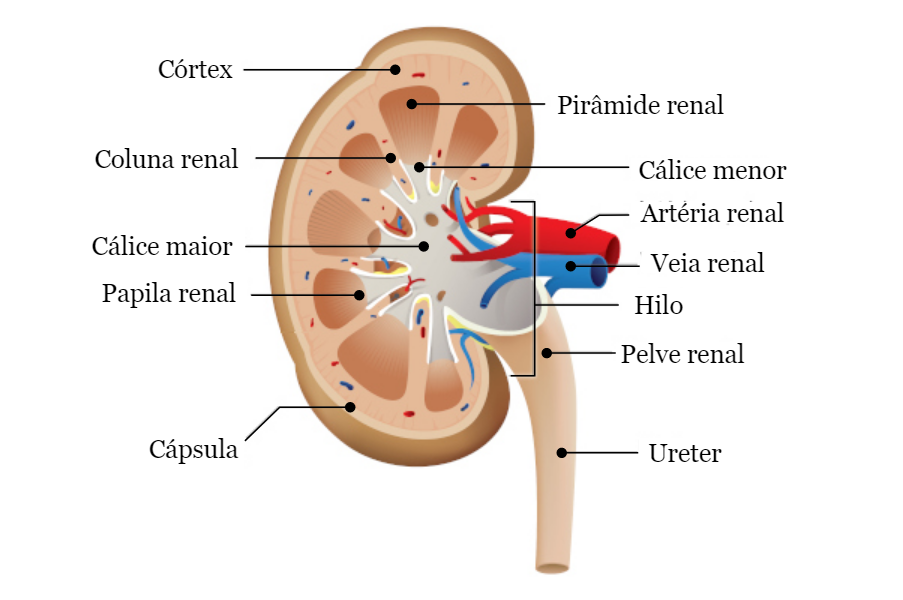
\includegraphics[width=0.85\textwidth]{figuras/anatomia-rins-interno.png}
    \legend{Fonte: \cite{vanessa_sardinha}.}
    \label{fig:anatomia-rins-interno}
\end{figure}

O principal papel dos rins é manter a homeostase. Isso significa que os rins gerenciam os níveis de fluidos, o equilíbrio eletrolítico e outros fatores que mantêm o ambiente interno do corpo consistente e confortável. Além disso, desempenham um amplo espectro de funções, tais como: remover uma série de resíduos a serem eliminados pela urina, reabsorção de nutrientes do sangue, manter o pH estável e regular a osmolaridade e a pressão arterial \cite{american_cancer,tim_newman,world_cancer}.

%Os rins são circuncidados em camadas externas complexas de fáscia e gordura, organizados da seguinte forma (profundo para superficial): cápsula renal, que é cápsula fibrosa resistente intimamente colada à superfície do órgão; gordura perirrenal, trata-se de uma coleção de gordura extraperitoneal; fáscia renal, responsável por envolver os rins e as glândulas supra-renais; e a gordura pararrenal, localizada principalmente na face póstero-lateral do rim~\cite{oliver_jones}. A Figura~\ref{fig:anatomia-rins-externo} ilustra as camadas externas do rim.

% \begin{figure}[!ht]
%     \centering
%     \caption{As camadas externas do rim.}
%     \includegraphics[width=0.8\textwidth]{figuras/anatomia-rins-externo2.png}
%     \legend{Fonte: Adaptado de \cite{oliver_jones}.}
%     \label{fig:anatomia-rins-externo}
% \end{figure}

Uma série de doenças pode afetar os rins, tais como: nefropatia diabética, insuficiência renal, hidronefrose renal, síndrome nefrótica, pedras nos rins e nefrite intersticial. Além disso, quando as células renais começam a se multiplicar de forma acelerada, podem surgir tumores renais. Os tumores renais podem ser benignos ou malignos. Os benignos não se espalham nem atacam os tecidos, mas os malignos podem ser agressivos a ponto de atingir outros órgãos por meio da corrente sanguínea. O câncer renal maligno mais comum é o carcinoma de células renais~\cite{SHUCH201585,tim_newman}.

A maioria dos casos de câncer renal tem cura com um diagnóstico precoce. Para iniciar o tratamento adequado do câncer renal, a segmentação acurada dos rins é necessária. Portanto, as informações estruturais do rim são analisadas por meio de exames de ultrassom, Ressonância Magnética (RM) ou TC de abdômen. Embora as imagens RM tenham sido usadas para segmentação renal em alguns estudos na literatura~\cite{goceri2011automatic,7424483}, a TC, dentre as modalidades disponíveis, é considerada o padrão ouro, especialmente para o diagnóstico de câncer precoce~\cite{kaur2016survey}. Além disso, a TC é muito útil no estadiamento (verificação da extensão para outros órgãos) e no planejamento terapêutico.

\section{Tomografia Computadorizada}
\label{sec:tumografia-computadorizada}

Para planejar o tratamento radioterápico, é necessário obter informações sobre os tumores renais, como tamanho e a localização exata. Para isso, é necessária uma imagem tridimensional detalhada da região do abdômen do paciente, geralmente realizada por meio do exame de TC. Essas informações são eventualmente usadas para orientar o radioterapeuta a produzir o melhor tratamento radioterápico para cada paciente.

A TC é um exame não invasivo, indolor e rápido, que combina uma série de imagens de raios-X obtidas de diferentes ângulos do corpo do paciente, produzindo sinais que são processados pelo computador para gerar imagens transversais (fatias) dos ossos, vasos sanguíneos e tecidos moles~\cite{Buzug2011}. Portanto, a TC funciona como outros exames de raios-X, mas fornece imagens mais detalhadas devido à emissão de vários feixes de raios-X ao mesmo tempo~\cite{gwynne2012image}.

Os feixes de raios-X são emitidos por uma fonte e coletados por um conjunto de detectores que permitem avaliar a quantidade de radiação que é absorvida pelos diferentes tecidos. Os detectores são posicionados no lado diametralmente oposto para captar os feixes que passam pelos objetos observados. Finalmente, os dados coletados pelos detectores são processados e digitalizados em \textit{pixels} que apresentam uma escala de cinza relacionada à atenuação sofrida pelos raios-X (medida da facilidade com que um material pode ser penetrado por um feixe de energia), expressa por uma escala numérica expressa em unidades Hounsfield (\textit{Hounsfield Units} - HU)~\cite{Buzug2011}. A HU é calculada com base em uma transformação linear do coeficiente de atenuação linear da linha de base do feixe de raios X~\cite{ADAMS2012277}.

Para a realização do exame, o paciente é posicionado no tomógrafo e imobilizado com suportes e fitas de fixação. O tomógrafo é uma máquina com um túnel no centro onde, durante o exame, o paciente fica deitado sobre uma mesa estreita que desliza dentro do túnel. Cortes axiais são feitos para verificar o posicionamento e alinhamento do paciente tomando como referência o isocentro (ponto onde os feixes de radiação se cruzam). Em seguida, são realizadas radiografias digitais (topograma), que programam as sequências de imagens (fatias) e a espessura dos cortes~\cite{Buzug2011,gwynne2012image}. A Figura~\ref{fig:equipamentoCT} ilustra um exemplo de equipamento de TC.

\begin{figure}[!ht]
    \centering
    \caption{Equipamento de TC.}
    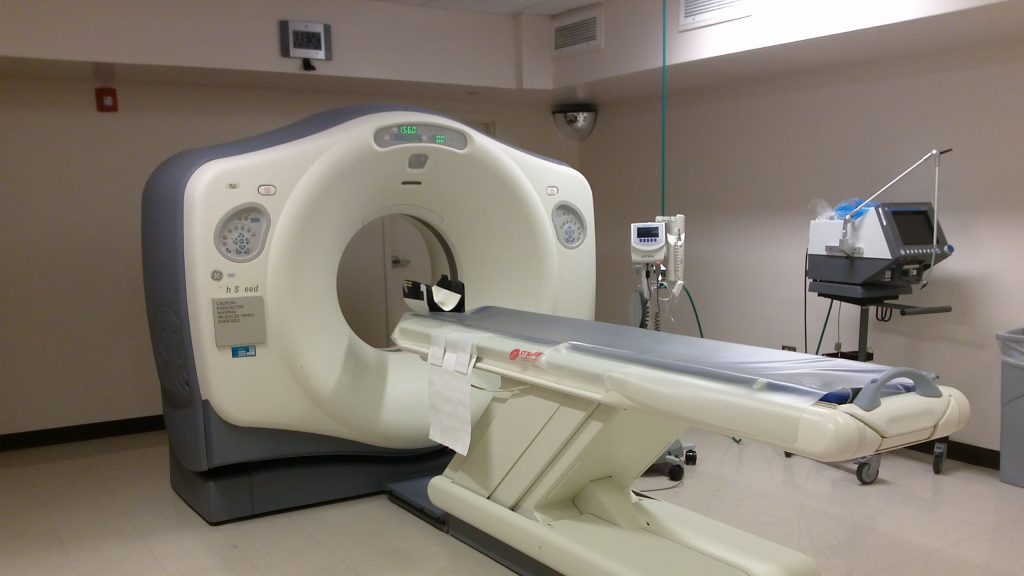
\includegraphics[width=0.9\textwidth]{figuras/equipamento-CT.jpg}
    \legend{Fonte: \cite{equipamento_CT}.}
    \label{fig:equipamentoCT}
\end{figure}

Uma vez que várias fatias sucessivas são coletadas pelo computador da máquina, elas são “empilhadas” digitalmente para formar uma imagem tridimensional do paciente que permite a identificação e localização mais fácil das estruturas básicas do corpo, bem como possíveis tumores ou anormalidades. Para melhorar a interpretação dos resultados e garantir diagnósticos mais precisos, a administração de contraste intravenoso pode ser solicitada antes da aquisição das imagens. Estas substâncias são usadas para aumentar a visibilidade e a diferenciação entre tumores e estruturas circundantes normais. O produto para se obter esse contraste é geralmente administrado por via oral (engolido) ou por via intravenosa (injetado). Após a obtenção das imagens, o contraste é eliminado pela urina.

\section{Processamento Digital de Imagens}
\label{sec:processamento-digital-imagens}

O processamento digital de imagens é definido como um conjunto de técnicas computacionais que transformam uma imagem de entrada em uma saída desejada~\cite{gonzalez2008digital}. Esse conjunto de técnicas permite extrair e identificar informações de imagens e melhorar a qualidade visual de aspectos estruturais, facilitando a percepção humana e a interpretação automática por meio de máquinas~\cite{pedrini2008analise}.

Existem vários algoritmos com propósitos muito específicos, que juntos formam a metodologia final. Portanto, uma metodologia difere de outra na forma como compõe suas etapas ou ferramentas, mas normalmente segue as etapas apresentadas por \citeonline{gonzalez2008digital}:

\begin{enumerate}
    \item Aquisição das imagens: as imagens são capturadas por meio de um dispositivo ou sensor e transformadas em um formato que pode ser processado posteriormente. Porém, como resultado desse processo, a imagem resultante pode apresentar falhas devido às condições de iluminação ou às características do dispositivo, por exemplo;
    
    \item Pré-processamento: o objetivo é melhorar a qualidade da imagem por meio de técnicas para reduzir o ruído, realçar o contraste e suavizar certas estruturas da imagem;
    
    \item Segmentação: consiste em localizar e extrair áreas de interesse contidas na imagem, com o objetivo de dividir a imagem isolando os diferentes objetos que a compõem;
    
    \item Representação e descrição: denominada de extração de características, pois extrai informações que podem ser usadas para discriminar classes de objetos;
    
    \item Reconhecimento e interpretação: reconhecimento é o processo que atribui um identificador aos objetos da imagem. A interpretação consiste em atribuir um significado ao conjunto de objetos reconhecidos.
\end{enumerate}

A saída de uma etapa é usada como entrada para a próxima etapa, sendo que cada entrada e saída pode ser ou não uma imagem digital. Uma metodologia de processamento de imagem pode conter apenas um subconjunto de todas as etapas apresentadas~\cite{BRAZ:2014}.

\section{Especificação do Histograma}
\label{sec:especificacao-histograma}

O histograma básico de uma imagem digital é uma função que gera a distribuição dos valores de intensidade presentes em uma imagem, com níveis de intensidade variando no intervalo de $\left[0, L - 1 \right]$. Ele é dado  pela  expressão  $h(r_{k}) = n_{k}$, onde $r_{k}$ é o  $k$-ésimo  nível de intensidade e $n_{k}$ é a quantidade de \textit{pixels} da imagem com intensidade $r_{k}$ \cite{gonzalez2008digital}. Portanto, o histograma é representado por um gráfico indicando o número de \textit{pixels}, eixo vertical, para cada nível de intensidade, eixo horizontal~\cite{pedrini2008analise}.

A especificação do histograma (\textit{histogram matching}) é o processo de transformar o histograma de uma imagem origem para corresponder ao histograma de uma imagem de referência, de modo que ambas tenham uma distribuição de \textit{pixels} semelhante~\cite{gonzalez2008digital}. Para especificar o histograma de uma determinada imagem, $h_{i}(x)$, com o histograma de uma imagem de referência, $h_{o}(y)$, primeiro é necessário equalizar os níveis da imagem original $h_{i}(x)$ para obter um histograma intermediário $h^{*}(z)$. A expressão usada para calcular esse mapeamento é definida na Equação~\ref{equacao:equalizar-histograma},

\begin{equation}
\label{equacao:equalizar-histograma}
y(i) = \frac{L - 1}{N}\sum_{i=0}^{L - 1}n_{i},
\end{equation}
onde $n_{i}$ representa o número de \textit{pixels} com nível $i$, e $N$ o total de \textit{pixels} da imagem com $L$ níveis de cinza.

A transformação $z = f(x)$ equaliza o histograma original $h_{i}(x)$ para o histograma intermediário $h^{*}(z)$, e $z = g(y)$ equaliza o histograma $h_{o}(y)$. Então, o mapeamento global dos níveis de intensidade necessários para produzir $h_{o}(y)$ a partir de $h_{i}(x)$ é obtido usando a transformação inversa $y = g^{-1}\left\{ f(x) \right\}$. Isso representa o mapeamento dos valores da imagem de entrada equalizada para seus valores mais próximos no histograma especificado. %A Figura~\ref{sec:especificacao-histograma} ilustra o procedimento de especificação do histograma.

% \begin{figure}[!ht]
%     \centering
%     \caption{Especificação do histograma.}
%     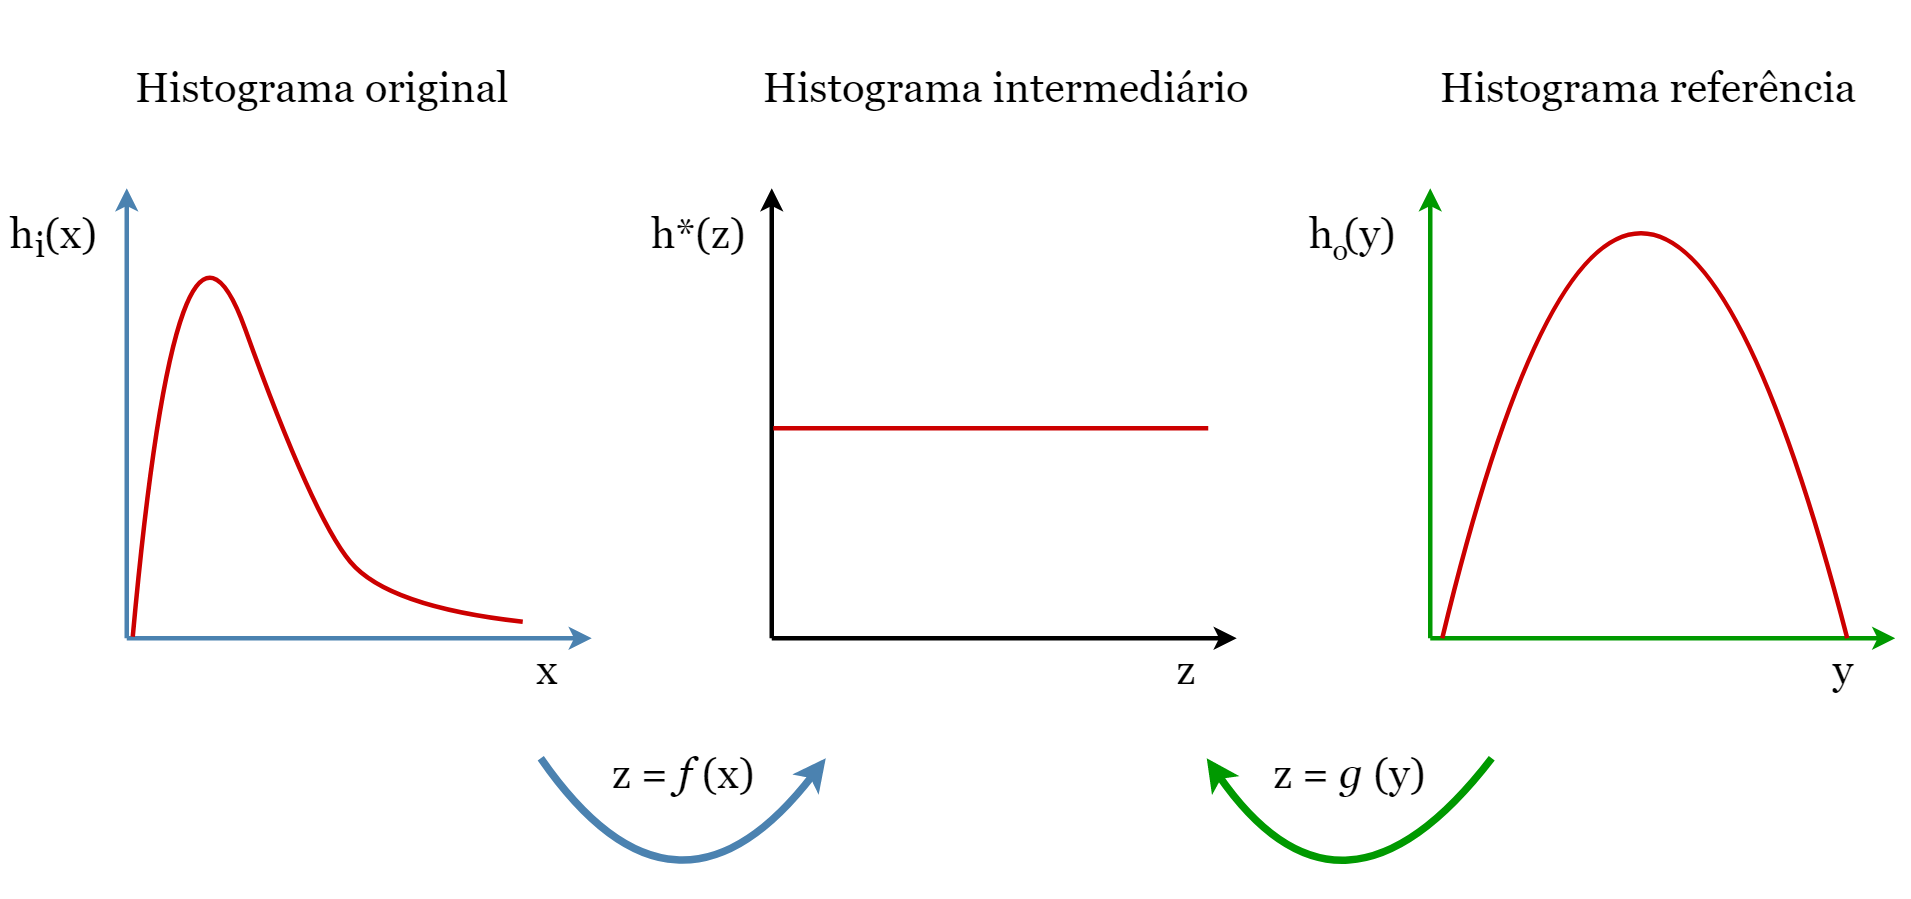
\includegraphics[width=0.9\textwidth]{figuras/especificacao-histograma.png}
%     \legend{Fonte: Adaptado de \cite{Giovanni2021}.}
%     \label{fig:especificacao_histograma}
% \end{figure}

Neste trabalho, a técnica de especificação do histograma foi usada na etapa de pré-processamento para mapear as intensidades inter-exames de TC baseado em um exame de referência de TC.

\section{Redes Neurais Artificiais}
\label{sec:redes-neurais-artificiais}

As Redes Neurais Artificiais (RNAs) são um ramo da Inteligência Artificial (IA), fundada na década de 1940, quando McCulloch e Pitts desenvolveram o primeiro modelo neural \cite{mcculloch1943logical}. O problema básico resolvido pelas RNAs é a aquisição indutiva de conceitos a partir de exemplos, a capacidade de aprender e generalizar a partir de dados, ou seja, imitar a capacidade humana de aprender com a experiência, torna as RNAs úteis na automatização do processo de aprendizado de regras de várias aplicações~\cite{MUKHOPADHYAY2011329}. 

%Em resumo, as RNAs são modelos matemáticos que usam uma coleção de unidades computacionais simples, chamadas de neurônios artificiais, interconectadas por uma grande quantidade de interconexões, denominadas sinapses artificiais~\cite{MUKHOPADHYAY2011329}. Esses modelos são comumente usados na tarefa de reconhecimento de padrões, como detecção de objetos, identificação de nódulos de câncer, reconhecimento de voz e reconhecimento facial~\cite{alanis2019artificial,baroni2020linguistic}.

Em resumo, as RNAs são esquemas computacionais que representam parcialmente as redes neurais biológicas existentes nos cérebros humanos ou animais, expressas por nós conectados (neurônios artificiais) organizados adequadamente em camadas. Todos os neurônios artificiais são conectados e capazes de transmitir sinais, geralmente números reais, por meio de suas conexões (sinapses artificiais)~\cite{MUKHOPADHYAY2011329,BERSIMIS201931}. Esses modelos são comumente usados na tarefa de reconhecimento de padrões, como detecção de objetos, identificação de nódulos de câncer, reconhecimento de voz e reconhecimento facial~\cite{alanis2019artificial,baroni2020linguistic}.

\subsection{Neurônio artificial}
\label{sec:neuronio-artificial}

O neurônio artificial é a unidade básica de uma RNA, fundamental para a construção de modelos mais poderosos. Em termos matemáticos, o neurônio artificial fornece uma saída para um determinado conjunto de entradas, conforme expresso na Equação~\ref{eq:neuronio-artificial},

\begin{equation}
\label{eq:neuronio-artificial}
f(x) = \sigma \left(\sum^n_{i=1}x_iw_i + b \right),
\end{equation}
em que $x_i$ é a entrada $i$, $w_i$ é o peso sináptico associado a entrada $i$, $b$ é o termo \textit{bias} e $\sigma$ é a função de ativação. Portanto, cada neurônio combina suas entradas e, em seguida, passa por uma função de ativação, que pode ser um filtro linear ou não-linear.

Em relação aos filtros não lineares, a função sigmoide e a função tangente hiperbólica são citadas como exemplos. Além delas, existem outra funções não lineares propostas como as chamadas~\textit{Rectified Linear Units} (ReLU) e \textit{Leaky Rectified Linear Unit} (Leaky ReLU), cuja velocidade de convergência em relação às supracitadas é até 6 vezes mais rápida~\cite{krizhevsky2012imagenet, maas2013rectifier}. Essas funções são expressas nas Equações~\ref{eq:relu} e \ref{eq:leakyrelu}, respectivamente,

\begin{equation}
\label{eq:relu}
\sigma(x) = max(0,x),
\end{equation}
\begin{equation}
\label{eq:leakyrelu}
\sigma(x) = max(0.1,x).
\end{equation}

\subsection{Redes \textit{Multilayer Percepton}}
\label{sec:redes-multilayer-percepton}

Embora existam inúmeras arquiteturas RNA, a arquitetura \textit{Multilayer Perceptron} (MLP) é a mais frequentemente encontrada na literatura \cite{PHAM2019302}. As MLPs são algoritmos de aprendizado supervisionado compostos por múltiplas camadas de neurônios, todas completamente conectadas às suas subsequentes. Os neurônios, por sua vez, implementam as funções de ativação não-linear determinadas. De acordo com \citeonline{hornik1989multilayer}, essas redes são capazes de aproximar qualquer função mensurável para qualquer grau de precisão desejado.

De modo geral, uma MLP é composta por uma camada inicial, que recebe os dados de entrada do modelo, seguida por uma ou mais camadas intermediárias (ocultas/escondidas) e, por fim, uma camada de saída~\cite{hornik1989multilayer}. A Figura~\ref{fig:rna} ilustra uma arquitetura básica de MLP com apenas uma camada oculta.

\begin{figure}[!ht]
    \centering
    \caption{Rede \textit{Multilayer Percepton}.}
    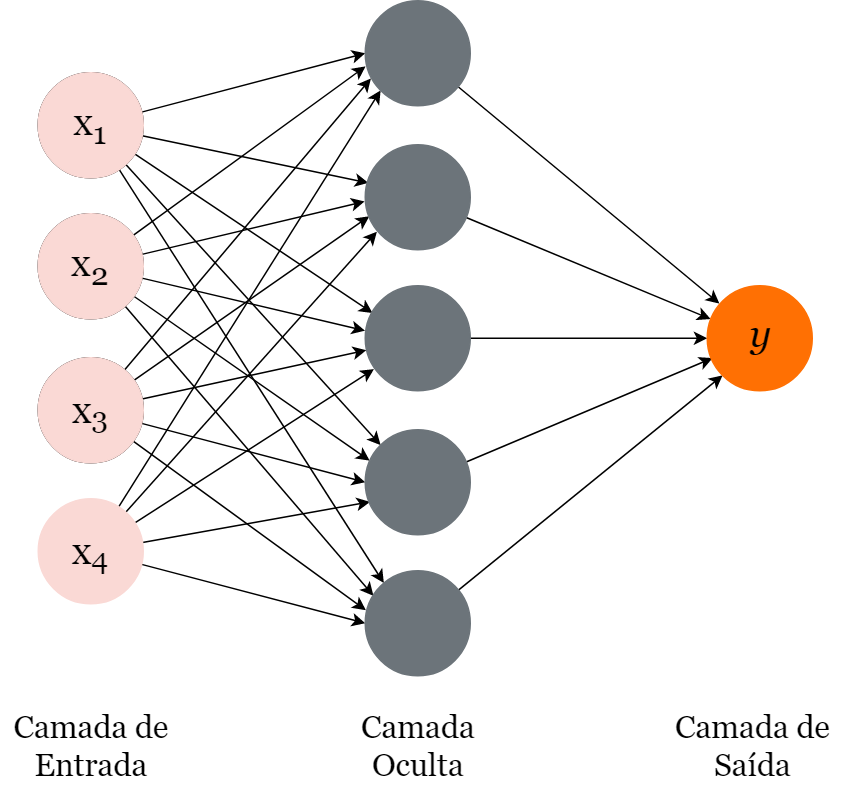
\includegraphics[width=0.45\textwidth]{figuras/RNA.png}
    \legend{Fonte: Elaborado pela autora.}
    \label{fig:rna}
\end{figure}

Os neurônios de cada camada são organizados e conectados uns aos outros em uma estrutura de múltiplas camadas \textit{feedforward}. Em outras palavras, cada camada é totalmente conectada com sua camada adjacente e produz um vetor de saída de acordo com o vetor da camada anterior~\cite{BERSIMIS201931}. A saída de cada camada é calculada aplicando a função de ativação de cada neurônio a todos os neurônios da camada. A Equação~\ref{eq:mlp} descreve a saída de uma camada,

\begin{equation}
\label{eq:mlp}
y^l = \sigma(W^ly^{l-1} + b^l),
\end{equation}
em que $y^l$ é o vetor de saída, $W^l$ é a matriz dos pesos aplicados a cada par de neurônio da camada $l$ e $l-1$, e $b^l$ é o vetor do termo \textit{bias} de cada neurônio da camada $l$. Para treinar efetivamente as MLPs, o algoritmo de \textit{backpropagation} é aplicado.

\subsection{\textit{Backpropagation}}
\label{sec:backpropagation}

Durante o treinamento de uma MLP, uma função de erro é definida para calcular o erro das predições do modelo com base na saída esperada para os dados de entrada fornecidos. O objetivo do treinamento é minimizar o erro total da rede (soma das funções de erro aplicadas a todos os exemplos de uma base de imagens). Para isso, as MLPs usam um algoritmo denominado \textit{backpropagation}.

O algoritmo \textit{backpropagation} é caracterizado por dois passos consecutivos: primeiro, os dados são enviados para a camada de entrada da rede, e trafegam pela rede, camada por camada, sendo transformados por meio de cálculos realizados até que, na camada de saída, uma resposta seja produzida; segundo, a saída obtida é comparada com a saída desejada da entrada correspondente e um valor de erro é calculado. Em seguida, os erros derivados com relação aos parâmetros da rede são propagados novamente, da camada de saída até a camada de entrada, desta forma, os pesos das conexões nas camadas ocultas são modificados à medida que o erro é retropropagado. O processo continua várias vezes até que uma melhoria desejada na previsão do modelo seja alcançada.

Os passos do algoritmo~\textit{backpropagation} são brevemente apresentados a seguir. Os itens 1, 2 e 3 estão relacionados ao \textit{feedforward} e o \textit{backpropagation} inicia no item 4.

\begin{enumerate}
	\item Inicializar os valores dos pesos sinápticos de cada neurônio aleatoriamente;
	
	\item Apresentar as entradas da rede em um vetor ${x_1 , x_2 , ..., x_n}$ de características e especificar um vetor ${d_1 , d_2 , ..., d_n}$ de saídas desejadas;
	
	\item Calcular as saídas da rede ${y_1 , y_2 , ..., y_n}$ conforme a Equação~\ref{eq:neuronio-artificial};
	
	\item Reajustar os pesos começando pelos neurônio da camada de saída, retropropagando até a camada de entrada, de acordo com a Equação~\ref{eq:bp1},
    \begin{equation} \label{eq:bp1}
    	w_{ij} (t + 1)= w_{ij} (t) + \eta \delta_j x_i,
    \end{equation}
	onde $w_{ij}$ é o peso do neurônio $j$ em uma iteração $t$, $x_i$ corresponde a um neurônio de saída ou de entrada, $\eta$ é a taxa de aprendizagem e $\delta_j$ é um erro de gradiente para o neurônio $j$. Se $j$ for um neurônio de saída, então $\delta_j$ é definido pela Equação~\ref{eq:bp2},
	\begin{equation}
	\label{eq:bp2}
    	\delta_j = y_j (1 - y_j)(d_j - y_j),
    \end{equation}
	onde $d_j$ denota a saída desejada e $y_j$ é a saída desejada da rede. Se o neurônio $j$ for um neurônio oculto, então $\delta_j$ é definido pela Equação~\ref{eq:bp3},
	\begin{equation}
	\label{eq:bp3}
        \delta_j = x_j (1 - x_j) \sum_{k}\delta_k w_{jk},
    \end{equation}
	onde $k$ denota todos os neurônios da camada após a camada do neurônio $j$;
	\item Retornar ao passo 2 até que uma determinada condição seja satisfeita.
\end{enumerate}

É importante ressaltar que a taxa de aprendizado ($\eta$) influencia a magnitude das mudanças dos pesos, desempenhando papel fundamental no aprendizado do modelo. Taxas de aprendizados muito pequenas implicam em pequenas variações, o que torna o modelo lento e aumentam as chances de parar em mínimos locais. No entanto, altas taxas de aprendizado tendem a produzir grandes oscilações, o que compromete o processo de aprendizado do modelo. A taxa de aprendizado é introduzida na rede para permitir uma convergência mais rápida ao valor ótimo desejado e ao mesmo tempo evitar que a rede oscile, diminuindo a taxa de aprendizado quando o erro tende a aumentar~\cite{silva2004algoritmos,haykin2007redes,silva2010redes}.

%Uma vez que a rede está treinada e o erro está em um nível satisfatório, a rede pode ser usada como uma ferramenta para classificar novos dados.

\section{Aprendizado Profundo}
\label{sec:aprendizado-profundo}

Durante o processo de aprendizagem, humanos e animais são inicialmente conduzidos a interpretar e compreender conceitos mais simples, a fim de aprender conceitos mais complexos a partir de conceitos previamente observados ao longo de suas vidas~\cite{fernandes2013redes}. Esse processo de aprendizagem, denominado aprendizado profundo, sugere uma divisão em camadas hierárquicas do cérebro com diferentes responsabilidades~\cite{hubel1998early}.

O aprendizado profundo é uma subárea do aprendizado de máquina que usa arquiteturas hierárquicas para aprender abstrações de alto nível em um conjunto de imagens. É uma abordagem em evolução e tem sido amplamente usada em domínios tradicionais de inteligência artificial, como análise semântica, transferência de aprendizado, processamento de linguagem natural e visão computacional. Existem três fatores importantes para o crescimento do aprendizado profundo: o aumento da capacidade de processamento dos \textit{chips} gráficos, os avanços consideráveis nos algoritmos de aprendizado de máquina e o custo significativamente reduzido do \textit{hardware} de computação~\cite{GUO201627}.

As técnicas de aprendizagem profunda apresentam múltiplas camadas de processamento não linear para reconhecimento de padrões de forma semelhante ao cérebro~\cite{LeCun2015}. Diferente das RNAs tradicionais, essas técnicas permitem a extração automática de características do conjunto de treinamento, sem a necessidade de uma série de técnicas de processamento de imagens e reconhecimento de padrões~\cite{hua2015computer}. Como resultado, as etapas de extração, seleção e classificação de características são abstraídas no próprio modelo, com pouca intervenção humana~\cite{hua2015computer,cheng2016computer}.

Atualmente, existem inúmeras técnicas de aprendizagem profundas disponíveis na literatura, como as redes neurais convolucionais, redes neurais recorrentes, redes de crença profunda, redes de memória de longo prazo, os auto-codificadores esparsos empilhados, entre outras. As diferentes arquiteturas têm diferentes vantagens com base na aplicação e nas características dos dados envolvidos. Por exemplo, em visão computacional, as redes neurais convolucionais são preferidas e, em sequências e modelagem de séries temporais, as redes neurais recorrentes. O aprendizado profundo é um campo em rápida evolução e arquiteturas mais novas com algoritmos de aprendizado mais recentes são frequentemente desenvolvidas para suportar a necessidade de desenvolver máquinas eficientes semelhantes a humanos em diferentes áreas de aplicação~\cite{SENGUPTA2020}.

\subsection{Redes Neurais Convolucionais}
\label{sec:redes-neurais-convolucionais}

As redes neurais convolucionais (\textit{Convolutional Neural Networks} - CNN) são modelos biologicamente inspirados capazes de construir um aprendizado hierárquico de características~\cite{726791, 6932467}. Essa arquitetura é bastante popular em tarefas de visão computacional, como detecção, segmentação e classificação de imagens e vídeos de vários domínios.

Geralmente, a CNN usa em sua arquitetura três tipos de camadas: convolução, subamostragem e completamente conectada~\cite{726791}. As camadas de convolução extraem características de baixo nível importantes da imagem de entrada, como textura simples e bordas. À medida que mais camadas de convolução são adicionadas, características de alto nível são extraídas. As camadas de subamostragem reduzem a resolução dos mapas de características, mantendo as informações de características. Finalmente, a camada totalmente conectada conecta a rede à camada discriminante (camada de saída), que fornece a saída desejada~\cite{LeCun2015}. A Figura~\ref{fig:cnn} ilustra uma arquitetura básica de CNN, em seguida, os detalhes de cada camada são apresentados.

\begin{figure}[!ht]
    \centering
    \caption{Exemplo de uma arquitetura CNN.}
    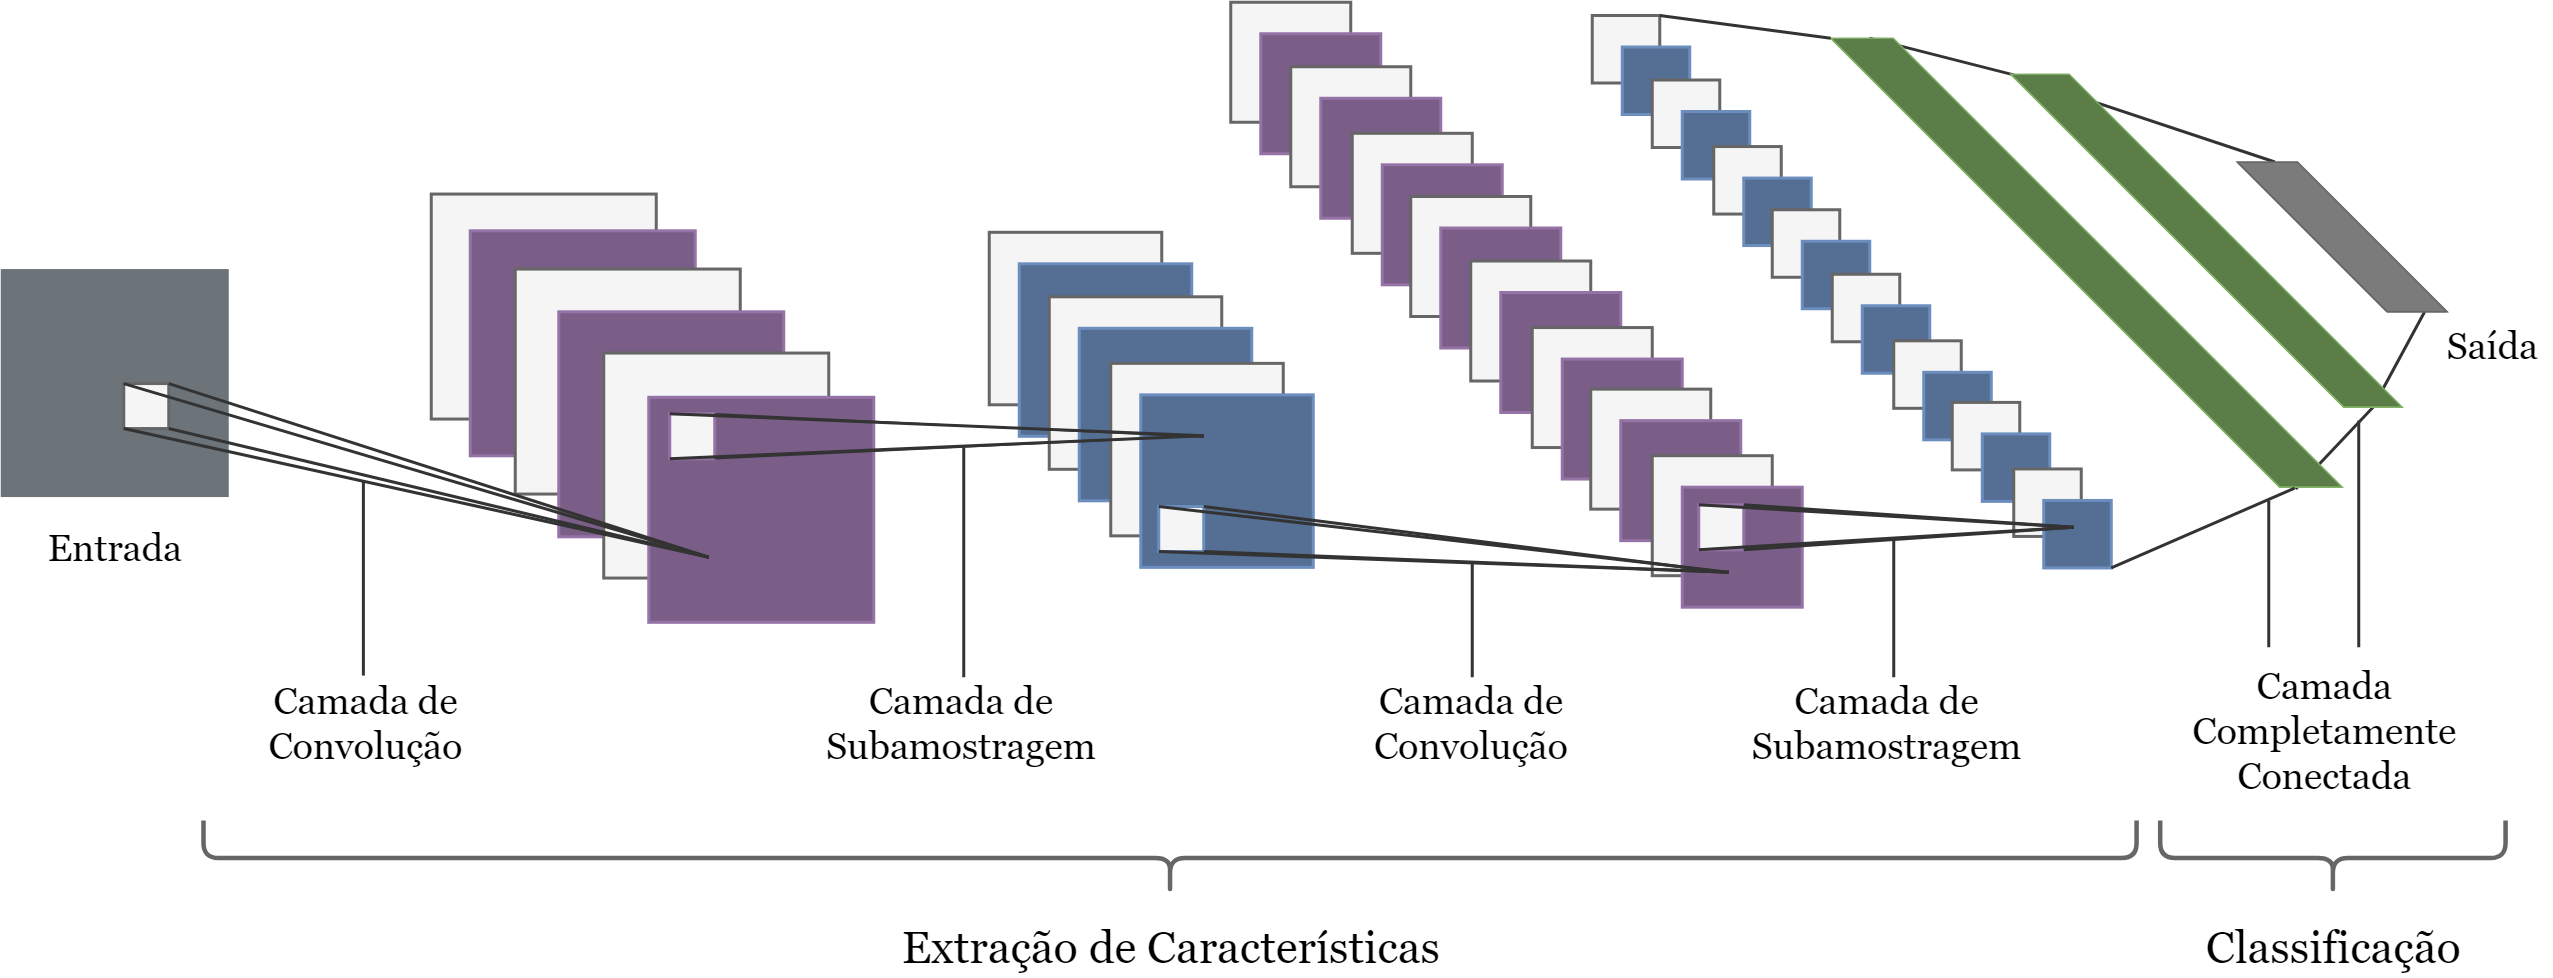
\includegraphics[width=1\textwidth]{figuras/arquitetura-CNN.png}
    \legend{Fonte: Adaptado de \cite{LIU201711}.}
    \label{fig:cnn}
\end{figure}

\subsubsection{Camada de Convolução}
\label{sec:camada-convolucao}

As camadas de convolução são compostas por filtros treináveis aplicados individualmente na imagem de entrada da rede, gerando diversos mapas de características. Os filtros são definidos por uma pequena área ($3\times3$, $5\times5$, $7\times7$ \textit{pixels}) e cada neurônio é ligado apenas aos neurônios nas proximidades da camada anterior. Portanto, para cada filtro aplicado a uma imagem de entrada, pode existir um neurônio conectado com a saída de um subconjunto de neurônios da camada anterior. Os pesos são compartilhados entre os neurônios, fazendo com que os filtros aprendam os padrões frequentes que ocorrem em qualquer parte da imagem~\cite{5537907,GUO201627}. O processo de convolução em uma imagem é ilustrado na Figura~\ref{fig:camada-convolucao}.

\begin{figure}[!ht]
    \centering
    \caption{Ilustração de uma operação de convolução.}
    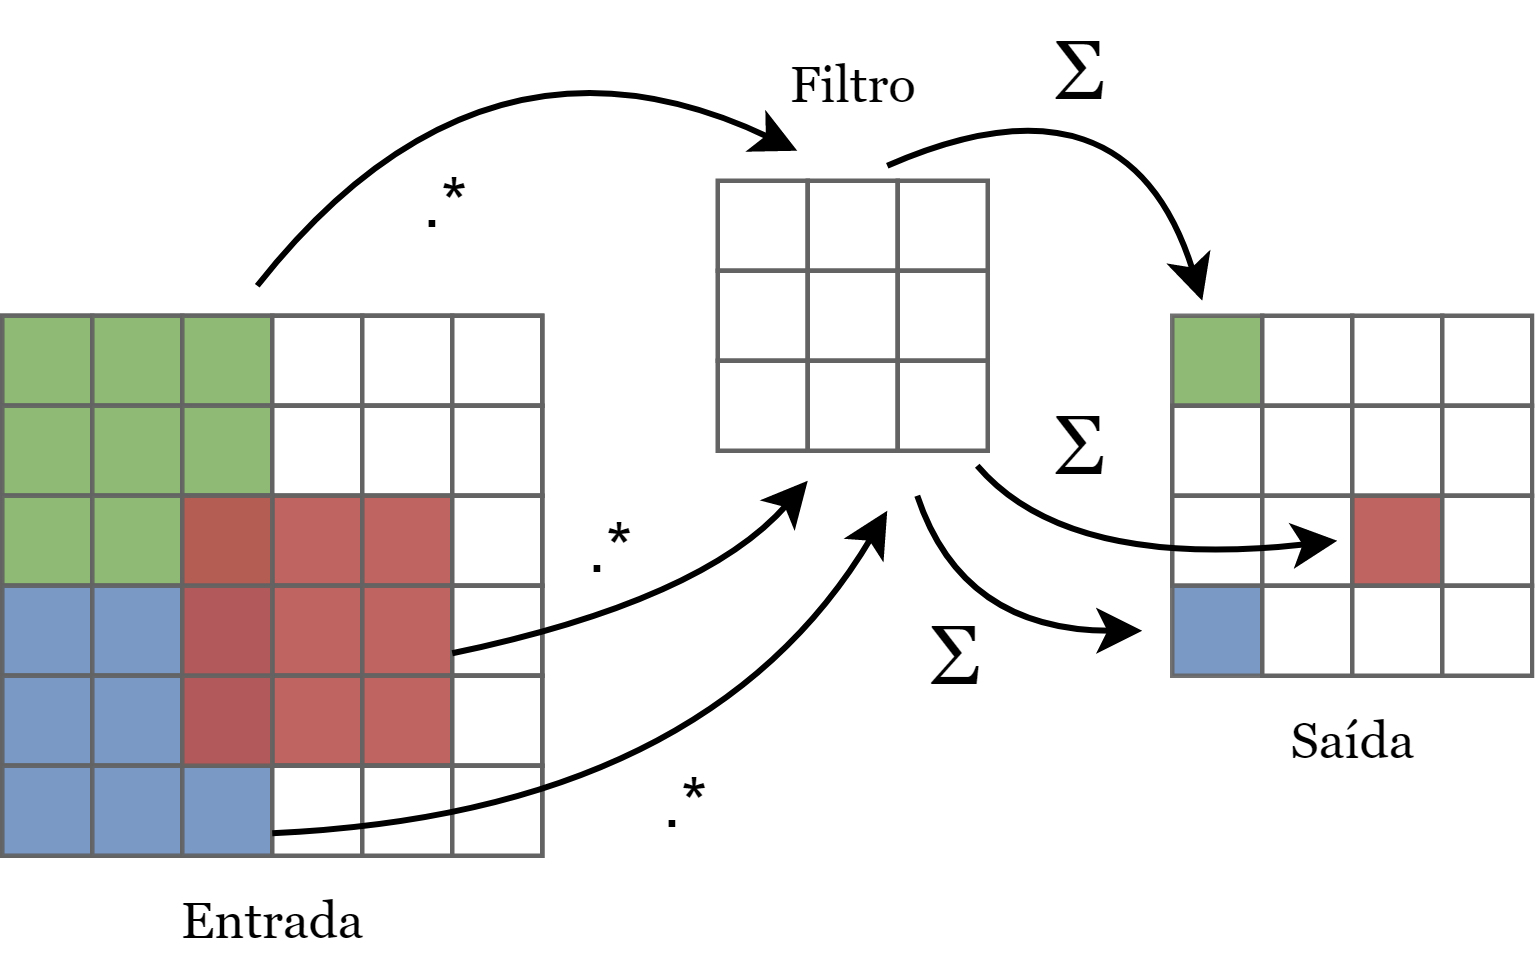
\includegraphics[width=0.57\textwidth]{figuras/camada-convolucao.png}
    \legend{Fonte: Adaptado de \cite{hafemann:14}.}
    \label{fig:camada-convolucao}
\end{figure}

Após gerar mapas de características, uma camada de ativação não linear é aplicada~\cite{WU2020}. Ao fim do treinamento da rede, cada filtro será responsável por detectar uma característica específica da imagem, ou de parte dela~\cite{hafemann:14}.

\subsubsection{Camada de Subamostragem}
\label{sec:camada-subamostragem}

As camadas de subamostragem são geralmente subsequentes às camadas de convolução e são usadas para reduzir as resoluções dos mapas de características produzidos pelas camadas de convoluções anteriores e selecionar as características invariantes a deslocamentos e distorções~\cite{5537907,hafemann:14}.

A subamostragem consiste em aplicar filtros nos mapas de características e usar operações como média (\textit{average pooling}) ou valor máximo (\textit{max-pooling}) para extrair valores dessas sub-regiões. A Figura~\ref{fig:camada-subamostragem} ilustra a subamostragem com a aplicação da operação \textit{max-pooling} deslizando uma janela de tamanho 3 com passo igual a 1, na qual apenas o valor máximo de \textit{pixel} da janela de convolução é mantido. Ou seja, em uma máscara $3\times3$ com 9 valores, apenas o maior valor de \textit{pixel} entre eles permanecerá.

\begin{figure}[!ht]
    \centering
    \caption{Ilustração da camada de subamostragem.}
    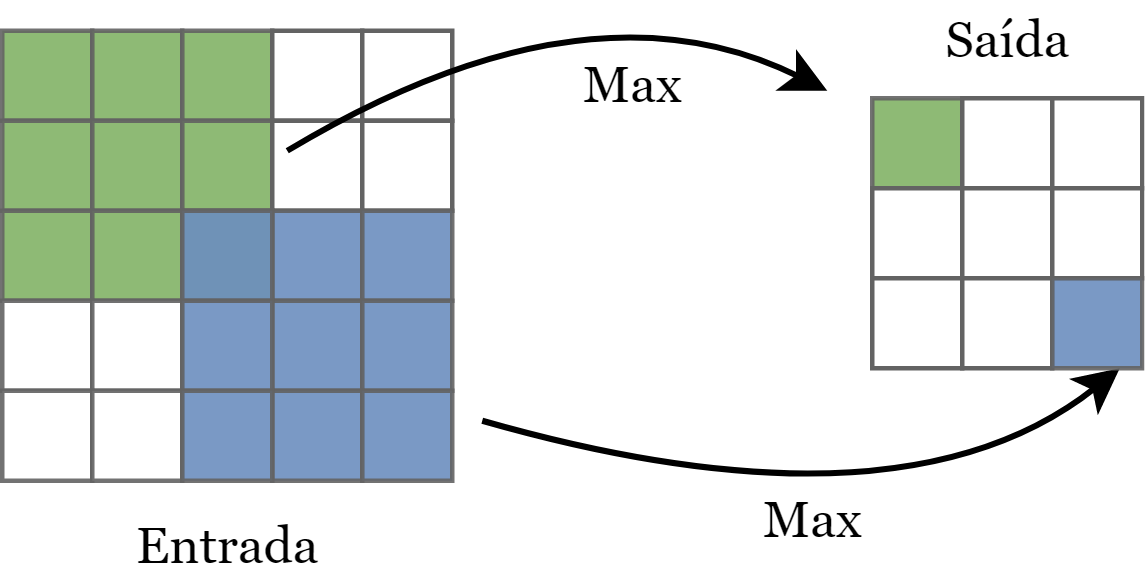
\includegraphics[width=0.55\textwidth]{figuras/camada-subamostragem2.png}
    \legend{Fonte: Adaptado de \cite{hafemann:14}.}
    \label{fig:camada-subamostragem}
\end{figure}

Existem também as operações de \textit{upsampling}. Basicamente, elas se comportam como o inverso das camadas de~\textit{max-pooling}, ou seja, dobram a resolução dos mapas de características da camada anterior por operações de interpolação~\cite{long2015fully}. No entanto, é configurável.

\subsubsection{Camada Completamente Conectada}
\label{sec:camada-completamente-conectada}

Depois de extrair as características com as camadas de convolução e subamostragem, os mapas de características podem ser usados como entrada para as camadas totalmente conectadas, que por sua vez são responsáveis por classificar os padrões de entrada. Os neurônios em uma camada totalmente conectada têm conexões com todas as ativações na camada anterior, semelhante à estrutura do MLP (Seção~\ref{sec:redes-multilayer-percepton}).

Uma vez que a rede esteja treinada em um nível satisfatório, a rede pode ser usada como uma ferramenta para classificar novos dados. Neste trabalho, arquiteturas baseadas nos conceitos de redes neurais convolucionais são usadas para segmentar rins e tumores renais em imagens tomográficas.

\section{Arquitetura U-Net}
\label{sec:arquitetura-unet}

Para realizar a segmentação dos rins e reconstrução dos tumores renais em imagens de TC, foi usada como base a arquitetura da U-Net~\cite{He7780459}, que é uma rede capaz de generalizar mesmo em domínio de baixa variância.

A U-Net é uma RNA completamente convolucional proposta para segmentação de imagens biomédicas \cite{ronneberger2015u}, que desde 2015 vem superando os métodos existentes em diversos desafios biomédicos de segmentação de imagens. Essa rede é um tipo específico de rede profunda e avançada cuja arquitetura consiste em um caminho de contração e um caminho de expansão simétrico. A principal estratégia que diferencia a U-Net das outras arquiteturas totalmente convolucionais (\textit{Fully Convolutional Network} - FCN) é a combinação entre os mapas de características no estágio de contração e seus correspondentes simétricos no estágio de expansão, o que permite a propagação de informações de contexto para os mapas de características de alta resolução. A Figura~\ref{fig:arquitetura_unet} ilustra a arquitetura e as camadas que constituem a U-Net.

\begin{figure}[!ht]
    \centering
    \caption{Arquitetura U-Net.}
    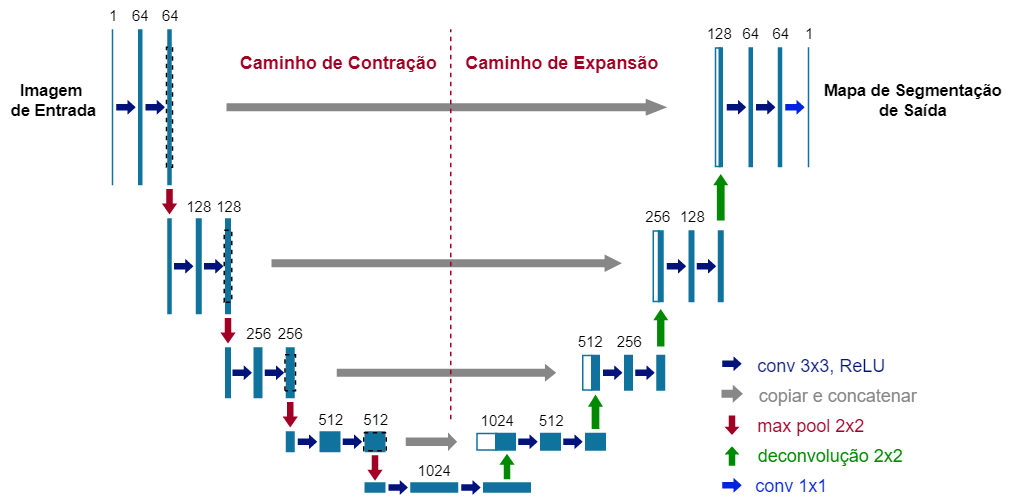
\includegraphics[width=1\textwidth]{figuras/arquitetura-Unet.png}
    \legend{Fonte: Adaptado de \cite{ronneberger2015u}.}
    \label{fig:arquitetura_unet}
\end{figure}

O caminho de contração (lado esquerdo) captura o contexto e o caminho de expansão (lado direito) simétrico permite uma localização precisa. O caminho de contração é uma arquitetura CNN tradicional, várias aplicações repetidas de duas convoluções $3\times3$, cada uma acompanhada por uma função de ativação ReLU e uma operação de subamostragem com operação de \textit{max-pooling} $2\times2$, reduzindo a largura e a altura da imagem, com passo (\textit{stride}) 2 para subamostragem. Em cada etapa de subamostragem, o número de canais de características dobra.  No caminho de contração as camadas de 1 a 5 são compostas por convoluções de 64, 128, 256, 512 e 1024 filtros, respectivamente.

O caminho de expansão consiste em um levantamento do mapa de características seguido de uma deconvolução (\textit{upsampling}) $2\times2$ que faz a metade do número de canais de características. Posteriormente, uma junção é feita com o mapa de características correspondentemente cortado do caminho de contratação e duas convoluções 3x3, cada uma seguida por uma função de ativação ReLU. Essa etapa do caminho expansivo é importante devido à perda de \textit{pixels} de borda em cada convolução no caminho de contratação. Na última camada é usada uma convolução 1x1 para mapear cada vetor de características para o número desejado de classes.

Em resumo, a U-Net pode ser treinada do início ao fim com poucas imagens, onde a U-Net simplesmente concatena os mapas de características do codificador para mapear mapas de características do decodificador em todas as etapas para formar uma estrutura como escada. As conexões de concatenação nesta arquitetura permitem que o decodificador aprenda as características relevantes que são perdidas quando o codificador é agrupado em cada fase.

\section{Arquitetura DeepLabv3+}
\label{sec:deeplabv3+}

Para obter a segmentação de tumores renais em TC, foi usada como base a arquitetura de última geração DeepLabv3+~\cite{chen2018encoder}, que é um modelo forte para codificar informações contextuais e refinar os resultados da segmentação, especialmente ao longo dos limites do objeto.

Como descrito anteriormente, as redes neurais profundas usam estruturas de codificador-decodificador para tarefas de segmentação semântica. O codificador extrai informações contextuais em várias escalas, enquanto o decodificador captura os limites dos objetos de forma mais clara, recuperando gradualmente as informações espaciais para reconstruir a saída~\cite{chen2018encoder}. Na arquitetura DeepLabv3+ o codificador padrão usado é o Xception (\textit{Extreme Inception})~\cite{chollet2017xception}. Em resumo, o Xception é uma extensão da arquitetura Inception que substitui os módulos Inception padrão por convoluções separáveis em profundidade (\textit{depth wise separable convolution}).

A Figura~\ref{fig:arquitetura_DeepLabv3+} ilustra a arquitetura DeepLabv3+. As imagens de entrada da rede passam por uma estrutura de codificador-decodificador. Na fase de codificação, as características extraídas do codificador Xception são usadas como entrada para as operações de \textit{Atrous Convolution} e \textit{Atrous Spatial Pyramid Pooling} (ASPP). O \textit{Atrous Convolution} captura características em escalas múltiplas (\textit{rate} = 6, \textit{rate} = 12 e \textit{rate} = 18), e o ASPP é uma operação de \textit{pooling} que ajuda a calcular objetos em escalas diferentes. Essas operações fazem a ponte entre a codificação e a decodificação~\cite{chen2018encoder}.

\begin{figure}[!ht]
    \centering
    \caption{Arquitetura DeepLabv3+.}
    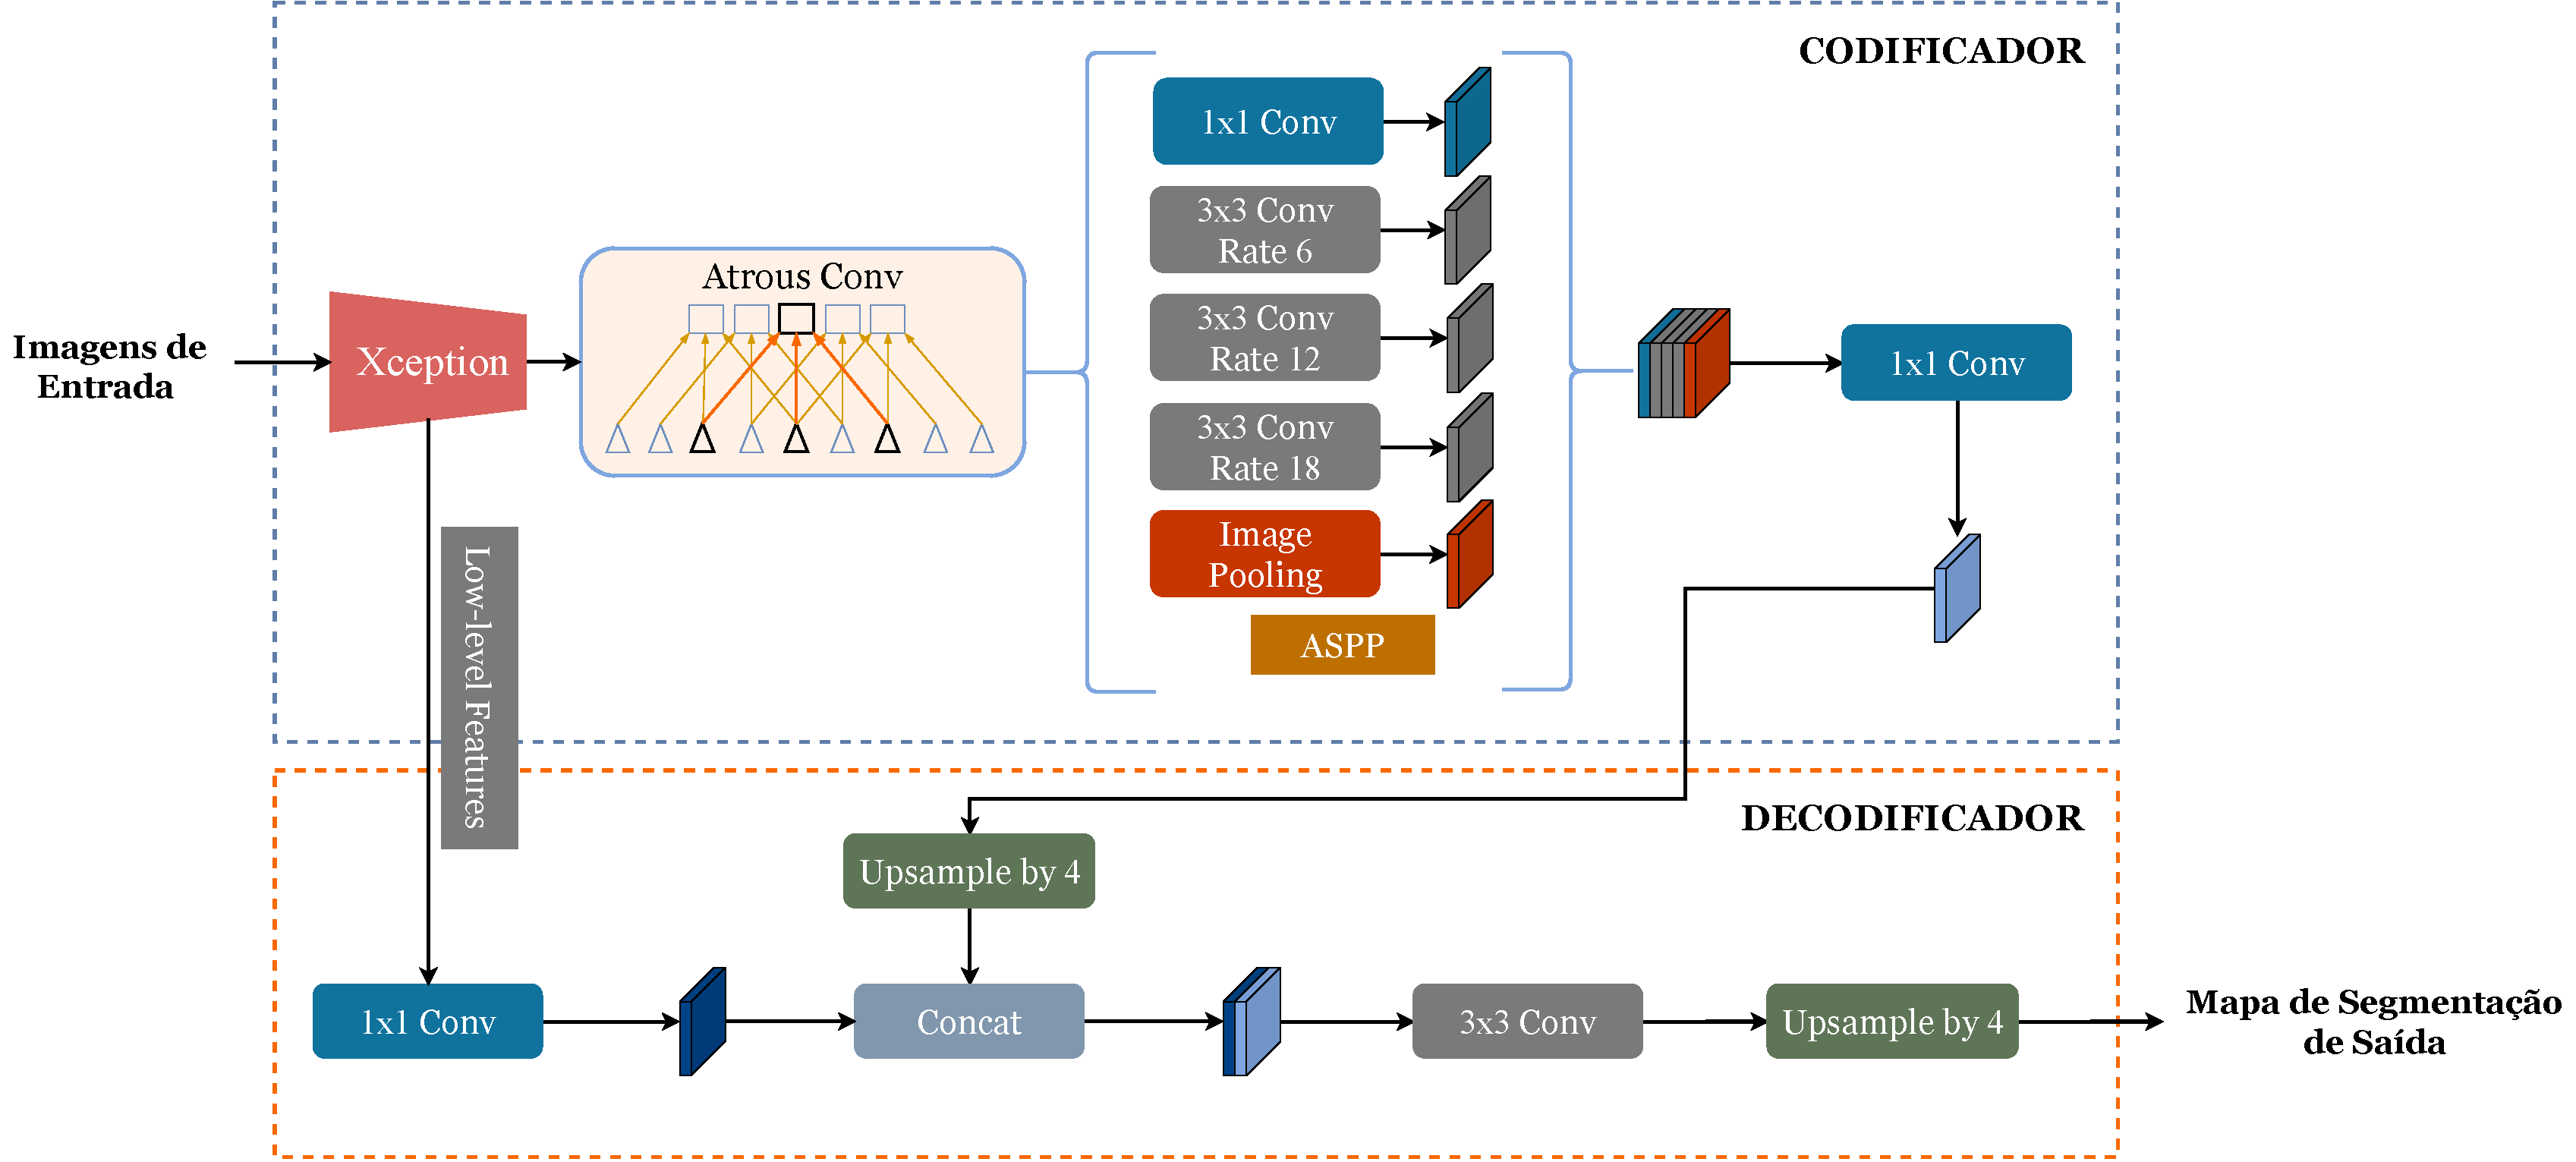
\includegraphics[width=1\textwidth]{figuras/arquitetura_DeepLabv3+.pdf}
    \legend{Fonte: Adaptado de~\cite{chen2018encoder}.}
    \label{fig:arquitetura_DeepLabv3+}
\end{figure}

Na fase de decodificação, as informações extraídas na codificação são usadas para reconstruir a saída. Assim, após as operações de \textit{Atrous Convolution} e ASPP, a operação de \textit{upsampling} é aplicada usando um filtro bilinear de fator 4. Posteriormente, concatena-se com os \textit{low-level features} (características de baixo nível) correspondentes da saída do codificador Xception, após passar por uma convolução 1 × 1 para reduzir o número de canais. Após a concatenação, algumas convoluções 3 × 3 são aplicadas para refinar as características, seguidas por outro \textit{upsampling} bilinear simples de fator 4. Além disso, é usada a \textit{depth wise separable convolution}, que é uma operação para reduzir o custo de computação e vários parâmetros, mantendo o desempenho~\cite{chen2018encoder}.

\section{\textit{Data Augmentation}}
\label{sec:data-augmentation}

\textit{Data augmentation} é uma técnica comumente usada na literatura para aumentar o tamanho e a diversidade dos conjuntos de treinamento. Em visão computacional, o \textit{data augmentation} se tornou uma técnica de regularização implícita comum para combater o \textit{overfitting} em modelos de aprendizado profundo e é usado para melhorar o desempenho do modelo~\cite{kukavcka2017regularization, mikolajczyk2018data}.

O aumento de dados é semelhante à imaginação ou sonho. Os seres humanos imaginam diferentes cenários com base na experiência. A imaginação ajuda a compreender melhor o mundo. Os métodos de \textit{data augmentation}, podem “imaginar” alterações nas imagens, para que tenham um melhor entendimento delas~\cite{shorten2019survey}. Portanto, técnicas são usadas para aumentar a diversidade da base de imagens aplicando transformações aleatórias, como transformações geométricas (rotação, translação, espelhamento, etc.) e filtros para realçar imagens (CLAHE, filtros de contraste, etc.), por exemplo.

No entanto, existem algumas desvantagens de usar o \textit{data augmentation}, como memória e tempo de treinamento adicionais, e alto custo computacional~\cite{shorten2019survey}. Estas desvantagens ocorrem quando o \textit{data augmentation} é gerado \textit{offline} (em disco) e adicionado ao conjunto de treinamento. Como não é prático nem eficiente armazenar os dados aumentados na memória, técnicas de \textit{data augmentation} em tempo real são usadas como uma solução para minimizar essas desvantagens. Como o nome sugere, o aumento é aplicado em tempo real, as transformações são realizadas em mini-lotes e, em seguida, inseridas ao treinamento do modelo. Dessa forma, as variações criadas artificialmente a partir de imagens existentes não precisam ser salvas na memória do disco, o que reduz o tempo de acesso ao disco para realizar operações de leitura e escrita.

No método proposto, o \textit{data augmentation} foi realizado em tempo real (\textit{online})~\cite{shorten2019survey}, não sendo necessário incluir novas imagens de \textit{data augmentation} no conjunto de treinamento original, uma vez que foi aplicado diretamente ao conjunto de treinamento. Desta forma, novas imagens são geradas atualizando constantemente o próprio conjunto de treinamento. Essa técnica proporcionou maior poder de generalização e desempenho do modelo e baixo consumo de recursos de máquina. Na subseção~\ref{sec:resultados-candidatores-tumores-renais-regiao-renal} são apresentadas as operações de \textit{data augmentation} em tempo real que foram aplicadas neste estudo.

\section{Métricas de Desempenho}
\label{sec:metricas-de-desempenho}

Para validar os resultados obtidos por um método proposto, quantificações de resultados são comumente adotadas. Esta atividade tem como objetivo avaliar o desempenho do método desenvolvido por meio da análise estatística dos resultados. Neste trabalho, as métricas usadas são comumente aplicadas em sistemas CAD/CADx para análise de imagens médicas: acurácia, sensibilidade, especificidade, coeficiente de similaridade Dice e índice de Jaccard~\cite{taha2015metrics, bland2015introduction}.

%Para o cálculo das métricas, baseou-se na matriz de confusão (Figura~\ref{fig:matriz_confusao}), que leva em consideração 4 variáveis: (1) Verdadeiro Positivo (VP) indica os casos realmente positivos detectados; (2) Falso Positivo (FP) denota os casos negativos erroneamente detectados como positivos; (3) Verdadeiro Negativo (VN) denota os casos negativos verdadeiramente detectados; e (4) Falso Negativo (FN) denota os casos positivos detectados erroneamente como negativos.

O cálculo das métricas é baseado na matriz de confusão (Figura~\ref{fig:matriz_confusao}), que leva em consideração quatro variáveis: Verdadeiro Positivo (VP) indica a classificação correta dos \textit{pixels} da classe positiva, ou seja, o alvo de segmentação (rins ou tumores renais, dependendo do modelo); Falso Positivo (FP) denota a classificação errônea dos \textit{pixels} da classe negativa como classe positiva; Verdadeiro Negativo (VN) indica a classificação correta dos \textit{pixels} da classe negativa; e Falso Negativo (FN) trata-se da classificação errônea dos \textit{pixels} da classe positiva como classe negativa.

\begin{figure}[!ht]
    \centering
    \caption{Matriz de confusão.}
    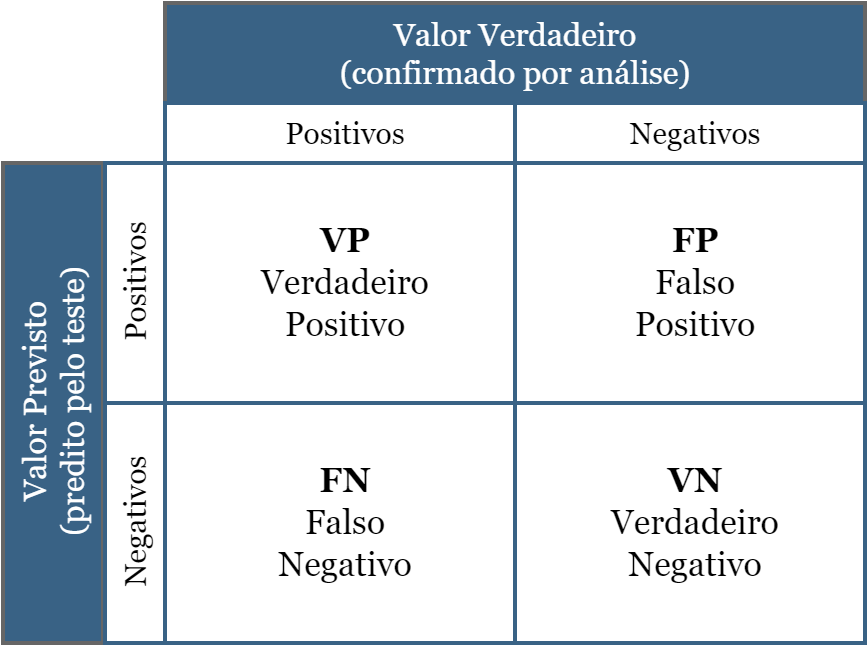
\includegraphics[width=0.4\textwidth]{figuras/matriz_confusao2.png}
    \legend{Fonte: Adaptado de \cite{diniz2021metodos}.}
    \label{fig:matriz_confusao}
\end{figure}

A acurácia (Acc) é definida como a razão entre o número de \textit{pixels} classificados corretamente (classe positiva e negativa) e o número total de \textit{pixels} na amostra do estudo. O cálculo da acurácia é expressa na Equação \ref{eq:acuracia},

\begin{equation}
\label{eq:acuracia}
Acc = \frac{VP + VN}{VP + VN + FP + FN}.
\end{equation}

A sensibilidade (Sen) é a capacidade do sistema em predizer corretamente a classe positiva, ou seja, indica a proporção de verdadeiros positivos. O cálculo da sensibilidade é definida na Equação \ref{eq:sensibilidade},

\begin{equation}
\label{eq:sensibilidade}
Sen = \frac{VP}{VP + FN}.
\end{equation}

A especificidade (Esp) é a capacidade do sistema em predizer corretamente a classe negativa, ou seja, a proporção de verdadeiros negativos. O cálculo da especificidade é definido na Equação \ref{eq:especificidade},

\begin{equation}
\label{eq:especificidade}
Spe = \frac{VN}{VN + FP}.
\end{equation}

O Dice, também conhecido como F-score e F-measure, é mais usada na validação da segmentação de imagens médicas \cite{taha2015metrics}. É uma estatística usada para comparar a similaridade de duas amostras. Neste trabalho, é usado para comparar a marcação do especialista e a marcação produzida pelo método. A Equação~\ref{eq:dice} define o cálculo do Dice,

\begin{equation}
\label{eq:dice}
Dice = \frac{2VP}{2VP + FP + FN}.
\end{equation}

O índice de Jaccard (Jacc), também conhecido como \textit{Intersection over Union} (IoU), busca apresentar de forma objetiva o nível de similaridade entre duas amostras. Pode ser calculado pela razão entre a intersecção de dois conjuntos (marcação obtida pelo método e marcação do especialista) e sua união. Em matrizes de confusão empregadas para classificação binária, o índice de Jaccard pode ser descrito pela Equação~\ref{eq:jaccard},

\begin{equation}
\label{eq:jaccard}
Jacc = \frac{VP}{VP+FP+FN}.
\end{equation}

Além disso, foi realizado o teste de significância que é um procedimento estatístico que permite tomar uma decisão entre duas ou mais hipóteses (rejeitar ou não rejeitar), usando os dados observados de um determinado experimento~\cite{statistical1982, zou2003}. Assim, usamos o teste de significância entre os resultados das abordagens apresentados no Capítulo~\ref{cap:resultados}. Para isso, é necessário encontrar o \textit{p-value}, que é uma espécie de teste de significância. Inicialmente, devem ser especificados os elementos para a formulação de um plano de análise, são eles: o método de teste e o nível de significância. O método de teste usado foi o teste z de duas proporções~\cite{zou2003}, pois determina a diferença hipotética entre duas abordagens. O teste z é apropriado quando o tamanho da amostra é relativamente grande e possui uma distribuição normal. E o nível de significância adotado foi $\alpha$ = 0,05, onde $p>0,05$ não rejeita a hipótese nula, o que indica que não há diferença significativa entre as abordagens. O nível de significância aplicado é o mais frequentemente adotado na literatura~\cite{gauvreau19945}.

Todas as métricas descritas visam mensurar o desempenho do método proposto como satisfatório ou não, bem como evidenciar aspectos positivos e negativos para trabalhos futuros.

\section{Considerações Finais}

Neste capítulo, foi apresentada a fundamentação teórica necessária para a compreensão das técnicas utilizadas e suas aplicações no método proposto. Foram abordados temas como: rins e tumores renais, exame de TC, técnicas de pré-processamento digital de imagens, aprendizado profundo e métricas de desempenhos.
% detecção de objetos; estimação de pose; panoramas aumentados; aplicações industriais
\chapter{Método Proposto}
\label{cap:materiais-metodo}
\phantom{0}

Este capítulo descreve o método proposto para segmentar os rins e tumores renais em TCs de pacientes doentes. A base de imagens usada para validar o método proposto é descrita na Seção~\ref{sec:conjunto-dados}. Inicialmente, foi realizada a etapa de pré-processamento em todos os volumes de TC da base de imagens, seguindo fluxos diferentes para os modelos de segmentação. Na segunda etapa, a segmentação inicial dos rins foi realizada usando o modelo ResUNet 2.5D e a segmentação inicial a candidatos de tumores renais foi realizado em duas subetapas: na primeira, os candidatos a tumores renais foram segmentados dentro da região renal usando o modelo DeepLabv3+ 2.5D; na segunda, foram segmentados dentro da região abdominal usando o modelo ResUNet 2.5D. Na terceira etapa, a reconstrução das regiões tumorais é realizada por meio da segmentação de candidatos a tumores renais. Por fim, na etapa de redução de falsos positivos, os resultados finais das segmentações foram alcançados. A Figura~\ref{fig:EtapasM} ilustra cada uma dessas etapas, e os detalhes são fornecidos nas seções a seguir.

%\begin{figure}[ht!]
%    \centering
%    \caption{Etapas do método proposto.}
%    \includegraphics[height=21cm]{figuras/metodo-vertical.png}
%    \legend{Fonte: Elaborado pela autora.}
%    \label{fig:EtapasM}
%\end{figure}


\begin{figure}[ht!]
    \centering
    \caption{Etapas do método proposto.}
    \includegraphics[width=1\textwidth]{figuras/metodo-proposto.pdf}
    \legend{Fonte: Elaborado pela autora.}
    \label{fig:EtapasM}
\end{figure}

\section{Pré-processamento}
\label{sec:pré-processamento}

%Inicialmente, a etapa de distribuição proporcional da base de imagens é aplicada à base de imagens usada no método proposto. Posteriormente, as imagens são submetidas a um processo de pré-processamento dividido em subetapas: especificação do histograma e janelamento. A Tabela~\ref{tab:pre-processamentos} apresenta os pré-processamentos que são aplicados às imagens usadas na segmentação dos rins e candidatos a tumores renais. Nas próximas subseções, cada subetapa dos modelos será explicada com mais detalhes.

Na primeira etapa do método proposto, é aplicada a subetapa de distribuição proporcional da base da imagem. Esta subetapa é a base para os outros pré-processamentos. Em seguida, as imagens são submetidas às técnicas de melhoramento de imagens: especificação do histograma e janelamento. Essas técnicas visam aprimorar o desempenho dos modelos de segmentação e seguem diferentes fluxos, que são apresentados na Tabela~\ref{tab:pre-processamentos}. Na segmentação de rins, a especificação do histograma é inicialmente aplicada e, em seguida, o janelamento. Na segmentação a candidatos de tumores renais, apenas o janelamento é aplicado. Nas próximas subseções, cada subetapa dos modelos será explicada com mais detalhes.

\begin{table}[!ht]
\caption{Aplicação dos pré-processamentos para segmentação dos rins e candidatos a tumores renais.}
\label{tab:pre-processamentos}
\centering
\begin{tabular}{l|l}
\hline
Imagens                                    & Pré-processamento                                                                    \\ \hline
Segmentação de rins                        & \begin{tabular}[c]{@{}l@{}}- Especificação do histograma\\ - Janelamento [-200, 500]\end{tabular} \\ \hline
Segmentação de candidatos a tumores renais & - Janelamento [-200, 500]                                                                         \\ \hline
\end{tabular}
\end{table}

\subsection{Distribuição Proporcional da Base de Imagens}
\label{sec:distribuicao-proporcional-dataset}

No problema de segmentação de rins e tumores, sabe-se que eles podem ser heterogêneos em suas características, seja na forma ou na textura~\cite{Sun2015}. Além disso, para que os modelos de aprendizado profundo sejam robustos, deve haver um bom equilíbrio entre os conjuntos de treinamento e validação para evitar problemas como \textit{overfitting}~\cite{johnson2019survey}.

Diante disso, foi desenvolvido um método automático com o objetivo de agrupar casos (exames) semelhantes de uma base de imagens, a fim de distribuí-los proporcionalmente entre os conjuntos de treinamento e validação, para garantir o bom desempenho dos modelos de segmentação. O método consiste em três etapas principais: (1) reamostrar os exames; (2) extrair \textit{deep features}; e (3) agrupar. A Figura~\ref{fig:metodo-agrupar} ilustra as etapas descritas. Primeiramente, é importante destacar que para realizar o método discutido, são selecionadas apenas as fatias dos exames de TC que contêm tumores do conjunto de dados de treino e validação da base de imagens escolhida. Isso é necessário porque as regiões mais relevantes para extrair características significativas são encontradas nas fatias que contém a classe positiva, ou seja, o alvo para a extração de \textit{deep features} (tumores).

\begin{figure}[!ht]
    \centering
    \caption{Método proposto para agrupar os exames semelhantes.}
    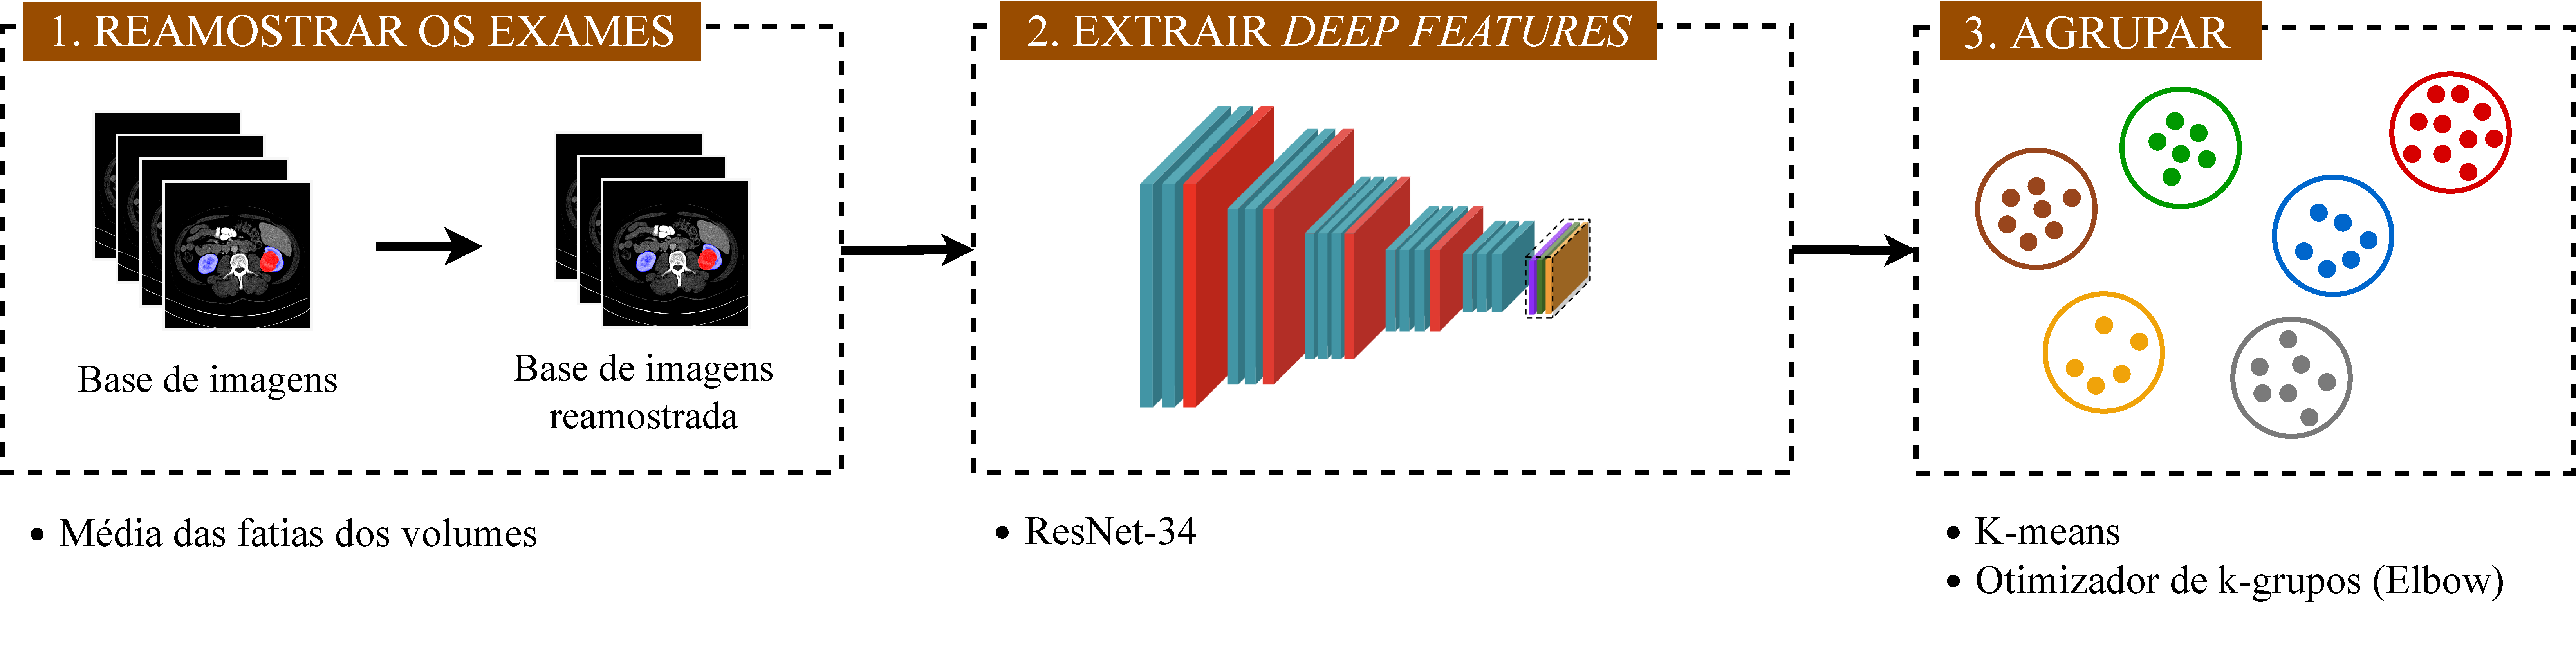
\includegraphics[width=1\textwidth]{figuras/distribuicao-proporcional-automatica.pdf}
    \label{fig:metodo-agrupar}
    \legend{Fonte: Elaborado pela autora.}
\end{figure}

Na primeira etapa, é realizada a técnica de reamostragem~\cite{dodgson1992image, 1372173} das tomografias, que é uma técnica matemática usada para criar uma nova versão da imagem com diferentes larguras, alturas e/ou profundidades em \textit{pixels}~\cite{dodgson1992image,sachs2001image}. Essa etapa é necessária porque os exames de TC podem ter diferentes quantidades de fatias e precisam ser reamostrados para o mesmo número de fatias para que os dados de entrada das etapas consecutivas sejam normalizados. Essa transformação dos dados é uma prática comum para evitar que o algoritmo fique enviesado para as variáveis com maior ordem de grandeza~\cite{kimble2015big}.

Para isso, padroniza-se o número de fatias em cada exame de TC por meio da operação de média, que consiste em calcular a quantidade total de fatias de tumores contidos na base de imagens (conjunto de treino e validação) e dividir pela quantidade de exames totais. Como resultado, obtém-se o valor médio de fatias. Posteriormente, a reamostragem é aplicada aos exames usando a informação do valor médio e interpolação linear, que produz uma superfície de intensidade garantida de forma contínua~\cite{andrews1976digital, dodgson1992image}. Por fim, com a técnica de reamostragem, todos os exames passam a ter um número n de fatias.

Na segunda etapa, são extraídas as \textit{deep features} que servirão como dados de entrada para a próxima etapa. As \textit{deep features} são extraídas pelos modelos ResNet-18, ResNet-34, ResNet-101~\cite{He7780459}, VGG-11, VGG-16~\cite{simonyan2014very}, DPN-131~\cite{chen2017dual} e Xception~\cite{chollet2017xception}. Esses modelos foram escolhidos por estarem consolidados na literatura para essa tarefa~\cite{8875911}, apresentando um alto desempenho, além de já terem sido pré-treinados. Todos os modelos realizam implicitamente a extração e seleção de características da região dos tumores. As características obtidas são extraídas da última camada de convolução de cada arquitetura. Os modelos são inicializados usando pesos pré-treinados aplicados à base de imagens ImageNet~\cite{deng2009imagenet}.

Finalmente, na terceira etapa, as características extraídas por cada modelo são utilizadas individualmente para realizar experimentos relacionados ao agrupamento de dados. O agrupamento é o processo de dividir os dados inteiros em grupos (também conhecidos como \textit{clusters}) com base nos padrões dos dados. Portanto, esta etapa visa agrupar os exames que possuam características semelhantes. Para isso, foi usado o K-means~\cite{macqueen1967some,hamerly2003learning}, que é o algoritmo de agrupamento mais comumente usado na literatura, para dividir o conjunto de dados em um conjunto de K-grupos. No K-means, cada grupo é representado pelo seu centro (isto é, centroide) que corresponde à média dos pontos atribuídos ao grupo. Em geral, as características extraídas de cada exame na segunda etapa são classificadas em grupos, de modo que tenham alta similaridade intraclasse e baixa similaridade interclasse.

Inicialmente, o modelo K-means é parametrizado em cada modelo de rede com diferentes números de K-grupos (de 2 a 20). Para cada valor de K, a inércia é calculada para medir o quão bem um conjunto de dados foi agrupado pelo K-means. A inércia é calculada medindo a distância entre cada ponto de dados e seu centroide, elevando essa distância ao quadrado e somando esses quadrados em um grupo. Posteriormente, o hiperparâmetro K é otimizado com o método do cotovelo (Elbow)~\cite{joshi2013modified}, que é frequentemente usado para encontrar o número ideal de grupos. Na Figura~\ref{fig:metodo-cotovelo} o valor da inércia para cada K associado é ilustrado usando o método do cotovelo. Pode-se observar que à medida que o número de grupos aumenta, o valor da inércia começa a diminuir. Além disso, o gráfico muda rapidamente em um ponto, criando uma forma de cotovelo, a partir do qual o gráfico começa a se mover quase paralelo ao eixo X. O método do cotovelo seleciona esse ponto do cotovelo no gráfico de inércia, pois o valor K correspondente é o valor K ótimo ou um número ótimo de grupos.

\begin{figure}[!ht]
    \centering
    \caption{Exemplo do método do cotovelo para seleção o número ideal de K-grupos.}
    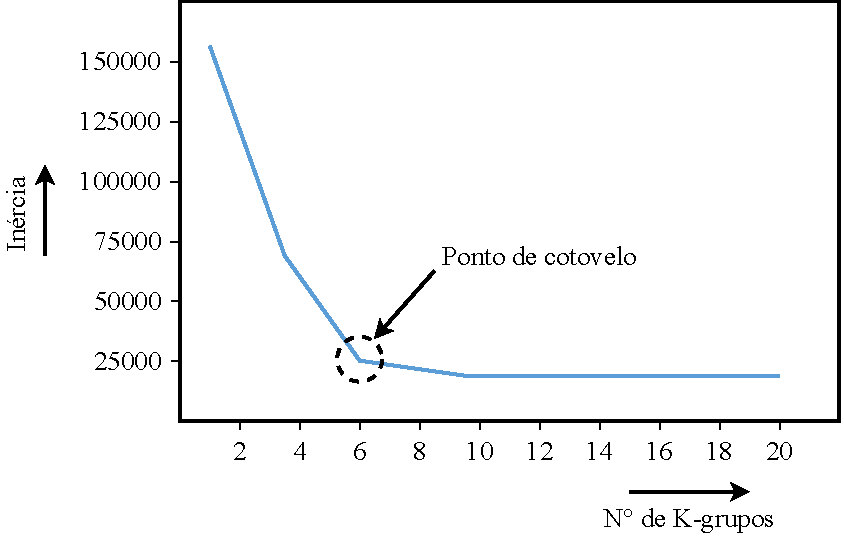
\includegraphics[width=0.75\textwidth]{figuras/metodo-cotovelo.pdf}
    \label{fig:metodo-cotovelo}
    \legend{Fonte: Elaborado pela autora.}
\end{figure}

Sabe-se que a ideia por trás de um bom agrupamento é ter um pequeno valor de inércia e um pequeno número de agrupamentos~\cite{joshi2013modified}. Portanto, este mesmo processo descrito acima é realizado para cada modelo de rede a fim de encontrar o seu melhor grupo. Posteriormente, dentre os modelos, deve-se selecionar aquele com menor valor de inércia, pois representará o modelo com melhor número de grupos. Isso completa o método para agrupar exames semelhantes.

Vale ressaltar que antes de aplicar as etapas descritas, o conjunto de teste é escolhido aleatoriamente da base de imagens. Em sequência, os exames de cada um dos grupos gerados pelo método proposto são selecionados aleatoriamente e distribuídos proporcionalmente entre os conjuntos de dados de treinamento e validação. Isso garante um modelo mais equilibrado, pois deve haver exames de todos os grupos de tumores em ambos os conjuntos de dados. Consequentemente, a generalização do modelo é aumentada.

Depois de distribuir proporcionalmente a base de imagens, alguns outros pré-processamentos foram aplicados para aprimorar as imagens de TC. Conforme já mencionado, esses outros pré-processamentos foram realizados em diferentes fluxos (descrito nas próximas subseções) para cada modelo de segmentação. Posteriormente, as imagens pré-processadas foram aplicadas para segmentar os rins e candidatos a tumores renais.

\subsection{Pré-processamentos Aplicados a Segmentação dos Rins}
\label{sec:pre-processamento-SR}

Antes de treinar o modelo de segmentação dos rins, os exames de TC são inicialmente submetidos a um processo de pré-processamento dividido em duas etapas. Essas etapas são ilustradas na Figura~\ref{fig:especificacao-janelamento}. A primeira etapa (Figura~\ref{fig:especificacao-janelamento} (a)) é a normalização das intensidades dos \textit{voxels} dos volumes de TC uma vez que as mesmas regiões dos rins podem ter intensidades muito diferentes em volumes diferentes, as quais podem dificultar uma eventual comparação das características de textura das regiões renais. Portanto, a especificação do histograma é aplicada para aproximar o histograma de um volume de TC ao histograma de um volume modelo escolhido aleatoriamente (fatia do volume modelo na Figura~\ref{fig:especificacao-janelamento}), de modo que ambos tenham uma distribuição dos \textit{voxels} semelhante~\cite{gonzalez2008digital}.

\begin{figure}[!ht]
    \centering
    \caption{Pré-processamento: (a) especificação do histograma; (b) janelamento.}
    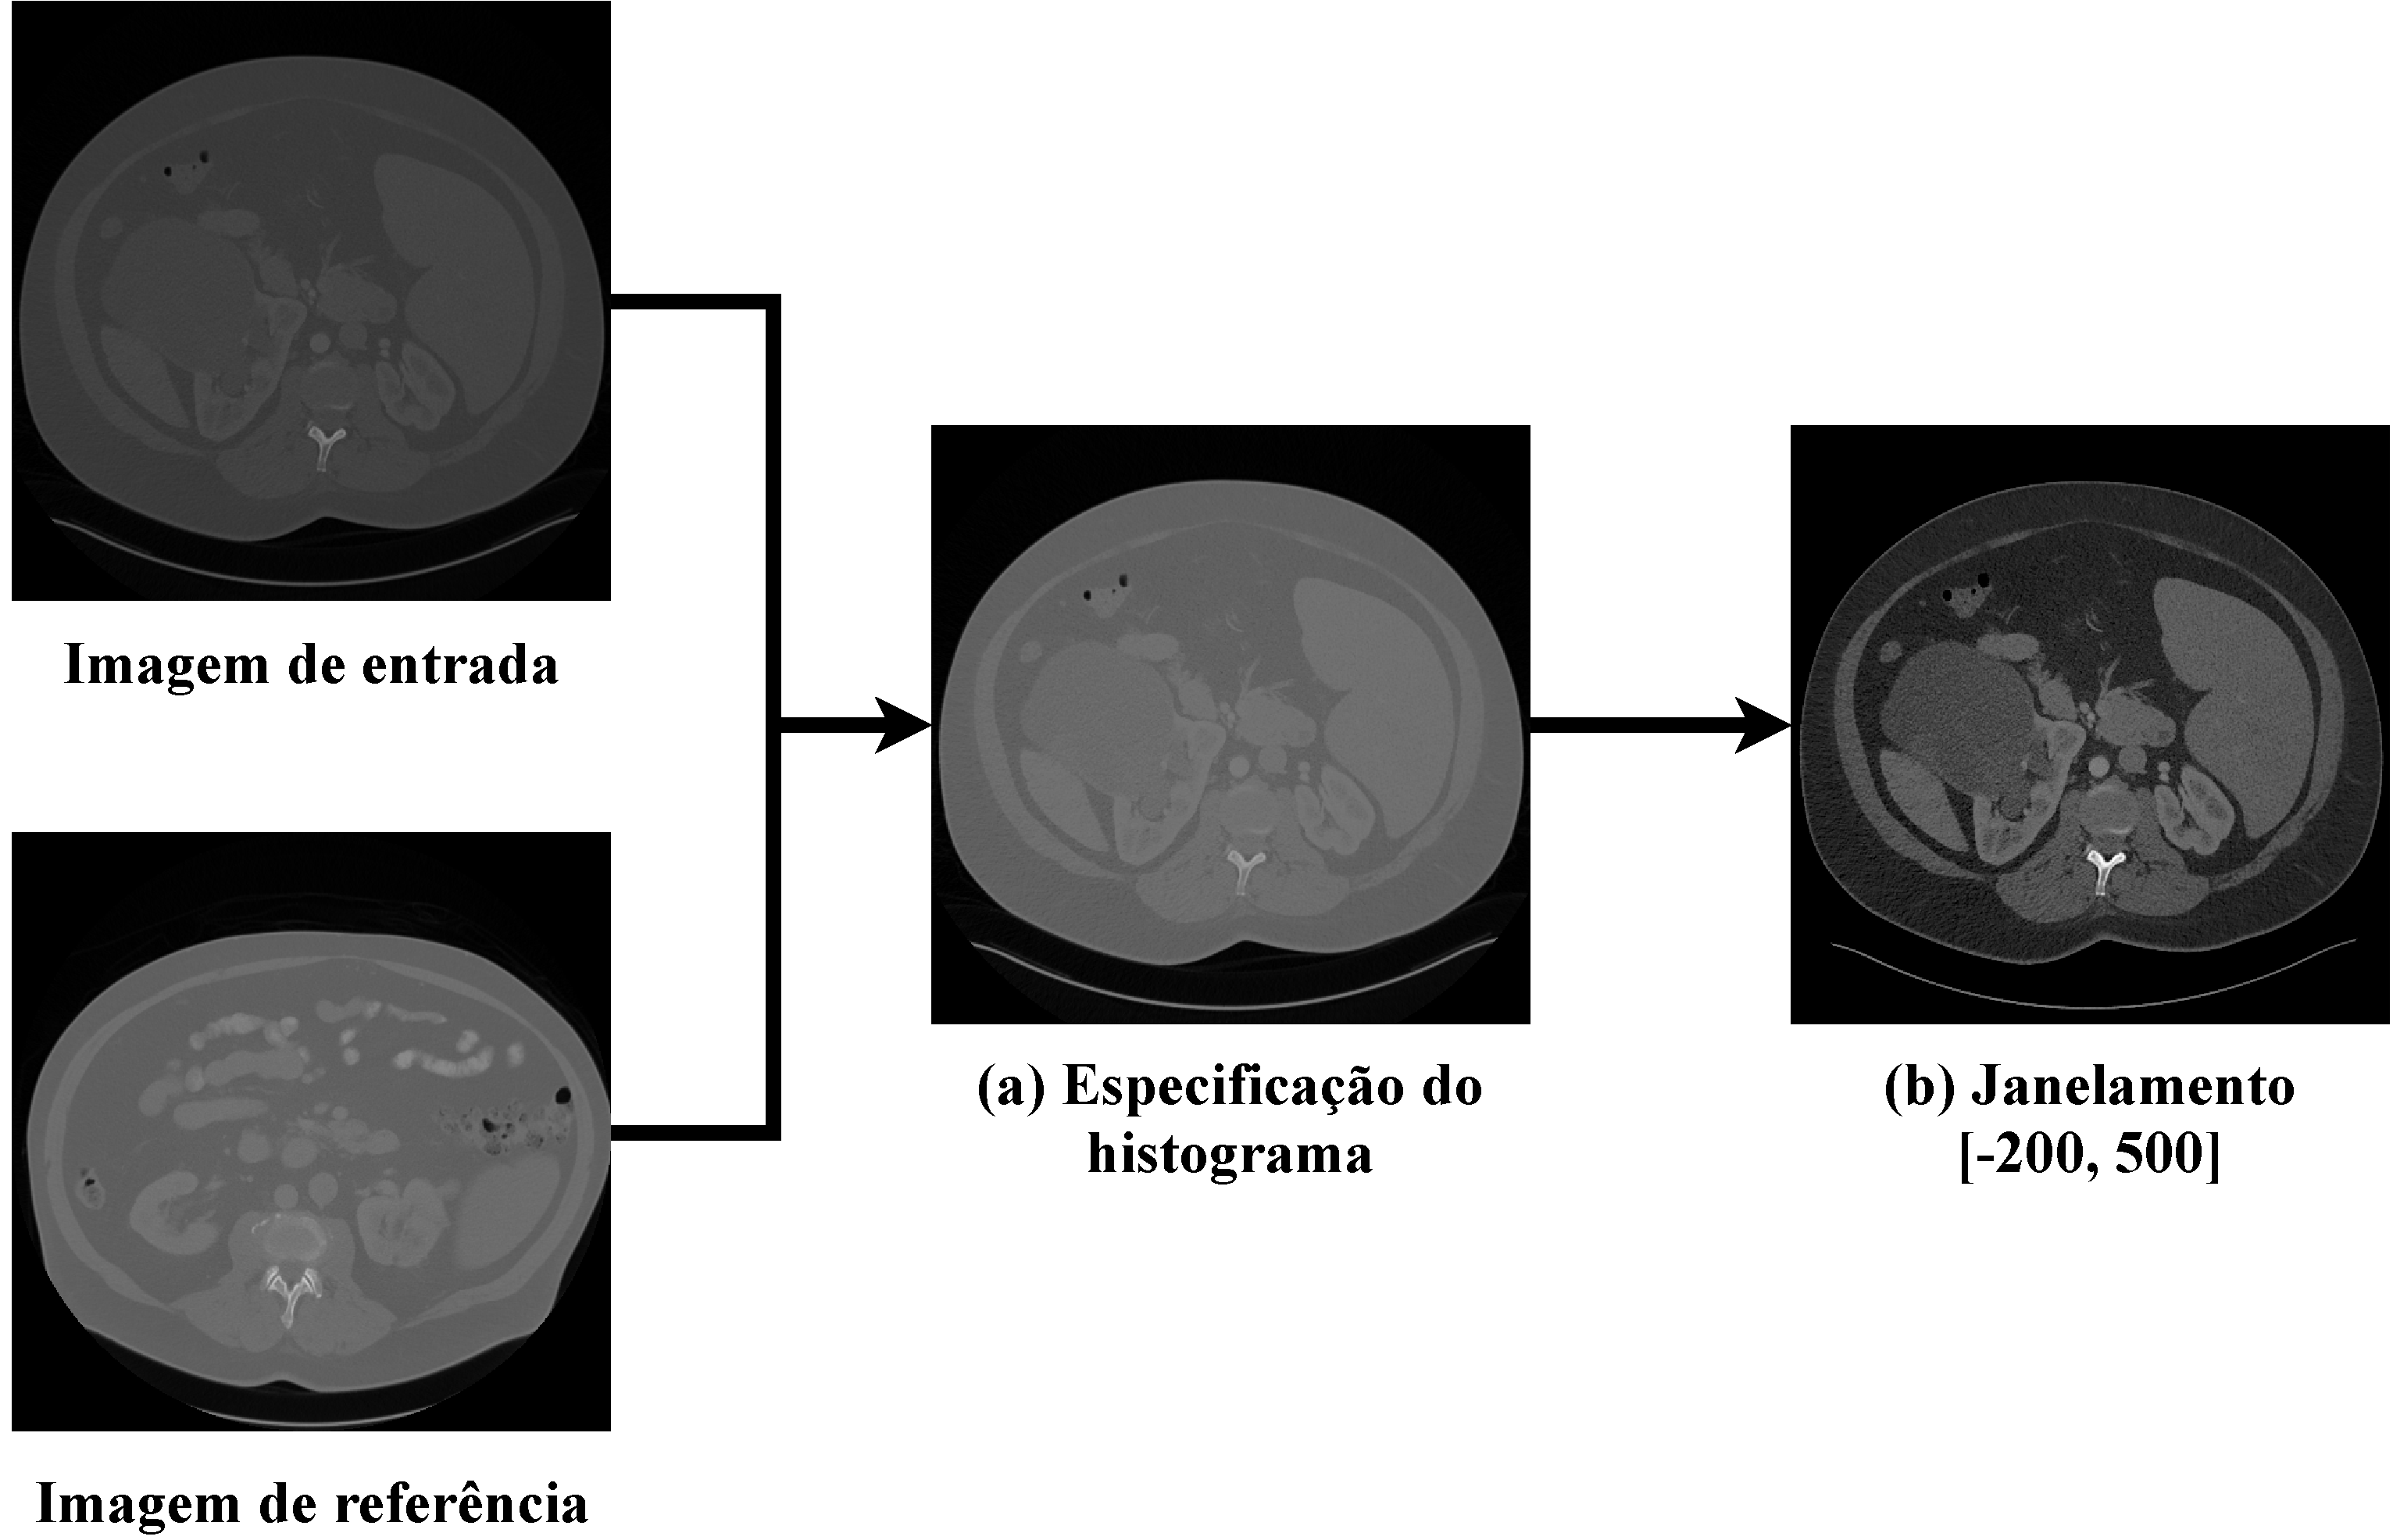
\includegraphics[width=0.85\textwidth]{figuras/especificacao-janelamento.pdf}
    \legend{Fonte: Elaborado pela autora.}
    \label{fig:especificacao-janelamento}
\end{figure}

Devido a existência de ossos, ar no intestino e outros órgãos, a faixa dos valores de TC nas imagens pode variar de -10.240 a mais de 18.000 HU. Valores tomográficos de tecidos moles, como rins e tumores renais, têm a mesma distribuição, variando de aproximadamente -200 HU a 500 HU \cite{Buzug2011, ADAMS2012277, yang2018automatic}. Portanto, na segunda etapa, os valores de intensidades dos volumes foram limitados para a faixa de [-200, 500] HU (Figura~\ref{fig:especificacao-janelamento} (b)). Este processo consiste em um janelamento, no qual se preserva os valores de \textit{voxels} que estão no intervalo entre -200 e 500 HU, e os \textit{voxels} com valores inferiores ou superiores a este intervalo são atribuídos os valores -200 e 500 HU, respectivamente. Isso melhora o contraste das imagens, facilitando a diferenciação das estruturas renais de outros órgãos~\cite{yang2018automatic,da2020kidney}. Em seguida, os valores de intensidade limitados foram normalizados entre 0 e 1. Esta transformação melhora a estabilidade da otimização, reduzindo a influência do problema de explosão de gradiente~\cite{Jason2019, Yash2021}.

\subsection{Pré-processamentos Aplicados à Segmentação Inicial de Candidatos a Tumores Renais}
\label{sec:pre-processamento-SRTR}

Para treinar os modelos de segmentação inicial a candidatos de tumores renais, as imagens de TC foram primeiramente submetidas ao pré-processamento de janelamento [-200, 500], que é o mesmo aplicado na segmentação de rins (Seção~\ref{sec:pre-processamento-SR}). A Figura~\ref{fig:janelamento} ilustra esse processo. Posteriormente, os valores de intensidade limitados com o janelamento também foram normalizados entre 0 e 1~\cite{Hands2017}.

\begin{figure}[!ht]
    \centering
    \caption{Pré-processamento: (a) imagem original; (b) janelamento.}
    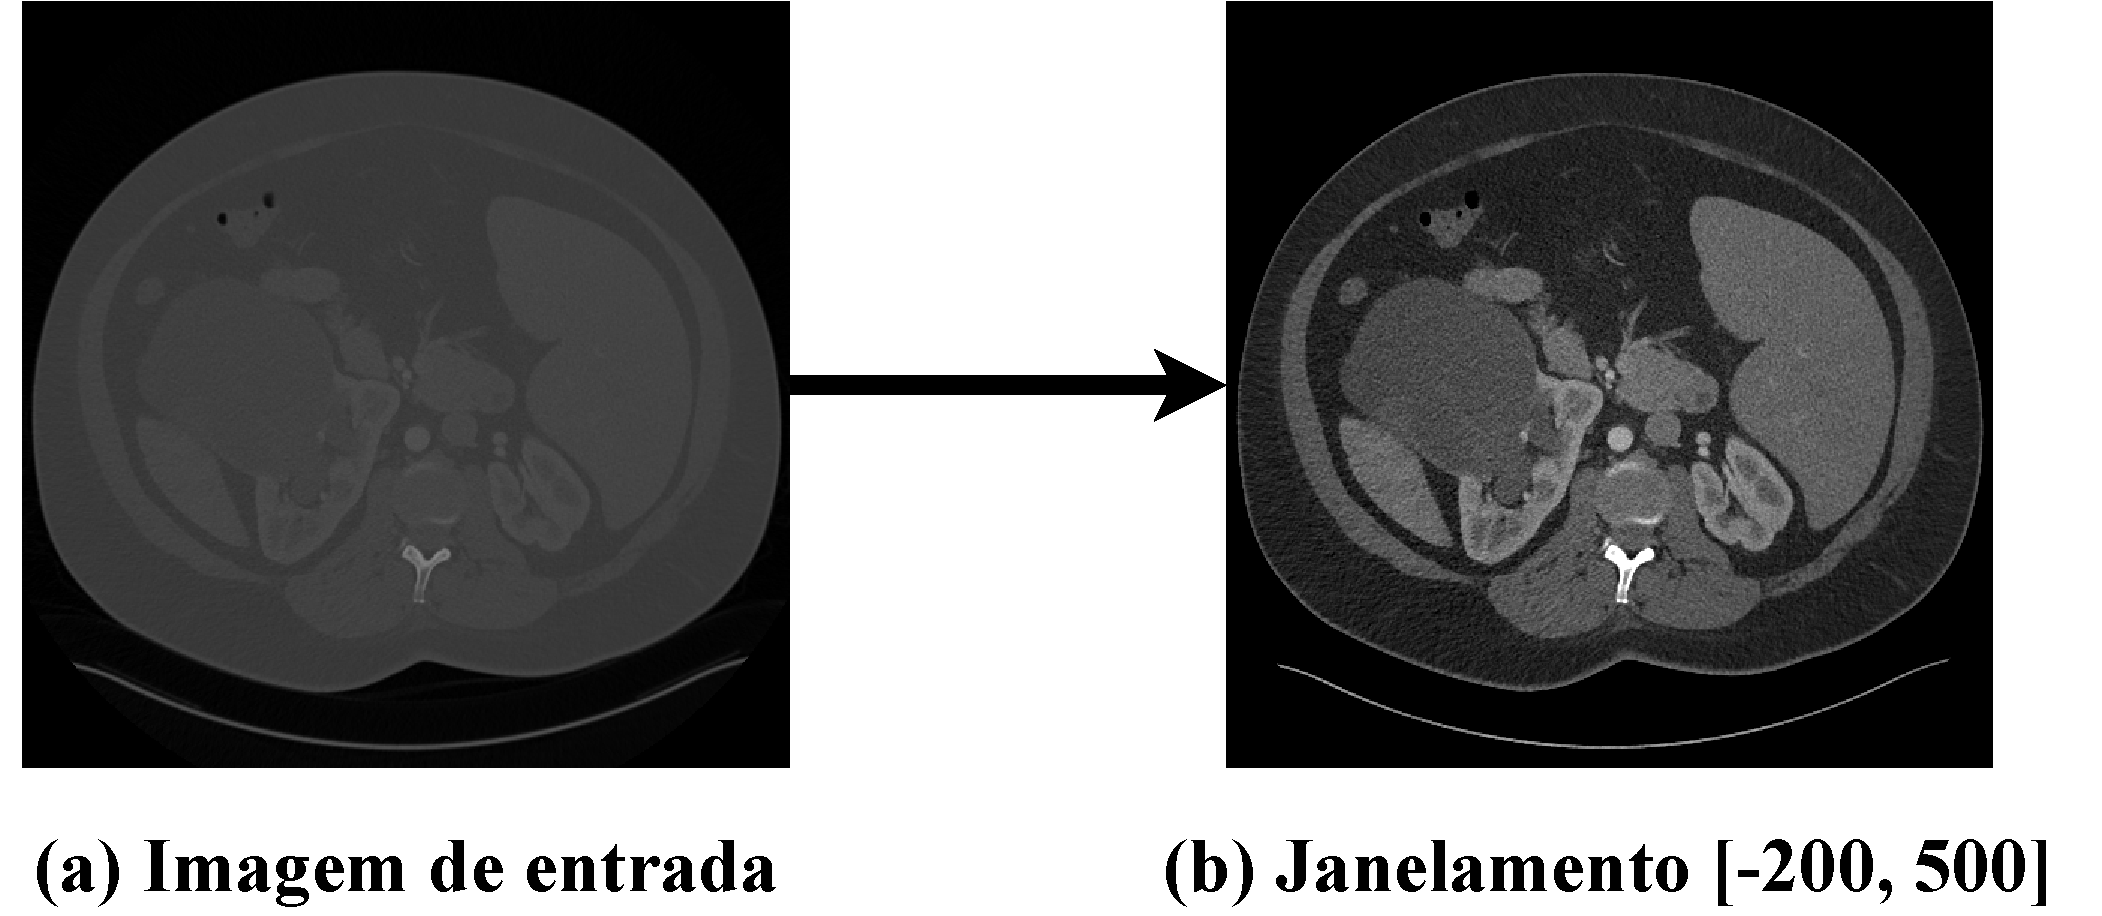
\includegraphics[width=0.75\textwidth]{figuras/janelamento.pdf}
    \legend{Fonte: Elaborado pela autora.}
    \label{fig:janelamento}
\end{figure}

\section{Segmentação Inicial}
\label{sec:metodo-segmentacao-inicial}

%Esta etapa visa a segmentação inicial dos rins e tumores renais após o pré-processamento das imagens de TC. Para isso, foram usados os modelos ResUNet e DeepLabv3+ para segmentar os rins e tumores renais, respectivamente. Após os modelos treinados, o processo de obter as segmentações dos rins e tumores renais ocorre em forma de cascata. Ou seja, os resultados da segmentação dos rins são usados como entrada para segmentar os tumores renais. Nas próximas subseções serão descritos os procedimentos para segmentar os rins e tumores renais.

Esta etapa visa a segmentação inicial dos rins e candidatos a tumores renais. Inicialmente, o modelo ResUNet foi usado para segmentar os rins. Para segmentar os candidatos a tumores renais, foram abordados dois estágios. O primeiro estágio usa o modelo DeepLabv3+ e o segundo estágio usa o modelo ResUNet. Nas próximas subseções serão descritos os procedimentos para segmentar os rins e candidatos a tumores renais.

\subsection{Segmentação dos rins usando a ResUNet}
\label{sec:metodo-segmentacao-dos-rins-ResUNet}

A ResUNet é uma arquitetura desenvolvida por \citeonline{ResUNet_8309343} para segmentação semântica. Foi inicialmente usada para extração de estradas a partir de imagens aéreas, mais tarde usada para várias outras aplicações, como segmentação de tumor cerebral e imagens humanas. Essa arquitetura é inspirada nos pontos fortes dos modelos de aprendizagem residual~\cite{He7780459} e U-Net~\cite{ronneberger2015u}. Em resumo, a rede é construída com unidades residuais e tem arquitetura semelhante à da U-Net. As vantagens deste modelo são duplas: em primeiro lugar, as unidades residuais facilitam o treinamento de redes profundas; em segundo, as ricas conexões de salto dentro da rede podem facilitar a propagação de informações renais, permitindo projetar redes com menos parâmetros e mais desempenho.

%Inicialmente, as fatias empilhadas em 3 canais são inseridas como uma imagem \textit{red-green-blue} (RGB).

A arquitetura ResUNet-101 usada neste trabalho é ilustrada na Figura~\ref{fig:arquitetura_ResUNet}. As imagens de entrada da rede são passadas por uma estrutura composta por três partes: codificação, ponte e decodificação. A primeira parte codifica a imagem de entrada em representações compactas. A última parte recupera as representações para uma segmentação semântica. A parte do meio serve como uma ponte conectando os caminhos de codificação e decodificação.

\begin{figure}[!ht]
    \centering
    \caption{Arquitetura ResUNet-101.}
    \includegraphics[width=1\textwidth]{figuras/arquitetura_ResUNet.png}
    \label{fig:arquitetura_ResUNet}
    \legend{Fonte: Elaborado pela autora.}
\end{figure}

A ResUNet usa unidades residuais como bloco de construção básico em vez de bloco convolucional simples. O caminho de codificação e decodificação é composto por quatro unidades residuais. As três partes são construídas com unidades residuais que consistem em dois blocos de convolução $3\times3$ e um mapeamento de identidade. Cada bloco de convolução inclui uma camada \textit{batch normalization}, uma camada de ativação ReLU e uma camada convolucional. O mapeamento de identidade conecta (adição) a entrada e a saída da unidade. No caminho de decodificação, antes de cada unidade, há uma deconvolução de mapas de características de nível inferior e uma concatenação com os mapas de características do caminho de codificação correspondente. Após o último nível do caminho de decodificação, uma convolução $1\times1$ e uma camada de ativação sigmoide são usadas para projetar os mapas de características para a segmentação dos rins.

Resumidamente, a abordagem residual consiste em propagar informações sobre camadas, inserindo conexões de atalho entre as camadas de entrada e saída. Essas conexões de atalho simplesmente executam o mapeamento de identidade e suas saídas são adicionadas às saídas das camadas empilhadas. Assim, a inserção dos mapas de entrada na saída de cada camada evita que o conjunto de operações de \textit{pooling} reduza as informações necessárias contidas nas imagens da base. Portanto, este modelo foi escolhido devido ao seu alto desempenho para segmentação renal, uma vez que as informações são propagadas com a abordagem residual, retendo e agregando características renais relevantes.

%Os blocos residuais criam um mapeamento de identidade para ativações anteriores na rede para impedir o problema de degradação de desempenho associado a arquiteturas neurais profundas.
%No entanto, ResNets profundos são capazes de formar uma função de identidade que mapeia para uma ativação anterior na rede quando a ativação de uma camada específica tende a zerar mais profundamente na rede.
%A melhoria do desempenho é alcançada sempre que as camadas extras aprendem algumas informações significativas dos dados. Enquanto, a presença de blocos residuais evita a perda de desempenho sempre que as ativações tendem a desaparecer ou explodir.

%quando combinado com DeepLabv3 + 2.5D, permitiu a exploração de novos recursos, que possibilitaram o aprendizado de representações tumorais a partir da captura de suas informações contextuais, como diferentes formas e tamanhos.

\subsubsection{Treinamento da ResUNet 2.5D}
\label{sec:treinamento-ResUNet}

A rede é treinada com imagens de TC no tamanho original de $512\times512$ \textit{pixels}. O modelo usa uma abordagens 2.5D, que consiste em passar como entrada da rede uma pilha de três fatias consecutivas (anterior, central e posterior) e a máscara referente à fatia central com as marcações dos rins. Para analisar todo o volume de TC, o mesmo processo descrito foi realizado deslizando uma janela de tamanho $3\times3$ com um passo igual a 1 sobre as fatias. A saída da ResUNet é a máscara para a segmentação da fatia central da pilha. Um exemplo de fatias de entrada da rede usando a abordagem 2.5D é mostrado na Figura~\ref{fig:abordagem-2.5D}.

%Posteriormente, as segmentações de cada fatia são combinadas para construir o volume 3D do resultado de cada caso no conjunto de dados da tese.

\begin{figure}[!ht]
    \centering
    \caption{Abordagem 2.5D: exemplo de imagens de entrada.}
    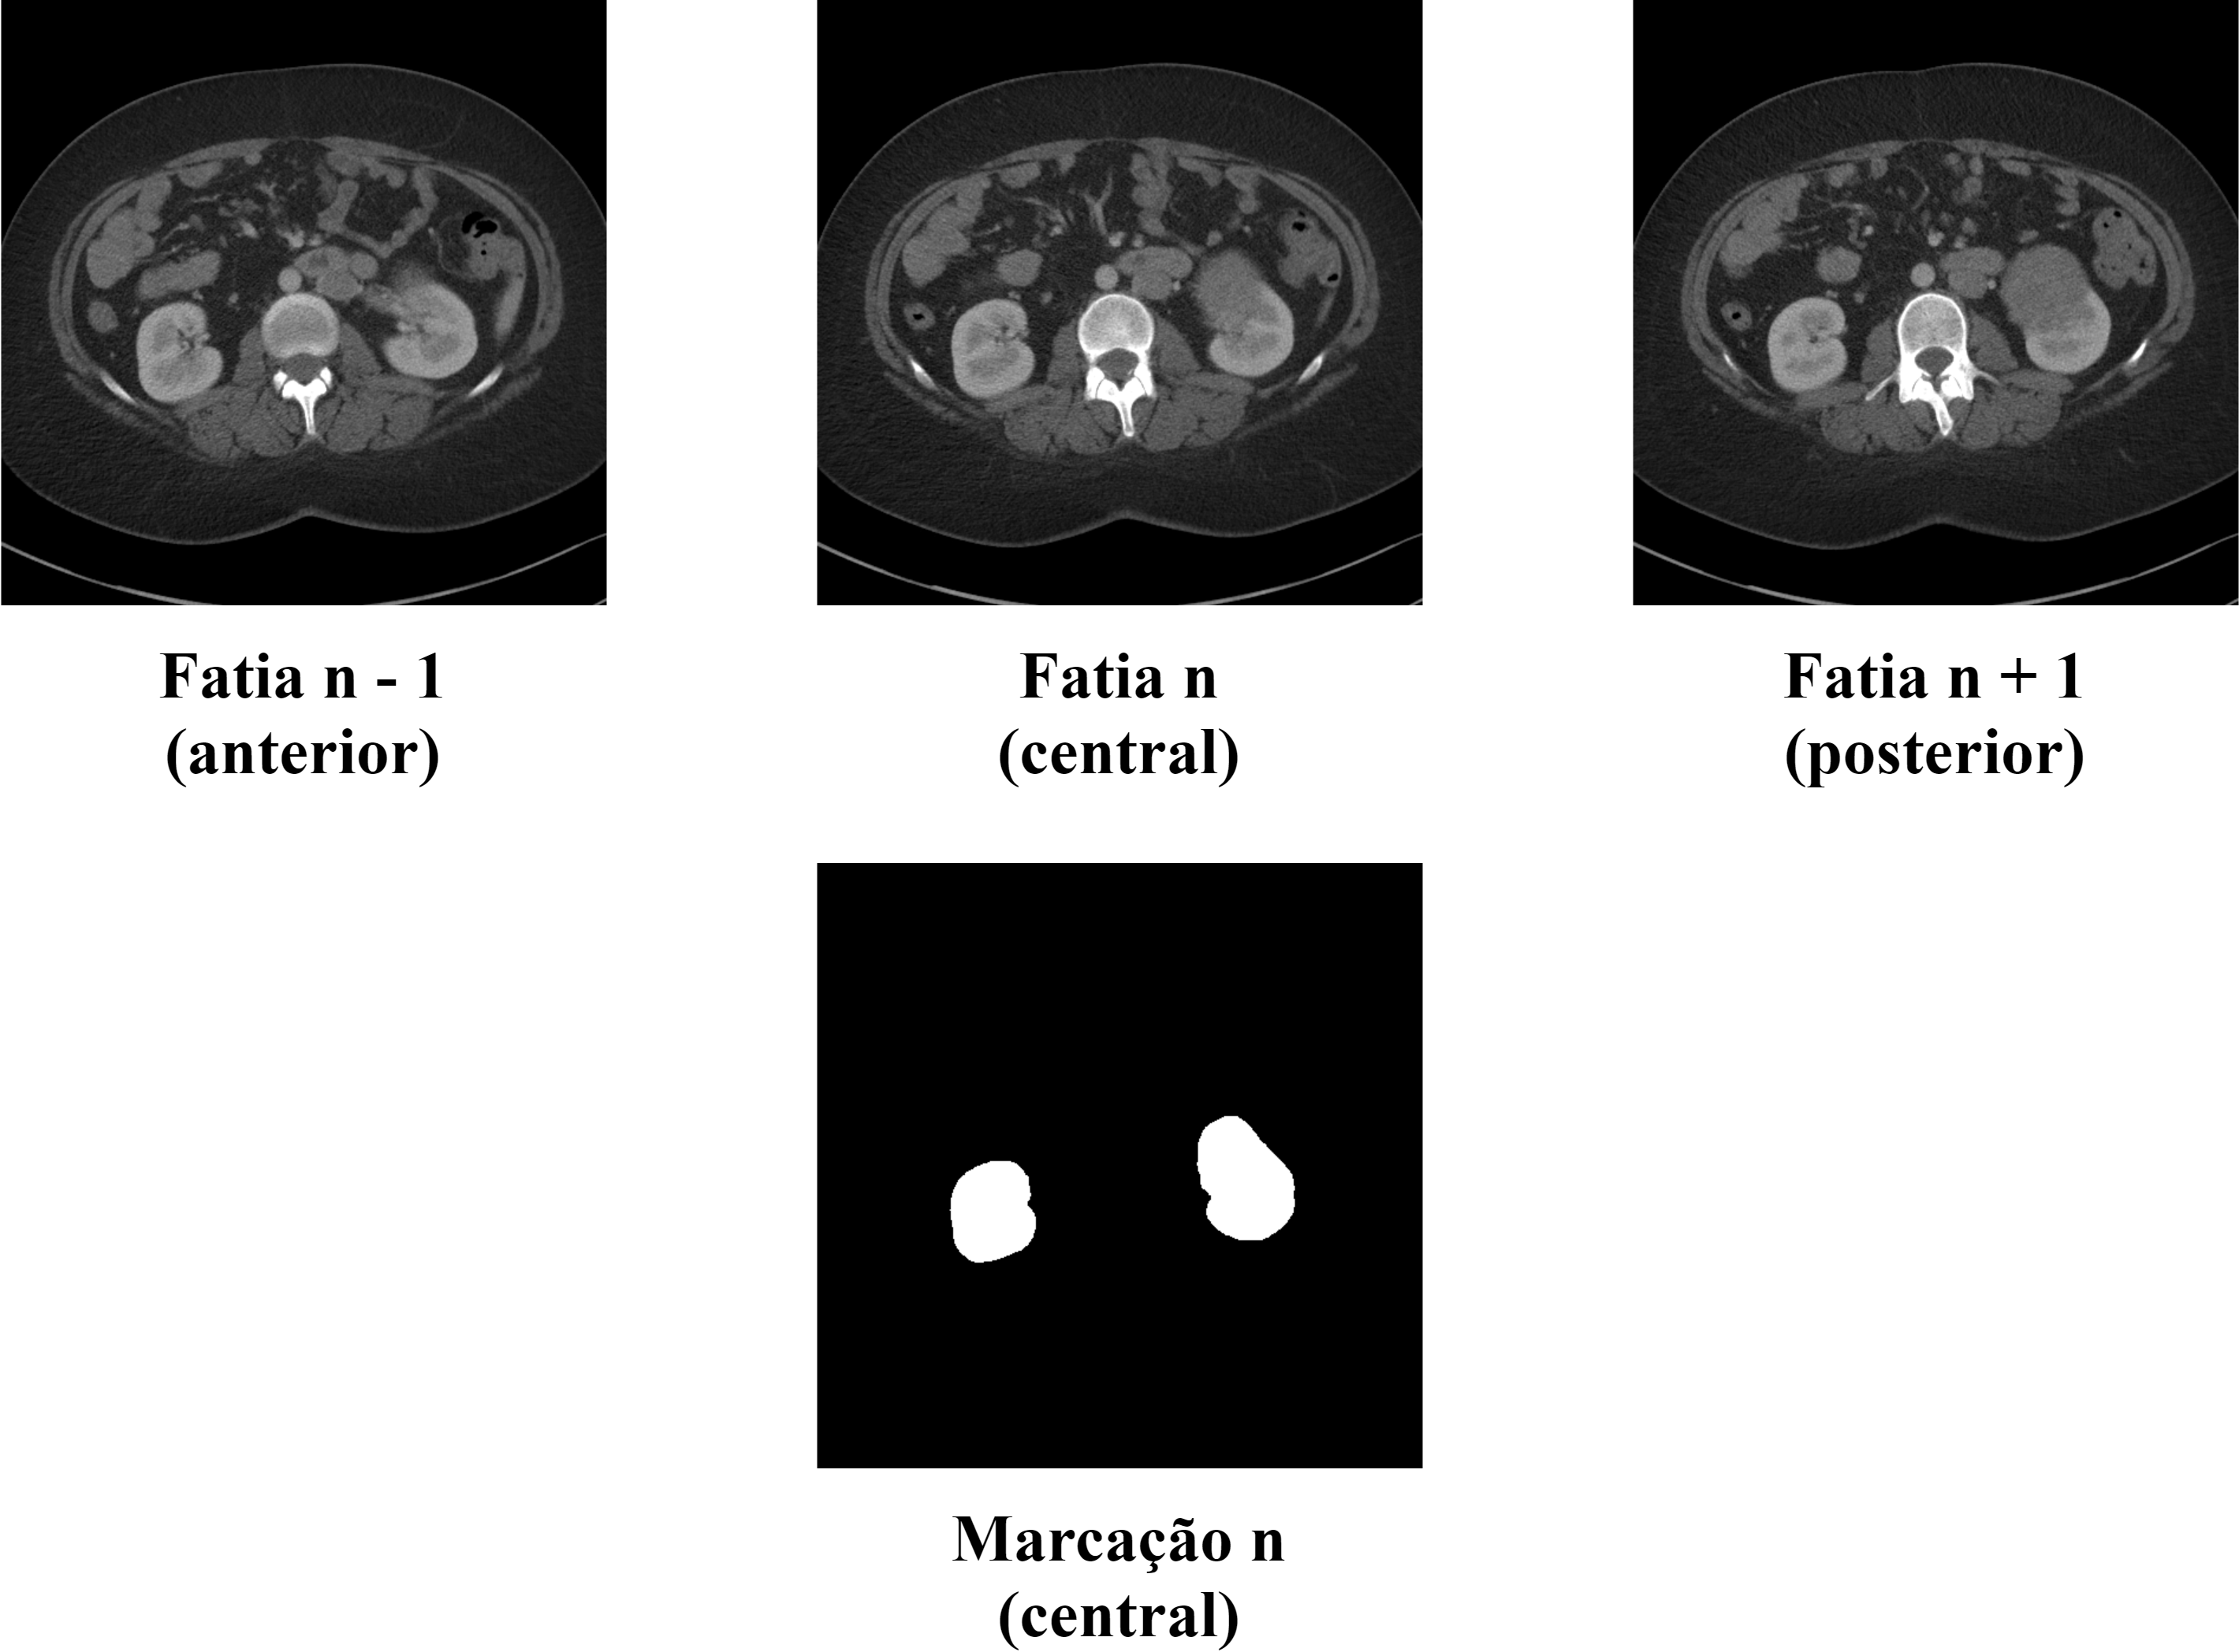
\includegraphics[width=0.8\textwidth]{figuras/abordagem-2.5D-entrada.png}
    \label{fig:abordagem-2.5D}
    \legend{Fonte: Elaborado pela autora.}
\end{figure}

Uma das vantagens da abordagem 2.5D é que pode-se usar informações espaciais das fatias vizinhas para identificar o objeto de interesse, aumentando as chances de segmentação bem-sucedida e reduzindo os falsos positivos. Isso só foi possível devido à natureza da abordagem 2.5D, que possui conexões entre as fatias do volume de TC. 

Além da abordagem 2.5D, um balanceamento de fatias de rins e não rins foi usado nos conjuntos de treinamento e validação. O balanceamento consistiu em usar as fatias com rins e adicionar a mesma quantidade de fatias sem rins e depois retirar o excesso de fatias sem rins. Essa estratégia ajuda o modelo de aprendizado profundo a detectar se uma fatia tem rins ou não, a qual reduziu consideravelmente os falsos positivos.

%o que foi equivalente a 28.732 imagens (14.366 com rins e 14.366 sem rins) e as fatias em excesso sem rins foram removidas (11.186 fatias)

Por fim, o treinamento da ResUNet 2.5D foi inicializado usando os pesos pré-treinados aplicados à base de imagens ImageNet~\cite{deng2009imagenet}. Essa prática ajuda a minimizar o tempo de treinamento e economizar recursos de \textit{hardware}.

\subsection{Segmentação Inicial de Candidatos a Tumores Renais}
\label{sec:metodo-segmentacao-inicial-candidatos-tumores-renais}

Esta etapa visa a segmentação inicial de candidatos a tumores renais. Para isso, foi dividida em dois estágios: o primeiro estágio usa os resultados da segmentação inicial dos rins como entrada para segmentar os candidatos a tumores renais usando o modelo DeepLabv3+; o segundo estágio usa outro modelo ResUNet para segmentar candidatos a tumores renais dentro da região abdominal (imagem completa). Mais detalhes de cada estágio são descritos nas próximas subseções.

\subsubsection{Candidatos de Tumores Renais na Região Renal}
\label{sec:metodo-candidatos-tumores-renais-regiao-renal}

Como já mencionado, este primeiro estágio visa obter candidatos a tumores renais dentro da região renal. Para isso, os resultados adquiridos na etapa de segmentação de rins foram usados como entrada para segmentar os candidatos a tumores renais. Neste estágio, o modelo de aprendizado profundo DeepLabv3+ (Seção~\ref{sec:deeplabv3+}) foi adaptado para realizar a segmentação das regiões tumorais. Esta adaptação consiste em remover o codificador padrão (Xception~\cite{chollet2017xception}) da DeepLabv3+, pela arquitetura de rede de caminho duplo (\textit{Dual Path Network} - DPN)-131. Para isso, foi necessário remover a camada totalmente conectada da DPN-131 para funcionar como um extrator de características no modelo proposto.

A DPN é uma rede de classificação que apresenta uma topologia de caminhos de conexão interna. A DPN compartilha as vantagens da Rede Residual (\textit{Residual Network} - ResNet)~\cite{He7780459}, que permite a reutilização de recursos, e da Rede Densamente Convolucional (\textit{Densely Convolutional Network} - DenseNet)~\cite{Huang8099726}, que explora os novos recursos que são importantes para o aprendizado de boas representações~\cite{chen2017dual}. A DPN-131 empilha vários blocos \textit{dual path} modularizados, conforme mostrado na Figura~\ref{fig:arquitetura_DPN}. Inicialmente, uma convolução 7 × 7 é aplicada, seguida de \textit{batch normalization}, função de ativação ReLU e \textit{max-pooling} $3\times3$. A estrutura de cada bloco é projetada com um estilo de gargalo~\cite{He7780459}, que começa com uma camada convolucional $1\times1$, seguida por uma $3\times3$ e finalizando com uma $1\times1$.

Assim, a saída da última camada convolucional $1\times1$ é dividida em duas partes. Na primeira parte, é adicionado ao caminho residual e, na segunda parte, é concatenado com o caminho densamente conectado. Em outras palavras, as redes residuais adicionam os recursos de entrada aos recursos de saída por meio do caminho residual, e as redes densas usam um caminho densamente conectado para concatenar recursos de entrada com recursos de saída, permitindo que cada bloco receba informações de todos os blocos anteriores. A camada de convolução agrupada na segunda camada é usada como ResNeXt~\cite{xie2017aggregated}, aumentando a capacidade de aprendizado de cada bloco.

\begin{figure}[!ht]
    \centering
    \caption{Arquitetura DPN-131.}
    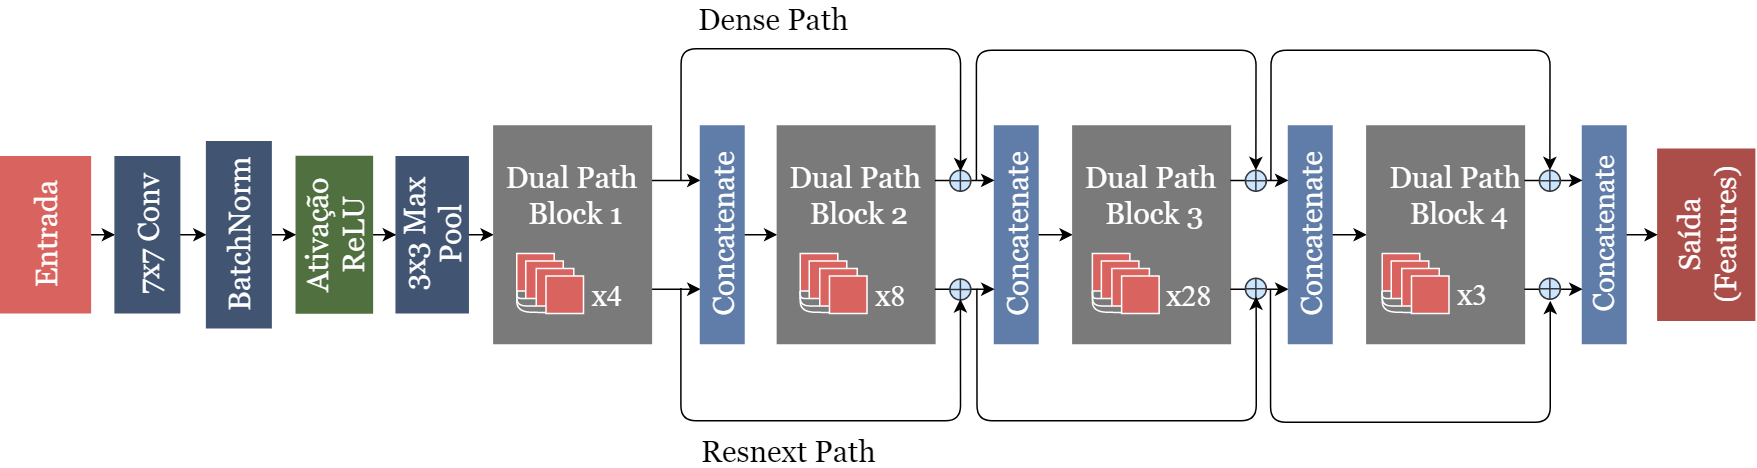
\includegraphics[width=1\textwidth]{figuras/arquitetura_DPN.png}
    \legend{Fonte: Elaborado pela autora.}
    \label{fig:arquitetura_DPN}
\end{figure}

Como a arquitetura DPN-131 padrão foi usada como o codificador da DeepLabv3+, foi necessário remover a camada totalmente conectada do DPN-131 para funcionar como um extrator de características, conforme visto na Figura~\ref{fig:arquitetura_DPN}. Além disso, embora várias funções de ativação tenham sido aplicadas com redes profundas para obter alto desempenho~\cite{8936083, GOCERI2021104118}, foi usada a função ReLU devido à sua eficiência na segmentação da base de imagens e baixo custo computacional.

Finalmente, pode ser observado na Figura~\ref{fig:arquitetura_DeepLabv3+DPN} a arquitetura DeepLabv3+ usada para a segmentação a candidatos de tumores renais. A escolha da DPN-131 foi feita por ser eficiente, introduzindo uma nova topologia de caminhos de conexão internamente. Além disso, vale ressaltar que a DeepLabv3+ é um modelo de aprendizado profundo de última geração capaz de refinar os resultados da segmentação com foco especial nos limites do objeto. Outro ponto importante é que a rede extrai mapas de características densos para capturar contextos de longo alcance (informações contextuais de pixels mais distantes), melhorando a tarefa de segmentar os diferentes tamanhos e formas dos tumores encontrados na base de imagens. Portanto, a combinação resultou em um codificador-decodificador robusto, com alto desempenho para segmentação a candidatos de tumores renais.

\begin{figure}[!ht]
    \centering
    \caption{Arquitetura DeepLabv3+.}
    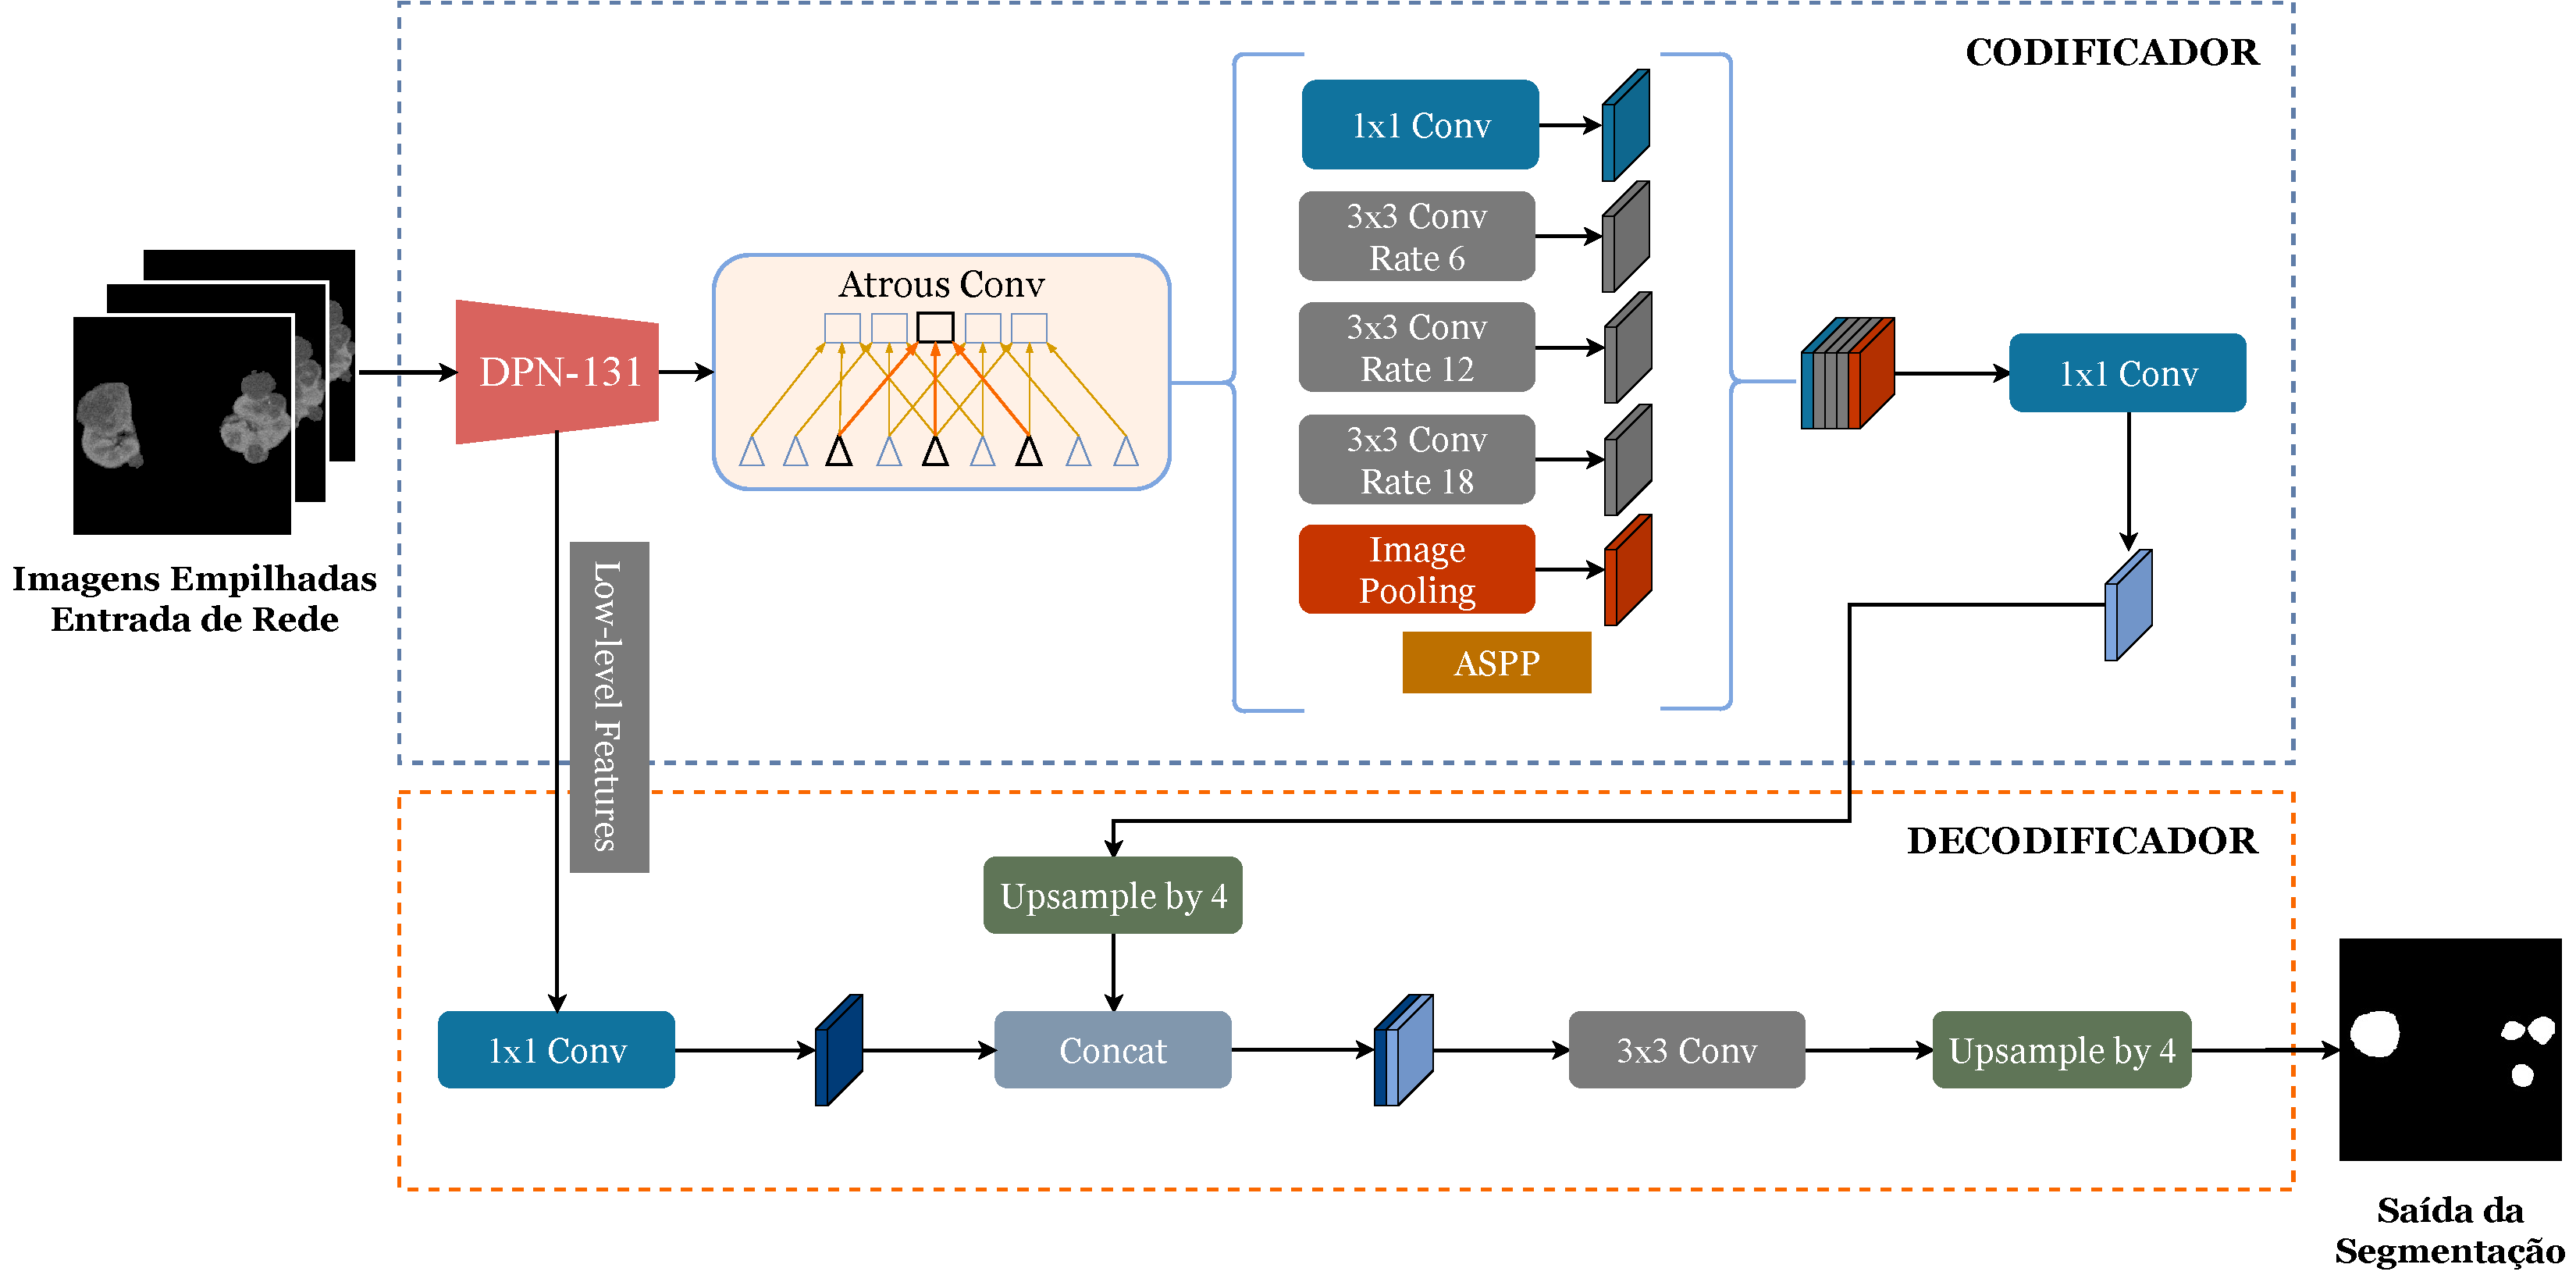
\includegraphics[width=1\textwidth]{figuras/arquitetura_Deeplabv3+DPN.pdf}
    \label{fig:arquitetura_DeepLabv3+DPN}
    \legend{Fonte: Adaptado de~\cite{chen2018encoder}.}
\end{figure}

\subsubsubsection{Treinamento da DeepLabv3+ 2.5D}
\label{sec:treinamento-DeepLabv3+}

Antes de realizar o treinamento, as regiões renais foram inicialmente recortadas automaticamente nas imagens de TC. Os rins foram encontrados usando a marcação do especialista e aplicando uma caixa delimitadora 3D que envolvesse os dois rins (Figura~\ref{fig:recorte} (a)). Então, o volume é cortado para o valor correspondente à caixa delimitadora 3D (Figura~\ref{fig:recorte} (b)). Posteriormente, um redimensionamento proporcional para $256\times256$ \textit{pixels} foi aplicado às imagens cortadas maiores que 256 \textit{pixels} de altura ou largura (Figura~\ref{fig:recorte} (c)). Finalmente, as imagens foram centralizadas com um tamanho final de $256\times256$ \textit{pixels} e apenas a textura da região do rim é mantida (Figura~\ref{fig:recorte} (d)) para a segmentação da região dos tumores. Todo esse processo foi realizado porque havia muitas regiões irrelevantes (outros órgãos) para capturar características. Também foi necessário devido às limitações de \textit{hardware}, já que a arquitetura é profunda e requer memória considerável para representar todos os mapas de características.

\begin{figure}[!ht]
    \centering
    \caption{Delimitação da região de interesse.}
    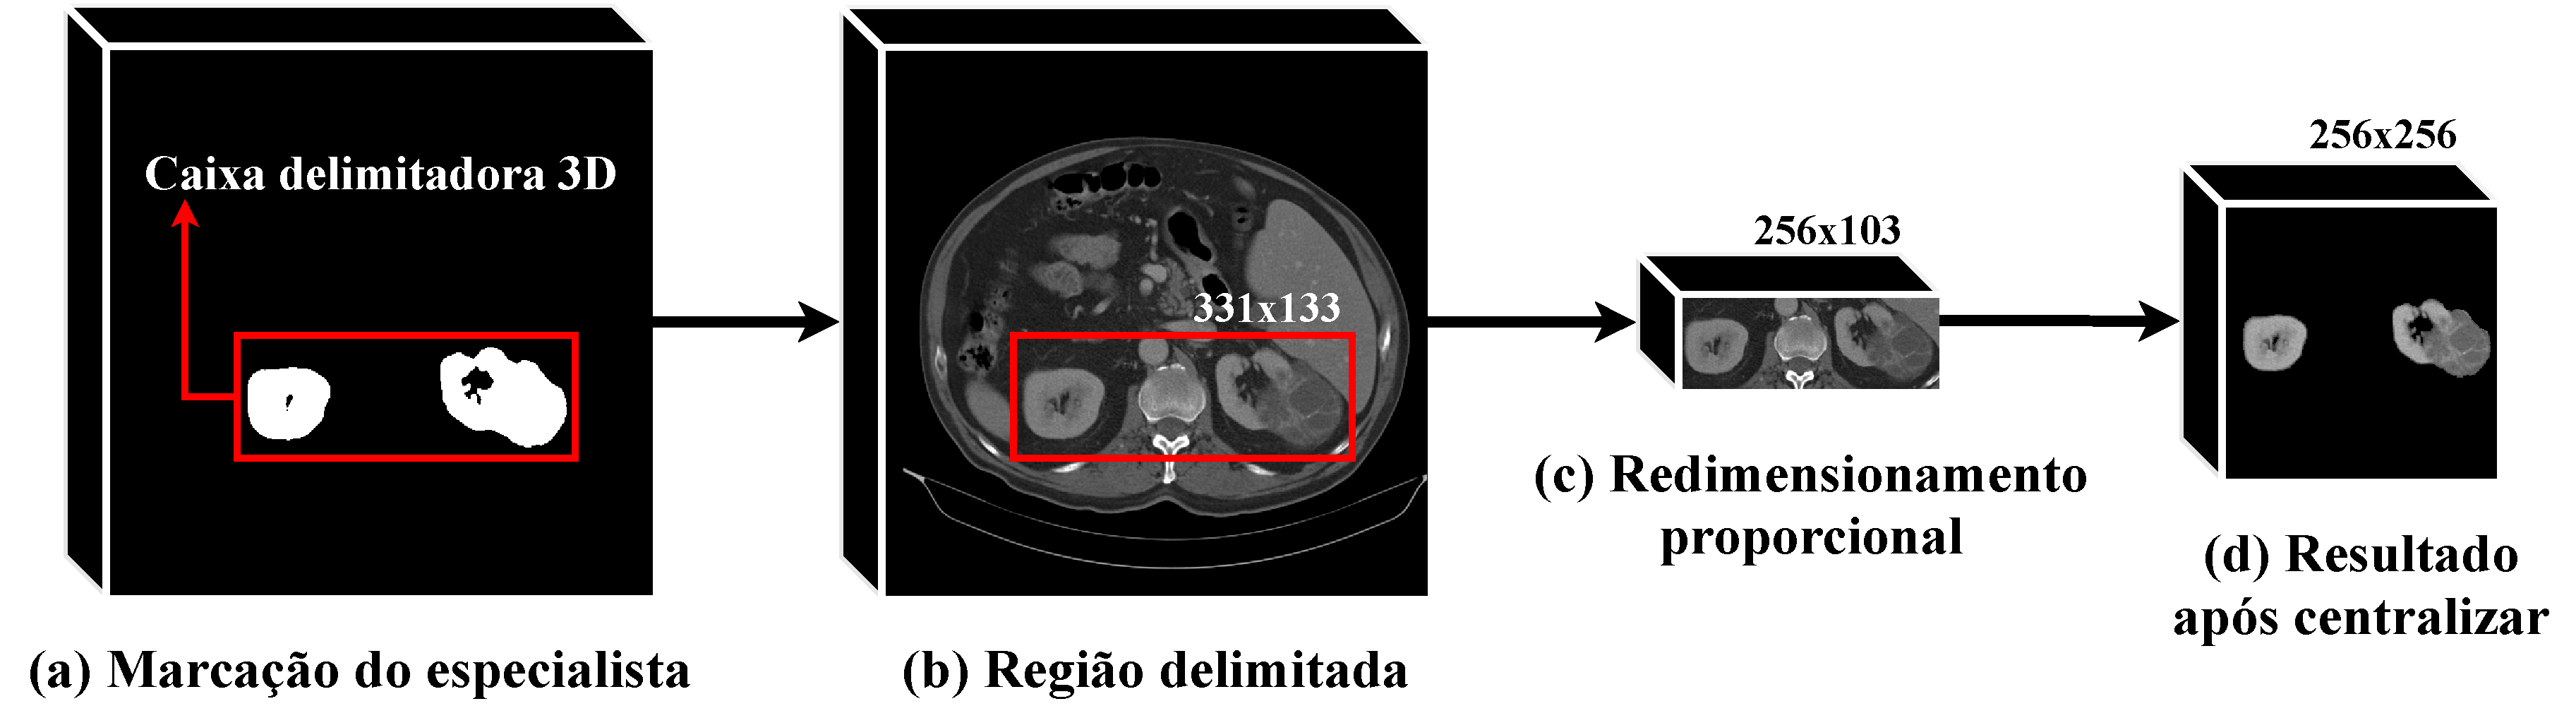
\includegraphics[width=1\textwidth]{figuras/recorte.pdf}
    \legend{Fonte: Elaborado pela autora.}
    \label{fig:recorte}
\end{figure}

Finalmente, o modelo DeepLabv3+ foi treinado usando abordagem 2.5D, conforme descrito na Seção~\ref{sec:treinamento-ResUNet}. No entanto, foram passadas para entrada da rede três fatias consecutivas da região dos tumores e a máscara referente a fatia central com as marcações dos tumores.

Nos experimentos realizados também aplicou-se o balanceamento de fatias (Seção~\ref{sec:treinamento-ResUNet}) nos conjuntos de treinamento e validação. Entretanto, o balanceamento de fatias para o modelo de segmentação a candidatos de tumores renais na região renal consistiu em usar as fatias com tumores e somar a mesma quantidade de fatias sem tumores e, posteriormente, remover as fatias excedentes sem tumores. Isso reduziu bastante os falsos positivos, devido às regiões que são muito semelhantes a tumores renais, como cistos.

%totalizando 9.814 imagens (4.907 com tumores renais e 4.907 sem tumores renais), e as fatias excedentes sem tumores renais foram removidas (4.552 fatias)

A inicialização do treinamento da DeepLabv3+ 2.5D também utilizou os pesos pré-treinados aplicados à base de imagens ImageNet~\cite{deng2009imagenet}.

%A entrada da rede, são fatias de TC empilhadas em 3 canais (RGB). Em seguida, as imagens passam por uma estrutura de codificador-decodificador.

\subsubsection{Candidatos de Tumores Renais na Região Abdominal}
\label{sec:metodo-candidatos-tumores-renais-regiao-abdominal}

O segundo estágio também visa segmentar candidatos a tumores renais. No entanto, toda a região abdominal é analisada. Isso é feito porque no primeiro estágio o modelo está limitado a segmentar candidatos a tumores renais apenas dentro da região renal resultante da segmentação inicial dos rins. Esse procedimento pode acabar não trazendo os resultados desejados por falta de informações contextuais e porque algumas regiões renais não foram obtidas na segmentação inicial dos rins. Logo, essas regiões poderiam ter tumores renais e acabaram não tendo a possibilidade de segmentá-los.

Portanto, o segundo estágio tem o objetivo de segmentar os candidatos a tumores renais na região abdominal, analisando mais informações contextuais em uma região mais ampla. Vale ressaltar que essa técnica é mais suscetível a falsos positivos, pois o tumor renal não tem um formato padronizado, o que pode causar confusão com outras estruturas (órgãos). Entretanto, o modelo traz resultados interessantes, pois é capaz de segmentar tumores renais que não haviam sido segmentados no estágio anterior.

Dessa forma, um segundo modelo de aprendizado profundo é treinado para realizar a segmentação de candidatos a tumores renais na região abdominal. Para isso, é usado o modelo ResUNet que é a mesma arquitetura descrita na Seção~\ref{sec:metodo-segmentacao-dos-rins-ResUNet}. No entanto, o treinamento do modelo é realizado usando apenas as marcações dos tumores renais, mas com informações mais ampla (regiões abdominais). Ou seja, o modelo é especializado nas segmentações dos tumores nas imagens de TC. Além disso, o modelo também usa a abordagem 2.5D e balanceamento de fatias (Seção~\ref{sec:treinamento-DeepLabv3+}). 

A Figura~\ref{fig:candidatos-de-tumores-renais} ilustra a segmentação inicial dos candidatos a tumores renais em uma imagem de TC aplicada à entrada dos modelos (DeepLabv3+ e ResUNet). Na Figura~\ref{fig:candidatos-de-tumores-renais}~(a) apresenta a marcação do especialista. O resultado da etapa de candidatos a tumores renais na região renal é mostrado na Figura~\ref{fig:candidatos-de-tumores-renais} (b). Finalmente, os candidatos a tumores renais na região abdominal que podem não ter sido segmentados no primeiro estágio são ilustrados na Figura~\ref{fig:candidatos-de-tumores-renais} (c). No entanto, nota-se que alguns fragmentos semelhantes a tumores renais também foram segmentados.

\begin{figure}[!ht]
    \centering
    \caption{Candidatos a tumores renais: (a) marcação do especialista; (b) candidatos de tumores renais na região renal; (c) candidatos de tumores renais na região abdominal.}
    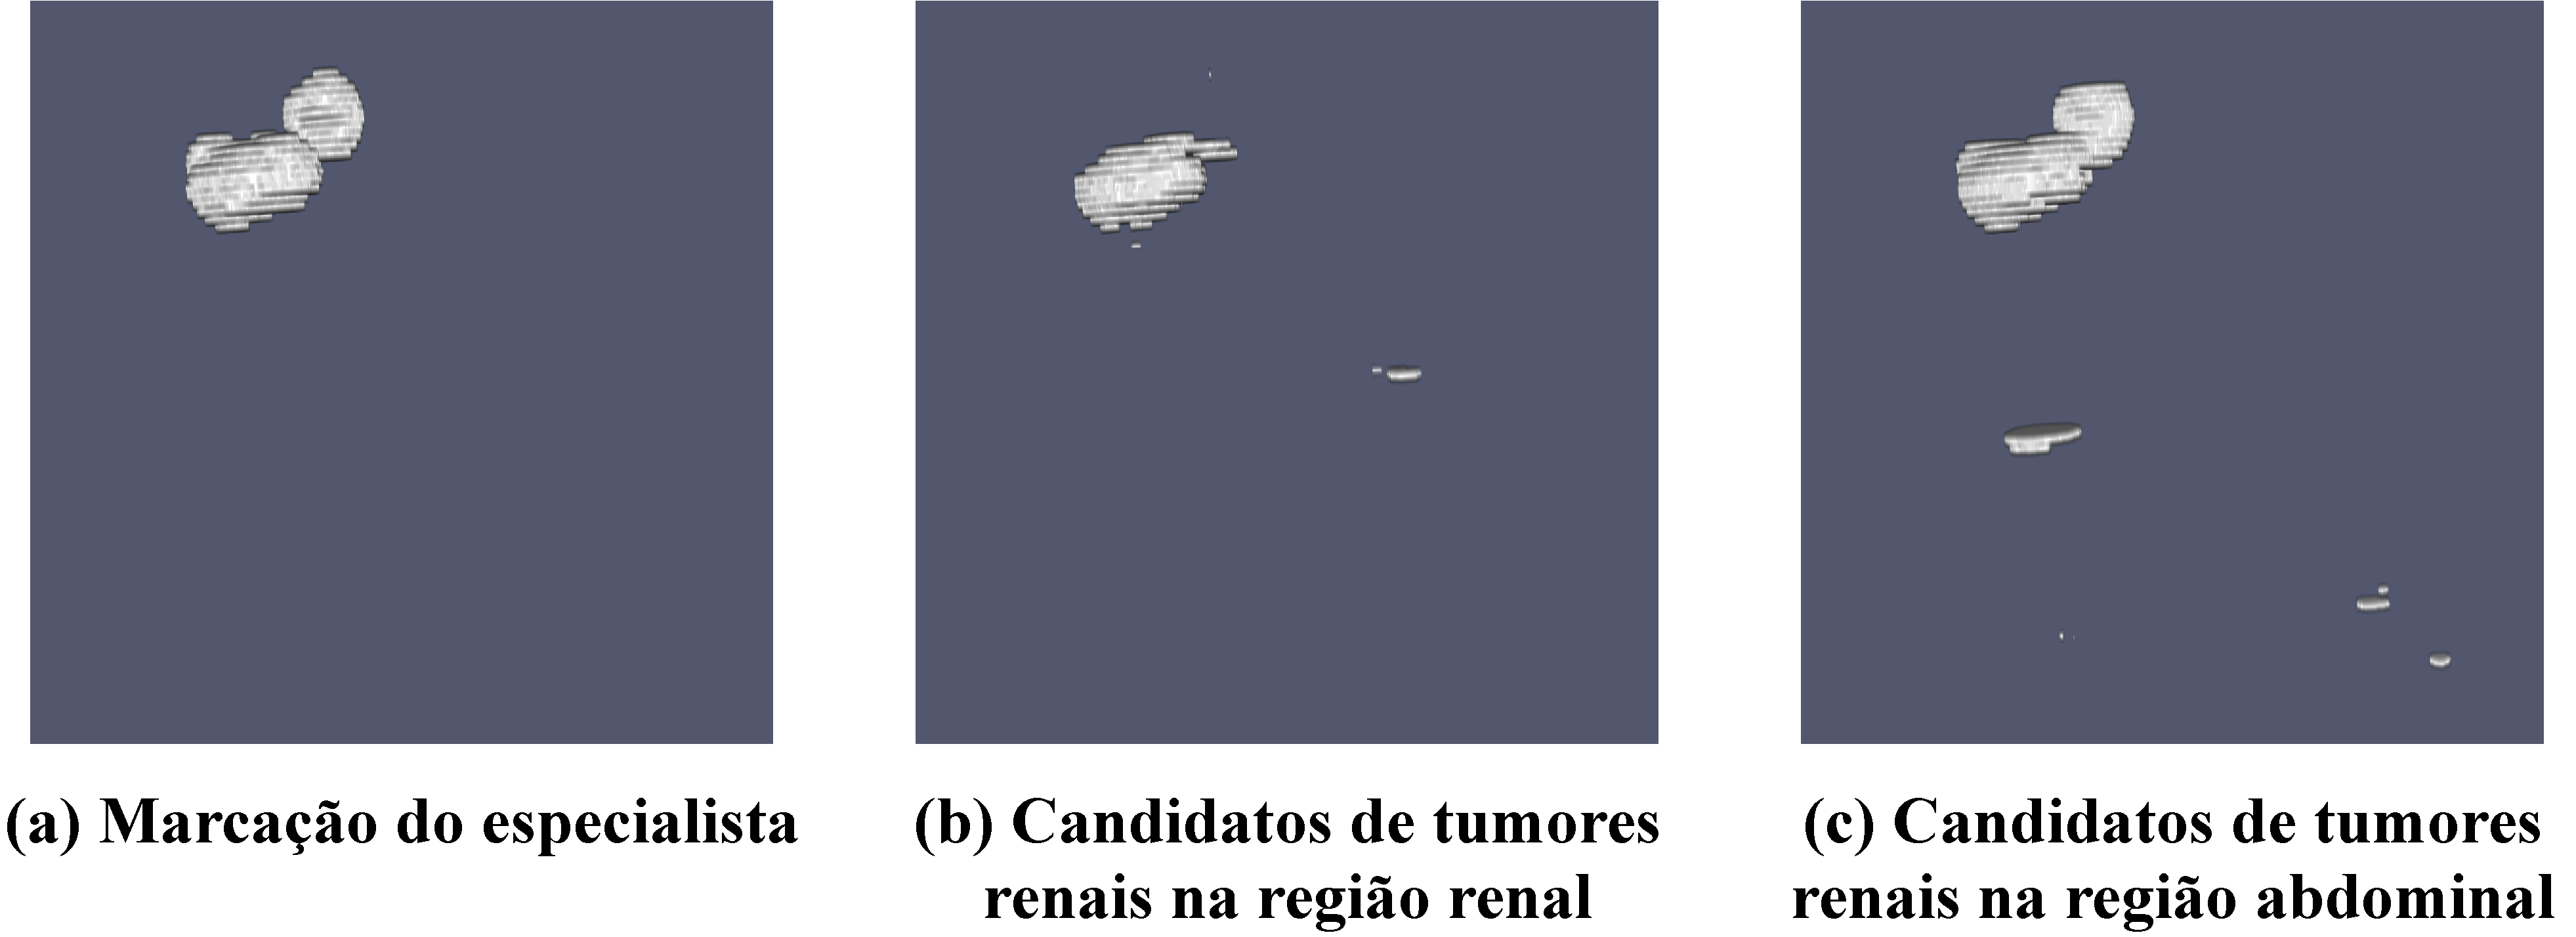
\includegraphics[width=0.9\textwidth]{figuras/candidatos-de-tumores-renais.pdf}
    \legend{Fonte: Elaborado pela autora.}
    \label{fig:candidatos-de-tumores-renais}
\end{figure}

\section{Reconstrução dos Tumores Renais}
\label{sec:metodo-reconstrucao-dos-tumores-renais}

%Em bons cenários, em que os pacientes têm tumores renais bem definidos, apenas a segmentação dos tumores é suficiente para alcançar bons resultados. Porém, em casos difíceis como surgimento de cistos, texturas homogêneas e tumores em estágios avançados (Figura~\ref{fig:casos-dificeis}), o modelo acaba não segmentando bem os tumores renais. Isso se deve ao fato de que o modelo usa informações de textura para realizar a segmentação e, portanto, a diferença de contraste em uma mesma região dos tumores é um fator importante. A Figura xxx ilustra um caso em que a segmentação inicial é comprometida pela situação acima mencionada.

Em bons cenários, onde a segmentação inicial dos rins foi capaz de obter grande parte da região renal, e em que os pacientes apresentam tumores bem definidos, apenas o primeiro estágio é suficiente para alcançar bons resultados. Porém, em casos difíceis como surgimento de cistos, texturas homogêneas, tumores em estágios avançados (Figura~\ref{fig:casos-dificeis}) e perda de regiões renais na segmentação inicial dos rins, o modelo acaba não segmentando bem os tumores.

\begin{figure}[!ht]
    \centering
    \caption{Exemplos de casos difíceis. Rins marcados em azul e tumores renais em vermelho.}
    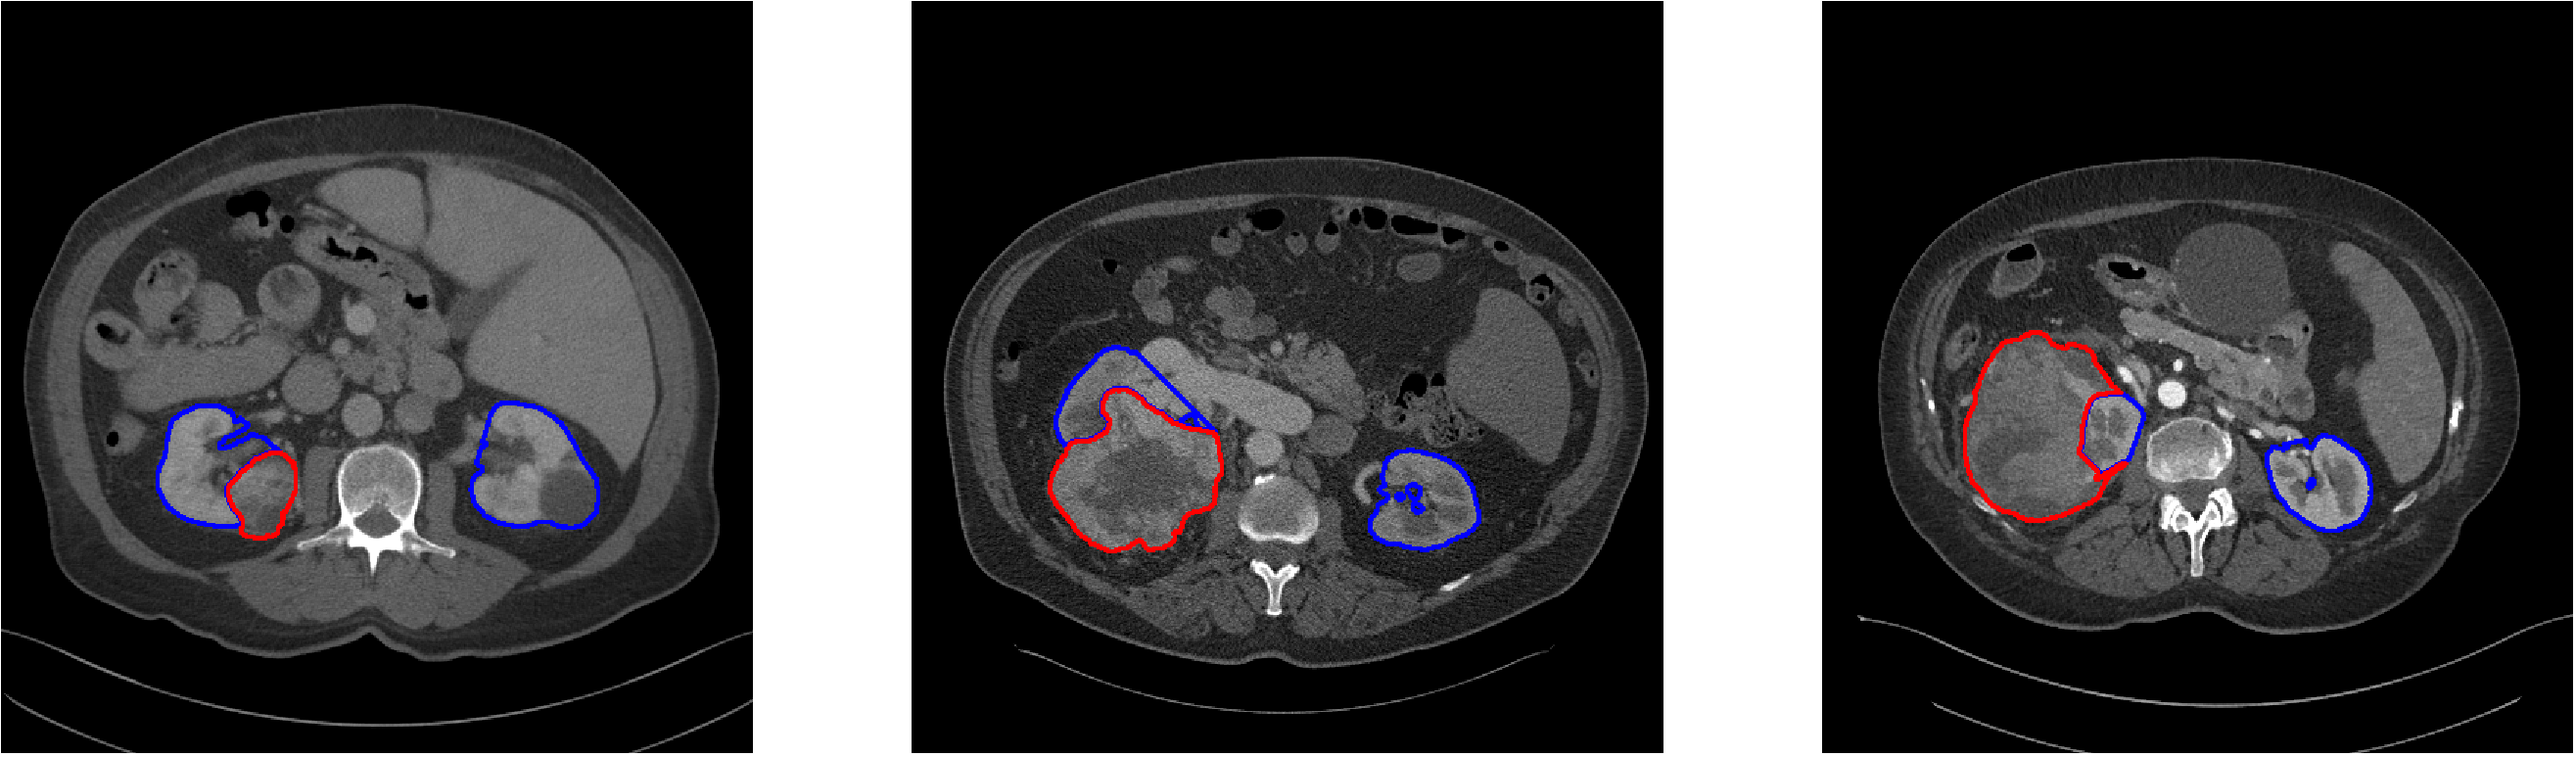
\includegraphics[width=1\textwidth]{figuras/casos-dificeis.pdf}
    \legend{Fonte: Elaborado pela autora.}
    \label{fig:casos-dificeis}
\end{figure}

%A fim de solucionar esses casos particulares e, portanto, desenvolver um modelo de segmentação mais robusto, um segundo modelo de aprendizado profundo é treinado para realizar uma reconstrução dos tumores renais. Esta etapa é dividida em duas subetapas: segmentação dos tumores renais na região de interesse, com ResUNet; e a união da primeira subetapa supracitada com o resultado da segmentação inicial dos tumores renais.

%Com as segmentações adquiridas, o resultado da etapa de reconstrução é obtida pela união da segmentação inicial dos tumores renais e reconstrução dos tumores renais. Para isso, foi realizada uma operação binária (OU) nas duas máscaras de segmentação. A Figura~\ref{fig:reconstrucao-final} mostra um exemplo desse processo.

Dessa forma, o segundo estágio é um fator importante para segmentar regiões que não puderam ser segmentadas no primeiro estágio. No entanto, afim de desenvolver um modelo mais robusto de segmentação de candidatos a tumores, foi realizada uma reconstrução de tumores renais. Esta etapa faz a união entre o primeiro e o segundo estágio usando a operação binária “OU” nas duas máscaras de segmentação. Isso leva a uma segmentação mais precisa da região tumoral, pois partes que não foram segmentadas no primeiro estágio serão segmentadas no segundo estágio, e posteriormente unidas nesta etapa. A Figura~\ref{fig:reconstrucao} mostra um exemplo desse processo.

\begin{figure}[!ht]
    \centering
    \caption{Etapas da reconstrução de tumores renais.}
    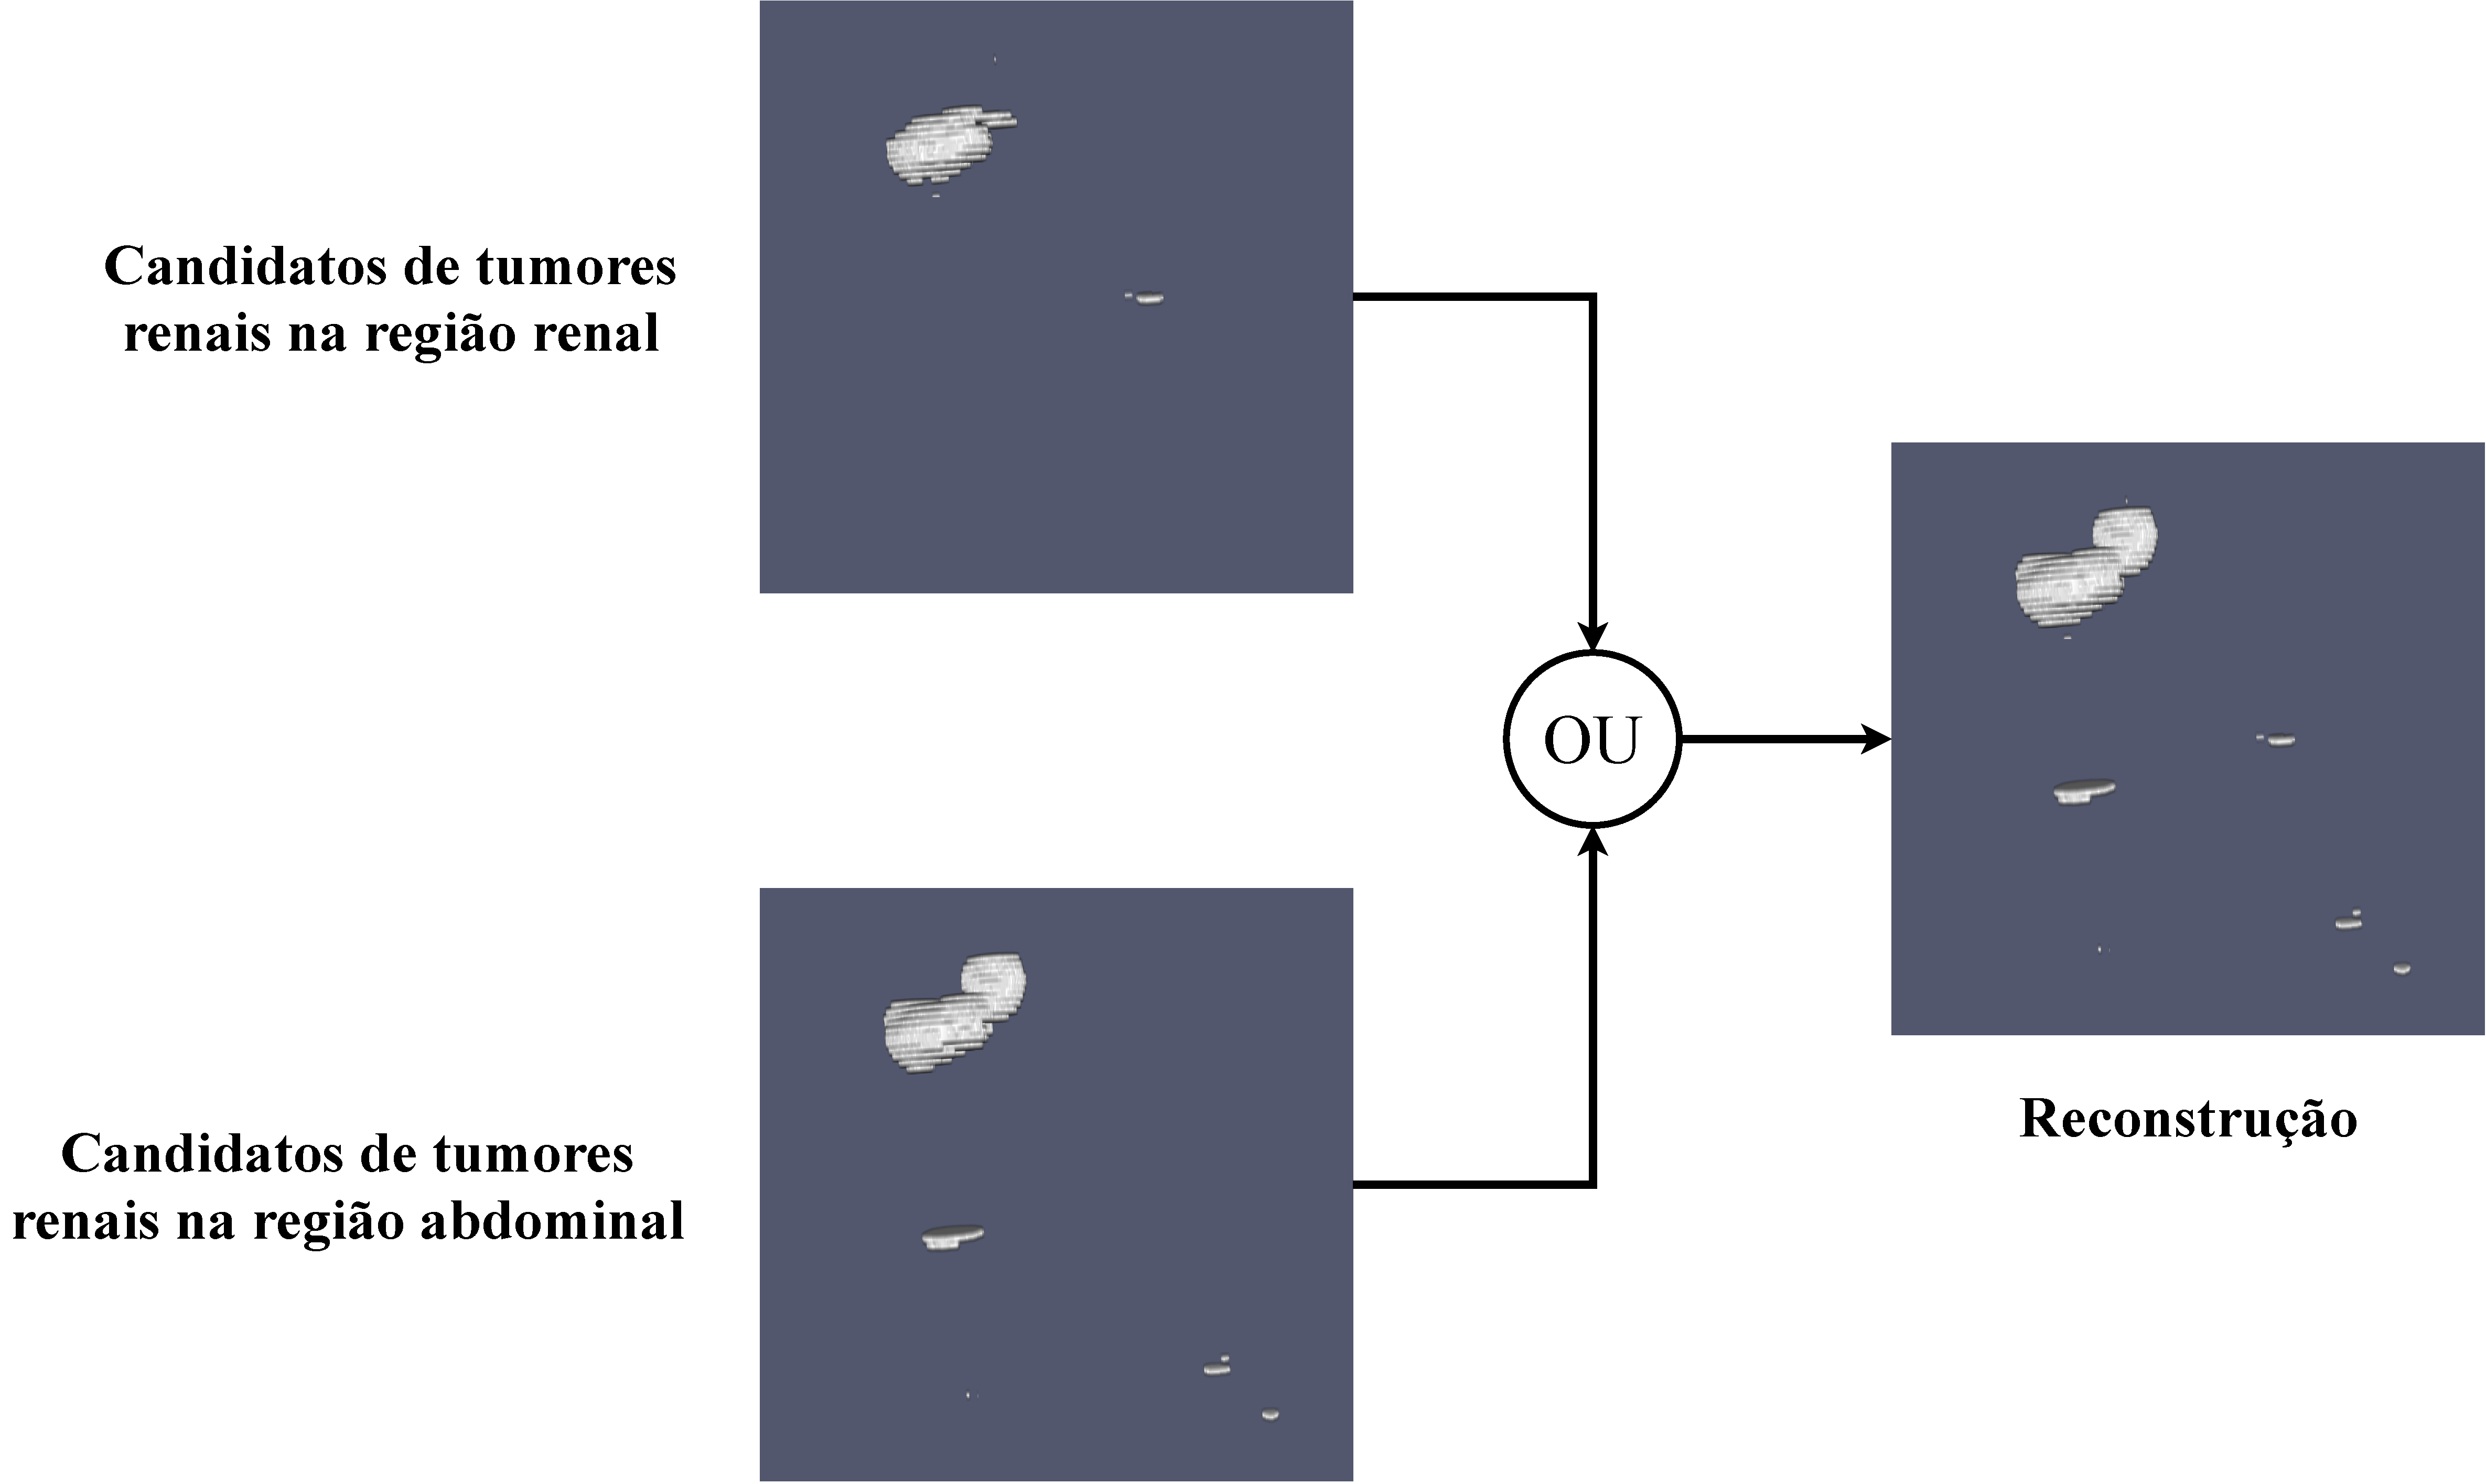
\includegraphics[width=0.9\textwidth]{figuras/reconstrucao.pdf}
    \legend{Fonte: Elaborado pela autora.}
    \label{fig:reconstrucao}
\end{figure}

%O principal benefício da reconstrução é que esta etapa é capaz de recuperar uma porção considerável das regiões tumorais nas quais a diferença de textura o afetou, além de obter uma melhor definição dos contornos tumorais. No entanto, também pode segmentar várias regiões que não são tumores renais. Porém, na etapa final de segmentação, essas regiões segmentadas extras são removidas usando o pós-processamento.

O principal benefício da reconstrução dos tumores renais é que esta etapa é capaz de unir porções consideráveis das regiões tumorais, o que resultou em uma melhor definição dos contornos e regiões tumorais. No entanto, também pode segmentar várias regiões que não são tumores. Porém, na etapa final de segmentação, essas regiões segmentadas extras são removidas usando o pós-processamento.

\section{Redução de Falsos Positivos}
\label{sec:metodo-reducao-falsos-positivos}

Nesta etapa são obtidos os resultados finais das segmentações dos rins e tumores. Para isso, o resultado da etapa de reconstrução dos tumores renais é fundamental para se obter o resultado final dos rins e tumores. Mais detalhes são fornecidos nas próximas subseções.

\subsection{Redução de Falsos Positivos para os Rins}
\label{sec:metodo-reducao-falsos-positivos-rins}

Para obter a segmentação final dos rins, foi feito inicialmente uma união da segmentação inicial dos rins com o resultado da etapa de reconstrução dos tumores renais, usando a operação binária “OU” (Figura~\ref{fig:uniao-rins-recons}). O objetivo é melhorar os contornos que não foram obtidos na etapa de segmentação inicial dos rins por meio da reconstrução dos tumores renais, uma vez que os tumores renais também fazem parte da região renal.

\begin{figure}[!ht]
    \centering
    \caption{União da segmentação inicial dos rins e reconstrução dos tumores renais.}
    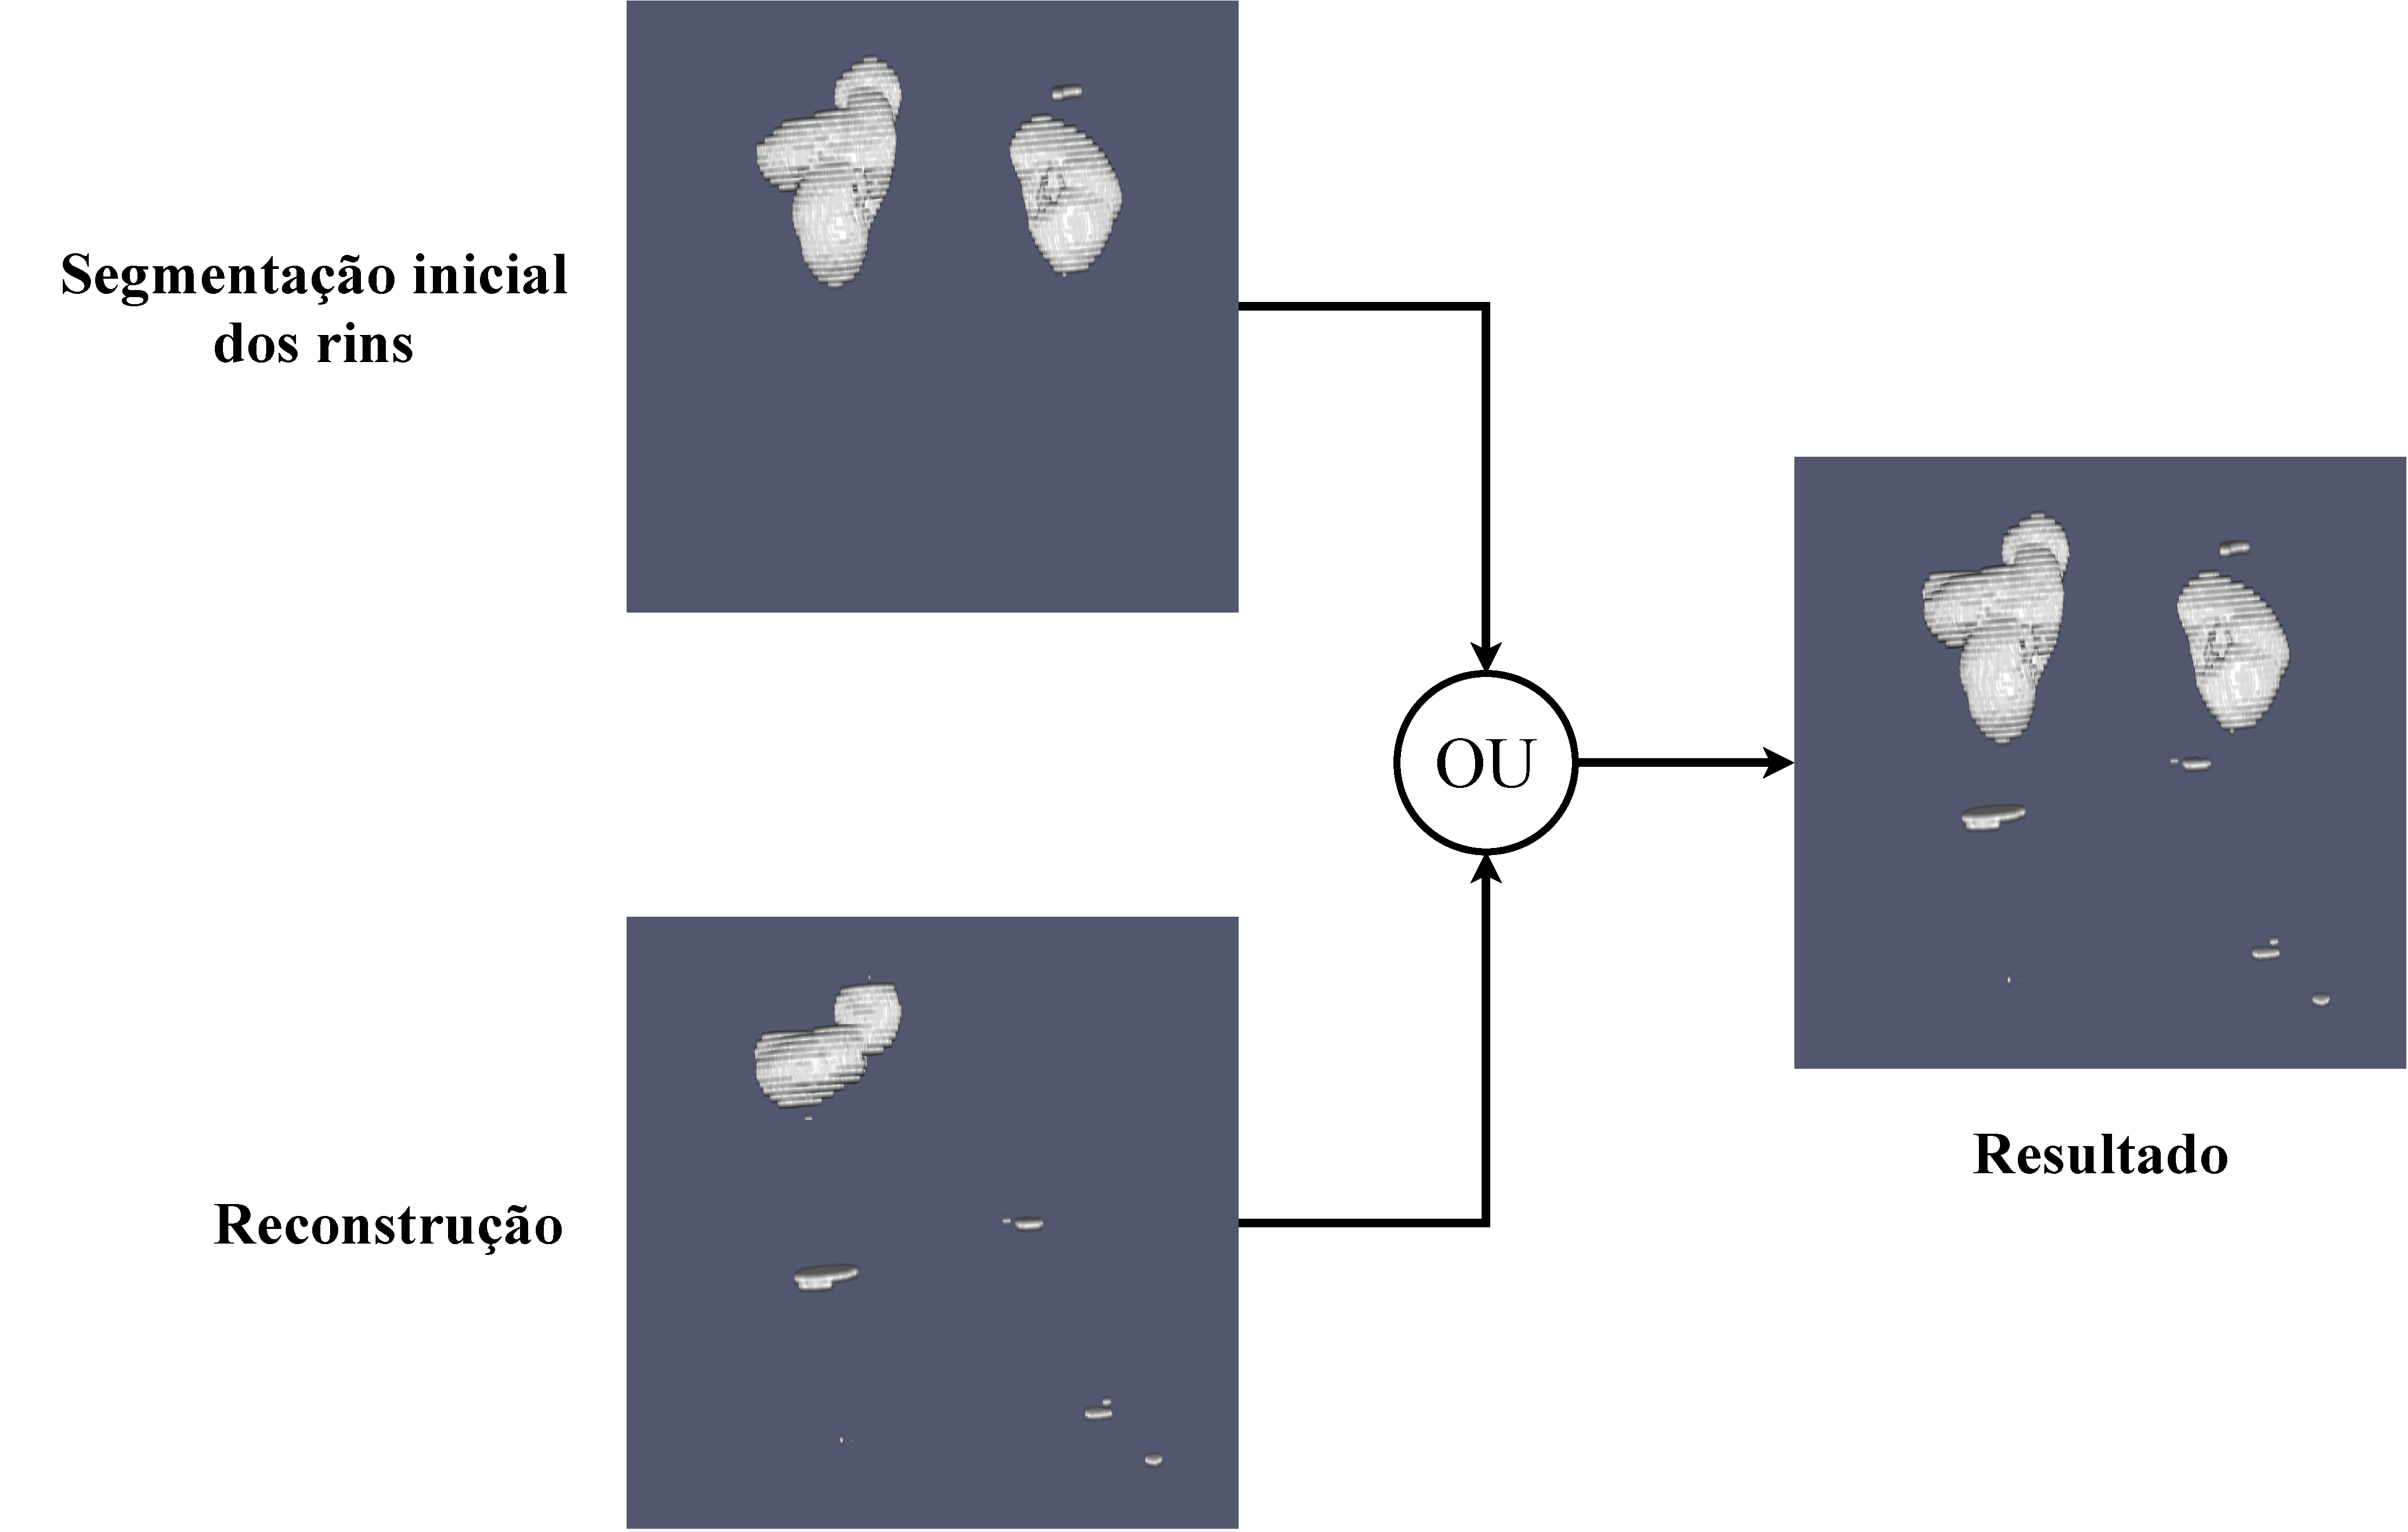
\includegraphics[width=0.9\textwidth]{figuras/uniao-rim-reconstrucao.pdf}
    \legend{Fonte: Elaborado pela autora.}
    \label{fig:uniao-rins-recons}
\end{figure}

No entanto, isso também pode afetar a segmentação inicial dos rins. Portanto, uma etapa de pós-processamento é necessária para remover as regiões que não fazem parte dos rins que foram segmentadas na etapa de união descrita anteriormente. Essa etapa consiste em manter os dois maiores elementos do volume que corresponde aos rins e remover o restante dos fragmentos segmentados (falsos positivos). A Figura~\ref{fig:seg-final-rins}~(a) mostra o resultado em 3D da união descrita anteriormente e a Figura~\ref{fig:seg-final-rins}~(b) a marcação do especialista. Na Figura~\ref{fig:seg-final-rins}~(c) encontra-se o resultado visual após a etapa de pós-processamento. Pode-se observar que alguns fragmentos não renais foram removidos e, consequentemente, a precisão da segmentação dos rins também aumentou.

\begin{figure}[!ht]
    \centering
    \caption{Resultado final da segmentação de rins após pós-processamento.}
    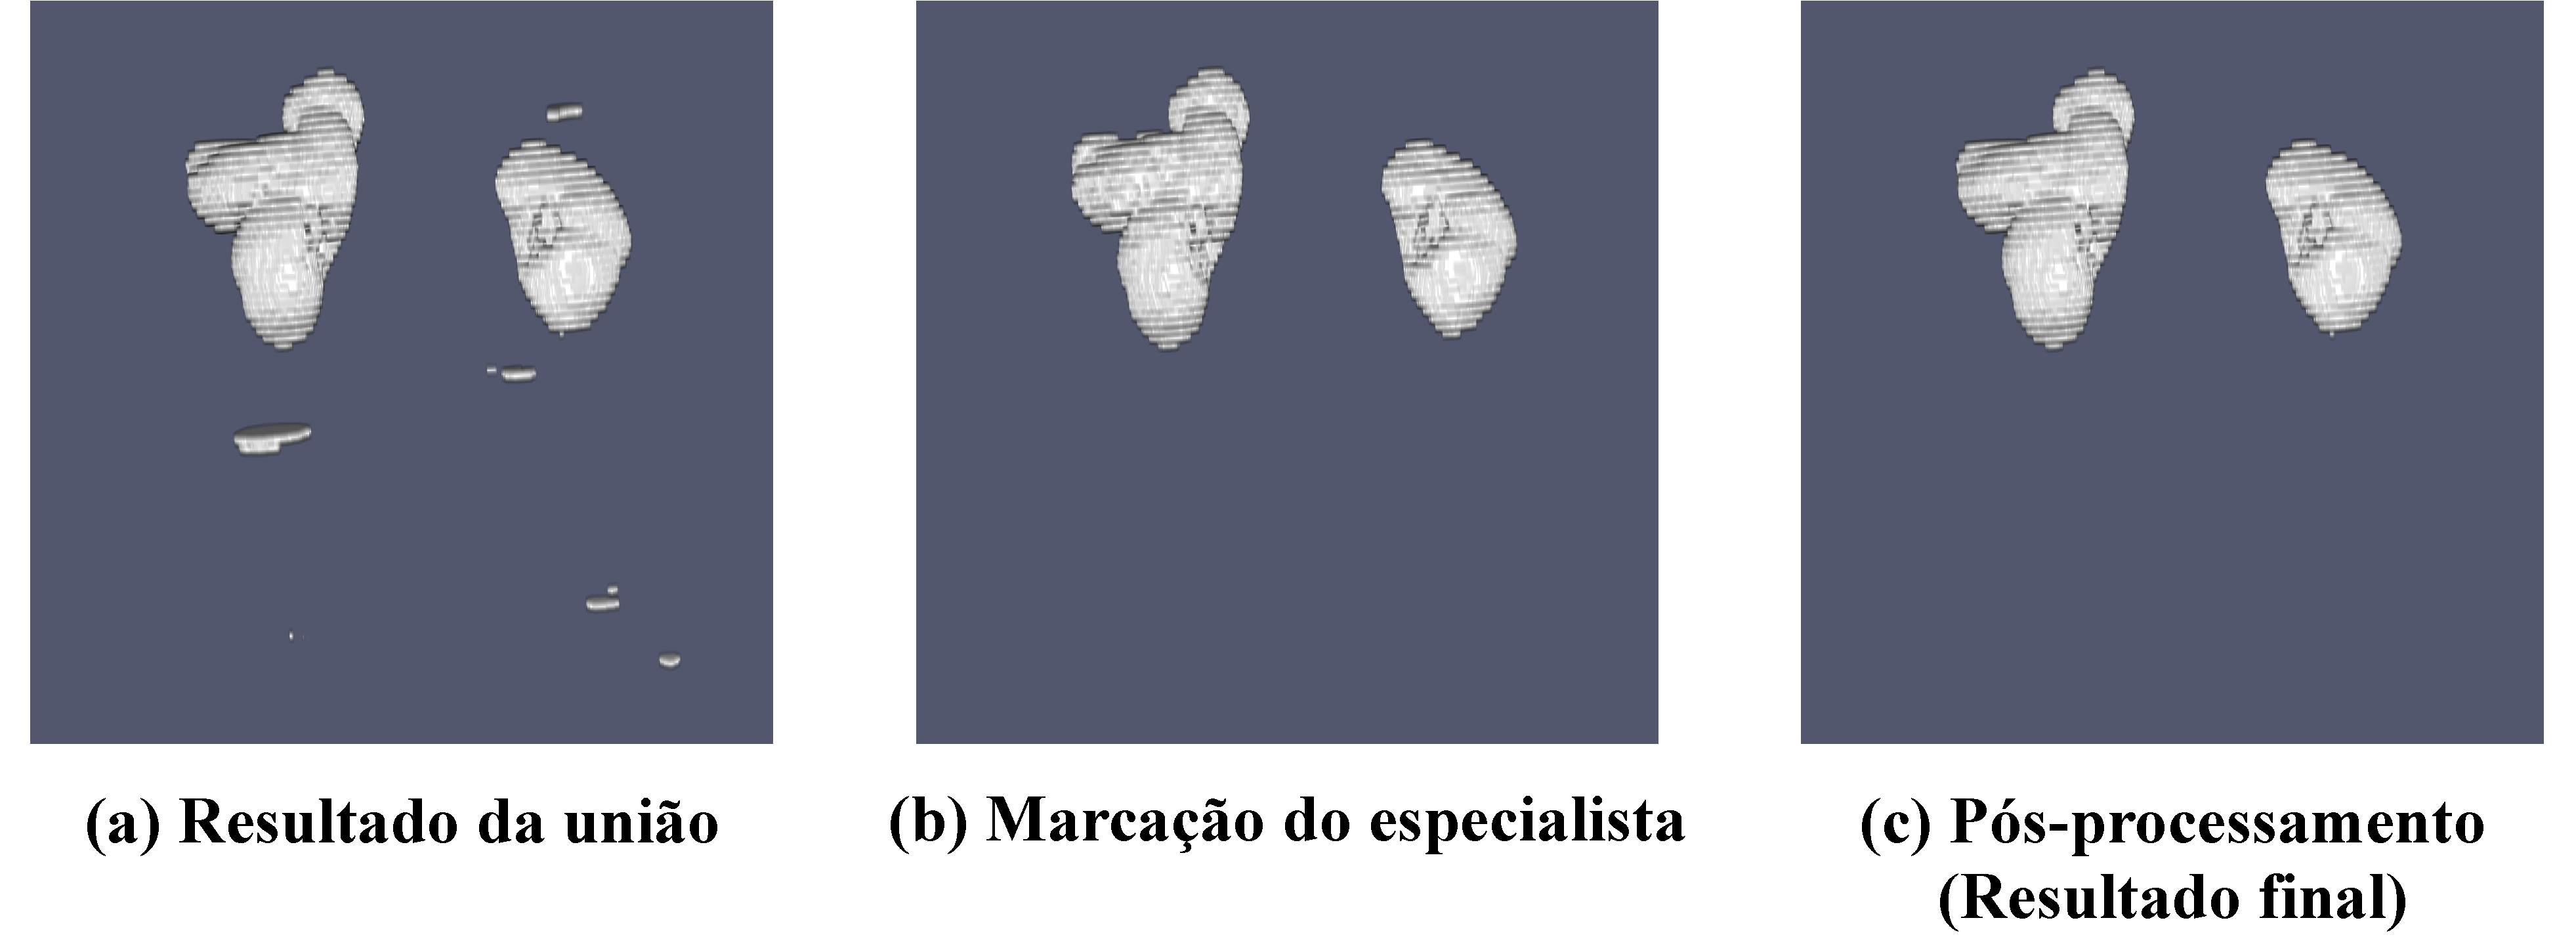
\includegraphics[width=0.9\textwidth]{figuras/rim-final.pdf}
    \legend{Fonte: Elaborado pela autora.}
    \label{fig:seg-final-rins}
\end{figure}

\subsection{Redução de Falsos Positivos para os Tumores Renais}
\label{sec:metodo-reducao-falsos-positivos-tumores-renais}

Nesta subseção são apresentados os procedimentos para obtenção da segmentação final dos tumores renais. Inicialmente, foi aplicada a operação binária “E” para fazer a intersecção da segmentação final dos rins com a etapa de reconstrução dos tumores renais (Figura~\ref{fig:interseccao-rins-recons}). Essa etapa inicial foi feita para extrair apenas a região que contém os tumores, removendo assim parte dos falsos positivos que foram adquiridos na etapa de reconstrução dos tumores renais. Posteriormente, uma etapa de pós-processamento foi aplicada para remover alguns elementos descontínuos que possivelmente eram falsos positivos que permaneceram.

\begin{figure}[!ht]
    \centering
    \caption{Intersecção da segmentação final dos rins e reconstrução dos tumores renais.}
    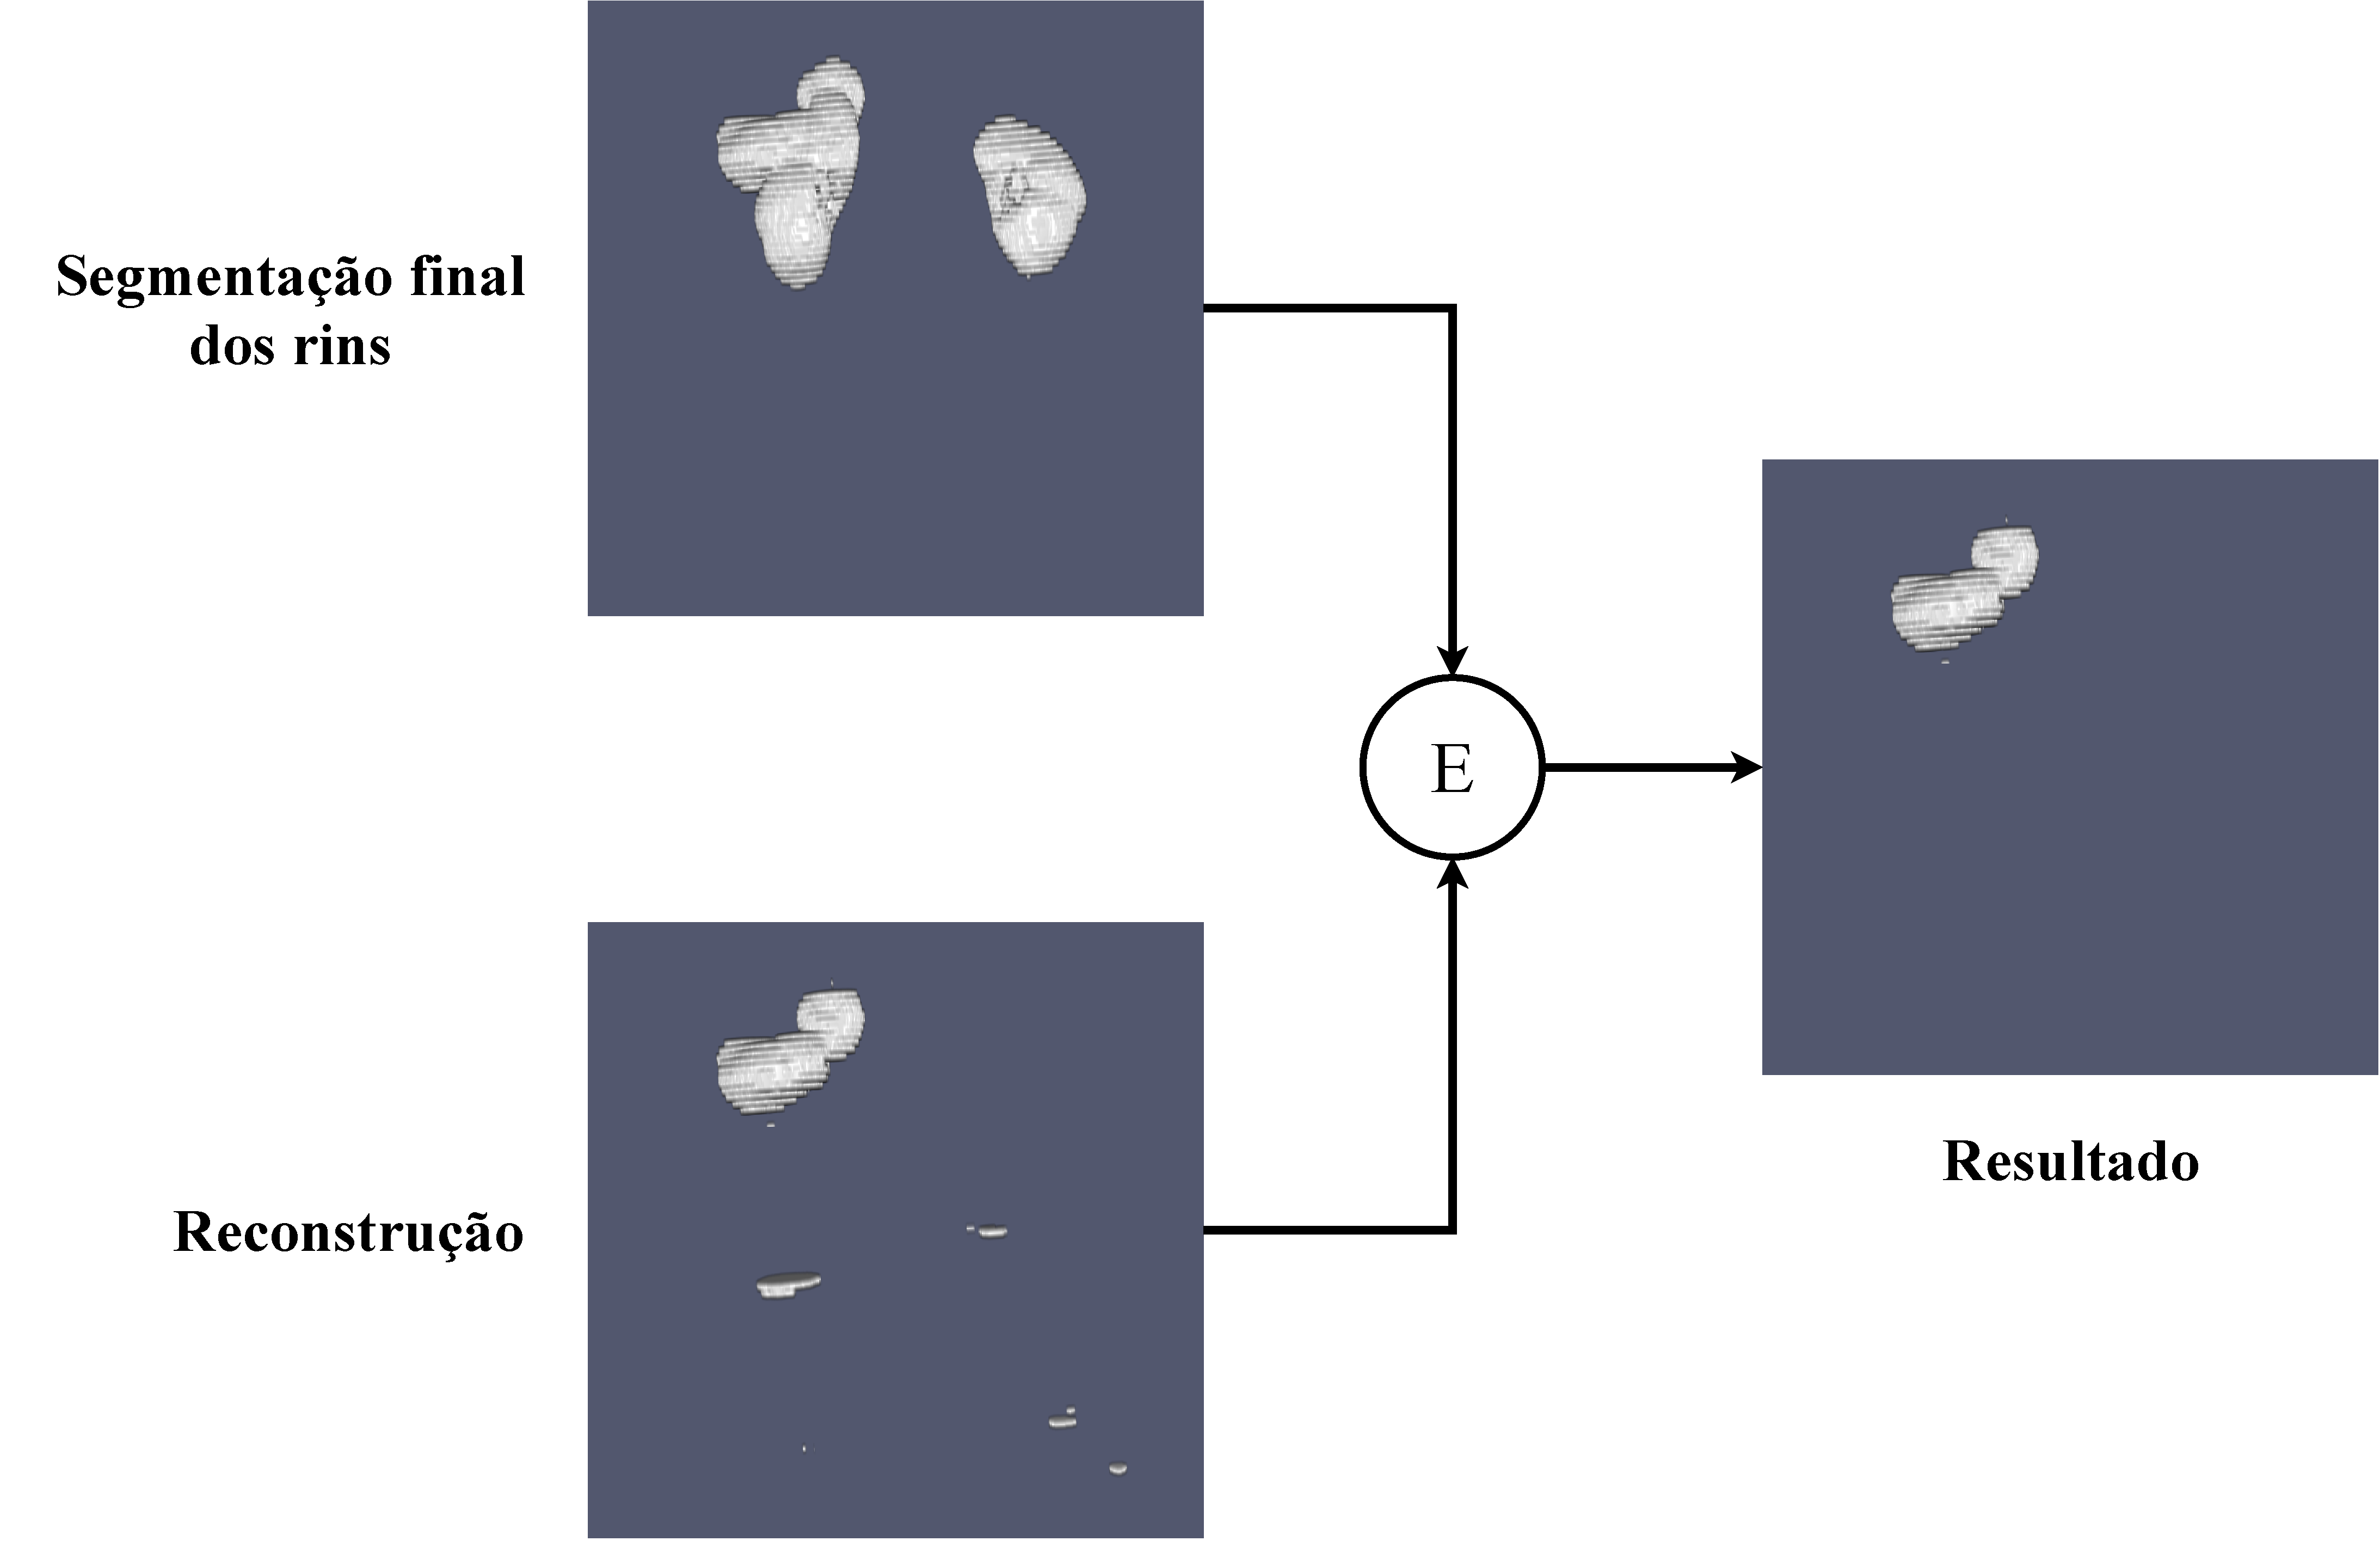
\includegraphics[width=0.9\textwidth]{figuras/interseccao-rim-reconstrucao.pdf}
    \legend{Fonte: Elaborado pela autora.}
    \label{fig:interseccao-rins-recons}
\end{figure}

Os tumores renais são estruturas contínuas que aparecem em várias fatias de um volume de TC~\cite{urology_health,urology_care}. Analisando as informações contextuais vizinhas, o modelo DeepLabv3+ 2.5D resultou na segmentação da fatia central. Portanto, é fundamental verificar se os elementos segmentados pertencem à mesma região. Assim, a etapa de pós-processamento desenvolvida remove as estruturas segmentadas sem informações contextuais suficientes para representar os tumores renais, ou seja, elementos que apresentavam menos de três fatias contínuas.

A Figura~\ref{fig:seg-final-tumores} ilustra a etapa de pós-processamento aplicada. Na Figura~\ref{fig:seg-final-tumores} (a), tem-se o resultado em 3D da interseção descrita acima e a Figura~\ref{fig:seg-final-tumores} (b) mostra a máscara do especialista. Por fim, a Figura~\ref{fig:seg-final-tumores} (c) apresenta o resultado visual após a remoção de elementos descontínuos. É possível verificar que alguns falsos positivos restantes semelhantes aos tumores foram removidos. Assim, a etapa de pós-processamento foi capaz de melhorar a segmentação dos tumores.

\begin{figure}[!ht]
    \centering
    \caption{Resultado final da segmentação de tumores renais após a aplicação do pós-processamento.}
    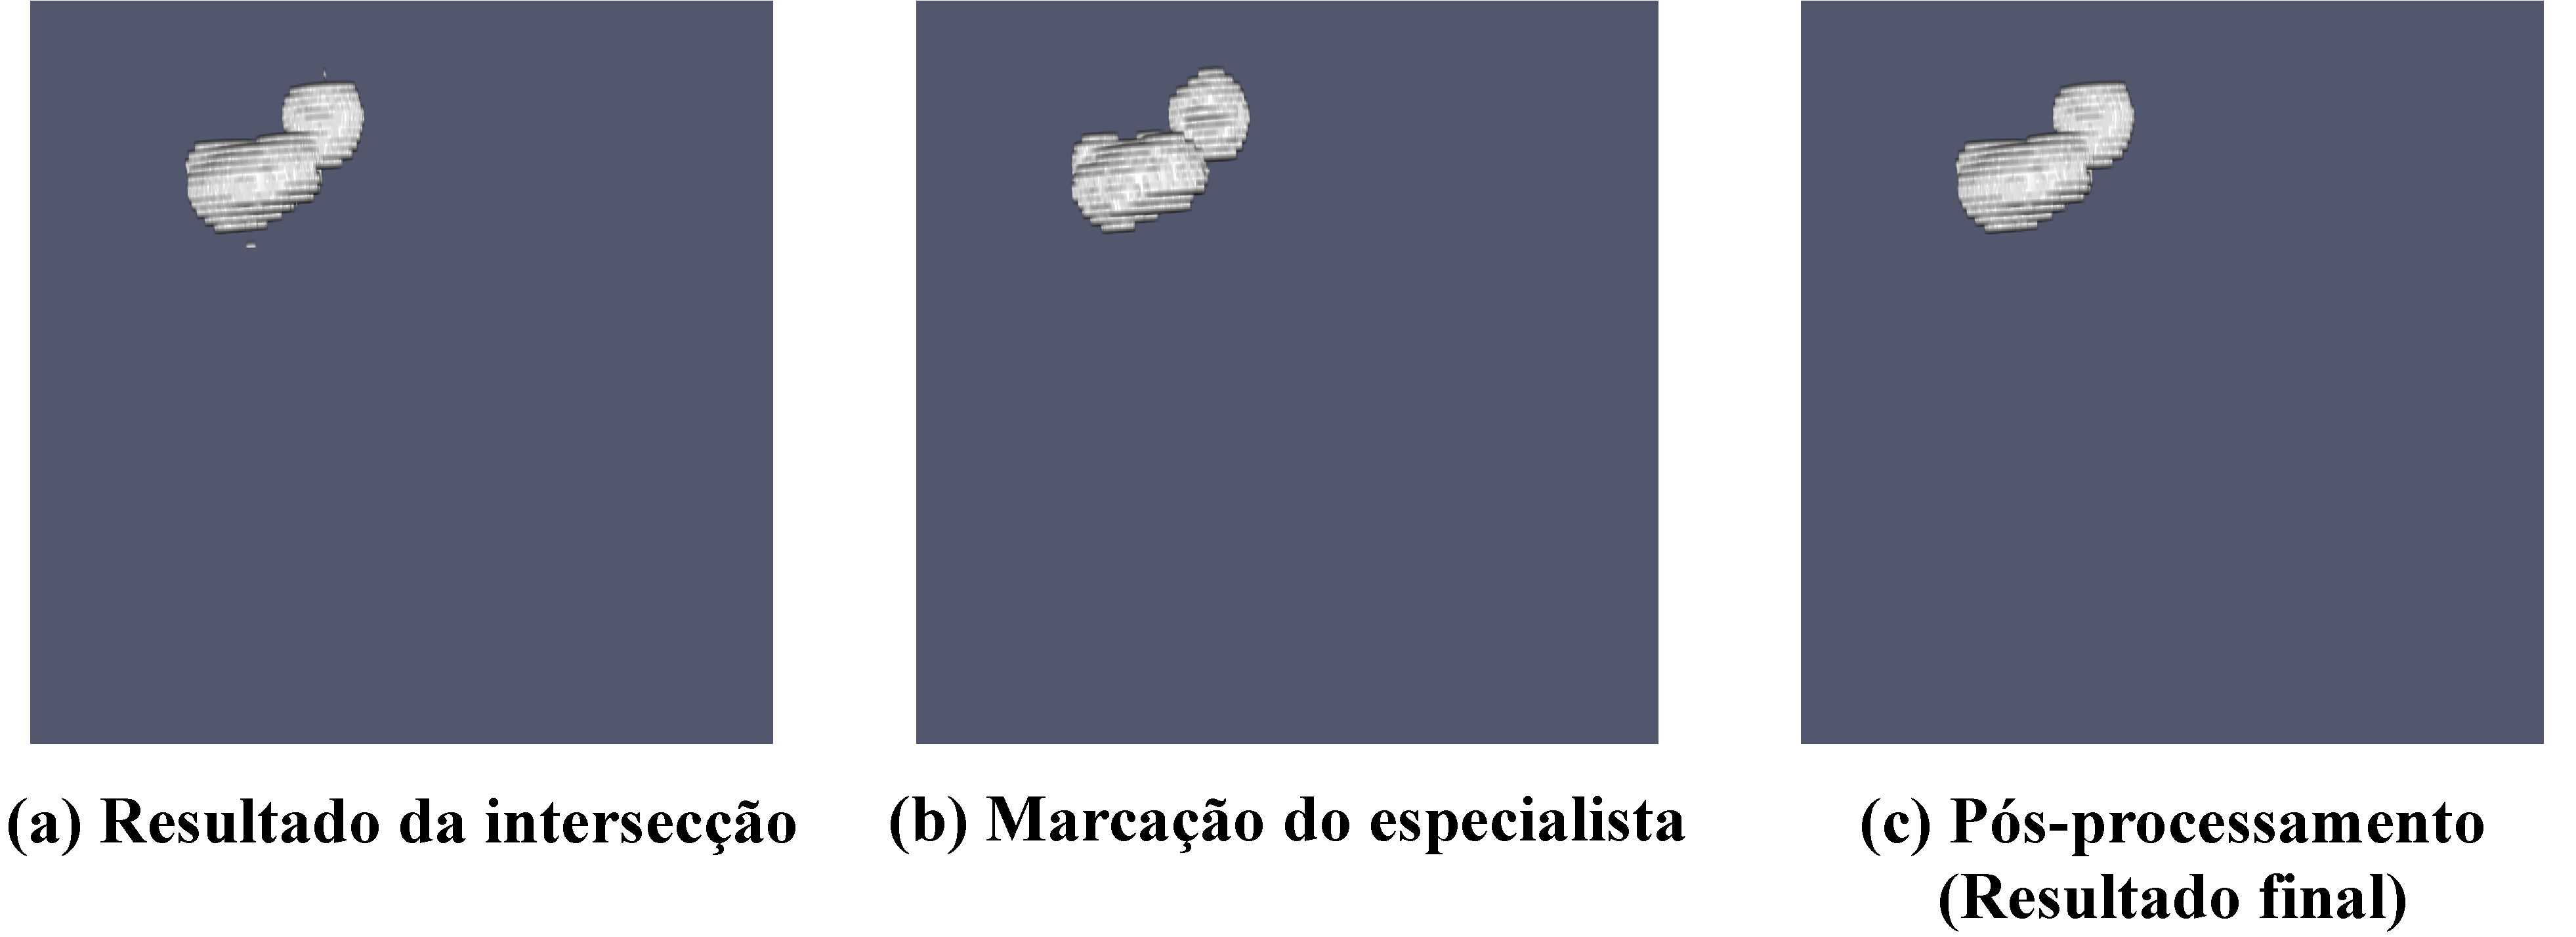
\includegraphics[width=0.9\textwidth]{figuras/tumor-final.pdf}
    \legend{Fonte: Elaborado pela autora.}
    \label{fig:seg-final-tumores}
\end{figure}

\section{Considerações Finais}
\label{consideracoes-finais-metodo}

Este capítulo apresentou e descreveu em detalhes o método proposto para segmentação de rins e tumores em imagens de TC. Foram detalhadas cada uma das etapas que compõem o método, e apresentadas as adaptações empregadas para a segmentação de rins e tumores nesta tese. Entre as principais contribuições estão: a distribuição proporcional da base de imagens; balanceamento de fatias do alvo de segmentação; segmentação de rins e candidatos a tumores renais na região abdominal usando o modelo ResUNet 2.5D; combinação do modelo DeepLabv3+ com o codificador DPN-131 para segmentação de candidatos a tumores renais na região renal; reconstrução dos tumores renais usando operações binárias; e técnicas de processamento de imagens para redução de falsos positivos com base em informações contextuais.

%No próximo capítulo, serão apresentados os resultados com a aplicação do método proposto. Será feita uma discussão acerca dos resultados obtidos, e também uma comparação com os trabalhos descritos na literatura, visando contextualizar a relevância da pesquisa desenvolvida neste trabalho.

No próximo capítulo, serão apresentados os resultados obtidos em cada uma das etapas do método proposto. Além disso, são apresentadas a base de imagens aplicada, a configuração experimental das redes usadas e alguns experimentos para validar as etapas do método proposto.

% marcador natural; estimação de pose; 
\chapter{Resultados}
\label{cap:resultados}
\phantom{0}

%Este capítulo apresenta e discute os resultados experimentais de cada etapa do método proposto. O procedimento de avaliação dos resultados foi o seguinte: 1) preparação da base de imagens e configuração experimental; 2) resultados iniciais da segmentação de rins e tumores renais; 3) reconstrução dos tumores renais; e 4) resultados finais da segmentação de rins e tumores renais.

Este capítulo apresenta os resultados experimentais de cada etapa do método proposto. Primeiramente, é apresentada a base de imagens que foi usada. Em seguida, é mostrada a avaliação dos resultados, com os seguintes procedimentos: 1) configuração experimental; 2) resultados gerais do método proposto; 3) resultados iniciais da segmentação de rins; 4) resultados iniciais de candidatos a tumores renais; 5) reconstrução dos tumores renais; e 6) resultados finais da segmentação de rins. 

\section{Base de Imagens}
\label{sec:conjunto-dados}

Neste trabalho, a base de imagens usada para realizar os experimentos foi de um desafio denominado KiTS19. Este desafio teve como objetivo acelerar a pesquisa e desenvolver novos recursos nefrométricos para auxiliar no prognóstico do tumor renal e no planejamento do tratamento; e também a criação de métodos confiáveis de segmentação semântica para rim e tumor renal~\cite{1904.00445}.

A base de imagens KiTS19 consiste em TCs de pacientes que foram submetidos a nefrectomia parcial ou radical para um ou mais tumores renais. Os exames foram coletados pelo Centro Médico da Universidade de Minnesota (\textit{University of Minnesota Medical Center}) entre 2010 e 2018. De acordo com o desafio, a base de imagens contém 300 TCs, divididos em 210 TCs para treinamento e validação e os 90 restantes para avaliar o desempenho do modelo. Para o conjunto de treinamento e validação, o desafio disponibilizou máscaras de segmentação semântica (anotações) e foram esses conjuntos de imagens que foram usados para realizar os experimentos desta tese. Essas anotações foram fornecidas por estudantes de medicina que realizaram segmentações manuais sob a supervisão dos radiologistas e patologistas cirúrgicos (Drs. Christopher Weight e Niranjan Sathianathen). Isso ajudou na localização precisa dos tumores para evitar classificação incorreta como cistos que também podem estar presentes~\cite{1904.00445}.

Todos os pacientes foram tratados por urologistas em um único centro de atendimento e mais da metade dos exames foram adquiridos em mais de 50 instituições de referência. Para cada instituição, uma variedade de protocolos de aquisição é aplicada. Isso torna a base de imagens KiTS19 diversa em termos de dimensões de \textit{voxel}, tempo de contraste, assinatura de tabela e campo de visão do scanner. Além disso, ajuda a minimizar algumas preocupações sobre a validade externa de um coorte retrospectivo\footnote{O pesquisador colhe informação pregressa dos fatores de exposição e acompanha por um período de tempo os indivíduos~\cite{CAMARGO2019}.} de uma única instituição, como o KiTS19~\cite{HELLER2021101821}.

Cada volume de TC (imagens e máscaras) foi fornecido no formato NIFTI~\cite{NIFTI}. Todos os volumes têm resolução $512\times512$ em escala de cinza, e o número de fatias varia de 29 a 1059. O método proposto tem como objetivo segmentar os rins e também os tumores renais entre os cistos presentes, o que é um desafio devido às semelhanças. A Figura~\ref{fig:ExImagemEMascara} ilustra um exemplo de fatia de um volume, que contém as marcações: rins (azul) e tumores (vermelho).

\begin{figure}[ht!]
    \centering
    \caption{Informações da base de imagens: fatia com marcações de rins (azul) e tumores (vermelho).}
    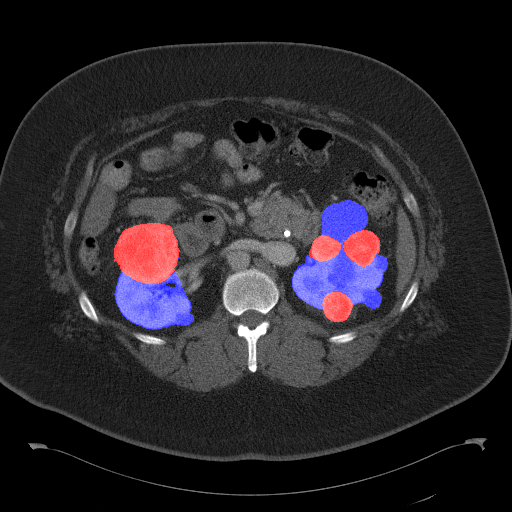
\includegraphics[width=0.55\textwidth]{figuras/exemplo-dataset.png}
    \legend{Fonte: Elaborado pela autora.}
    \label{fig:ExImagemEMascara}
\end{figure}

\subsection{Distribuição Proporcional da Base de Imagens}
\label{sec:res-distribuicao-proporcional-dataset}

Esta seção apresenta o resultado da aplicação do método para distribuição proporcional da base de imagens. Para realizar os experimentos, foi usada a base de imagens KiTS19, na qual o conjunto de teste (31 TCs) foi inicialmente selecionado aleatoriamente entre os 210 TCs disponíveis. Os demais exames de TC foram usados como entrada para o método, seguindo as três etapas principais (Seção~\ref{sec:distribuicao-proporcional-dataset}): (1) reamostrar os exames; (2) extrair \textit{deep features}; e (3) agrupar.

É importante mencionar que antes de reamostrar os exames, a quantidade de fatias de tumores renais em cada exame variou de 3 a 256. A primeira etapa, foi realizada a técnica de reamostragem dos exames de TC. Na qual, obteve-se o valor médio de fatias de exames de TC por meio da operação média, que consistiu em calcular a quantidade total de fatias de tumores (4.927) contidos no conjunto de treino e validação, e dividir pela quantidade de exames totais (179). Como resultado, o valor médio foi de 27 fatias. Por fim, foi aplicada a técnica de reamostragem e todos os exames passaram a ter 27 fatias.

Na segunda etapa, são extraídas as \textit{deep features} dos exames reamostrados. A Tabela~\ref{tab:numero-caracteristicas} mostra o número de características extraídas dos exames para cada modelo descrito na Seção~\ref{sec:distribuicao-proporcional-dataset}.

\begin{table}[!ht]
\caption{Total de características extraídas em cada modelo de CNN.}
\label{tab:numero-caracteristicas}
\centering
\begin{tabular}{c|c|c}
\hline
Modelo     & N° de características por fatia & Total (27 fatias) \\ \hline
ResNet-18  & 512                             & 13.824             \\ \hline
ResNet-34  & 512                             & 13.824             \\ \hline
ResNet-101 & 2.048                            & 55.296             \\ \hline
VGG-11     & 1.000                            & 27.000             \\ \hline
VGG-16     & 1.000                            & 27.000             \\ \hline
DPN-131    & 2.688                            & 72.576             \\ \hline
Xception   & 2.048                            & 55.296             \\ \hline
\end{tabular}
\end{table}

Na terceira etapa, as características extraídas por cada modelo são usadas para realizar o agrupamento de dados. A Tabela~\ref{tab:melhores-grupos} apresenta os modelos, o melhor grupo encontrado dentre os K-grupos (2 a 20) e o valor da inércia. Dentre eles, o modelo ResNet-34, que tem o valor seis representando o melhor grupo, foi o escolhido por apresentar a menor inércia (49.158).

\begin{table}[!ht]
\caption{Melhores grupos e suas inércias encontrados para os modelos usando o método do cotovelo.}
\label{tab:melhores-grupos}
\centering
\begin{tabular}{c|c|c}
\hline
Modelo     & N° ótimo de grupos & Inércia       \\ \hline
ResNet-18  & 6                  & 55.260        \\ \hline
\rowcolor[HTML]{C0C0C0} 
ResNet-34  & 6                  & 49.158        \\ \hline
ResNet-101 & 5                  & 83.542        \\ \hline
VGG-11     & 6                  & 248.324.688   \\ \hline
VGG-16     & 8                  & 134.276.912   \\ \hline
DPN-131    & 7                  & 5.828.450.304 \\ \hline
Xception   & 6                  & 2.972.436     \\ \hline
\end{tabular}
\end{table}

A Figura~\ref{fig:distribuicao-proporcional} apresenta o gráfico com o número de exames para cada um dos grupos encontrados. Finalmente, os casos (exames) de cada um dos seis grupos gerados pelo método proposto foram selecionados aleatoriamente e distribuídos proporcionalmente entre os conjuntos de dados de treinamento (148 exames) e validação (31 exames).

\begin{figure}[!ht]
    \centering
    \caption{Grupos de tumores encontrados com a aplicação do método a partir dos conjuntos de treinamento e validação.}
    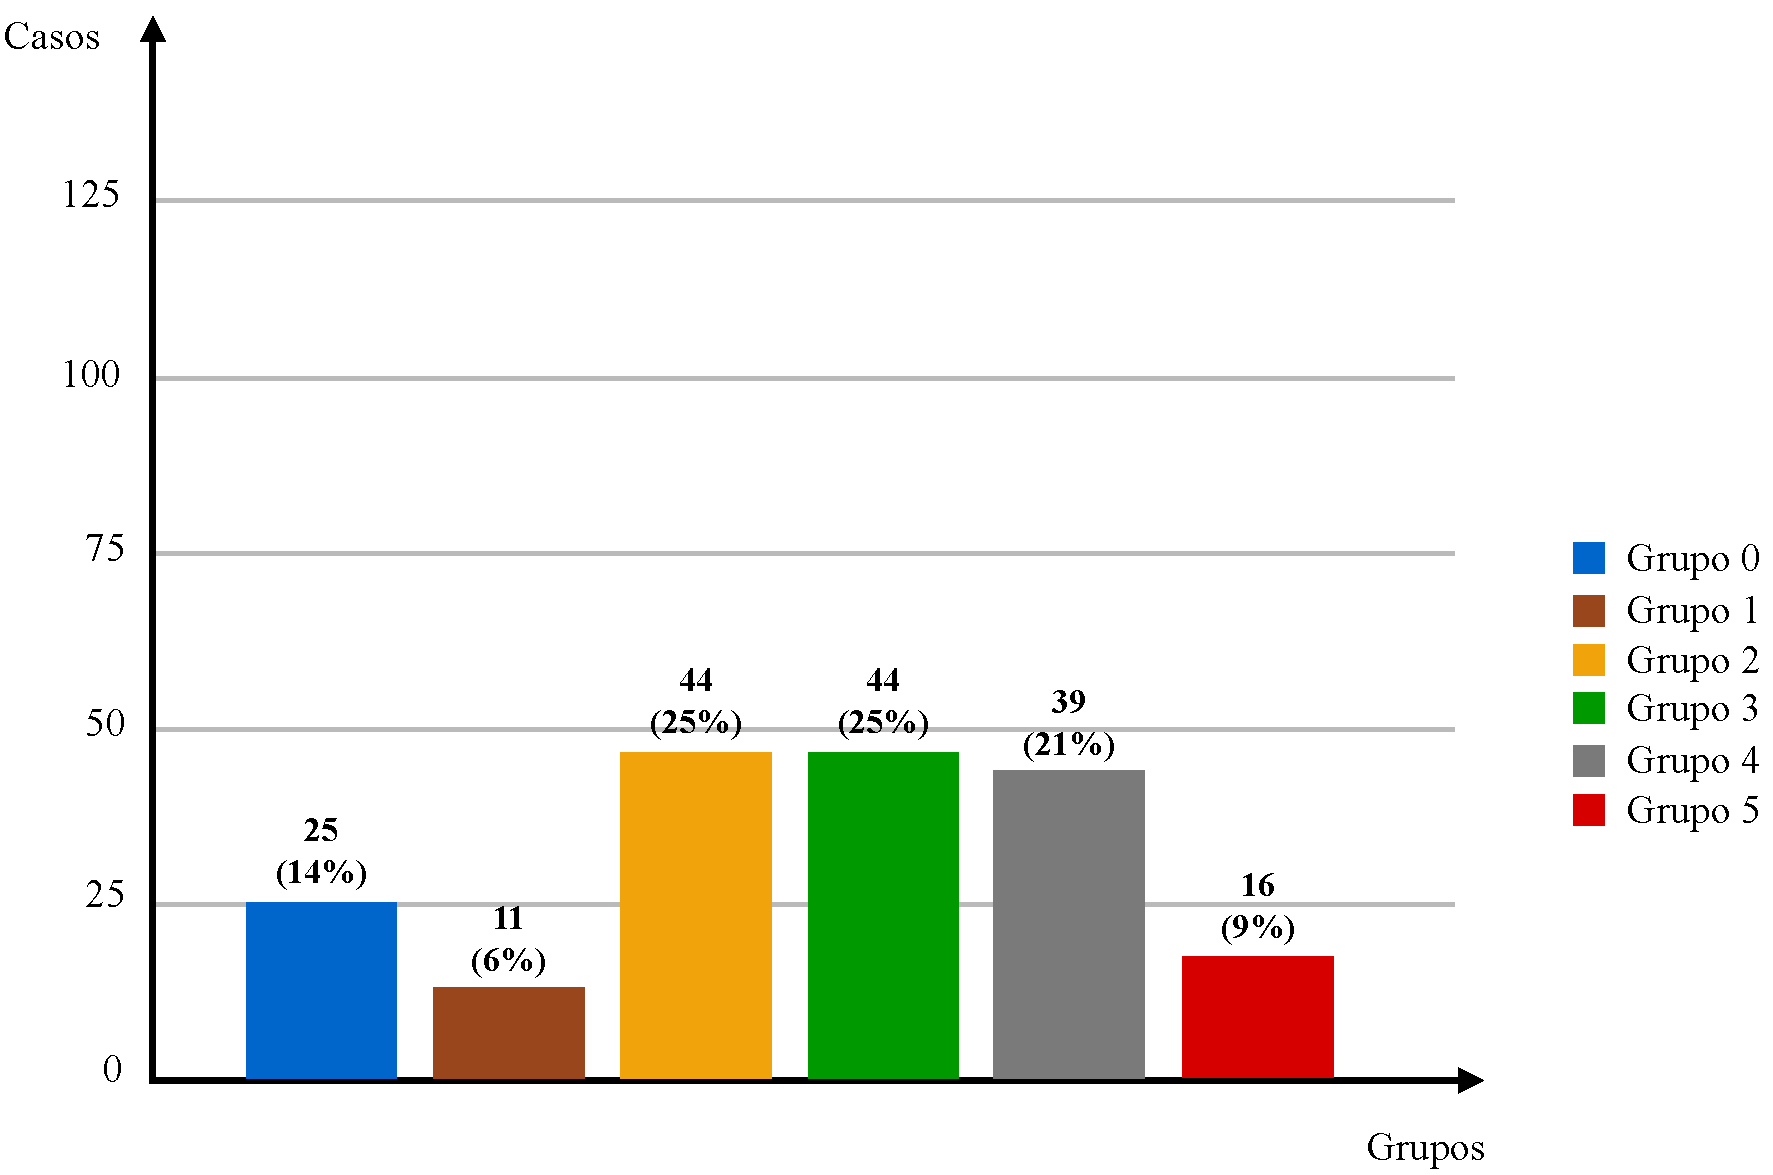
\includegraphics[width=0.75\textwidth]{figuras/distribuicao-proporcional.pdf}
    \legend{Fonte: Elaborado pela autora.}
    \label{fig:distribuicao-proporcional}
\end{figure}

\subsection{Preparação da Base de Imagens}
\label{sec:preparacao-conjunto-dados}

Inicialmente, os volumes de TC foram pré-processados (Seção~\ref{sec:pré-processamento}) antes de serem usados como entrada para a ResUNet 2.5D (Seções~\ref{sec:metodo-segmentacao-dos-rins-ResUNet} e \ref{sec:metodo-candidatos-tumores-renais-regiao-abdominal}) e DeepLabv3+ 2.5D (Seção~\ref{sec:metodo-candidatos-tumores-renais-regiao-renal}). Para fins de teste e validação, foram separados aproximadamente 148 (70\%) volumes de TC para treinamento, 31 (15\%) para validação e 31 (15\%) para teste do conjunto de 210 TCs disponíveis. Inicialmente, o conjunto de teste foi selecionado aleatoriamente (31 casos), e com os casos restantes (179 casos), uma distribuição proporcional foi feita para separar os casos entre os conjuntos de treinamento e validação, conforme descrito na Seção~\ref{sec:res-distribuicao-proporcional-dataset}. Além disso, foi realizado um balanceamento de fatias para cada modelo de aprendizado profundo (Seções~\ref{sec:treinamento-ResUNet}, \ref{sec:treinamento-DeepLabv3+} e \ref{sec:metodo-candidatos-tumores-renais-regiao-abdominal}).

\section{Configuração Experimental}
\label{sec:configuracao-experimental}

O método proposto foi implementado usando a linguagem de programação Python e principalmente a biblioteca de aprendizado profundo Pytorch~\cite{NEURIPS2019_9015}. O computador usado nos experimentos consistia em uma CPU Intel Core i7-7700K 4.20GH, 16 GB de RAM e placa de vídeo Nvidia GeForce GTX 1080-Ti, executado no sistema operacional Windows 10.

O critério de parada nos modelos de treinamento foi usando a técnica early stop~\cite{brownlee2018better}, que consiste em parar o treinamento da rede quando a métrica monitorada (o valor da função de perda nos dados de validação) parasse de melhorar em 15 épocas. Os hiperparâmetros usados nos modelos tinham um tamanho de \textit{batch} igual a 8, função de perda Dice~\cite{dice1945}, otimizador estocástico Adam~\cite{adam2014} com uma taxa de aprendizagem inicial de 0,0001 com decaimento de 10\% se o valor da função de perda nos dados de validação não cair em 7 épocas, beta-1 0,9 e beta-2 0,999 (taxas de decaimento iniciais usadas ao estimar o primeiro e o segundo momentos do gradiente). Após a aplicar o algoritmo de otimização \textit{Tree of Parzen Estimators} (TPE) usando a biblioteca Hyperopt~\cite{bergstra2013making}, este foi o conjunto de hiperparâmetros que produziu os melhores resultados. O tempo de execução total de otimização foi de aproximadamente 4 semanas.

As métricas (Seção~\ref{sec:metricas-de-desempenho}) usadas para avaliar o desempenho do método proposto foram: coeficiente de similaridade Dice (Dice), índice de Jaccard (Jacc), acurácia (Acc), sensibilidade (Sen) e especificidade (Esp). Além disso, foram realizados testes de significância\footnote{Teste de significância é um procedimento estatístico que permite tomar uma decisão entre duas ou mais hipóteses (rejeitar ou não rejeitar), usando os dados observados de um determinado experimento~\cite{statistical1982, zou2003}.} das etapas do método.

\section{Resultados Gerais do Método Proposto}
\label{sec:resultados-metodo-proposto}

Nesta seção, são apresentados os resultados obtidos em cada etapa do método proposto. Para que o método fosse validado, os conjuntos de treino, validação e teste foram distribuídos 5 vezes usando os mesmos procedimentos descritos na Seção~\ref{sec:preparacao-conjunto-dados}. Posteriormente, em cada etapa do método, a CNN foi executada 5 vezes (5-\textit{folds}) usando os conjuntos de dados mencionados. Essa prática tem a finalidade de verificar a eficiência do método independentemente do conjunto de dados avaliado, garantindo que o método não seja tendencioso~\cite{burman1989comparative}. % Também evitar o problema de overfitting, uma vez que todo o conjunto de dados foi treinado pelo menos uma vez nos folds~\cite{burman1989comparative}.

A Tabela~\ref{tab:resultados-iniciais-metodo} apresenta os resultados dos 5-\textit{folds} para cada uma das etapas do método proposto, seguido da média e desvio padrão. Por fim, é mostrado o tempo de treinamento para cada época das abordagens. Analisando os resultados individuais, pode-se perceber que a segmentação dos rins apresentou bons resultados iniciais, atingindo uma média de Dice igual a 96,37\% com desvio padrão de 1,20. Nos candidatos a tumores renais, obtiveram-se resultados médios de 78,49\% de Dice e desvio de 2,06, levando em consideração que os candidatos a tumores renais foram segmentados dentro da região renal obtidas pela segmentação inicial dos rins.

\begin{table}[!ht]
\caption{Resultados iniciais das etapas do método proposto.}
\label{tab:resultados-iniciais-metodo}
\centering
\resizebox{\columnwidth}{!}{
\begin{tabular}{c|c|c|c|c|c}
\hline
Segmentação Inicial                                                                                        & Dice(\%)     & Jacc(\%)     & Acc(\%)      & Sen(\%)      & Esp(\%)      \\ \hline
\multirow{6}{*}{Rins}                                                                                      & 96,77        & 93,80        & 99,93        & 97,58        & 99,96        \\ \cline{2-6} 
                                                                                                           & 96,54        & 93,46        & 99,90        & 96,08        & 99,97        \\ \cline{2-6} 
                                                                                                           & 94,40        & 91,10        & 99,90        & 93,31        & 99,97        \\ \cline{2-6} 
                                                                                                           & 97,65        & 95,43        & 99,96        & 97,55        & 99,98        \\ \cline{2-6} 
                                                                                                           & 96,52        & 93,74        & 99,94        & 95,82        & 99,98        \\ \cline{2-6} 
                                                                                                           & 96,37 ± 1,20 & 93,51 ± 1,55 & 99,93 ± 0,03 & 96,07 ± 1,74 & 99,97 ± 0,01 \\ \hline
\multirow{6}{*}{\begin{tabular}[c]{@{}c@{}}Candidatos a Tumores Renais\\ na Região Renal\end{tabular}}     & 81,02        & 69,66        & 99,93        & 80,52        & 99,97        \\ \cline{2-6} 
                                                                                                           & 80,10        & 68,65        & 99,90        & 81,66        & 99,97        \\ \cline{2-6} 
                                                                                                           & 77,72        & 67,36        & 99,89        & 82,02        & 99,96        \\ \cline{2-6} 
                                                                                                           & 77,68        & 67,55        & 99,95        & 78,10        & 99,97        \\ \cline{2-6} 
                                                                                                           & 75,91        & 63,91        & 99,95        & 74,98        & 99,98        \\ \cline{2-6} 
                                                                                                           & 78,49 ± 2,06 & 67,43 ± 2,17 & 99,93 ± 0,03 & 79,46 ± 2,94 & 99,97 ± 0,01 \\ \hline
\multirow{6}{*}{\begin{tabular}[c]{@{}c@{}}Candidatos a Tumores Renais\\ na Região Abdominal\end{tabular}} & 68,88        & 58,45        & 99,91        & 85,57        & 99,93        \\ \cline{2-6} 
                                                                                                           & 60,95        & 47,11        & 99,82        & 75,54        & 99,91        \\ \cline{2-6} 
                                                                                                           & 58,54        & 47,45        & 99,82        & 84,01        & 99,85        \\ \cline{2-6} 
                                                                                                           & 57,40        & 45,57        & 99,91        & 76,34        & 99,93        \\ \cline{2-6} 
                                                                                                           & 59,55        & 47,41        & 99,86        & 75,86        & 99,89        \\ \cline{2-6} 
                                                                                                           & 61,06 ± 4,56 & 49,20 ± 5,23 & 99,86 ± 0,05 & 79,46 ± 4,90 & 99,90 ± 0,04 \\ \hline
\multirow{6}{*}{\begin{tabular}[c]{@{}c@{}}Reconstrução de\\ Tumores Renais\end{tabular}}                  & 68,20        & 57,17        & 99,90        & 90,33        & 99,91        \\ \cline{2-6} 
                                                                                                           & 63,77        & 49,82        & 99,86        & 86,80        & 99,90        \\ \cline{2-6} 
                                                                                                           & 57,99        & 45,93        & 99,80        & 89,82        & 99,82        \\ \cline{2-6} 
                                                                                                           & 60,10        & 47,79        & 99,91        & 85,95        & 99,92        \\ \cline{2-6} 
                                                                                                           & 61,90        & 49,32        & 99,87        & 86,00        & 99,88        \\ \cline{2-6} 
                                                                                                           & 62,39 ± 3,89 & 50,01 ± 4,28 & 99,87 ± 0,04 & 87,78 ± 2,13 & 99,88 ± 0,04 \\ \hline
\end{tabular}
}
\end{table}

Na segmentação inicial de candidatos a tumores renais na região abdominal, foram obtidos resultados médios de 61,06\% de Dice com desvio padrão de 4,56. Porém, nesta etapa, a informação mais relevante é obtida pela métrica de sensibilidade, pois informa a quantidade percentual de tumores segmentados. Portanto, para a métrica sensibilidade, obtiveram-se resultados médios de 79,46\% com desvio padrão de 4,90. Por fim, a etapa de reconstrução de tumores renais apresentou resultados médios de 87,78\% de sensibilidade com desvio padrão de 2,13. Este resultado permite observar a importância desta etapa para a reconstrução de tumores renais, uma vez que porções consideráveis de tumores foram obtidas unindo os estágios a candidatos a tumores renais, adquirindo assim resultados de sensibilidade superiores aos estágios de candidatos a tumores renais.

Na Tabela~\ref{tab:resultados-finais-metodo} os resultados finais da segmentação de rins e tumores são mostrados. Pode-se observar que na segmentação final dos rins foram obtidos resultados superiores em todas as métricas em relação aos resultados iniciais dos rins. Na segmentação dos tumores também foram obtidos resultados superiores aos resultados iniciais dos candidatos a tumores renais. Para ambas as segmentações, a obtenção dos resultados superiores em relação aos resultados iniciais se deu devido a técnica de reconstrução robusta que acabou delimitando partes de regiões tumorais que também fazem partes de regiões renais. Além disso, as técnicas de pós-processamento potencializaram as segmentações por meio de seu refinamento.

\begin{table}[!ht]
\caption{Resultados finais do método proposto.}
\label{tab:resultados-finais-metodo}
\centering
\resizebox{\columnwidth}{!}{
\begin{tabular}{c|c|c|c|c|c}
\hline
Segmentação Final               & Dice(\%)     & Jacc(\%)     & Acc(\%)      & Sen(\%)      & Esp(\%)      \\ \hline
\multirow{6}{*}{Rins}           & 97,45        & 95,05        & 99,95        & 98,44        & 99,96        \\ \cline{2-6} 
                                & 97,47        & 95,11        & 99,93        & 97,27        & 99,98        \\ \cline{2-6} 
                                & 95,45        & 92,69        & 99,93        & 94,83        & 99,97        \\ \cline{2-6} 
                                & 97,80        & 95,70        & 100,00       & 97,90        & 99,98        \\ \cline{2-6} 
                                & 96,81        & 94,29        & 99,95        & 96,24        & 99,98        \\ \cline{2-6} 
                                & 97,00 ± 0,94 & 94,57 ± 1,16 & 99,95 ± 0,03 & 96,94 ± 1,43 & 99,97 ± 0,01 \\ \hline
\multirow{6}{*}{Tumores Renais} & 84,06        & 75,04        & 99,94        & 88,33        & 99,95        \\ \cline{2-6} 
                                & 81,70        & 70,47        & 99,92        & 86,80        & 99,96        \\ \cline{2-6} 
                                & 81,64        & 70,76        & 99,90        & 89,58        & 99,92        \\ \cline{2-6} 
                                & 81,95        & 71,29        & 99,95        & 85,71        & 99,97        \\ \cline{2-6} 
                                & 82,61        & 71,70        & 99,96        & 85,20        & 99,98        \\ \cline{2-6} 
                                & 82,39 ± 1,01 & 71,85 ± 1,84 & 99,94 ± 0,02 & 87,12 ± 1,82 & 99,96 ± 0,02 \\ \hline
\end{tabular}
}
\end{table}

Por fim, é importante mencionar que os resultados médios e seus desvios padrões comprovam que os resultados individuais fornecem fortes evidências que o método proposto é robusto, independentemente do conjunto de dados usado. Portanto, essa abordagem usando \textit{k-fold} permitiu fazer uma análise mais detalhada do método proposto em geral. No entanto, deve-se sempre ter muita cautela ao aplicar essa abordagem. Isso porque, dependendo do conjunto de dados, o custo computacional pode ser muito grande, pois o mesmo modelo é treinado em várias subdivisões.

Portanto, nas próximas seções, os resultados de cada etapa são apresentados com mais detalhes, além da realização de outros experimentos e análises usando outras abordagens. Para isso, foi selecionado o melhor \textit{fold} do método proposto considerando aquele que obteve o melhor resultado para os tumores, visto que a segmentação tumoral é mais delicada e propensa a ruídos. Portanto, o melhor \textit{fold} é o primeiro, e este foi usado como referência para descrever os resultados individuais, estudos de caso e comparação com trabalhos relacionados.

\section{Segmentação Inicial dos Rins}
\label{sec:segmentacao-inicial-rins}

Conforme descrito na Seção~\ref{sec:metodo-segmentacao-dos-rins-ResUNet}, o modelo ResUNet 2.5D foi usado para a segmentação inicial dos rins em imagens de TC. Para construir o modelo, foram usadas 23.670 fatias do conjunto de treino, 5.062 fatias do conjunto de validação e 5.506 fatias do conjunto de teste.

Para verificar a eficácia da abordagem 2.5D escolhida e a capacidade de uma melhor generalização, as abordagens 2D e 2.5D foram comparadas. Basicamente, o modelo ResUNet 2.5D foi substituído pelo modelo ResUNet 2D, usando as mesmas configurações descritas na Seção~\ref{sec:configuracao-experimental} e o balanceamento de fatias (Seção~\ref{sec:treinamento-ResUNet}). Em outras palavras, foram mostrados os resultados do método completo usando a abordagem 2D e a 2.5D em cada etapa do método. Os resultados iniciais da segmentação de rins usando essas abordagens são mostrados na Tabela~\ref{tab:seg-inicial-rins}.

\begin{table}[!ht]
\caption{Resultados da etapa de segmentação inicial dos rins.}
\label{tab:seg-inicial-rins}
\centering
\resizebox{\columnwidth}{!}{
\begin{tabular}{c|c|c|c|c|c|c}
\hline
Modelo           & Dice(\%)                      & Jacc(\%)                      & Acc(\%) & Sen(\%)                       & Esp(\%) & T. por época \\ \hline
ResUNet 2D       & 92,67                          & 86,93                          & 99,85    & 93,79                          & 99,91    & 32m 47s            \\ \hline
ResUNet 2.5D     & 96,77                          & 93,80                          & 99,93    & 97,58                          & 99,96    & 33m 29s            \\ \hline
\textit{P-value} & \cellcolor[HTML]{C0C0C0}0,0000 & \cellcolor[HTML]{C0C0C0}0,0000 & 0,2054   & \cellcolor[HTML]{C0C0C0}0,0000 & 0,3033   & -            \\ \hline
\end{tabular}
}
\end{table}

A Tabela~\ref{tab:seg-inicial-rins} apresenta as porcentagens de validação, teste de significância e o tempo de treinamento para cada época das abordagens. O modelo ResUNet 2D obteve 92,67\% de Dice, 86,93\% de Jaccard, 99,85\% de acurácia, 93,79\% de sensibilidade e 99,91\% de especificidade e o tempo de execução por época aproximadamente 32m e 47s. No entanto, o modelo ResUNet 2.5D produziu resultados mais significativos, alcançando 96,77\% de Dice, 93,80\% de Jaccard, 99,93\% de acurácia, 97,58\% de sensibilidade e 99,96\% de especificidade e o tempo de execução por época foi de aproximadamente 33m e 29s.

Em termos estatísticos, as abordagens 2D e 2.5D, apresentaram um \textit{p-value} igual a 0 para as métricas Dice, Jaccard e sensibilidade (destacado em cinza). Portanto, a hipótese nula\footnote{Adotando um nível de significância de $\alpha$ = 0,05, se $\textit{p-value}>0,05$ não rejeita-se a hipótese nula, o que indica que não há diferença significativa entre as abordagens analisadas.} é rejeitada, demonstrando que existe diferença significativa entre as abordagens 2D e 2.5D. É importante mencionar que em imagens médicas, as métricas descritas são de grande importância para verificar a eficiência do método de segmentação em termos de similaridade volumétrica~\cite{taha2015metrics}.

Ressalta-se que, na abordagem 2.5D, são levadas em consideração não apenas as informações locais de uma fatia, mas também as informações espaciais considerando as fatias anterior e posterior, que consequentemente produzem resultados mais expressivos. Assim, acredita-se que a opção pela abordagem 2.5D fornece informações cruciais para a eficácia do modelo proposto para segmentar os rins, conseguindo atingir métricas robustas, destacando-se o Dice de 96,77\%. 

%Finalmente, os melhores resultados (ResUNet 2.5D) obtidos nesta etapa são usados como imagens de entrada na fase de teste do modelo de segmentação inicial de candidatos a tumores renais na região renal (primeiro estágio).

\section{Segmentação Inicial de Candidatos a Tumores Renais}
\label{sec:resultados-seg-inicial-candidatos-tumores-renais}

Nesta seção, são apresentados os resultados iniciais da segmentação de candidatos a tumores renais. Nas subseções~\ref{sec:resultados-candidatores-tumores-renais-regiao-renal} e \ref{sec:resultados-candidatores-tumores-renais-regiao-abdominal} os resultados iniciais dos dois estágios (candidatos a tumores renais na região renal e abdominal) são descritos.

\subsection{Candidatos a Tumores Renais na Região Renal}
\label{sec:resultados-candidatores-tumores-renais-regiao-renal}

Nesta subseção, são apresentados os resultados alcançados do primeiro estágio de segmentação de candidatos a tumores renais. De acordo com a Seção~\ref{sec:treinamento-DeepLabv3+}, para o treinamento e validação do modelo DeepLabv3+ (Seção~\ref{sec:metodo-candidatos-tumores-renais-regiao-renal}) foram usadas 7.870 e 1.944 fatias, respectivamente. Para testar o modelo, foram aplicadas as 1.990 fatias que contém rins.

Vale ressaltar que, assim como na segmentação inicial dos rins, nesta etapa também foi verificada a eficácia do modelo DeepLabv3+ usando as abordagens 2D e 2.5D para a segmentação inicial dos candidatos a tumores renais. Para isso, as diferentes abordagens tiveram as mesmas configurações descritas na Seção~\ref{sec:configuracao-experimental} e o balanceamento de fatias (Seção~\ref{sec:treinamento-DeepLabv3+}).

Além disso, foram aplicadas seis operações de \textit{data augmentation} em tempo real (de execução), duas das quais foram baseadas em probabilidades. Em seguida, combinações aleatórias foram feitas nas operações. Foram elas: inversão horizontal, escalas entre 50\% e 120\% do tamanho total da imagem (fatia), rotações entre -15° e +15° e transformação elástica (cisalhamento)~\cite{mikolajczyk2018data}. Além disso, operações de probabilidade foram aplicadas às imagens, nas quais cada imagem tinha 10\% de probabilidade de aplicação do filtro \textit{gaussian blur} e/ou contraste linear~\cite{gonzalez2008digital}. Os parâmetros escolhidos modificam ligeiramente a textura da imagem, gerando novas representações dos rins e tumores encontrados em cenários reais, tornando-os úteis em tarefa de segmentação de tumores. As operações de \textit{data augmentation} reduziram o \textit{overffiting} e, consequentemente, tornaram o modelo mais generalista, uma vez que os pesos estavam mais adequados à realidade do problema devido à diversidade gerada no conjunto de treinamento.

Os resultados obtidos na segmentação inicial dos rins (Seção~\ref{sec:segmentacao-inicial-rins}) são usados como entrada para segmentar os candidatos a tumores renais na fase de teste. Os resultados estão descritos na Tabela~\ref{tab:seg-inicial-tumores-renais}. O modelo DeepLabv3+ 2D atingiu um Dice de 72,75\%, Jaccard de 61,60\%, acurácia de 99,48\%, sensibilidade 78,85\% e especificidade de 99,59\% e o tempo de execução por época de 11m e 34s. No entanto, o modelo DeepLabv3+ 2.5D forneceu resultados superiores de Dice e da maioria das outras métricas, alcançando 81,02\%, 69,66\%, 99,93\%, 80,52\% e 99,97\% de Dice, Jaccard, acurácia, sensibilidade e especificidade, respectivamente, e tempo de execução por época de aproximadamente 13m e 11s. Além disso, em termos estatísticos, os modelos DeepLabv3+ 2D e 2.5D obtiveram um \textit{p-value} abaixo de 0,0103 para as métricas Dice, Jaccard, acurácia e especificidade (destacado em cinza). Portanto, a hipótese nula é rejeitada, demonstrando que as abordagens são significativamente diferentes.

\begin{table}[!ht]
\caption{Resultados da etapa de segmentação de candidatos a tumores renais na região renal.}
\label{tab:seg-inicial-tumores-renais}
\centering
\resizebox{\columnwidth}{!}{
\begin{tabular}{c|c|c|c|c|c|c}
\hline
Modelo           & Dice(\%)                      & Jacc(\%)                      & Acc(\%)                       & Sen(\%) & Esp(\%)                       & T. por época \\ \hline
DeepLabv3+ 2D    & 72,75                          & 61,60                          & 99,48                          & 78,85    & 99,59                          & 11m 34s            \\ \hline
DeepLabv3+ 2.5D  & 81,02                          & 69,66                          & 99,93                          & 80,52    & 99,97                          & 13m 11s            \\ \hline
\textit{P-value} & \cellcolor[HTML]{C0C0C0}0,0000 & \cellcolor[HTML]{C0C0C0}0,0000 & \cellcolor[HTML]{C0C0C0}0,0092 & 0,1908   & \cellcolor[HTML]{C0C0C0}0,0103 & -            \\ \hline
\end{tabular}
}
\end{table}

Pode-se observar que mais uma vez a escolha da abordagem 2.5D é fundamental para a obtenção de resultados expressivos. Além disso, vale ressaltar que embora a abordagem 2.5D leve em consideração mais fatias, e consequentemente a análise de mais informações, o tempo de execução das abordagens 2D e 2.5D foi próximo. Portanto, a DeepLabv3+ 2.5D foi capaz de obter bons resultados com baixo custo computacional.

%Portanto, no presente estudo, uma rede 2,5D que equilibra o consumo de memória e a complexidade do modelo é proposta para auxiliar médicos especializados no diagnóstico de tumores renais em tomografia computadorizada. O modelo com DART se destacou apresentando os melhores resultados e custo computacional próximo ao sem data augmentation, que apresentou o menor custo computacional, entretanto, os piores resultados.

\subsection{Candidatos a Tumores Renais na Região Abdominal}
\label{sec:resultados-candidatores-tumores-renais-regiao-abdominal}

Neste segundo estágio, são apresentados os resultados iniciais para segmentação de candidatos a tumores renais na região abdominal. De acordo com a Seção~\ref{sec:metodo-candidatos-tumores-renais-regiao-abdominal}, um segundo modelo ResUNet foi usado para segmentar regiões de tumores renais. Foram aplicadas as mesmas configurações descritas na Seção~\ref{sec:configuracao-experimental} e o balanceamento de fatias (Seção~\ref{sec:treinamento-DeepLabv3+}). Na construção do modelo, foram usadas 7.870 fatias do conjunto de treino e 1.944 fatias do conjunto de validação, aplicando-se também o mesmo \textit{data augmentation} usado no primeiro estágio. Na fase de teste, foram aplicadas as 5.506 fatias do conjunto de teste.
 
As diferentes abordagens (2D e 2.5D) na arquitetura ResUNet também foram analisadas a fim de verificar a eficácia na segmentação de candidatos a tumores renais na região abdominal. A Tabela~\ref{tab:candidatos-tumores-renais-abdominal} mostra os resultados obtidos no segundo estágio. No modelo ResUNet 2D, os resultados obtidos para o Dice, Jaccard, acurácia, sensibilidade e especificidade foram 50,01\%, 38,22\%, 99,79\%, 76,30\% e 99,82\%, respectivamente, e aproximadamente 10m e 43s de tempo de execução. Para o modelo ResUNet 2.5D foram alcançados 68,88\% de Dice, 58,45\% de Jaccard, 99,91\% de acurácia, 85,57\% de sensibilidade e 99,93\% de especificidade, e o tempo de execução total foi de aproximadamente 11m e 22s.

\begin{table}[!ht]
\caption{Resultados da etapa de segmentação de candidatos a tumores renais na região abdominal.}
\label{tab:candidatos-tumores-renais-abdominal}
\centering
\resizebox{\columnwidth}{!}{
\begin{tabular}{c|c|c|c|c|c|c}
\hline
Modelo           & Dice(\%)                      & Jacc(\%)                      & Acc(\%) & Sen(\%)                       & Esp(\%) & T. por época \\ \hline
ResUNet 2D       & 50,01                          & 38,22                          & 99,79    & 76,30                          & 99,82    & 10m 43s            \\ \hline
ResUNet 2.5D     & 68,88                          & 58,45                          & 99,91    & 85,57                          & 99,93    & 11m 22s            \\ \hline
\textit{P-value} & \cellcolor[HTML]{C0C0C0}0,0000 & \cellcolor[HTML]{C0C0C0}0,0000 & 0,1038   & \cellcolor[HTML]{C0C0C0}0,0000 & 0,1024   & -            \\ \hline
\end{tabular}
}
\end{table}

Em relação às métricas, observa-se que os resultados não foram tão elevados. Porém, é importante enfatizar que, no segundo estágio, o objetivo é segmentar os candidatos a tumores renais em regiões mais ampla, analisando mais informações contextuais, embora também segmente falsos positivos. Portanto, para este estágio, a métrica mais importante é a sensibilidade, pois representa o percentual de segmentação na classe positiva, ou seja, a quantidade de tumores segmentados. Assim, analisando a Tabela~\ref{tab:candidatos-tumores-renais-abdominal}, pode-se concluir que para a segmentação inicial a candidatos a tumores renais na região abdominal, a abordagem 2.5D obteve melhor desempenho, alcançando resultado superior a 12,57\% de sensibilidade em relação à abordagem 2D. Estatisticamente, os modelos 2D e 2.5D são significativamente diferentes, pois obtiveram um \textit{p-value} próximo a 0 para as métricas Dice, Jaccard e sensibilidade. Portanto, foi rejeitada a hipótese nula.

\section{Reconstrução dos Tumores Renais}
\label{sec:reconstrucao-tumores-renais}

Nesta etapa, são apresentados os resultados obtidos na reconstrução dos tumores renais. Para isso, foi aplicada a união da segmentação inicial dos candidatos a tumores renais na região renal e abdominal nas abordagens 2D e 2.5D. Assim, é possível verificar a eficácia de ambas abordagens na etapa de reconstrução dos tumores renais.

A Tabela~\ref{tab:recons-tumores-renais} apresenta os resultados da reconstrução dos tumores renais aplicando as abordagens 2D e 2.5D dos candidatos a tumores renais. Vale ressaltar que, assim como o segundo estágio da etapa de segmentação inicial de candidatos a tumores renais, a métrica mais importante para o objetivo da reconstrução é a sensibilidade, pois mostra com precisão o percentual de tumores reconstruídos após a união dos dois estágios dos candidatos a tumores renais. Portanto, analisando a métrica de sensibilidade, a abordagem 2D alcançou 83,40\% e a abordagem 2.5D 90,33\%. Isso comprova que a abordagem 2.5D foi capaz de ajustar com mais eficiência os valores da classe positiva, recuperando partes consideráveis das regiões tumorais por meio da união entre os estágios. Em termos estatísticos, as abordagens 2D e 2.5D obtiveram um \textit{p-value} igual a 0 para as métricas Dice, Jaccard e sensibilidade, portanto, a hipótese nula foi rejeitada, comprovando que as abordagens são significativamente diferentes.

\begin{table}[!ht]
\caption{Resultados da etapa de reconstrução dos tumores renais.}
\label{tab:recons-tumores-renais}
\centering
\begin{tabular}{c|c|c|c|c|c}
\hline
Abordagem           & Dice(\%)                      & Jacc(\%)                      & Acc(\%) & Sen(\%)                       & Esp(\%) \\ \hline
2D       & 49,94                          & 38,16                          & 99,77    & 83,40                          & 99,79    \\ \hline
2.5D     & 68,20                          & 57,17                          & 99,90    & 90,33                          & 99,91    \\ \hline
\textit{P-value} & \cellcolor[HTML]{C0C0C0}0,0000 & \cellcolor[HTML]{C0C0C0}0,0000 & 0,0928   & \cellcolor[HTML]{C0C0C0}0,0000 & 0,1038   \\ \hline
\end{tabular}
\end{table}

Além disso, vale ressaltar que a principal funcionalidade da etapa de reconstrução dos tumores renais é unir os estágios de candidatos a tumores renais a fim de obter uma região segmentada maior de tumores renais. Observando a sensibilidade, percebe-se que isso foi alcançado, no entanto, a métrica Dice apresenta resultados inferiores em relação às segmentações iniciais dos candidatos a tumores renais. Isso significa que mais falsos positivos foram adicionados. Como já mencionado, esta etapa é suscetível a falsos positivos, mas na última etapa do método proposto (redução de falsos positivos), essas regiões extras adicionadas são removidas por meio do pós-processamento.

%Ao analisar a Tabela~\ref{rst:unetCross}, pode-se identificar que as três arquiteturas foram promissoras na tarefa de segmentação da medula espinhal. Ao avaliar a métrica de sensibilidade, fica claro que o método foi capaz de ajustar com eficiência os valores positivos da classe, alcançando a melhor sensibilidade usando o DenseU-Net com 84,90\%. Analisando os valores de especificidade, percebe-se que havia poucos falsos positivos, desde que a métrica alcança 99\%. Visualizando a acurácia, nota-se a boa relação entre os valores verdadeiro positivo, falso positivo, verdadeiro negativo e falso negativo.

%O principal benefício da reconstrução é que esta etapa é capaz de recuperar uma porção considerável das regiões tumorais nas quais a diferença de textura o afetou, além de obter uma melhor definição dos contornos tumorais. No entanto, também pode segmentar várias regiões que não são tumores renais. Porém, na etapa final de segmentação, essas regiões segmentadas extras são removidas usando o pós-processamento.

\subsection{Redução de Falsos Positivos para os Rins}
\label{sec:resultados-reducao-falsos-positivos-rins}

Nesta etapa, o objetivo é delimitar as regiões dos rins segmentadas pelas etapas anteriores. Inicialmente, é feita uma união da segmentação inicial dos rins com o resultado da etapa de reconstrução dos tumores renais para melhorar os contornos dos rins. Em seguida, uma etapa de pós-processamento é necessária para remover as regiões (falsos positivos) que não pertencem aos rins. Conforme descrito na Seção~\ref{sec:metodo-reducao-falsos-positivos-rins}, o pós-processamento projetado é baseado em componentes conectados que mantêm os dois maiores elementos (rins) segmentados de cada volume de TC.

A Tabela~\ref{tab:seg-final-rins} apresenta os resultados obtidos após a etapa de pós-processamento, concluindo o método proposto para segmentação de rins. O desempenho final usando a abordagem 2.5D atingiu 97,45\% de Dice, 95,05\% de Jaccard, 99,95\% de acurácia, 98,44\% de sensibilidade e 99,96\% de especificidade, apresentando resultados mais significativos do que o desempenho final da abordagem 2D. Estatisticamente, as abordagens obtiveram um \textit{p-value} igual a 0 nas métricas Dice, Jaccard e sensibilidade, rejeitando a hipótese nula.

É importante ressaltar que as métricas Dice e Jaccard foram consideravelmente maiores que na segmentação inicial dos rins (Seção~\ref{sec:segmentacao-inicial-rins}), o que implica em segmentações aprimoradas, pois essas métricas indicam semelhança e sobreposição entre os objetos. Além disso, houve melhora na sensibilidade, demonstrando um impacto positivo na etapa de reconstrução de tumores para obtenção de mais regiões renais. Portanto, esta etapa final oferece melhorias para a segmentação dos rins, tornando-a mais precisa.

\begin{table}[!ht]
\caption{Resultados da etapa de segmentação final dos rins.}
\label{tab:seg-final-rins}
\centering
\begin{tabular}{c|c|c|c|c|c}
\hline
Resultado Final  & Dice(\%)                      & Jacc(\%)                      & Acc(\%) & Sen(\%)                       & Esp(\%) \\ \hline
2D               & 93,54                          & 88,86                          & 99,87    & 94,02                          & 99,92    \\ \hline
2.5D             & 97,45                          & 95,05                          & 99,95    & 98,44                          & 99,96    \\ \hline
\textit{P-value} & \cellcolor[HTML]{C0C0C0}0,0000 & \cellcolor[HTML]{C0C0C0}0,0000 & 0,1616   & \cellcolor[HTML]{C0C0C0}0,0000 & 0,3914   \\ \hline
\end{tabular}
\end{table}

A Figura~\ref{fig:res-final-rins} ilustra três casos aplicando as etapas para obter o resultado final da segmentação de rins. A marcação do especialista está em verde e as segmentações finais dos rins e tumores em azul e vermelho, respectivamente. É possível observar que na segmentação inicial (Figura~\ref{fig:res-final-rins} (a)) alguns tecidos de rins (rins + tumores renais) não foram segmentados. Com a aplicação da etapa de reconstrução de tumores renais (Figura~\ref{fig:res-final-rins} (b)) mais algumas regiões dos tumores foram segmentadas. Isso significa que regiões dos rins também foram recuperadas, já que regiões tumorais também fazem parte dos rins. Por fim, a Figura~\ref{fig:res-final-rins} (c) apresenta o resultado final da segmentação dos rins, na qual foram incluídos mais tecidos renais devido a etapa de reconstrução tumoral.

\begin{figure}[!ht]
    \centering
    \caption{Etapas da segmentação dos rins. Marcação do especialista (verde) e segmentações do método (azul - rins, vermelho - tumores renais).}
    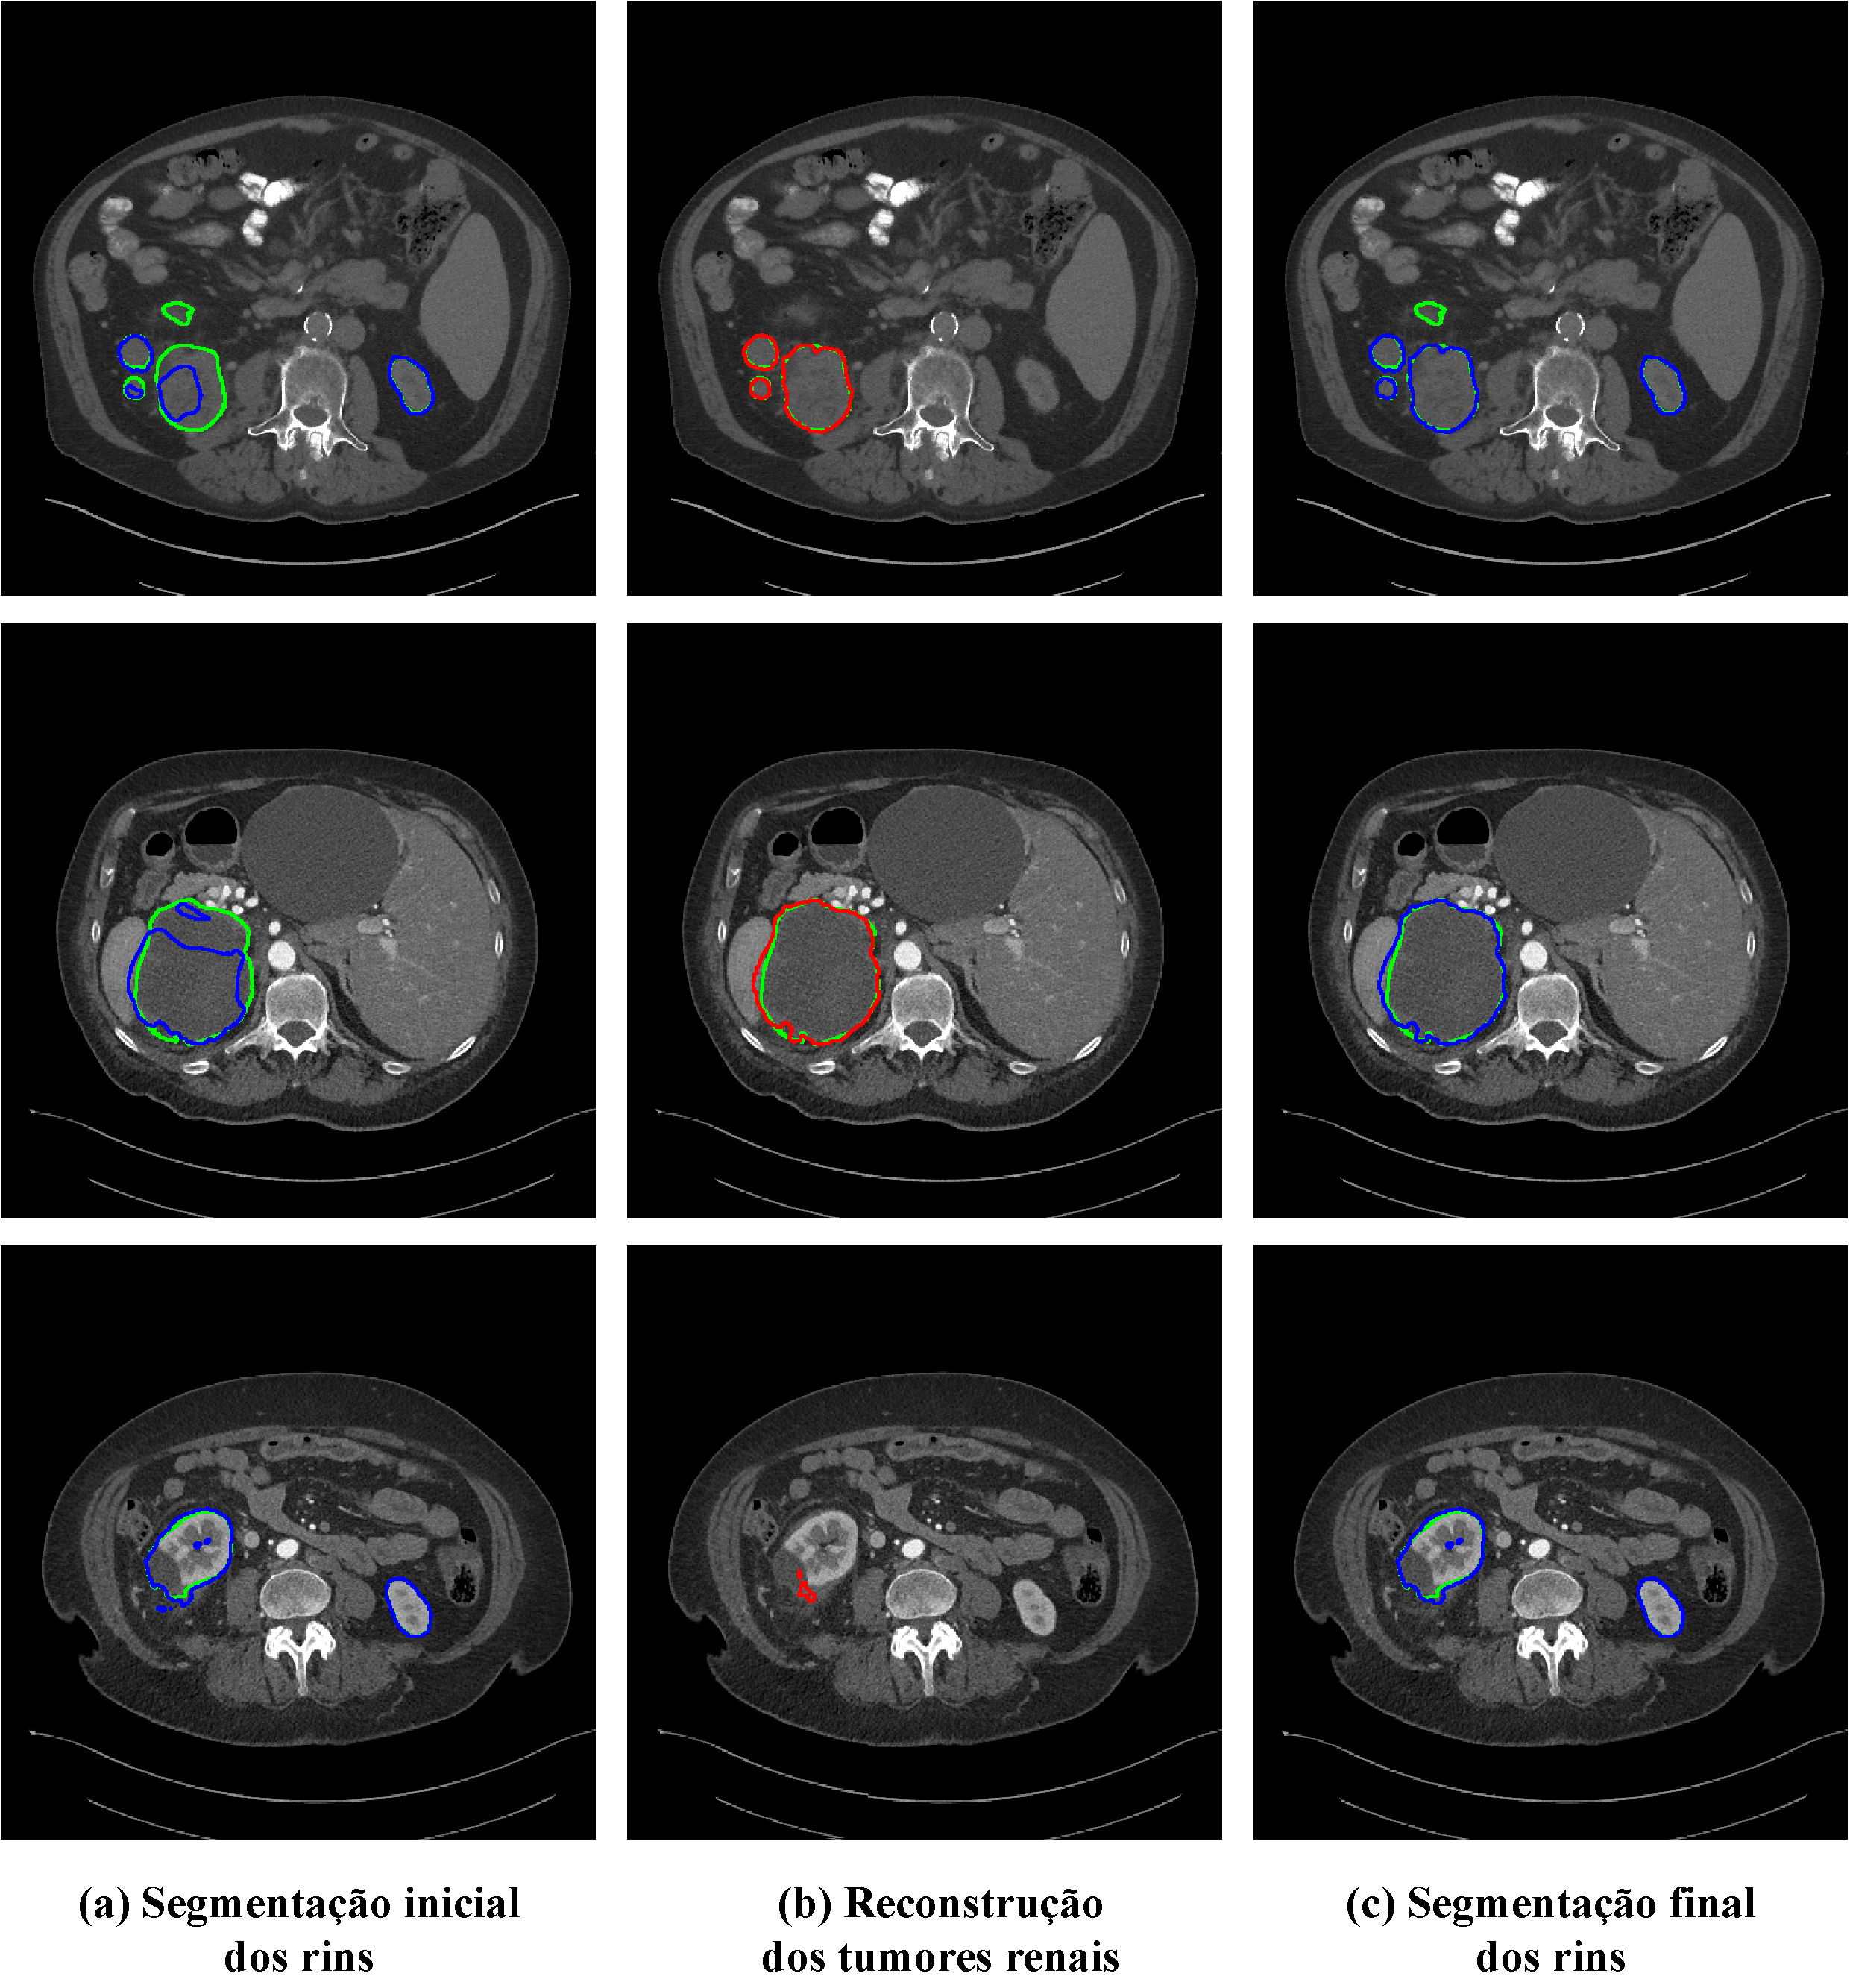
\includegraphics[width=0.98\textwidth]{figuras/res-seg-rins-final.pdf}
    \label{fig:res-final-rins}
    \legend{Fonte: Elaborado pela autora.}
\end{figure}

Vale destacar o último caso (imagens inferiores), em que alguns falsos positivos segmentados foram observados na etapa inicial de segmentação renal (Figura~\ref{fig:res-final-rins} (a) inferior). No entanto, foram removidos após a aplicação do pós-processamento (manter os dois maiores elementos). Portanto, acredita-se que este conjunto de etapas seja capaz de contribuir para melhorar o resultado da segmentação de rins.


%Observando a etapa de manter apenas o maior objeto, garante-se uma melhora em relação ao Dice e especificidade, ou seja, há menos falsos positivos e uma segmentação mais precisa. Apesar de haver uma perda na sensibilidade, vale lembrar que as métricas são medidas por pixels, ou seja, existem mais números de pixels pertencentes a classe de não esôfago do que esôfago, então qualquer melhora na especificidade (acertar os casos negativos) melhora significativamente o valor de Dice.

\subsection{Redução de Falsos Positivos para os Tumores Renais}
\label{sec:resultados-reducao-falsos-positivos-tumores-renais}

Esta etapa completa o método proposto para segmentação de tumores renais. Para isso, são usadas as segmentações das etapas anteriores obtidas, conforme descrito na Seção~\ref{sec:resultados-reducao-falsos-positivos-rins}. Com as segmentações obtidas, foi feita a intersecção da segmentação final dos rins com a etapa de reconstrução dos tumores renais para extrair apenas a região que contém os tumores, removendo assim parte dos falsos positivos adquiridos na reconstrução dos tumores. Finalmente, os resultados dessa etapa são passados pela etapa de pós-processamento para reduzir os falsos positivos que não foram removidos na etapa anterior. 

O pós-processamento consistiu na remoção de estruturas segmentadas sem informação contextual suficiente para representar as regiões dos tumores renais, ou seja, elementos com menos de três fatias contínuas (Seção~\ref{sec:metodo-reducao-falsos-positivos-tumores-renais}). Os resultados após o pós-processamento estão descritos na Tabela~\ref{tab:seg-final-tumores-renais}. A segmentação final atingiu 84,06\% de Dice, 75,04\% de Jaccard, 99,94\% de acurácia, 88,33\% de sensibilidade e 99,95\% de especificidade.

\begin{table}[!ht]
\caption{Resultados da etapa de segmentação final dos tumores renais.}
\label{tab:seg-final-tumores-renais}
\centering
\begin{tabular}{c|c|c|c|c|c}
\hline
Resultado Final  & Dice(\%)                      & Jacc(\%)                      & Acc(\%) & Sen(\%)                       & Esp(\%) \\ \hline
2D               & 73,62                          & 61,21                          & 99,89    & 81,03                          & 99,91    \\ \hline
2.5D             & 84,06                          & 75,04                          & 99,94    & 88,33                          & 99,95    \\ \hline
\textit{P-value} & \cellcolor[HTML]{C0C0C0}0,0000 & \cellcolor[HTML]{C0C0C0}0,0000 & 0,3680   & \cellcolor[HTML]{C0C0C0}0,0000 & 0,4275   \\ \hline
\end{tabular}
\end{table}

Em termos estatísticos, a segmentação final dos tumores renais usando as abordagens 2D e 2.5D apresentou um \textit{p-value} igual a 0 para as métricas Dice, Jaccard e sensibilidade. Portanto, comprova que existe uma diferença significativa entre as segmentações finais, visto que a hipótese nula foi rejeitada. Isso demonstra que as segmentações finais usando a abordagem 2.5D são mais precisas, com menos falsos positivos e mais regiões de tumores. Uma vez que, as métricas descritas (Dice, Jaccard e sensibilidade) indicam a capacidade de identificar regiões de tumores e a semelhança entre os objetos em estudo.

Além disso, pode-se observar que houve melhorias consideráveis nas métricas Dice, Jaccard e sensibilidade em relação às segmentações iniciais dos candidatos a tumores renais (Seção~\ref{sec:resultados-candidatores-tumores-renais-regiao-renal} e~\ref{sec:resultados-candidatores-tumores-renais-regiao-abdominal}). Isso comprova a importância das etapas anteriores para a obtenção de resultados expressivos. Portanto, devido à melhora significativa nos resultados finais, o trabalho dos especialistas para analisar todos os elementos segmentados é reduzido.

Três casos aplicando as etapas para obter a segmentação final dos tumores renais são apresentados na Figura~\ref{fig:res-final-tumores-renais}. Primeiramente, pode-se observar que a segmentação de candidatos a tumores renais na região renal (Figura~\ref{fig:res-final-tumores-renais} (a)) não foi capaz de segmentar com precisão as regiões dos tumores. Além disso, muitas regiões renais não foram segmentadas na etapa de segmentação inicial dos rins, o que acabou comprometendo o desempenho do modelo, uma vez que ficou impossibilitado de segmentar mais regiões tumorais. No entanto, a etapa de segmentação de candidatos a tumores renais na região abdominal (Figura~\ref{fig:res-final-tumores-renais} (b)) compensa a deficiência da segmentação inicial dos rins e candidatos a tumores renais na região renal, permitindo a segmentação de mais regiões tumorais. Isso é possível porque esta etapa analisa mais informações contextuais em uma região mais ampla (abdominal). 

\begin{figure}[!ht]
    \centering
    \caption{Etapas da segmentação dos tumores renais. Marcação do especialista (verde) e segmentação do método (vermelho).}
    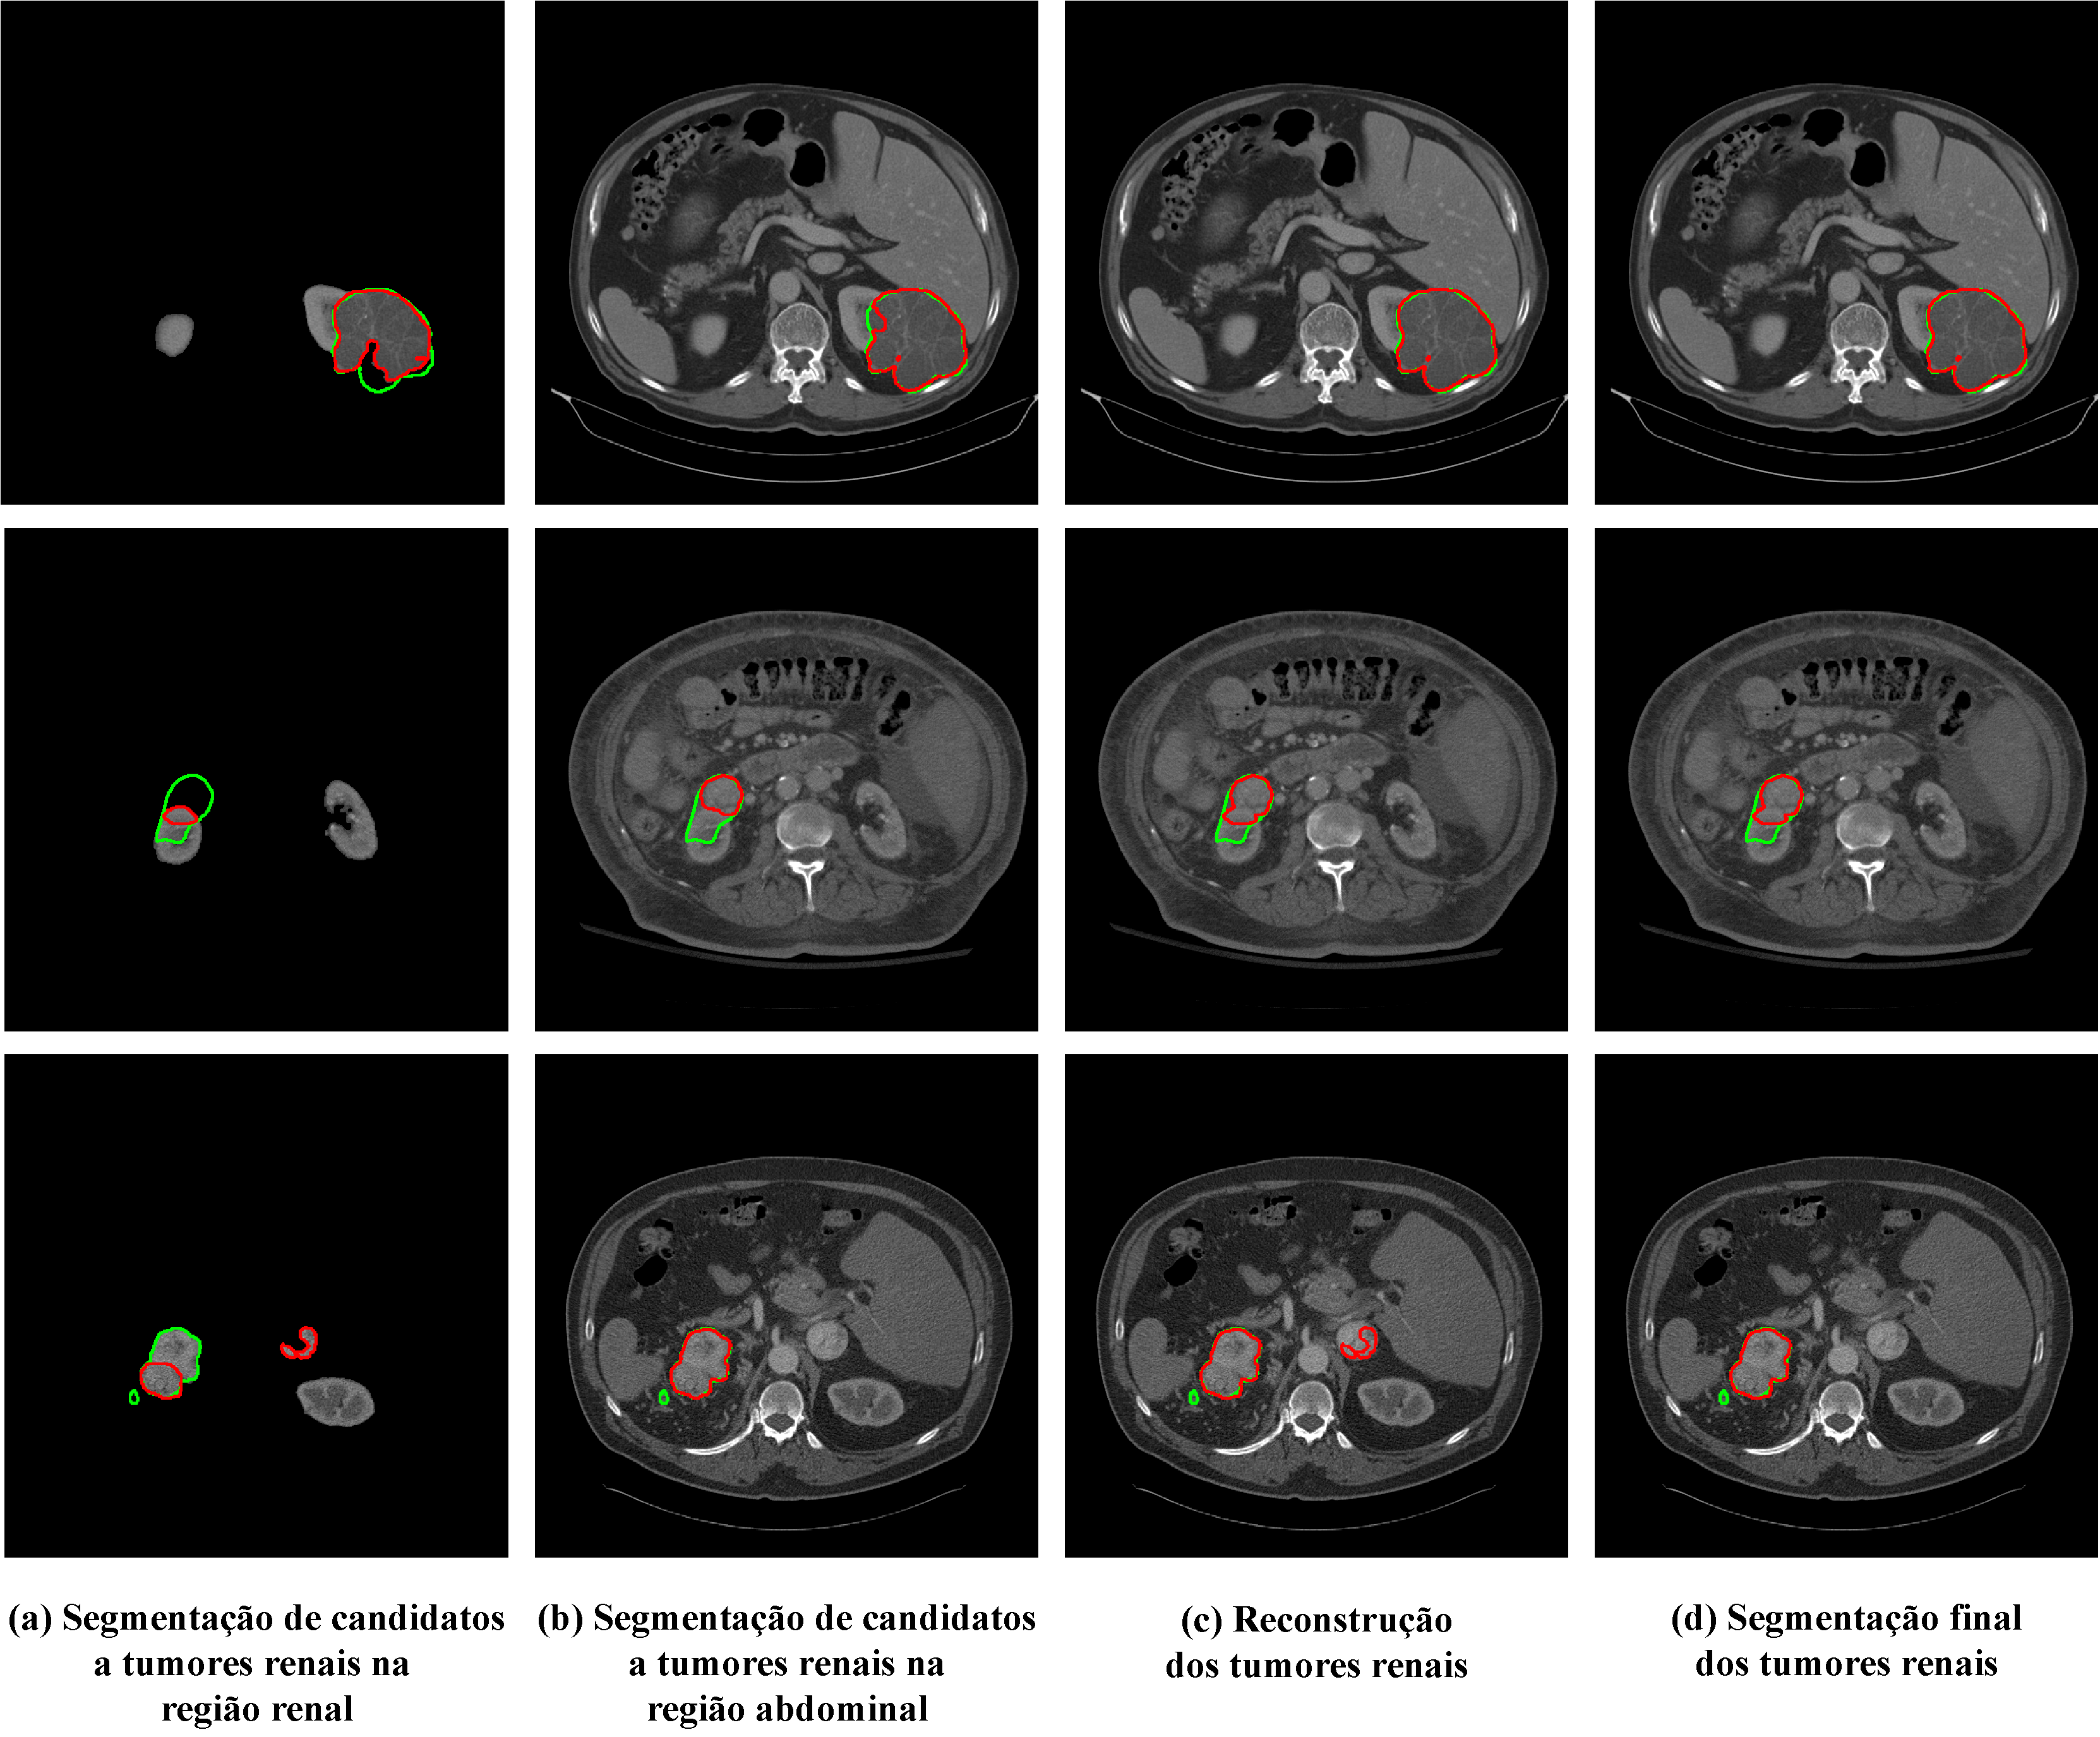
\includegraphics[width=1\textwidth]{figuras/res-seg-tumores-renais-final.pdf}
    \label{fig:res-final-tumores-renais}
    \legend{Fonte: Elaborado pela autora.}
\end{figure}
\FloatBarrier

Posteriormente, a etapa de reconstrução de tumores renais (Figura~\ref{fig:res-final-tumores-renais} (c)) combinou as etapas de segmentação de candidatos a tumores renais na região renal e abdominal. Isso levou a uma segmentação mais precisa da região tumoral, pois regiões tumorais não segmentadas no primeiro estágio foram segmentadas no segundo estágio, agregando os resultados. Finalmente, a segmentação final dos tumores é mostrada na Figura~\ref{fig:res-final-tumores-renais} (d). Pode-se analisar que mais tecidos das regiões tumorais foram incluídos devido à etapa de reconstrução do tumor.

Por fim, vale destacar o último caso (imagens inferiores) da Figura~\ref{fig:res-final-tumores-renais}. No qual pode-se observar que na etapa de segmentação dos candidatos a tumores renais na região renal (Figura~\ref{fig:res-final-tumores-renais} (a) inferior), as regiões tumorais foram segmentadas, mas também falsos positivos. Entretanto, foram eliminados após a aplicação do pós-processamento (remoção de elementos descontínuos). Portanto, acredita-se que todas as etapas foram importantes para melhorar a segmentação dos tumores.

\subsection{Método Proposto com/sem Balanceamento de Fatias}
\label{sec:com-sem-balanceamento-fatias}

Após os experimentos usando abordagens 2D e 2.5D, foram realizados mais alguns experimentos para validar as demais etapas do método proposto. Primeiramente, foi verificada a eficácia da técnica de balanceamento de fatias no conjunto de treinamento e validação. Para isso, foi realizado um experimento com e sem balanceamento de fatias no método proposto, no qual, ao invés de usar a estratégia de balanceamento de fatias, os modelos foram treinados e validados usando todas as fatias dos volumes de TCs. Posteriormente, todas as outras etapas do método proposto foram aplicadas com base neste experimento. Os resultados finais do método proposto com e sem balanceamento proporcional são apresentados na Tabela~\ref{tab:com-sem-balanceamento}. Além disso, é mostrado o tempo de treinamento para cada época dos modelos (ResUNet 2.5D e DeepLabv3+ 2.5D). Na segmentação dos tumores renais é apresentado o resultado da soma dos tempos de treinamento dos modelos para segmentar candidatos a tumores renais na região renal e abdominal.

\begin{table}[!ht]
\caption{Resultado do método proposto com/sem balanceamento de fatias.}
\label{tab:com-sem-balanceamento}
\doublespacing
\centering
\resizebox{\columnwidth}{!}{
\begin{tabular}{cl|c|c|c|c|c|c}
\hline
\multicolumn{1}{c|}{Segmentação}                                                                                 & \multicolumn{1}{c|}{Técnica} & Dice(\%)                      & Jacc(\%)                      & Acc(\%) & Sen(\%)                       & Esp(\%) & T. por época \\ \hline
\multicolumn{1}{l|}{}                                                                                            & Todas as fatias              & 43,79                          & 32,11                          & 99,63    & 77,00                          & 99,65    & -            \\ \cline{2-8} 
\multicolumn{1}{l|}{\multirow{-2}{*}{\begin{tabular}[c]{@{}l@{}}Reconstrução dos\\ Tumores Renais\end{tabular}}} & Balanceado                   & 68,20                          & 57,17                          & 99,90    & 90,33                          & 99,91    & -            \\ \hline
\multicolumn{1}{c|}{}                                                                                            & Todas as fatias              & 92,96                          & 87,38                          & 99,84    & 93,05                          & 99,92    & 1h 01m 52s            \\ \cline{2-8} 
\multicolumn{1}{c|}{\multirow{-2}{*}{Rins}}                                                                      & Balanceado                   & 97,45                          & 95,05                          & 99,95    & 98,44                          & 99,96    & 33m 29s            \\ \hline
\multicolumn{1}{c|}{}                                                                                            & Apenas fatias com rins       & 62,03                          & 49,15                          & 99,82    & 75,99                          & 99,85    & 46m 03s            \\ \cline{2-8} 
\multicolumn{1}{c|}{\multirow{-2}{*}{Tumores Renais}}                                                            & Balanceado                   & 84,06                          & 75,04                          & 99,94    & 88,33                          & 99,95    & 24m 33s            \\ \hline
\multicolumn{2}{c|}{\textit{P-value}}                                                                                                           & \cellcolor[HTML]{C0C0C0}0,0000 & \cellcolor[HTML]{C0C0C0}0,0000 & 0,0690   & \cellcolor[HTML]{C0C0C0}0,0000 & 0,0969   & -            \\ \hline
\end{tabular}
}
\end{table}

Pode-se observar que a abordagem proposta com balanceamento de fatias produz melhorias significativas em todas as colunas em comparação com a abordagem sem balanceamento de fatias. Inclusive o tempo com balanceamento é inferior, pois tem menos fatias que a abordagem sem balanceamento. Analisando a métrica sensibilidade entre as abordagens, pode-se verificar que sofreu um impacto negativo em relação à abordagem com balanceamento de fatias. Isso acontece porque, sem aplicar o balanceamento de fatias, os modelos terão como entrada mais fatias de fundo (sem rim, sem tumores, dependendo do modelo) do que fatias com o objeto de interesse (rins ou tumores). Dessa forma, o modelo tende a aprender mais fatias de fundo e não consegue segmentar com precisão o objeto de interesse, portanto, o modelo tem baixa sensibilidade e, consequentemente, resultados baixos para Dice e Jaccard.

Além disso, estatisticamente, obteve-se um \textit{p-value} de 0,0034 na acurácia em relação à reconstrução de tumores e um \textit{p-value} igual a 0 para as métricas Dice, Jaccard e sensibilidade em relação a todas as abordagens com/sem balanceamento de fatias e, portanto, a hipótese nula foi rejeitada. Portanto, com os resultados experimentais foi possível comprovar que a técnica de balanceamento de fatias é fundamental para a obtenção de resultados mais consistentes na segmentação dos rins e segmentação e reconstrução de tumores renais. Essa melhora se deve à capacidade do balanceamento detectar fatias com e sem tumores, possibilitando segmentar mais regiões de interesse e minimizar falsos positivos.

%-- Reconstrução de tumores 0,0034 acurácia

\subsection{Método Proposto com Distribuição Aleatória e Proporcional da Base de Imagens}
\label{sec:distribuicao-proporcional-grupos-tumores}

O próximo experimento realizado foi relacionado a etapa da distribuição proporcional da base de imagens. Para validar essa etapa, o conjunto de teste permaneceu o mesmo e os modelos de segmentação e reconstrução foram treinados com outro conjunto de treino e validação distribuídos aleatoriamente. As demais etapas do método proposto foram aplicadas posteriormente. Os resultados finais do método proposto com distribuição aleatória e proporcional são apresentados na Tabela~\ref{tab:aleatorio-distribuidos}. Também são apresentados o tempo de treinamento para cada época dos modelos (ResUNet 2.5D e DeepLabv3+ 2.5D). Na segmentação dos tumores renais, é apresentado o resultado da soma dos tempos de treinamento dos modelos para segmentar candidatos a tumores renais na região renal e abdominal.

\begin{table}[!ht]
\caption{Resultado do método proposto com distribuição aleatória e proporcional.}
\label{tab:aleatorio-distribuidos}
\doublespacing
\centering
\resizebox{\columnwidth}{!}{
\begin{tabular}{cl|c|c|c|c|c|c}
\hline
\multicolumn{1}{c|}{Segmentação}                                                                                 & \multicolumn{1}{c|}{Técnica} & Dice(\%)                      & Jacc(\%)                      & Acc(\%) & Sen(\%)                       & Esp(\%) & T. por época \\ \hline
\multicolumn{1}{l|}{}                                                                                            & Aleatório                    & 53,39                          & 40,78                          & 99,78    & 82,22                          & 99,81    & -            \\ \cline{2-8} 
\multicolumn{1}{l|}{\multirow{-2}{*}{\begin{tabular}[c]{@{}l@{}}Reconstrução dos\\ Tumores Renais\end{tabular}}} & Distribuição proporcional    & 68,20                          & 57,17                          & 99,90    & 90,33                          & 99,91    & -            \\ \hline
\multicolumn{1}{c|}{}                                                                                            & Aleatório                    & 94,18                          & 90,06                          & 99,90    & 94,44                          & 99,95    & 34m 33s            \\ \cline{2-8} 
\multicolumn{1}{c|}{\multirow{-2}{*}{Rins}}                                                                      & Distribuição proporcional    & 97,45                          & 95,05                          & 99,95    & 98,44                          & 99,96    & 33m 29s            \\ \hline
\multicolumn{1}{c|}{}                                                                                            & Aleatório                    & 71,29                          & 59,17                          & 99,89    & 80,64                          & 99,91    & 27m 14s           \\ \cline{2-8} 
\multicolumn{1}{c|}{\multirow{-2}{*}{Tumores Renais}}                                                            & Distribuição proporcional    & 84,06                          & 75,04                          & 99,94    & 88,33                          & 99,95    & 24m 33s             \\ \hline
\multicolumn{2}{c|}{\textit{P-value}}                                                                                                           & \cellcolor[HTML]{C0C0C0}0,0000 & \cellcolor[HTML]{C0C0C0}0,0000 & 0,1152   & \cellcolor[HTML]{C0C0C0}0,0000 & 0,1605   & -            \\ \hline
\end{tabular}
}
\end{table}

A partir dos resultados obtidos, é possível ver a importância da etapa de distribuição proporcional, não só por ter obtido resultados melhores do que com a aplicação da distribuição aleatória, mas também por atingir um \textit{p-value} igual a 0 para várias métricas (Dice, Jaccard e sensibilidade), revelando-se significativamente diferentes. Portanto, esta etapa garante que os modelos sejam equilibrados e obtenham um melhor desempenho, além de ser importante para o sucesso das demais etapas do método proposto.

\subsection{Segmentação de Rins sem/com a Etapa de Reconstrução de Tumores Renais}
\label{sec:segmentacao-rins-sem-reconstrucao-tumoral}

Neste experimento, o foco foi avaliar a etapa de reconstrução de tumores renais do método proposto para segmentação de rins. Basicamente, a etapa de reconstrução tumoral foi excluída para verificar o impacto nos resultados da segmentação renal. Vale ressaltar que todas as configurações experimentais e demais etapas foram aplicadas. Os resultados são apresentados na Tabela~\ref{tab:res-segmentacao-rins-sem-reconstrucao-tumoral}.

\begin{table}[!ht]
\caption{Resultados da segmentação de rins com e sem a etapa de reconstrução tumoral.}
\label{tab:res-segmentacao-rins-sem-reconstrucao-tumoral}
\centering
\onehalfspacing
\resizebox{\columnwidth}{!}{
\begin{tabular}{c|c|c|c|c|c}
\hline
Segmentação de Rins                & Dice(\%) & Jacc(\%) & Acc(\%) & Sen(\%)                       & Esp(\%) \\ \hline
Sem Reconstrução de Tumores Renais & 97,11     & 94,44     & 99,94    & 97,57                          & 99,97    \\ \hline
Com Reconstrução de Tumores Renais & 97,45     & 95,05     & 99,95    & 98,44                          & 99,96    \\ \hline
\textit{P-value}                   & 0,2794    & 0,1550    & 0,8767   & \cellcolor[HTML]{C0C0C0}0,0011 & 0,9375   \\ \hline
\end{tabular}
}
\end{table}

Analisando os resultados das métricas de avaliação, pode-se notar que os melhores resultados da segmentação de rins é aplicando também a etapa de reconstrução tumoral. Essa etapa é capaz de recuperar regiões consideráveis de tumores, que por sua vez também são regiões renais e possivelmente não foram inicialmente segmentadas. Portanto, ao aplicar a reconstrução tumoral, as regiões renais também são reconstruídas, delimitando melhor os contornos renais. Estatisticamente, obteve-se um \textit{p-value} de 0,0011 para a métrica de sensibilidade em relação às abordagens comparadas. Isso significa que o uso da etapa de reconstrução tumoral tem impacto positivo na obtenção de mais regiões da classe positiva (rins). Portanto, acredita-se que essa etapa é válida para obter resultados mais precisos para a segmentação renal.

\subsection{Segmentação de Tumores Renais aplicando a Máscara do Método/Especialista}
\label{sec:segmentacao-tumores-mascara-metodo-especialista}

No último experimento, a segmentação de tumores renais foi analisada usando diferentes abordagens de imagens de entrada para o método. Para validar isso, apenas as formas de entrada para a segmentação de candidatos a tumores renais na região renal foram usadas para estudo. As demais etapas não foram utilizadas para não causar impacto no estudo avaliado em questão. Portanto, o objetivo deste experimento é investigar o impacto da segmentação de tumores quando a máscara renal marcada pelo especialista é aplicada como entrada da rede e como as demais etapas são refletidas.

\begin{table}[!ht]
\caption{Resultados da segmentação de tumores renais aplicando a máscara do método e do especialista.}
\label{tab:res-segmentacao-tumores-mascara-metodo-especialista}
\centering
\onehalfspacing
\resizebox{\columnwidth}{!}{
\begin{tabular}{c|c|c|c|c|c}
\hline
Segmentação de Tumores Renais & Dice(\%)                      & Jacc(\%)                      & Acc(\%) & Sen(\%)                       & Esp(\%) \\ \hline
Máscara do Especialista       & 84,95                          & 75,06                          & 99,68    & 84,44                          & 99,80    \\ \hline
Máscara do Método             & 81,02                          & 69,66                          & 99,93    & 80,52                          & 99,97    \\ \hline
\textit{P-value}              & \cellcolor[HTML]{C0C0C0}0,0010 & \cellcolor[HTML]{C0C0C0}0,0001 & 0,0738   & \cellcolor[HTML]{C0C0C0}0,0011 & 0,1136   \\ \hline
\end{tabular}
}
\end{table}

As duas abordagens avaliadas foram: aplicar a máscara proveniente da segmentação inicial dos rins (etapa anterior) como entrada da rede; e usar a máscara renal marcada pelo especialista como entrada da rede. Os resultados dessas abordagens são apresentados na Tabela~\ref{tab:res-segmentacao-tumores-mascara-metodo-especialista}. É perceptível que os resultados usando como entrada da rede a máscara do especialista apresentaram resultados superiores. Além disso, em termos estatísticos também comprovam que as abordagens são significativamente diferentes.

A partir disto, é possível tirar conclusões sobre a segmentação inicial dos rins obtida pelo método proposto. Em que, embora 96,37\% de Dice seja obtido na segmentação inicial dos rins (Tabela~\ref{tab:seg-inicial-rins}), partes de regiões renais que também são tumores não são segmentadas. Portanto, usando a máscara dos rins da segmentação inicial dos rins, não foi possível segmentar maiores regiões tumorais devido à perda de regiões renais. No entanto, resultados superiores foram produzidos aplicando a máscara do especialista ao mesmo modelo de segmentação (DeepLabv3+ 2.5D). Portanto, é possível concluir que o modelo de segmentação de tumores apresenta bom desempenho, pois o que causa resultados inferiores é somente quando as regiões renais que possuem tumores não são visíveis como áreas para segmentação.

Entretanto, é importante destacar que a deficiência da segmentação de rins é suprida com as demais etapas do método proposto. Em que as regiões não segmentadas inicialmente são reconstruídas usando a etapa de reconstrução dos tumores renais. Mediante isso, os resultados finais para a segmentação de tumores (84,06\% de Dice, na Tabela~\ref{tab:seg-final-tumores-renais}) são equiparáveis aos resultados quando não há perda de regiões renais/tumorais. Mais uma vez, é notável como as etapas do método proposto são essenciais e robustas, o que acaba impactando nos bons resultados para a segmentação de rins e tumores.

%A partir disto, é possível tirar conclusões sobre a qualidade da segmentação de rins obtida pelo método proposto e verificar as demais etapas para suprir possíveis deficiências da segmentação de rins.

\section{Diversos Experimentos Testados}
\label{sec:experimentos-testados}

Finalmente, esta última seção descreve um resumo dos principais experimentos realizados na elaboração do método proposto. A Tabela~\ref{tab:diversos-experimentos} apresenta o resumo dos principais pré-processamentos, arquiteturas, codificadores e abordagens aplicadas. Os diversos experimentos foram aplicados em diferentes etapas do método e foram feitas combinações entre eles.

\begin{table}[!ht]
\caption{Resumo dos diversos experimentos testados.}
\label{tab:diversos-experimentos}
\centering
\onehalfspacing
\resizebox{\columnwidth}{!}{
\begin{tabular}{c|c|c|c}
\hline
Pré-processamentos                                                                                               & Arquiteturas                                                                                               & Codificadores                                                                                                                                                                                        & Abordagens                                                            \\ \hline
\begin{tabular}[c]{@{}c@{}}CLAHE, bilateral, média,\\ equalização do histograma\\ e unsharp masking\end{tabular} & \begin{tabular}[c]{@{}c@{}}UNet, UNet++,\\ DeepLabv3, DenseUNet\\ e Pyramid Attention Network\end{tabular} & \begin{tabular}[c]{@{}c@{}}AlexNet, DenseNet, ResNet-18,\\ ResNet-34, ResNet-50, ResNet-152,\\ ResNeXt, SqueezeNet, Xception,\\ Inception, DPN-98, EfficientNet-B3\\ e EfficientNet-B7\end{tabular} & \begin{tabular}[c]{@{}c@{}}2D, 2.5D\\ (com 5 e 7 fatias)\end{tabular} \\ \hline
\end{tabular}
}
\end{table}

Na primeira coluna, podem ser vistos os principais pré-processamentos que foram aplicados na etapa inicial do método proposto. Todos eles foram testados individualmente e em conjunto com o objetivo de melhorar as imagens usadas no método, visando aprimorar o desempenho de segmentação. A segunda coluna contém as arquiteturas de rede que foram testadas para segmentação de rins e candidatos a tumores renais, nas quais pode-se observar que foram usadas desde arquiteturas clássicas como a U-Net até arquiteturas de última geração como DeepLabv3 e \textit{Pyramid Attention Network}~\cite{li2018pyramid}. A terceira coluna mostra os codificadores que foram testados nas arquiteturas descritas.

A última coluna, mostra as abordagens 2D e 2.5D. No caso da abordagem 2.5D, foram testados com 5 e 7 fatias. \textit{O data augmentation offline} também foi testado, mas desvantagens como memória e tempo de treinamento adicionais e alto custo computacional foram encontrados. De qualquer forma, \textit{data augmentation online} apresentou resultados superiores com baixo custo computacional em relação aos outros. Por fim, é importante destacar que para cada um dos experimentos foram aplicadas diversas combinações entre eles. Em geral, como pode ser visto, durante o desenvolvimento do método proposto atual uma série de testes foram realizados. No entanto, os experimentos descritos não superaram os resultados atuais, apresentando resultados inferiores a 90,12\% e 66,7\% de Dice na segmentação de rins e tumores, respectivamente, levando-se em consideração a melhor combinação.

\section{Considerações Finais}
\label{considerações-finais-resultados}

Neste capítulo, os resultados obtidos pelos experimentos realizados no desenvolvimento do método proposto foram apresentados e discutidos. Além disso, mais alguns experimentos foram realizados a fim de validar as etapas do método proposto.

No próximo capítulo serão apresentados os estudos de casos, também será feita uma comparação com os trabalhos descritos na literatura, visando contextualizar a relevância da pesquisa desenvolvida neste trabalho. Por fim, serão descritos os principais aspectos e limitações encontrados após a análise das etapas propostas.

% estudo de caso 1: RA; estudo de caso 2: RV;
\chapter{Discussão}
\label{cap:discussao}
\phantom{0}

Este capítulo apresentada vários estudos de caso, bem como uma comparação do método proposto com os trabalhos relacionados encontrados na literatura (Capítulo~\ref{cap:trabalhos-relacionados}). Por fim, são discutidas as vantagens e limitações do método.

\section{Estudos de Caso – Segmentação de Rins}
\label{sec:estudos-segmentacao-rins}

Esta seção apresenta um conjunto de estudos de caso para analisar a influência das etapas propostas na segmentação de rins. Os casos observados foram: (1) a segmentação inicial apresentou uma segmentação precisa e as demais etapas não foram necessárias; (2) as etapas de reconstrução dos tumores renais e pós-processamento reduziram ligeiramente o desempenho da segmentação inicial; e (3) as etapas de reconstrução de tumores renais e pós-processamento foram necessárias e capazes de melhorar a qualidade da segmentação inicial.

\subsection{Estudo de Caso 1 – Paciente case\_00018}
\label{sec:estudo-rins-1}

O primeiro estudo de caso trata de um exame em que as etapas de reconstrução e pós-processamento dos tumores foram desnecessárias. Este caso é ilustrado na Figura~\ref{fig:estudo-rins-1}, onde pode-se ver que nenhum fragmento segmentado está presente, exceto os rins. Além disso, é notável que a etapa de reconstrução dos tumores renais (Figura~\ref{fig:estudo-rins-1}~(c), em cinza a segmentação inicial dos rins e em verde a reconstrução dos tumores renais) não contribuiu para uma maior segmentação na região renal, uma vez que as regiões reconstruídas dos tumores renais já haviam sido segmentadas na etapa inicial (dentro do rim). A segmentação dos rins obteve 94,67\% Dice, 89,88\% Jaccard, 99,91\% de acurácia, 99,88\% de sensibilidade e 99,91\% de especificidade. Após as etapas de reconstrução e pós-processamento (Figura~\ref{fig:estudo-rins-1} (d)) dos tumores, os resultados permaneceram os mesmos. Portanto, a segmentação inicial foi capaz de determinar contornos renais muito precisos. Esse tipo de comportamento foi encontrado em 4 pacientes.

\begin{figure}[!ht]
    \centering
    \caption{Estudo de caso 1. Segmentações dos rins (cinza) e reconstrução dos tumores renais (verde).}
    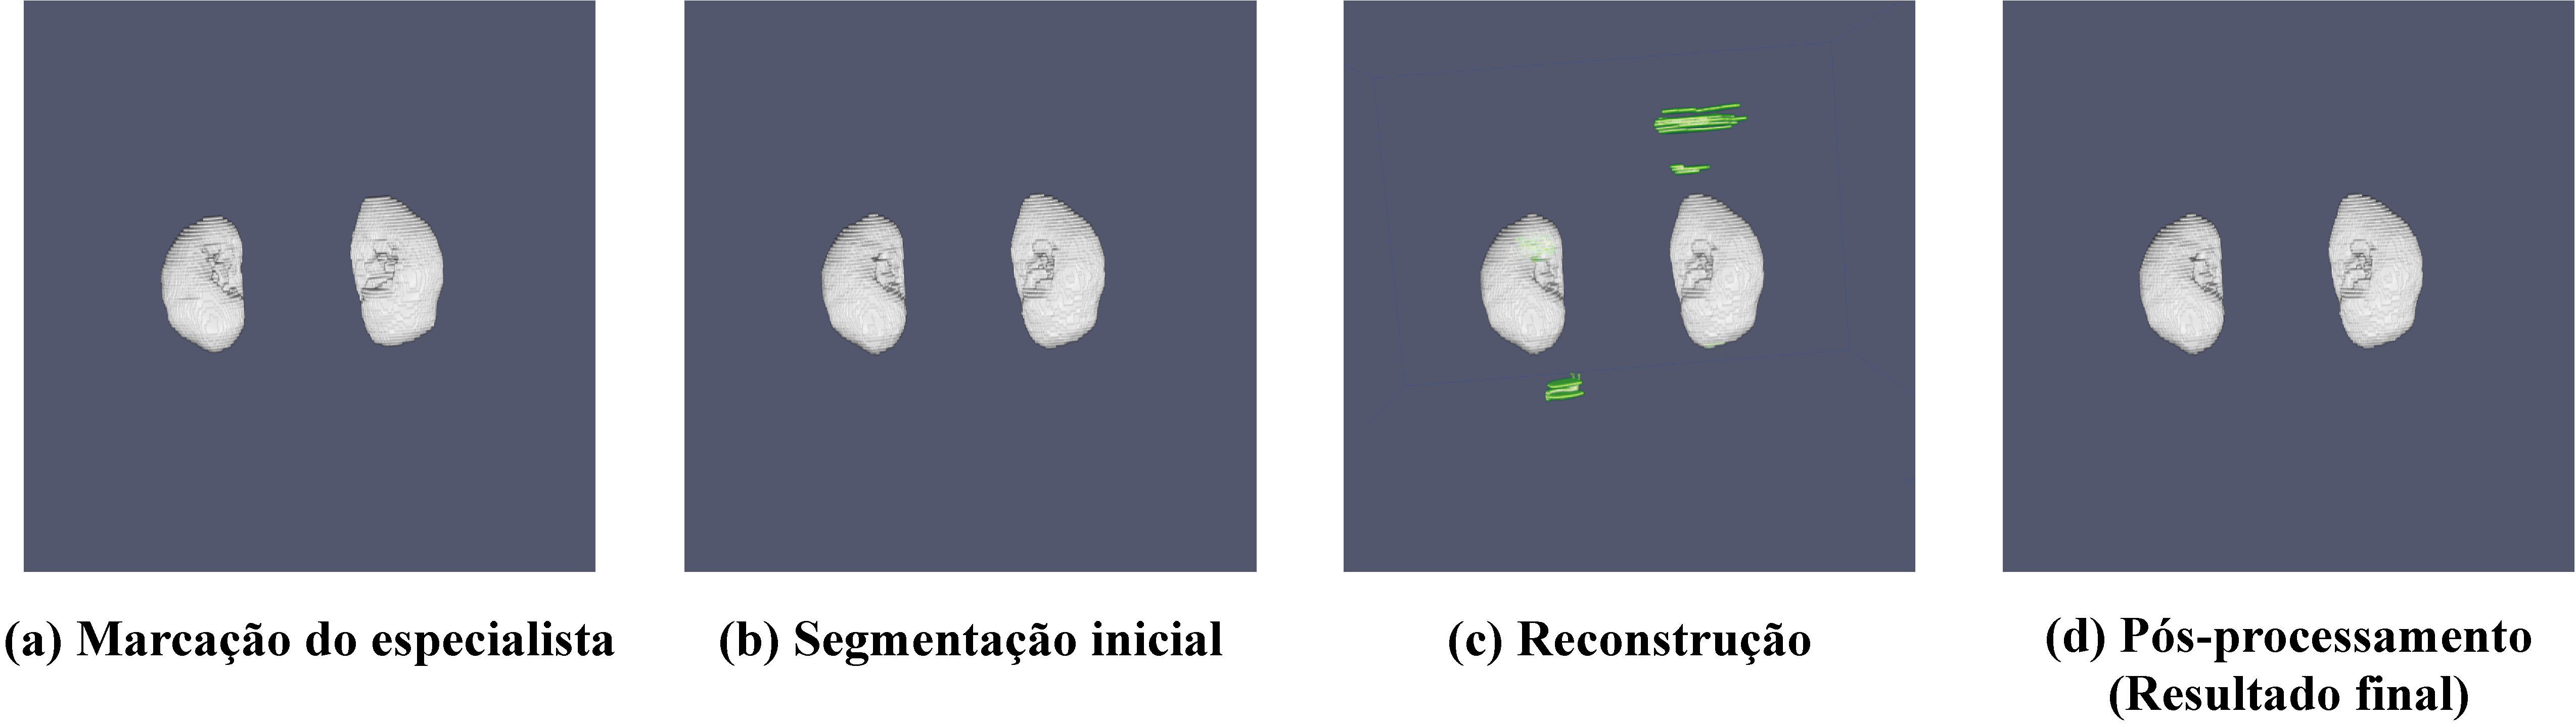
\includegraphics[width=1\textwidth]{figuras/estudos-casos-rins-1-18.pdf}
    \label{fig:estudo-rins-1}
    \legend{Fonte: Elaborado pela autora.}
\end{figure}

\subsection{Estudo de Caso 2 – Paciente case\_00149}
\label{sec:estudo-rins-caso-2}

Neste estudo de caso, as etapas de reconstrução e pós-processamento dos tumores afetaram sutilmente a segmentação inicial. Pode-se ver na Figura~\ref{fig:estudo-rins-2} que a combinação das etapas descritas não foi capaz de melhorar os resultados da segmentação inicial. A etapa mais crítica foi a reconstrução de tumores renais (Figura~\ref{fig:estudo-rins-2} (c)), na qual é possível observar que comprometeu a região renal com mais fragmentos de falsos positivos. A segmentação inicial obteve 98,48\% Dice, 97,00\% Jaccard, 99,95\% de acurácia, 98,37\% de sensibilidade e 99,98\% de especificidade e a segmentação final (reconstrução + pós-processamento) obteve 98,37\% Dice, 96,79\% Jaccard, 99,94\% de acurácia, 98,50\% de sensibilidade e 99,97\% de especificidade. Apesar disso, as taxas de desempenho da maioria dos quantificadores não foram tão afetadas. Esse tipo de comportamento foi encontrado em apenas 2 pacientes.

\begin{figure}[!ht]
    \centering
    \caption{Estudo de caso 2. Segmentações dos rins (cinza) e reconstrução dos tumores renais (verde).}
    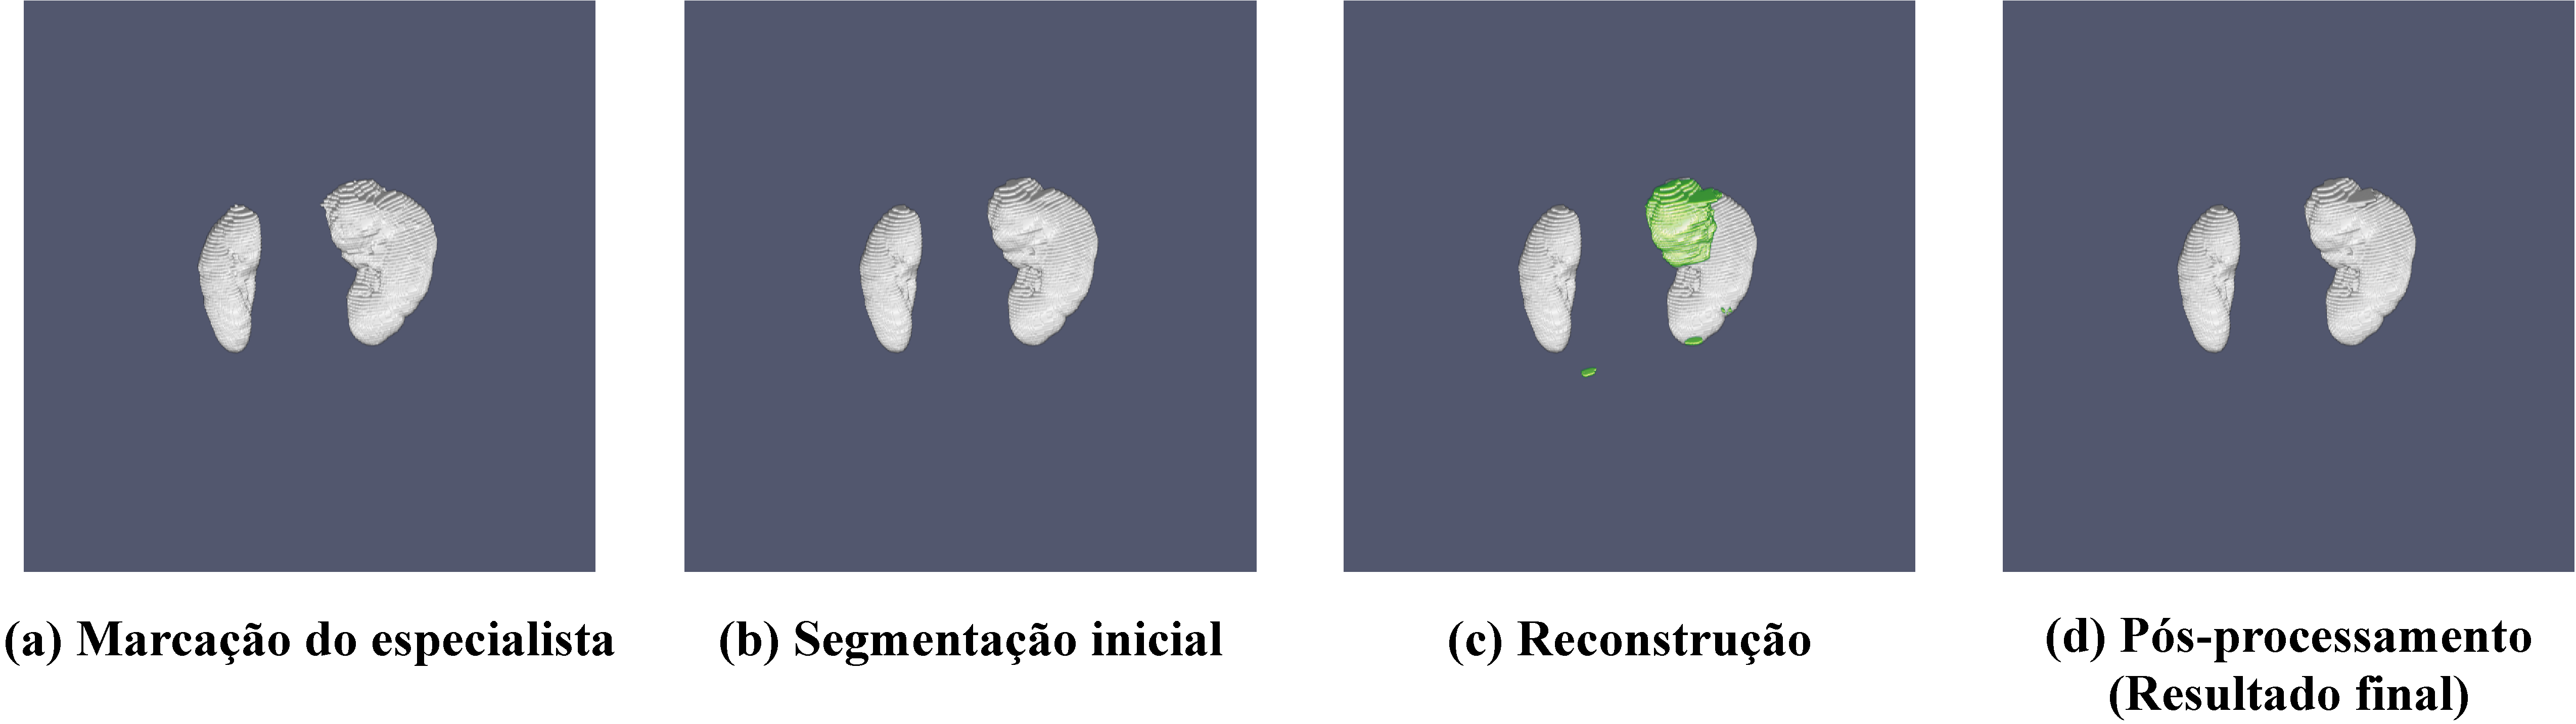
\includegraphics[width=1\textwidth]{figuras/estudos-casos-rins-2-149.pdf}
    \label{fig:estudo-rins-2}
    \legend{Fonte: Elaborado pela autora.}
\end{figure}

\subsection{Estudo de Caso 3 – Paciente case\_00045}
\label{sec:estudo-rins-caso-3}

No último estudo de caso dos rins, as etapas de reconstrução e pós-processamento dos tumores funcionaram bem. É possível ver na Figura~\ref{fig:estudo-rins-3} que a segmentação inicial dos rins gerou alguns fragmentos errôneos (falsos positivos). Além disso, algumas regiões renais não foram segmentadas, porém a reconstrução dos tumores renais foi capaz de suprir essa deficiência, pois conseguiu recuperar regiões tumorais que consequentemente também fazem parte dos rins (Figura~\ref{fig:estudo-rins-3} (c)). Finalmente, com a aplicação do pós-processamento (Figura~\ref{fig:estudo-rins-3} (d)), pode-se ver como a marcação do método proposto é muito semelhante à marcação do especialista. Nesse caso, a segmentação inicial atingiu 89,93\% de Dice, 81,71\% de Jaccard, 99,81\% de acurácia, 86,63\% de sensibilidade e 99,94\% de especificidade. Após as etapas de reconstrução e pós-processamento dos tumores, os resultados foram 94,78\% Dice, 90,07\% Jaccard, 99,89\% de acurácia, 96,31\% de sensibilidade e 99,92\% de especificidade, basicamente uma melhoria de 4,85\% de Dice em relação à segmentação inicial. Foram encontrados 25 pacientes semelhantes a este comportamento.

\begin{figure}[!ht]
    \centering
    \caption{Estudo de caso 3. Segmentação dos rins (cinza) e reconstrução dos tumores renais (verde).}
    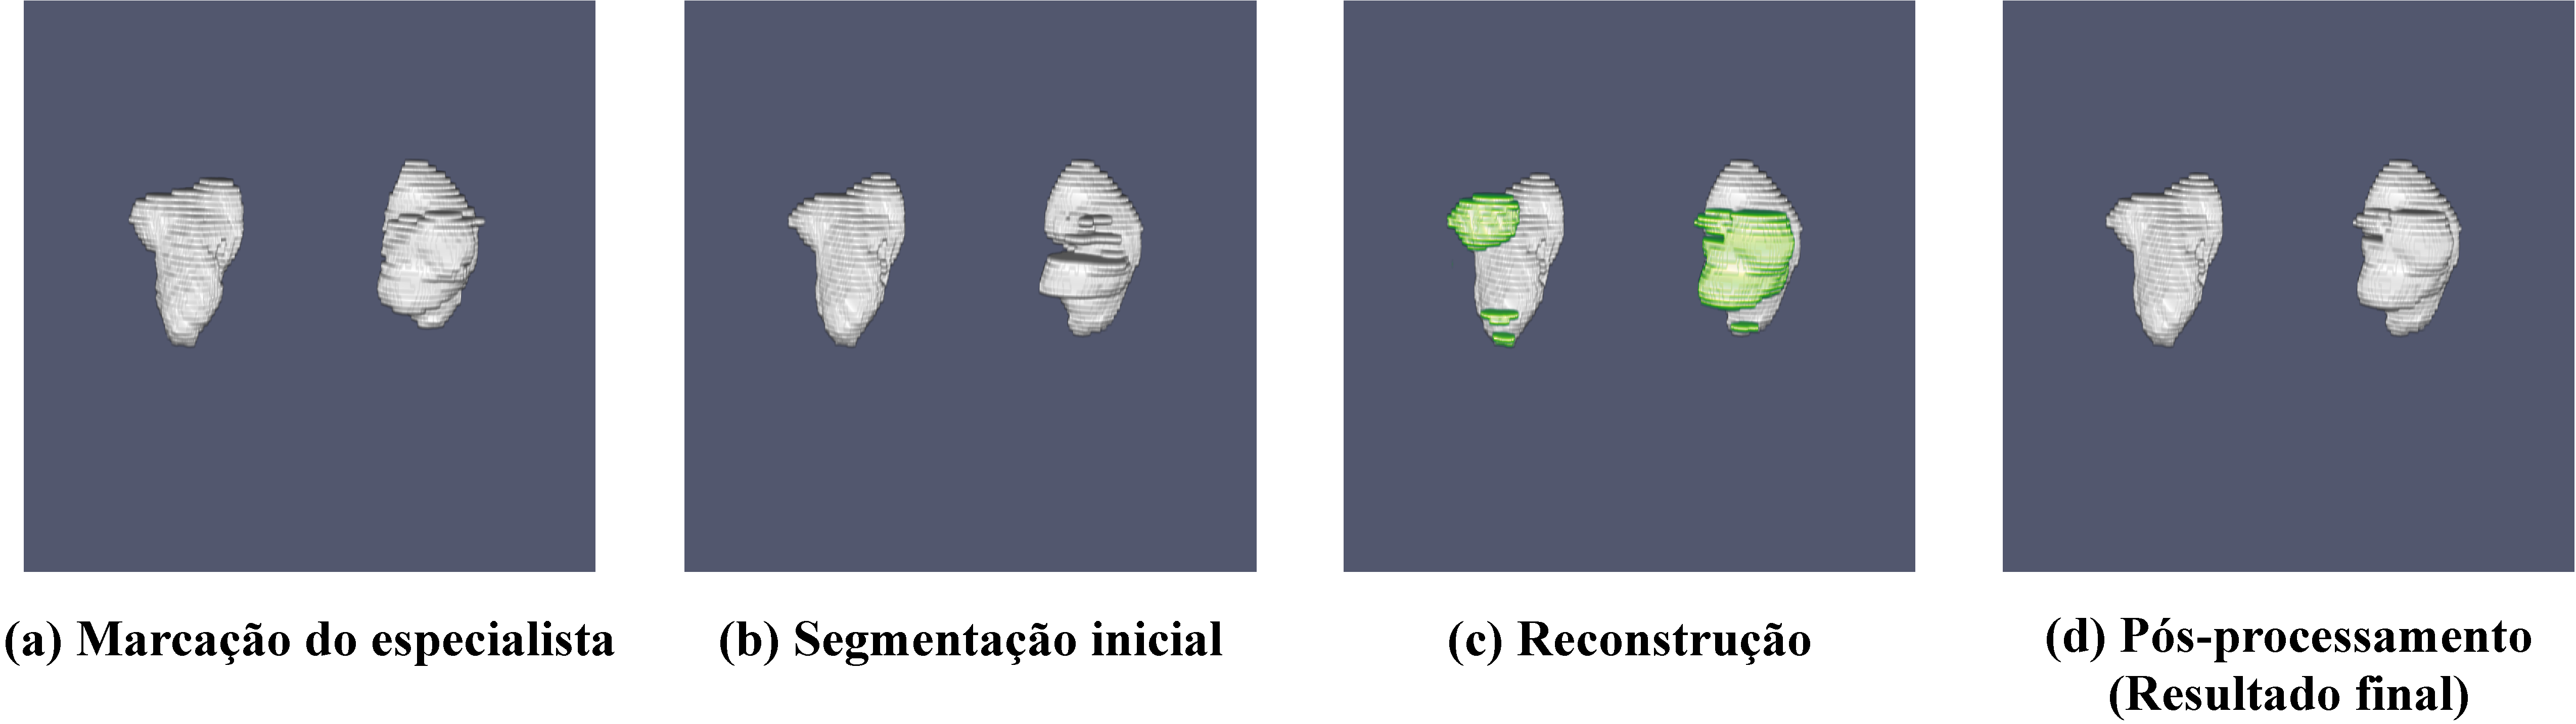
\includegraphics[width=1\textwidth]{figuras/estudos-casos-rins-3-45.pdf}
    \label{fig:estudo-rins-3}
    \legend{Fonte: Elaborado pela autora.}
\end{figure}

\section{Estudos de Caso – Segmentação de Tumores Renais}
\label{sec:estudos-segmentacao-tumores-renais}

Nesta seção, são mostradas e discutidas as situações mais comuns observadas na aplicação das etapas do método proposto para a segmentação de tumores. Os cenários encontrados foram os seguintes: (1) as etapas de reconstrução de tumores renais e pós-processamento afetaram a qualidade da segmentação inicial dos candidatos a tumores renais na região renal; e (2) as etapas de reconstrução de tumores renais e pós-processamento melhoraram a segmentação inicial dos candidatos a tumores renais na região renal.

\subsection{Estudo de Caso 1 – Paciente case\_00012}
\label{sec:estudo-tumores-caso-1}

O primeiro estudo de caso explora uma circunstância em que as etapas de reconstrução e pós-processamento dos tumores afetaram a segmentação inicial de candidatos a tumores renais na região renal. Observa-se na Figura~\ref{fig:estudo-tumores-1} a entrada da rede de segmentação (segmentação final dos rins), a marcação do especialista (b) e as etapas do método proposto (c) e (d). Após as duas últimas etapas (Figura~\ref{fig:estudo-tumores-1} (d)), houve uma deterioração no desempenho em comparação com a segmentação inicial. Neste caso, os resultados finais foram 89,85\% de Dice, 81,57\% de Jaccard, 99,92\% de acurácia 98,71\% de sensibilidade e 99,92\% especificidade. No entanto, a segmentação inicial atingiu 90,69\%, 82,97\%, 99,92\%, 98,04\% e 99,93\% de Dice, Jaccard, acurácia, sensibilidade e especificidade, respectivamente. Dessa forma, as etapas de reconstrução e pós-processamento dos tumores não foram capazes de definir com maior precisão as regiões dos tumores. Este cenário foi observado em 4 pacientes.

%Apesar disso, as taxas de desempenho para a maioria das métricas não mudaram significativamente.

\begin{figure}[!ht]
    \centering
    \caption{Estudo de caso 1. Segmentação dos rins (cinza), segmentação dos tumores renais (vermelho) e reconstrução dos tumores renais (verde).}
    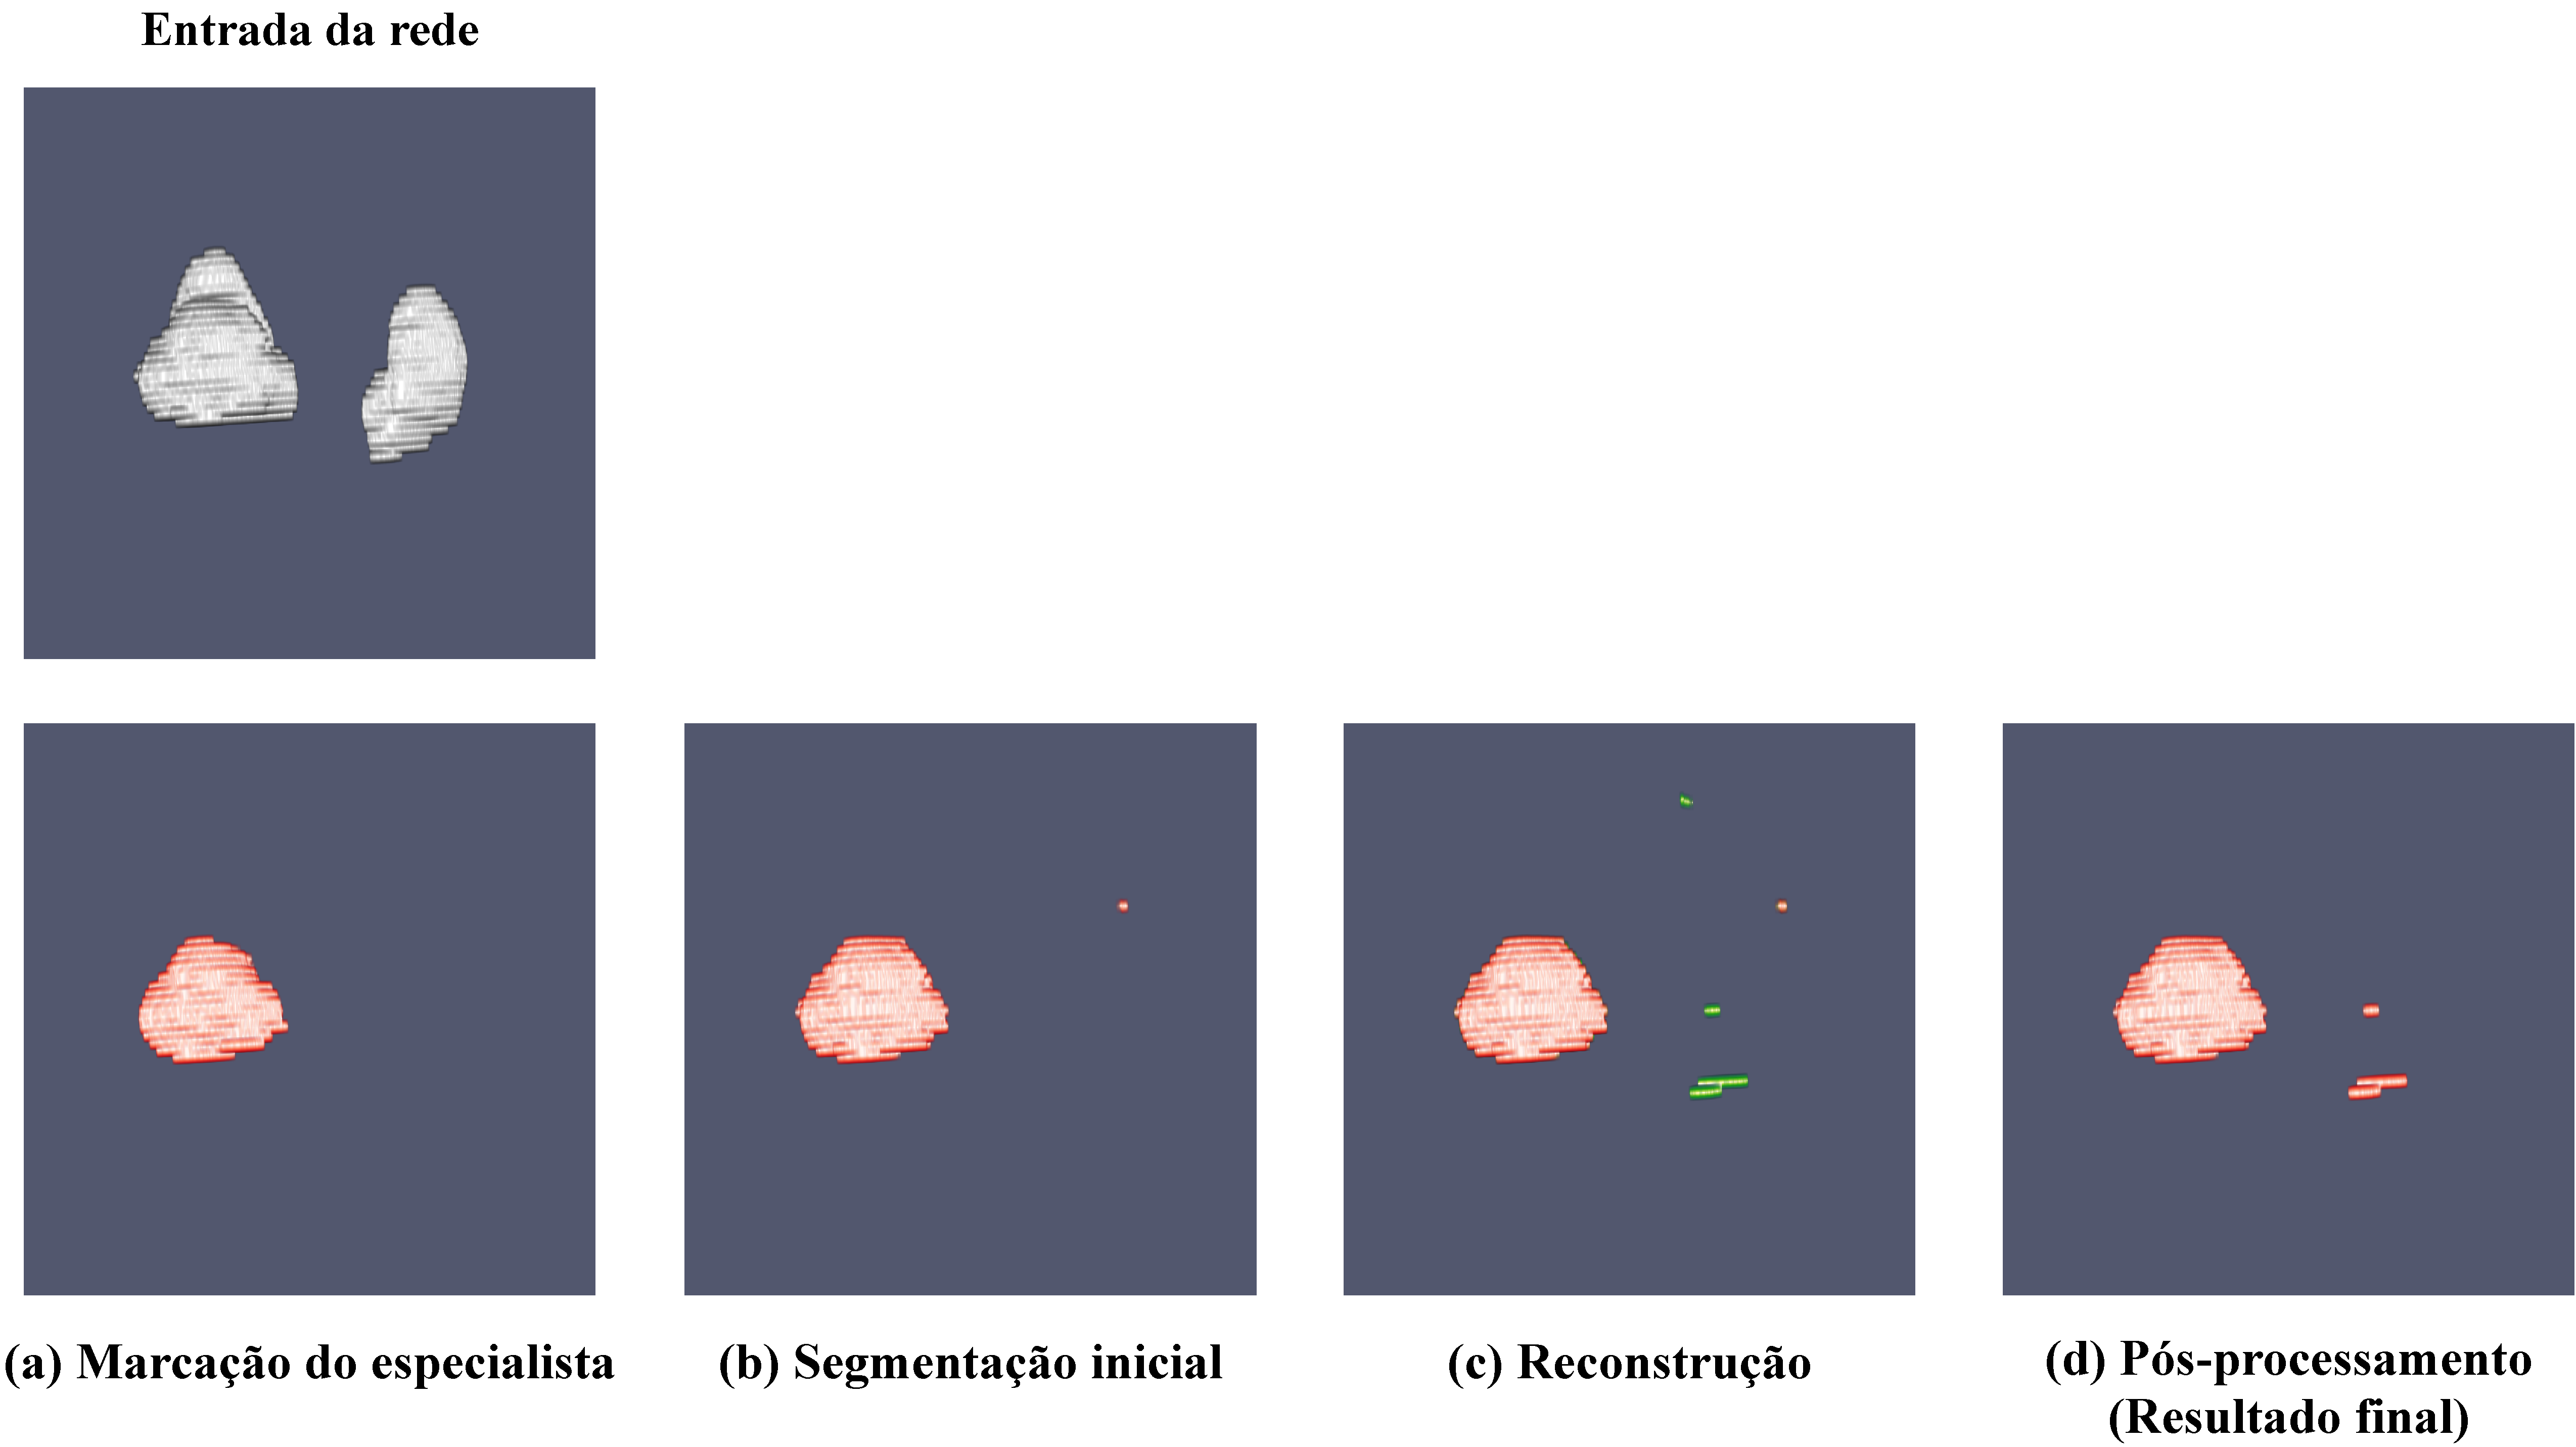
\includegraphics[width=1\textwidth]{figuras/estudos-casos-tumores-renais-1-12.pdf}
    \label{fig:estudo-tumores-1}
    \legend{Fonte: Elaborado pela autora.}
\end{figure}

\subsection{Estudo de Caso 2 – Paciente case\_00028}
\label{sec:estudo-tumores-caso-2}

Neste estudo de caso, as etapas de reconstrução e pós-processamento dos tumores compensaram algumas deficiências da segmentação inicial. Na Figura~\ref{fig:estudo-tumores-2} (b), observa-se que a segmentação inicial gerou vários fragmentos errôneos. Porém, após as etapas de reconstrução e pós-processamento (Figura~\ref{fig:estudo-tumores-2} (c) e Figura~\ref{fig:estudo-tumores-2} (d), respectivamente), a segmentação pelo método proposto eliminou um grande número de falsos positivos. Neste caso, foram obtidos 94,50\% de Dice, 89,57\% Jaccard, 99,97\% de acurácia, 93,85\% de sensibilidade e 99,98\% de especificidade na segmentação final, basicamente uma melhoria significativa de 27,67\% na métrica Dice em comparação com a segmentação inicial, onde os resultados foram 66,83\% de Dice, 50,18\% de Jaccard, 99,84\% de acurácia, 51,52\% de sensibilidade e 99,99\% de especificidade. Este cenário foi observado em 27 casos de teste.

\begin{figure}[!ht]
    \centering
    \caption{Estudo de caso 2. Segmentação dos rins (cinza), segmentação dos tumores renais (vermelho) e reconstrução dos tumores renais (verde).}
    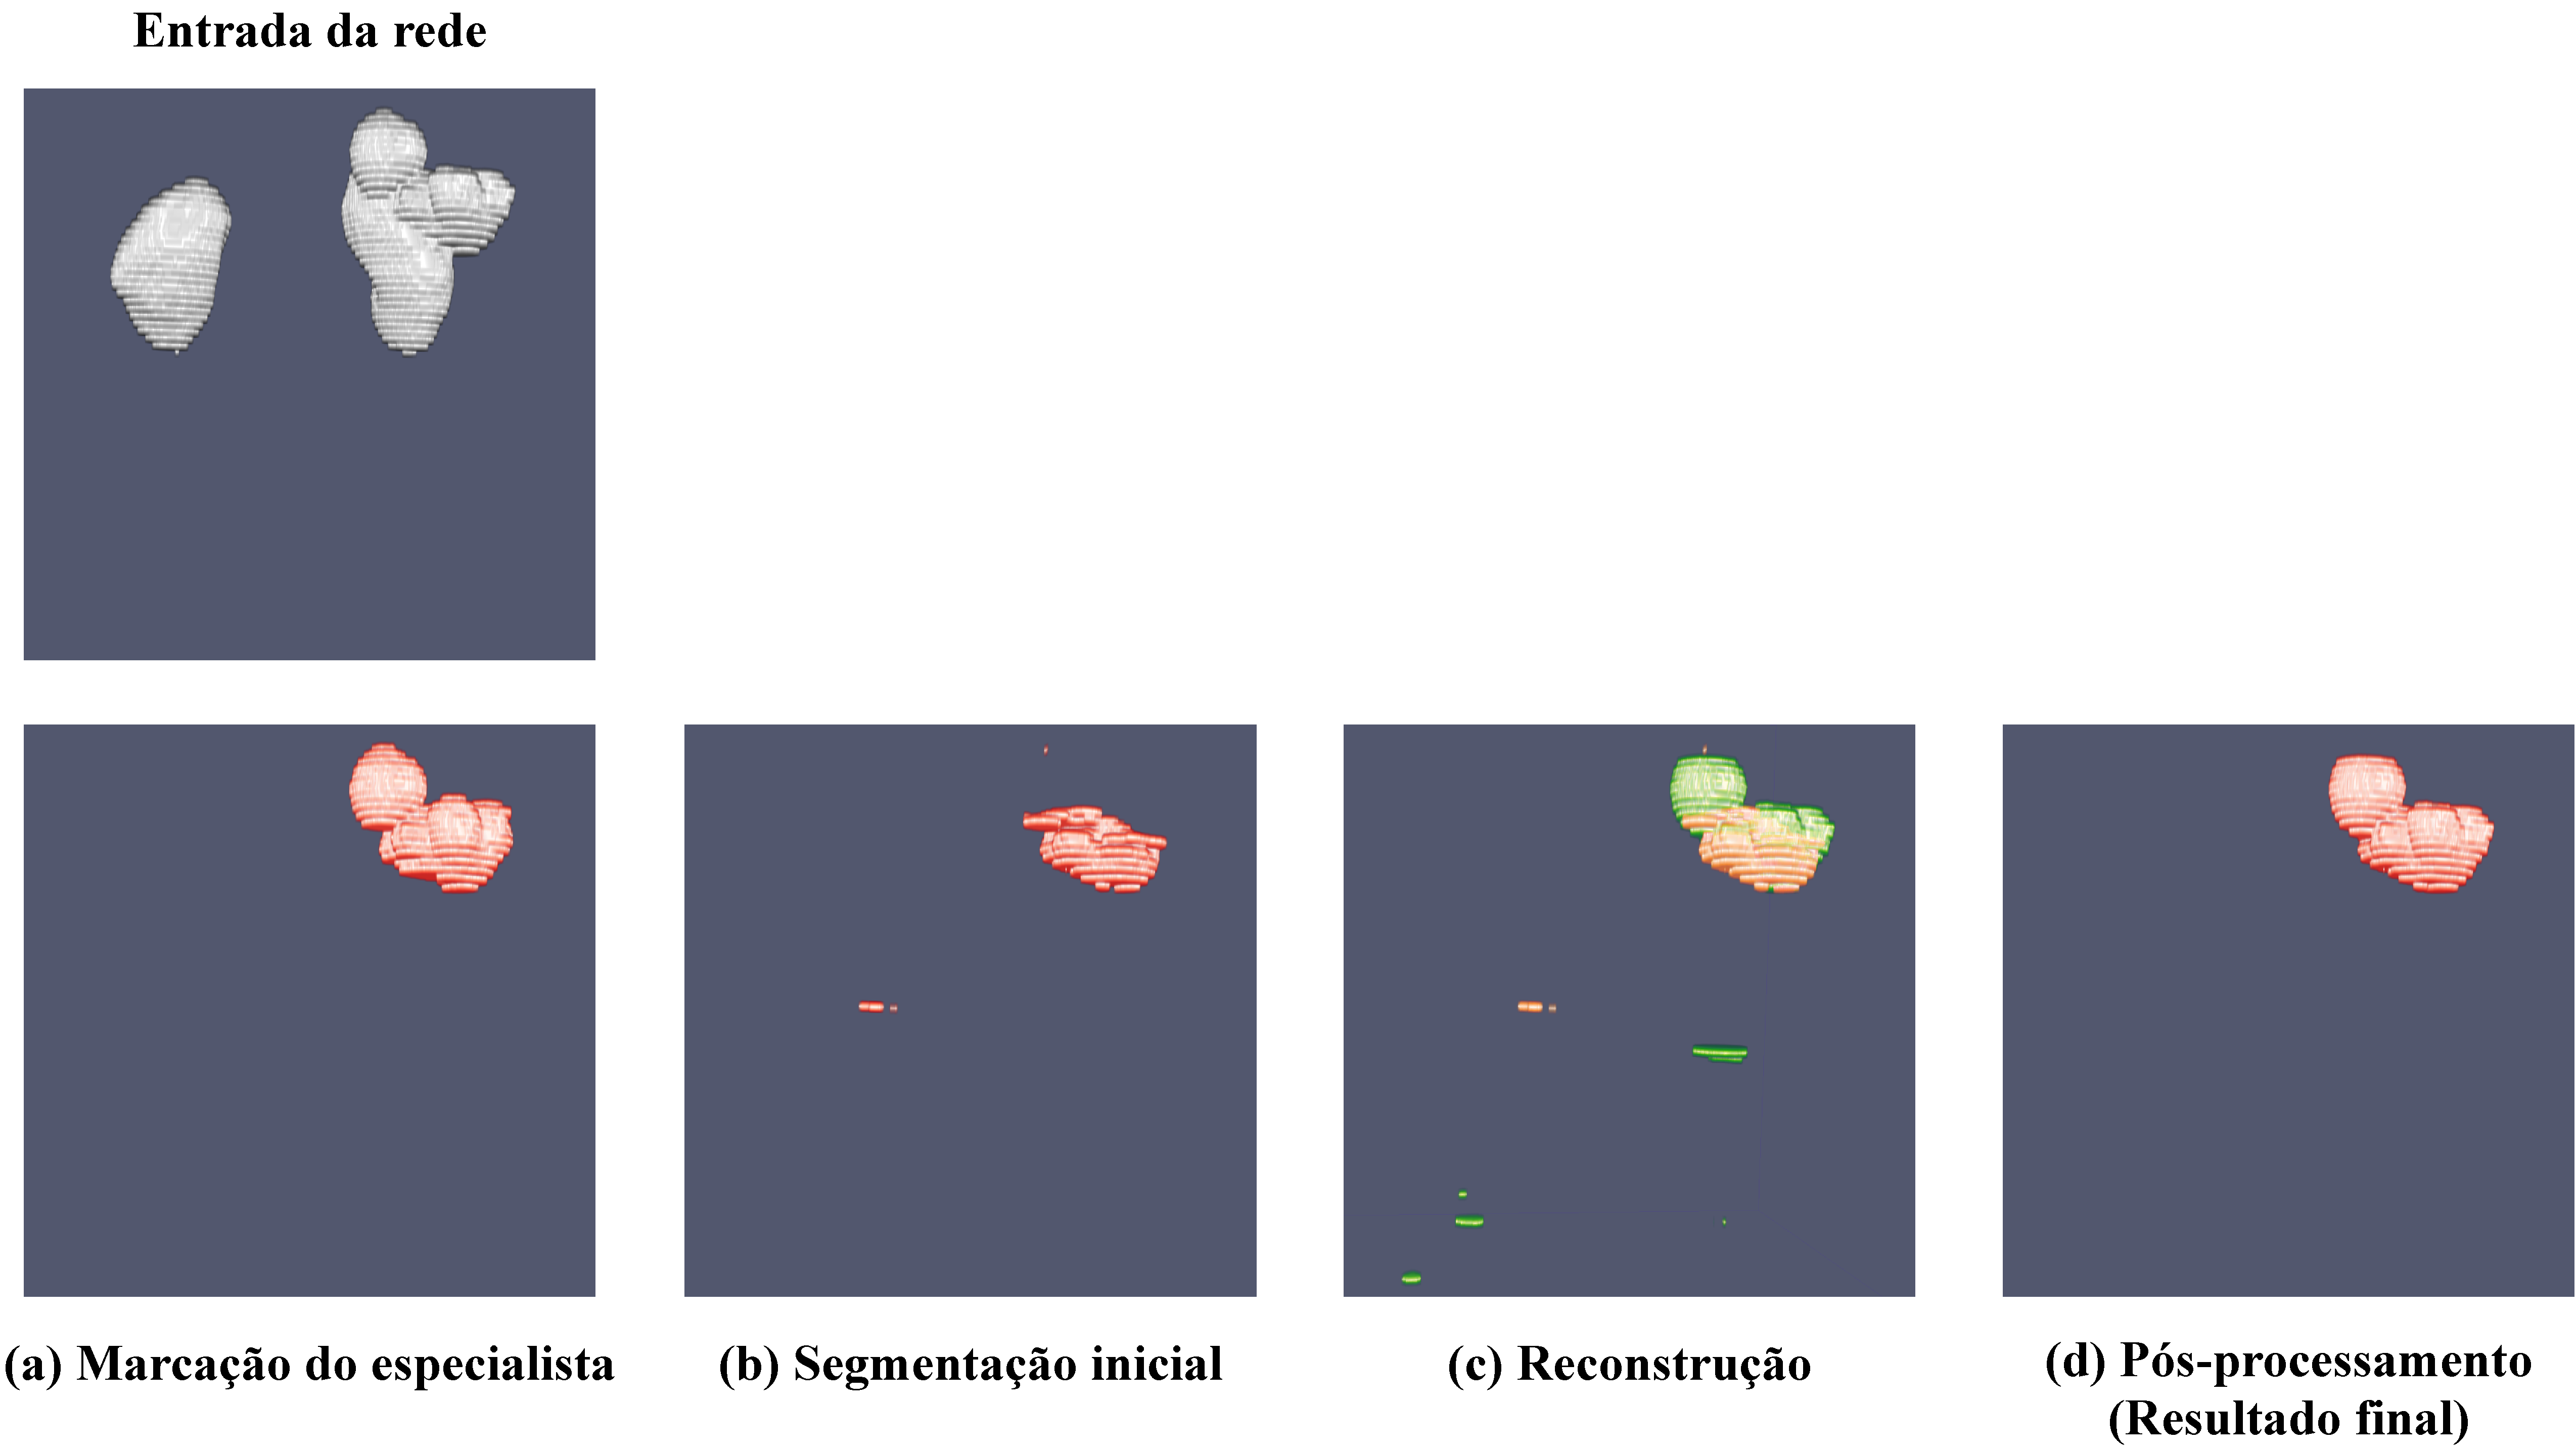
\includegraphics[width=1\textwidth]{figuras/estudos-casos-tumores-renais-2-28.pdf}
    \label{fig:estudo-tumores-2}
    \legend{Fonte: Elaborado pela autora.}
\end{figure}

%\subsection{Estudo de Caso 3 – Vários Pacientes}
%\label{sec:estudo-tumores-caso-3}

%Neste último cenário, pretende-se mostrar que o método proposto é eficiente mesmo quando não há tumores renais em um rim. Esse cenário é ilustrado na Figura~\ref{} na qual são mostrados vários pacientes que tem esse comportamento. Por meio da marcação do especialista (imagem superior) é possível observar que há tumores renais em apenas um rim. Na imagem central da Figura~\ref{}  é obtida a segmentação inicial dos rins (cinza) e candidatos a tumores renais na região renal (vermelho), na qual pode-se observar que os tumores renais foram segmentados apenas no rim que realmente possui tumores. Conforme ilustrado, percebe-se que após a aplicação das etapas de reconstrução dos tumores renais e pós-processamento (imagem inferior), o método proposto permanece consistente e continua melhorando os resultados dos rins e das regiões que apresentam tumores renais. Portanto, conclui-se que o método proposto funciona bem mesmo quando não há tumores renais nos rins. Isso prova que o método pode ser usado mesmo em cenários em que não há tumores renais para segmentar.

\section{Comparação do Método Proposto com os Trabalhos Relacionados}
\label{sec:comparacao}

Nesta seção é apresentada uma análise comparativa dos resultados obtidos pelo método proposto em relação aos trabalhos relacionados (Capítulo~\ref{cap:trabalhos-relacionados}). As subseções a seguir apresentam uma comparação com os trabalhos relacionados à segmentação de rins, segmentação de tumores, e segmentação de rins e tumores renais.

\subsection{Segmentação de Rins}
\label{sec:disc-trab-relac-rins}

Esta subseção mostra os resultados dos trabalhos relacionados à segmentação de rins. A Tabela~\ref{tab:res-trabalhos-relacionados-rins} apresenta um resumo desta comparação, fornecendo informações das técnicas, quantidade de pacientes e as métricas de desempenho usadas em seus métodos. Por fim, são apresentados os resultados do método proposto. 

\begin{table}[!ht]
\caption{Comparação dos resultados do método com trabalhos relacionados à segmentação de rins.}
\label{tab:res-trabalhos-relacionados-rins}
\centering
%\setstretch{1.3}
\doublespacing
\resizebox{\columnwidth}{!}{
\begin{tabular}{p{11cm}ccccccc}
\hline
\centering \textbf{Técnica(s)}                                                                                                       & \textbf{Base} & \textbf{Pacientes} & \textbf{Dice (\%)} & \textbf{Jacc (\%)} & \textbf{Acc (\%)} & \textbf{Sen (\%)} & \textbf{Esp (\%)} \\ \hline
Modelo deformável baseado em \textit{Level Set} \cite{khalifa2011new}                                                     & Privada       & 29                 & 95                 & -                  & 96,36             & 93,8              & -                 \\
Esquema hierárquico de registro e ponderação de atlas \cite{wolz2013automated}                                            & Privada       & 150                & 92,5               & 86,8               & -                 & 98,3              & -                 \\
Continuidade contextual na sequência de imagens de TC \cite{Zhao2013ContextualIK}                                         & Privada       & 10                 & 94,7               & -                  & -                 & -                 & -                 \\
Registro de imagens multi-atlas \cite{yang2014automatic}                                                                  & Privada       & 14 fatias          & 95,2               & -                  & -                 & -                 & -                 \\
Estrutura híbrida baseada de modelos geométricos deformáveis e NMF \cite{khalifa2016kidney}                               & Privada       & 36                 & 96,45              & -                  & -                 & -                 & -                 \\
Contorno ativo usando a estrutura \textit{Level Set} \cite{skalski2017kidney}                                             & Privada       & 10                 & 86,2               & -                  & -                 & -                 & -                 \\
CNNs 3D \cite{jackson2018deep}                                                                                            & Privada       & 113                & 88,5               & -                  & -                 & -                 & -                 \\
Crowdsourcing e CNN \cite{mehta2019segmenting}                                                                            & Privada       & 42                 & 93,2               & -                  & -                 & -                 & -                 \\
U-Net, \textit{patch} e sistema de rastreamento \cite{9534007}                                                            & KiTS19        & 270                & 90,63              & -                  & -                 & -                 & -                 \\ \hline
\textbf{Método proposto com ResUNet 2.5D, DeepLabv3+ 2.5D, agrupador de tumores e técnicas para remover falsos positivos} & KiTS19        & 210                & 97,45              & 95,05              & 99,95             & 98,44             & 99,96             \\ \hline
\end{tabular}
}
\end{table}

Nos últimos anos, muitas técnicas de segmentação renal foram desenvolvidas e aplicadas em diversos estudos. Por exemplo,  \citeonline{khalifa2011new} usaram modelos deformáveis baseados em conjuntos de níveis geométricos para segmentação renal em TC. \citeonline{khalifa2016kidney} também fizeram uso de modelos deformáveis. Os modelos deformáveis são controlados por informações sobre a intensidade e a forma estatística dos rins. Em casos de ruído, imagens de baixa resolução e limites difusos, pode aumentar a instabilidade quanto à identificação dos contornos renais e resultar em falhas no método. \citeonline{khalifa2011new} atingiram um Dice de 95\%, acurácia de 96,36\% e sensibilidade de 93,8\%, considerando apenas 29 pacientes. Em \citeonline{khalifa2016kidney} 95\% de Dice foram alcançados, considerando 36 pacientes. Os dois estudos fazem uso de TCs de pacientes saudáveis, ou seja, sem presença de tumores ou cistos. O método proposto nesta tese usa TCs de pacientes com presença de anormalidades, o que dificulta a segmentação dos rins. Ainda assim, este método superou os resultados dos dois trabalhos descritos.

Alguns trabalhos que usaram atlas e registros foram propostos por \citeonline{wolz2013automated} e \citeonline{yang2014automatic} alcançando métricas promissoras na tarefa de segmentação renal. A desvantagem de suas abordagens é que geralmente elas tem um certo tamanho para resolver o problema em um conjunto de imagens e, ao testar novas imagens de tamanhos diferentes do atlas, o método não tem garantia de funcionar. Observe que em \citeonline{wolz2013automated} o conjunto de imagens usado para validar o método contém 150 pacientes saudáveis e em \citeonline{yang2014automatic} apenas 14 fatias são usadas, das quais seis resultados de segmentação renal com grandes tumores foram excluídos porque o tumor alterou significativamente a forma do rim. O método aqui proposto não usa atlas e registros, o que o torna mais robusto na tarefa de segmentação renal. Além disso, todas as imagens de TC disponíveis na base de imagens foram utilizadas, independentemente dos resultados. O índice de Dice alcançado em nosso método proposto foi de 97,45\%.

O método proposto por \citeonline{Zhao2013ContextualIK} faz uso da continuidade contextual de fatias adjacentes em imagens de TC, então uma estrutura de segmentação baseada em fatias é construída para segmentar automaticamente os rins. Para este propósito, quatro parâmetros contextuais, incluindo distância e sobreposição, são selecionados para estimar a continuidade entre fatias adjacentes. Para isso, utilizam-se algoritmos convencionais de segmentação e modificação (modelo deformável tradicional e limiar iterativo local), chegando a 94,7\% de Dice, utilizando um banco de dados privado composto por 10 pacientes com doenças renais. No método em estudo, propõe-se o uso de duas redes neurais convolucionais para atingir uma segmentação precisa para os rins, assim, são inseridas abordagens capazes de segmentar sem a necessidade de um ponto de partida.

A segmentação dos rins baseada no método Contorno Ativo usando uma estrutura \textit{Level Set} com restrições elipsoidais foi proposta em \citeonline{skalski2017kidney}. A solução proposta leva em consideração as informações sobre a região e os termos de contorno, bem como as restrições dedicadas à característica de formato do rim, o que torna o método bastante restrito e, não é garantido que o método funcione bem com o surgimento de novas imagens com formatos ligeiramente diferentes. O método foi testado em 10 tomografias de pacientes com câncer renal, obtendo resultados de 86,2\% de Dice. Em nossa proposta não há necessidade de informações anatômicas, e alcançou resultados superiores a 97\% de Dice usando 31 pacientes com tumores. \citeonline{jackson2018deep} desenvolveram uma ferramenta automatizada com base em CNNs 3D e alcançaram 88,5\% de Dice usando 113 TCs e \textit{data augmentation offline}.

Em \citeonline{mehta2019segmenting}, os autores usaram uma rede neural convolucional e uma ferramenta de \textit{crowdsourcing} para segmentação de órgãos em larga escala. As validações foram realizadas comparando as segmentações de \textit{crowdsourcing} e segmentações marcadas por especialistas, e verificou que o desempenho não foi significativamente diferente. Porém, a realização de marcações renais por usuários sem o conhecimento especializado na área é imprudente, pois isso pode ser feita de forma errada e afetar a segmentação dos rins e, consequentemente, gerar resultados errados. Os resultados foram 93,2\% de Dice usando para validar uma base de 42 pacientes saudáveis. \citeonline{9534007} apresentaram um método composto por duas etapas. Na primeira etapa, é realizada a segmentação semântica baseada na rede U-Net e \textit{batch}. Na segunda etapa, um sistema de rastreamento (\textit{middle-bottom, middle-top}) foi usado para encontrar contornos do rim nas fatias de TC restantes. O método desenvolvido atingiu um Dice de 90,63\%.

\subsection{Segmentação de Tumores Renais}
\label{sec:disc-trab-relac-tumor-renal}

Esta segunda subseção apresentada uma análise comparativa do método proposto com os trabalhos relacionados à segmentação de tumores renais. O resumo desses trabalhos é apresentado na Tabela~\ref{tab:res-trabalhos-relacionados-tumor-renal}, com informações sobre as técnicas usadas, quantidade de pacientes e as métricas de desempenho aplicadas. Além disso, a última linha da tabela apresenta os resultados obtidos pelo método proposto neste estudo.

\begin{table}[!ht]
\caption{Comparação dos resultados do método com trabalhos relacionados à segmentação de tumores renais.}
\label{tab:res-trabalhos-relacionados-tumor-renal}
\centering
%\setstretch{1.3}
\doublespacing
\resizebox{\columnwidth}{!}{
\begin{tabular}{p{11cm}ccccccc}
\hline
\centering \textbf{Técnica(s)}                                                                                                       & \textbf{Base} & \textbf{Pacientes} & \textbf{Dice(\%)} & \textbf{Jacc(\%)} & \textbf{Acc(\%)} & \textbf{Sen(\%)} & \textbf{Esp(\%)} \\ \hline
Estrutura hibrida baseada em SIFCM e DRLSE \cite{kaur2019hybrid}                                                          & Privada       & 40                 & 88,2              & 88,5              & 86,51            & -                & -                \\
CNNs fracamente supervisionada \cite{yang2020weakly}                                                                      & Privada       & 200                & 82,6              & -                 & -                & -                & -                \\
MB-FSGAN \cite{RUAN2020101721}                                                                                            & Privada       & 113                & 85,9              & -                 & 95,7             & 86,2             & 89,4             \\
HybridNet 3D \cite{Yan9098325}                                                                                            & KiTS19        & 300                & 79,7              & -                 & -                & -                & -                \\
V-Net usando \textit{Two-Stage Bottleneck Block} \cite{turk2022kidney}                                                    & KiTS19        & 210                & 86,9              & 76,8              & -                & -                & -                \\
3D U-Net preservando a simetria rotacional em cortes axiais \cite{Tanimoto22}                                             & Privada       & 213                & 60,4              & -                 & -                & -                & -                \\ \hline
\textbf{Método proposto com ResUNet 2.5D, DeepLabv3+ 2.5D, agrupador de tumores e técnicas para remover falsos positivos} & KiTS19        & 210                & 84,06             & 75,04             & 99,94            & 88,33            & 99,95            \\ \hline
\end{tabular}
}
\end{table}

É importante mencionar que todos os trabalhos relacionados nesta subseção desenvolveram métodos semiautomáticos que segmentam os tumores a partir da marcação dos rins feita por especialistas. Isso torna o método dependente do especialista humano, pois não houve uma etapa para segmentação dos rins por técnicas computacionais. \citeonline{kaur2019hybrid} sugerem uma técnica de segmentação híbrida baseada em dois métodos que incluem SIFCM (\textit{Spatial Intuitionistic Fuzzy C-Means Clustering}) que integra detalhes de imagem espacial e DRLSE (\textit{Distance Regularized Level-Sets Evolution}) para extração de lesão renal. Esta abordagem requer uma estimativa grosseira da região de interesse fornecida pelo SIFCM dentro do rim. Assim, o resultado correto da segmentação depende das informações preliminares e da posição da função de definição de nível. Portanto, a inicialização adequada do ajuste de nível próximo ao limite do tumor renal é essencial para a demarcação correta. O método foi validado em 40 TCs de pacientes com câncer renal, obtendo resultados de 88,2\% Dice, 88,5\% Jaccard e acurácia de 86,51\%. Em nosso método foram testados mais exames, e não há necessidade de aproximar a região de interesse, além disso, não foram usadas marcações dos rins feitas por especialistas, mas sim por técnica computacional.

\citeonline{yang2020weakly} usaram um conjunto de CNNs fracamente supervisionada para segmentação de tumores. Uma estrutura de três estágios foi introduzida para treinar as CNNs com as anotações fracas de tumores (caixas delimitadoras). Para treinamento das CNNs, cada imagem é aplicada \textit{data augmentation offline}, totalizando 14.400 novas imagens. O resultado do trabalho foi de 82,6\% de Dice usando TCs de 200 pacientes. Nosso método obteve resultados acima de 82\% de Dice. Além disso, foi utilizado \textit{data augmentation} em tempo real, o que apresenta um método com melhor desempenho e baixo consumo de recursos de máquina.

No estudo de \citeonline{RUAN2020101721} é proposto o MB-FSGAN, que consiste em um extrator de características em várias escalas, e alcançaram 85,9\% de Dice, 95,7\% de acurácia, 86,2\% de sensibilidade e 89,4\% de especificidade, usando 113 TCs. Neste estudo, levaram em consideração apenas 20 pacientes para testar o método. No estudo recente de \citeonline{Tanimoto22}, um modelo U-Net 3D foi usado para segmentar tumores levando em consideração a estrutura global dos rins. O método obteve resultados promissores de 60,4\% de Dice utilizando 213 TCs.

Trabalhos como os de \citeonline{Yan9098325, turk2022kidney} também usaram abordagens 3D para segmentar tumores. Esses métodos apresentam desempenho superior a 79,7\% de Dice, consumindo alto poder computacional. Vale ressaltar que essas abordagens que usam como entrada regiões renais completas, podem apresentar resultados mais expressivos, já que para segmentar os tumores usam as marcações manuais dos rins feitas por especialistas. Em nosso estudo, foram alcançados 84,06\% de Dice para os tumores usando uma abordagem completa (segmentação dos rins e tumores) com baixo custo computacional comparado aos trabalhos citados.

\subsection{Segmentação de Rins e Tumores Renais}
\label{sec:disc-trab-relac-rins-tumor-renal}

Nesta última subseção, são apresentados os trabalhos relacionados a segmentação de rins e tumores renais. Na Tabela~\ref{tab:res-trabalhos-relacionados-rins-tumor-renal} é apresentado o resumo dos trabalhos relacionados, da mesma forma que nas subseções anteriores, no qual contém as informações sobre as técnicas aplicadas, quantidade de pacientes e as métricas de desempenho. Os resultados para rins são expostos na linha superior e os tumores renais na linha inferior. Finalmente, são mostrados os resultados obtidos pelo método proposto.

\begin{table}[!ht]
\caption{Comparação dos resultados do método proposto com os trabalhos relacionados à segmentação de rins e tumores renais.}
\label{tab:res-trabalhos-relacionados-rins-tumor-renal}
\centering
%\setstretch{1.3}
\doublespacing
\resizebox{\columnwidth}{!}{
\begin{tabular}{p{11cm}ccccccc}
\hline
\centering \textbf{Técnica(s)}                                                                                                       & \textbf{Base}                                              & \textbf{Pacientes} & \textbf{Dice(\%)}                                     & \textbf{Jacc(\%)}                                     & \textbf{Acc(\%)}                                      & \textbf{Sen(\%)}                                      & \textbf{Esp(\%)}                                      \\ \hline
Rede 3D com PPM + Atlas \cite{yang2018automatic}                                                                          & Privada                                                    & 140                & \begin{tabular}[c]{@{}c@{}}93,1\\ 80,2\end{tabular}   & -                                                     & -                                                     & -                                                     & -                                                     \\
Modelo hibrido V-Net \cite{turk2020kidney}                                                                                & KiTS19                                                     & 210                & \begin{tabular}[c]{@{}c@{}}97,7\\ 86,5\end{tabular}   & -                                                     & -                                                     & -                                                     & -                                                     \\
Rede residual híbrida 3D com SE \cite{QAYYUM2020104097}                                                                   & KiTS19                                                     & 210                & \begin{tabular}[c]{@{}c@{}}97,8\\ 86,8\end{tabular}   & -                                                     & -                                                     & \begin{tabular}[c]{@{}c@{}}95,6\\ 91,31\end{tabular}  & \begin{tabular}[c]{@{}c@{}}99,6\\ 91,45\end{tabular}  \\
SE-ResNeXT U-Net \cite{seru2020}                                                                                          & KiTS19                                                     & 300                & \begin{tabular}[c]{@{}c@{}}96,77\\ 74,32\end{tabular} & -                                                     & -                                                     & -                                                     & -                                                     \\
MSS U-Net 3D \cite{ZHAO2020100357}                                                                                        & KiTS19                                                     & 210                & \begin{tabular}[c]{@{}c@{}}96,9\\ 80,5\end{tabular}   & -                                                     & -                                                     & -                                                     & -                                                     \\
\textit{Attention} U-Net \cite{9708025}                                                                                            & KiTS19                                                     & 205                & \begin{tabular}[c]{@{}c@{}}95,65\\ 93,86\end{tabular} & -                                                     & -                                                     & -                                                     & -                                                     \\
U-Nets 3D: simples, residual e residual de pré-ativação \cite{HELLER2021101821}                                           & KiTS19                                                     & 210                & \begin{tabular}[c]{@{}c@{}}97,4\\ 85,1\end{tabular}   & -                                                     & -                                                     & -                                                     & -                                                     \\
3D U-Net \cite{Lin2021}                                                                                                   & Privada                                                    & 441                & \begin{tabular}[c]{@{}c@{}}97,3\\ 84,4\end{tabular}   & -                                                     & -                                                     & -                                                     & -                                                     \\
3D-MS-RFCNN \cite{YANG2022106616}                                                                                         & \begin{tabular}[c]{@{}c@{}}KiTS19 +\\ Privada\end{tabular} & 480                & \begin{tabular}[c]{@{}c@{}}91,62\\ 71,64\end{tabular} & -                                                     & -                                                     & -                                                     & -                                                     \\
3D-CNN e ConvLSTM \cite{KANG2022103334}                                                                                   & KiTS19                                                     & 300                & \begin{tabular}[c]{@{}c@{}}96,39\\ 78,9\end{tabular}  & -                                                     & -                                                     & -                                                     & -                                                     \\ \hline
\textbf{Método proposto com ResUNet 2.5D, DeepLabv3+ 2.5D, agrupador de tumores e técnicas para remover falsos positivos} & KiTS19                                                     & 210                & \begin{tabular}[c]{@{}c@{}}97,45\\ 84,06\end{tabular} & \begin{tabular}[c]{@{}c@{}}95,05\\ 75,04\end{tabular} & \begin{tabular}[c]{@{}c@{}}99,95\\ 99,94\end{tabular} & \begin{tabular}[c]{@{}c@{}}98,44\\ 88,33\end{tabular} & \begin{tabular}[c]{@{}c@{}}99,96\\ 99,95\end{tabular} \\ \hline
\end{tabular}
}
\end{table}

Vale mencionar que nesta subseção são considerados os trabalhos que fazem o processo completo, segmentando os rins e tumores automaticamente. Esses trabalhos são propostos por \citeonline{yang2018automatic, turk2020kidney, QAYYUM2020104097, seru2020, ZHAO2020100357, 9708025, HELLER2021101821, Lin2021,YANG2022106616, KANG2022103334}. \citeonline{turk2020kidney} apresentam um novo modelo híbrido usando recursos aprimorados em modelos V-Net existentes. Usando um conjunto de 20 TCs para testar o modelo, alcançaram resultados de 97,7\% e 86,8\% de Dice para os rins e tumores, respectivamente. Em nosso estudo, obtivemos resultados semelhantes usando um conjunto de 31 TCs para teste.

Nos trabalhos de \citeonline{seru2020} e \citeonline{9708025} foram feita combinações de arquiteturas. \citeonline{seru2020} combinaram as vantagens da SE-Net, ResNeXT e U-Net, e obtiveram 96,77\% e 74,32\% de Dice para rins e tumores, respectivamente. \citeonline{9708025} implementaram um modelo U-Net com camadas \textit{Attention Gate}, alcançando em seu método um Dice de 95,65\% para rins e 93,86\% para tumores, usando 20 TCs para teste. Em nosso estudo, também realizamos combinações de arquiteturas, como a DeepLabv3+ ajustada com o codificador DPN-131, e obtivemos resultados semelhantes, 97,45\% de Dice para rins e 84,06\% para tumores usando 31 TCs para teste.

Finalmente, são apresentados vários outros trabalhos que usaram aprendizado profundo para segmentar os rins e tumores. Esses métodos apresentaram resultados bem-sucedidos e se destacaram pela arquitetura 3D, que apresenta alto desempenho, como no trabalho de \citeonline{QAYYUM2020104097} que propuseram uma rede residual 3D híbrida com \textit{Squeeze-and-Excitation} (SE). A rede foi treinada em 4.000 épocas, com alto poder de processamento. Foram obtidos resultados de 97,8\% de Dice para rins e 86,8\% de Dice para tumores, usando uma base de imagens de 210 pacientes, dentre eles, 10\% para testar o método. \citeonline{ZHAO2020100357} implementaram uma U-Net 3D supervisionada em várias escalas, MSS U-Net 3D U-Net, e também tiveram um bom desempenho, alcançando um Dice de 96,9\% e 80,5\% para rins e tumores, respectivamente.

No estudo de \citeonline{KANG2022103334} é proposta uma rede combinando as caracterísitcas da ConvLSTM e U-Net 3D e são obtidos resultados expressivos de 96,39\% de Dice para rins e 78,9\% para tumores. \citeonline{Lin2021} construíram dois modelos de segmentação 3D baseados em U-Net. No trabalho de \citeonline{YANG2022106616} propuseram uma nova rede neural profunda, a 3D-MS-RFCNN para melhorar a segmentação em tumores de tamanho extremamente grande. Ambos os trabalhos tiveram bons desempenhos para segmentação de rins e tumores, usando base de imagens extensas, porém privadas. Isso acaba limitando a realização de experimentos com essas bases de imagens.

\citeonline{HELLER2021101821} e \citeonline{yang2018automatic} também propuseram abordagens 3D. \citeonline{HELLER2021101821} usaram três modelos 3D da UNet e alcançaram o primeiro lugar no desafio KiTS19. Para treinar a rede usaram 1.000 épocas. Além disso, os autores afirmam que não mostraram nenhum benefício significativo na construção do modelo. O poder da abordagem 3D foi suficiente para alcançar os melhores resultados, no entanto, alto poder computacional é consumido. Essa abordagem atingiu 97,4\% de Dice para rins e 85,1\% de Dice para os tumores. \citeonline{yang2018automatic} apresentaram um método que usa redes 3D combinadas com PPM e atlas. Além disso, foi aplicado o \textit{data augmentation offline}, gerando 90.000 novas imagens, cerca de 1.000 vezes mais que o número de imagens originais. Como resultado, obtiveram 93,1\% e 80,2\% de Dice para rins e tumores, respectivamente, usando 140 TCs. Nosso método obteve excelente desempenho nas segmentações dos rins e tumores em comparação aos modelos 3D existentes com baixo custo computacional.

De acordo com as Tabelas~\ref{tab:res-trabalhos-relacionados-rins},~\ref{tab:res-trabalhos-relacionados-tumor-renal} e~\ref{tab:res-trabalhos-relacionados-rins-tumor-renal}, pode-se observar que existem vários métodos na literatura que investigam a segmentação dos rins e tumores. Além disso, as técnicas se tornaram cada vez mais robustas ao longo dos anos e quase sempre alcançaram um desempenho superior a 86\% e 80\% em todas as métricas de validação para segmentação de rins e tumores, respectivamente. Ademais, é possível verificar que os melhores resultados fazem uso de abordagens 3D em seu método. As técnicas de aprendizado profundo são promissoras, mas apresentam várias desvantagens, como o alto custo computacional e grande quantidade de conjunto de imagens necessário. Portanto, as abordagens 3D nem sempre são opções viáveis.

Em contraste com os métodos descritos na literatura, destaca-se que o trabalho proposto usa modelos de última geração em conjunto com abordagens 2.5D de baixo custo computacional. Esses modelos são capazes de segmentar rins e tumores com alta precisão, garantindo melhor os limites (bordas) dos objetos e removendo o máximo de previsões erradas. Isso diminui o trabalho do médico especialista em verificar todas as regiões consideradas rins e tumores. Além disso, o método proposto obteve resultados comparáveis aos trabalhos da literatura, mostrando-se promissor e robusto. Por fim, vale ressaltar que diversas métricas são utilizadas para validar o método proposto, ao contrário dos trabalhos relacionados, o que impossibilitam outras comparações. Dessa forma, é possível demonstrar a viabilidade da utilização do método proposto para segmentação de rins e tumores em TC.

\section{Aspectos Importantes do Método Proposto}
\label{sec:aspectos-importantes}

A segmentação de rins e tumores em exames tomográficos não é uma tarefa trivial. Desenvolver um método capaz de contornar todas as adversidades desses órgãos e atingir uma boa taxa de acerto ainda é um desafio. Nesta tese, as principais etapas de um sistema CAD (aquisição de imagens, pré-processamento, segmentação e pós-processamento) foram aplicadas. O método se mostrou robusto e preciso na segmentação de rins e tumores. Ressalta-se a importância dos aspectos e limitações encontrados após a análise das etapas propostas.

\begin{enumerate}
    \item O estudo em questão é um método completo para resolver o problema de segmentação dos rins e tumores. Nesta área de pesquisa, a dificuldade desta tarefa é amplamente reconhecida. Por esse motivo, os resultados obtidos ganham lugar de destaque entre os métodos de última geração encontrados na literatura.
    
    \item Tendo conhecimento sobre a anatomia dos rins e tumores renais, sabe-se que podem ser heterogêneos em suas características (forma e textura). Dessa forma, é possível ver a importância de uma etapa adicional para encontrar padrões de características existentes e agrupar os casos (exames) semelhantes de acordo com os padrões identificados. Com a formação dos grupos de tumores e distribuindo-os proporcionalmente entre o conjunto de treinamento e validação, garantiu-se que os modelos ficassem equilibrados e tivessem melhor desempenho, pois existem diferentes tipos de tumores nos conjuntos de treinamento e validação. Essa etapa foi fundamental para o sucesso das demais etapas.
    
    \item Em relação ao uso de aumento de dados em tempo real, é uma técnica de regularização implícita para combater o \textit{overfitting} de modelos de aprendizado profundo \cite{kukavcka2017regularization}. O que não foi diferente nesse estudo, a combinação das operações aplicadas em tempo de execução obteve uma maior diversidade dos tumores renais no conjunto de treinamento, resultando em um maior poder de generalização. Consequentemente, houve um impacto positivo nas métricas de validação para segmentação dos tumores. Esses aumentos mostram que é uma abordagem poderosa para melhorar a generalização e robustez de modelos usando baixo consumo de recursos de máquina.
    
    \item O método proposto é um processo automatizado executado por dois modelos CNN, que são ferramentas muito robustas que realizam implicitamente a extração e seleção de características. Este é um aspecto positivo, pois elimina a necessidade de extrair empiricamente o conjunto de características a serem utilizadas no processo de aprendizagem e de definir as técnicas a serem usadas na seleção das características.
    
    \item Outro aspecto importante foi o uso da abordagem 2.5D. Uma das vantagens dessa abordagem é que as informações espaciais de fatias vizinhas são usadas para identificar tumores, sem comprometer a complexidade computacional. Isso aumentou as chances de segmentação bem-sucedida e reduziu os falsos positivos. Além disso, foi feito um balanceamento das fatias de rins e tumores. Isso contribuiu para que a rede também aprendesse as fatias sem rins/tumores, o que ajudou a reduzir ainda mais os falsos positivos, que é um dos maiores desafio.
    
    \item É importante notar que a etapa inicial de segmentação do rim por si só foi capaz de fornecer bons resultados, comparáveis a outros estudos relevantes na literatura. Acredita-se que isso tenha sido possível devido ao desempenho robusto da arquitetura ResUNet, visto que as informações sobre as camadas são propagadas com a abordagem residual, mantendo e agregando características renais relevantes, o que consequentemente resultou em melhores resultados.
    
    \item Para segmentar os candidatos a tumores na região renal, foi usado o modelo DeepLabv3+ 2.5D com o codificador DPN-131. Esse codificador compartilha as vantagens de redes robustas (ResNet e DenseNet) \cite{chen2017dual} e ao combinar com a DeepLabv3+ 2.5D, permitiu a exploração de novos recursos, possibilitando o aprendizado de representações tumorais a partir da captura de suas informações contextuais, como diferentes formas e tamanhos. Além disso, o decodificador DeepLabv3+ recupera gradualmente as informações espaciais para reconstruir a saída, capturando melhor os limites dos objetos \cite{chen2018encoder}. Essa combinação resultou em uma rede codificador-decodificador eficiente com alto desempenho para segmentação de candidatos a tumores.
    
    \item Ademais, para segmentar os candidatos a tumores renais na região renal, uma abordagem em cascata é aplicada. Essa abordagem consiste em usar os resultados da segmentação dos rins como entrada para segmentar os tumores. Esse processo reduz o escopo do problema e os erros de segmentação inicial dos tumores. No entanto, pode acontecer de regiões que não foram segmentadas nos rins sejam possíveis regiões tumorais. Caso isso aconteça, não é possível predizer essas regiões e isso acaba reduzindo a chance de obter melhores resultados. Pensando nisso, incluiu-se a etapa de segmentar os candidatos a tumores renais na região abdominal, o que ocasionou melhor segmentação, pois foram recuperadas partes das regiões tumorais.
    
    \item A aplicação da etapa de reconstrução dos tumores renais foi capaz de unir porções consideráveis das regiões tumorais, melhorando os resultados da segmentação dos tumores e também dos rins. Isso foi possível porque à medida que as regiões tumorais foram recuperadas, as regiões renais também foram, pois as regiões tumorais fazem parte dos rins. Portanto, a reconstrução dos tumores renais também possibilitou melhorar a segmentação dos rins.
    
    \item Com a etapa de reconstrução dos tumores renais, vários falsos positivos foram adicionados. Entretanto, ao selecionar apenas os dois maiores elementos na etapa de pós-processamento dos rins, foi possível eliminar não só os falsos positivos encontrados na segmentação inicial, mas também na reconstrução dos tumores renais. Esse pós-processamento acabou impactando positivamente no resultado final da segmentação dos rins e tumores.
    
    \item Na etapa de pós-processamento dos tumores renais, os elementos segmentados com informações contextuais insuficientes para representar os tumores foram removidos, preservando-se apenas os elementos contínuos. Assim, o pós-processamento melhorou a precisão da segmentação dos tumores, removendo muitos falsos positivos. Essa etapa resultou em uma melhoria considerável na maioria dos casos.
    
    \item Finalmente, a combinação de todas as técnicas neste estudo proporcionou uma melhor segmentação dos rins e tumores. Até onde sabe-se, este é o primeiro método que combinou explicitamente todas essas técnicas. Comparado com trabalhos relacionados, o método proposto apresentou resultados expressivos e ganhou destaque, alcançando na segmentação de rins um Dice de 97,45\%, Jaccard de 95,05\%, acurácia de 99,95\%, sensibilidade de 98,44\% e especificidade de 99,96\%. E na segmentação dos tumores atingiu 84,06\%, 75,04\%, 99,94\%, 88,33\% e 99,95\% de Dice, Jaccard, acurácia, sensibilidade e especificidade, respectivamente.
\end{enumerate}

Embora o método proposto apresente vários fatores positivos, também apresenta algumas limitações, nas quais destacam-se:

\begin{enumerate}
    \item A segmentação dos rins e tumores é promissora e significativa, sendo comparável a trabalhos relevantes da literatura. No entanto, a abordagem 2.5D é limitada em termos espaciais do volume de TC. Acredita-se que para obter um melhor desempenho é necessário explorar recursos 3D. Entretanto, não foram explorados devido às limitações de consumo de \textit{hardware} e memória.
    
    \item Com a etapa de reconstrução dos tumores renais, muitas regiões de rins e tumores que não foram segmentadas acabaram sendo recuperadas. Entretanto, algumas regiões não foram totalmente recuperadas. Portanto, outra técnica (por exemplo, \textit{ensemble}) poderia ser adicionada para segmentar mais regiões tumorais, a fim de melhorar a sensibilidade.
    
    \item Por fim, vale destacar que o pós-processamento usado na segmentação de rins e tumores apresenta deficiências, em que ora o pós-processamento contribui efetivamente para a remoção de falsos positivos e ora afeta a segmentação. Portanto, é importante explorar novas técnicas de pós-processamento que sejam mais estáveis para a etapa de remoção de falsos positivos.
\end{enumerate}

Os aspectos positivos discutidos nas etapas do método proposto contribuíram para que os resultados obtidos fossem comparáveis aos trabalhos encontrados na literatura. É perceptível que existem diversos métodos na literatura que propõem soluções para o problema da segmentação dos rins e tumores utilizando abordagens 3D. No entanto, essas abordagens requerem um alto custo/esforço computacional. O método proposto, apesar de algumas limitações, foi capaz de obter resultados satisfatórios com baixo custo computacional. Portanto, este estudo apresenta contribuições para o meio científico e é de fundamental importância na demarcação dos rins e tumores pelo especialista, contribuindo para aumentar a produtividade e melhorar os índices diagnósticos.


\chapter{Conclusão}
\label{cap:conclusao}
\phantom{2}

As altas taxas de incidência do câncer de rim em todo o mundo mostram a importância do desenvolvimento de pesquisas que forneçam suporte ao diagnóstico precoce da doença. Essa é uma etapa fundamental para viabilizar o tratamento adequado aos pacientes. Nesse contexto, este trabalho apresentou um método automático para a tarefa de segmentação de rins e tumores renais baseado em aprendizado profundo e técnicas de processamento de imagens para reduzir os falsos positivos.

O método proposto apresenta quatro etapas principais. Na primeira etapa, utiliza técnicas de processamento de imagens, como realce da imagem e normalização das intensidades do \textit{voxel}. Além de aplicar técnicas para agrupar tumores renais a fim de distribuir proporcionalmente o conjunto de treinamento e validação. Na segunda etapa, as segmentações iniciais de rins e tumores são obtidas usando ResUNet 2.5D e DeepLabv3+ 2.5D, respectivamente. Na terceira etapa, a reconstrução dos tumores renais usa outro modelo ResUNet 2.5D. Finalmente, na quarta etapa, as segmentações finais dos rins e tumores renais são obtidas por meio do pós-processamento para remoção de elementos que não fazem parte dos rins e tumores.

Para validar o método proposto, foi usada a base de imagem pública KiTS19. Essa base de imagens consiste em tomografias de pacientes em diferentes estágios da doença, tornando-a altamente heterogênea e complexa. Dessa forma, a segmentação dos rins e tumores é uma tarefa desafiadora em cenários realistas. Os resultados experimentais revelaram um desempenho promissor para a tarefa proposta, atingindo 97,47\% de Dice, 95,09\% de Jaccard, 99,95\% de acurácia, 97,86\% de sensibilidade e 99,97\% de especificidade para segmentação de rins. Para a segmentação de tumores foi obtido 82,94\% de Dice, 72,54\% de Jaccard, 99,95\% de acurácia, 86,51\% de sensibilidade e 99,96\% de especificidade. De maneira geral, os resultados fornecem fortes evidências de que o método proposto é uma ferramenta poderosa que pode ser incorporada aos sistemas CAD para auxiliar no diagnóstico da doença.

\section{Contribuições}
\label{sec:contribuições}

As principais contribuições do método proposto nesta tese são descritas a seguir:

\begin{enumerate}
    \item Desenvolvimento de um método automático para agrupar casos (exames) e distribuí-los proporcionalmente no conjunto de treinamento e validação para garantir que os modelos fossem equilibrados e obtivessem melhor desempenho;
    
    \item Adaptação da arquitetura DeepLabv3+, com o uso da DPN-31 como codificador para a segmentação de tumores renais, fornecendo resultados precisos;
    
    \item Aplicação da técnica de balanceamento de fatias nos conjuntos de treinamento e validação juntamente com a abordagem 2.5D, contribuindo para reduzir consideravelmente os falsos positivos e detectando se uma fatia apresenta rins/tumores ou não;
    
    \item A aplicação da etapa de reconstrução de tumores renais por meio da combinação de duas CNNs recuperou partes consideráveis de regiões de tumores e, consequentemente, proporcionou melhores resultados de segmentação renal;
    
    \item Aplicação de técnicas de processamento de imagens baseadas em informações contextuais para reduzir falsos positivos em segmentações de rins e tumores.
\end{enumerate}

\section{Trabalhos Futuros}
\label{sec:trabalhos-futuros}

Apesar dos bons resultados obtidos para a segmentação de rins e tumores renais em imagens de TCs, melhorias ainda podem ser feitas no método proposto visando incrementar a sua eficiência. A seguir são destacadas algumas sugestões:

\begin{enumerate}
    \item Considerando a diversidade de aquisições da base de imagens, padronizar as entradas da rede usando uma rede \textit{autoencoder} como um pré-processamento poderia aumentar a eficiência dos modelos de segmentação;
    
    \item Assim como na abordagem 2.5D usada no método proposto, as fatias são visualizadas sequencialmente. Acredita-se que o uso de recursos recorrentes da rede neural pode melhorar o desempenho, pois essas redes podem “lembrar” informações de fatias anteriores, adicionando recursos ao modelo;
    
    \item Aprimorar ou construir um \textit{ensemble} na etapa de reconstrução dos tumores renais a fim de melhorar a sensibilidade;
    
    \item Construir um método para fazer uma triagem de TCs com e sem tumores renais. Este novo método seria integrado ao método proposto como uma etapa inicial para identificar quais TCs têm tumores renais. Posteriormente, TCs com tumores seriam usadas como entrada para segmentar as regiões com tumores.
    
    %\item Outra técnica de pós-processamento, como o fechamento morfológico, poderia ser incrementada para aumentar os objetos segmentados e recuperar mais regiões de rins e tumores renais, e assim melhorar os resultados obtidos;
\end{enumerate}

\section{Produções Científicas}
\label{sec:producoes-cientificas}

A Tabela~\ref{tab:artigos-autoria} apresenta os artigos diretamente relacionados ao método proposto para a segmentação de rins e tumores renais em imagens de TC. Além disso, a Tabela~\ref{tab:artigos-coautoria} lista os artigos científicos publicados e submetidos em outras aplicações de processamento de imagens e visão computacional desde o início do doutorado.

\begin{table}[ht!]
\centering
\caption{Produções científicas em relação ao método proposto para segmentação de rins e tumores renais.}
\label{tab:artigos-autoria}
\resizebox{\columnwidth}{!}{
\begin{tabular}{p{10cm}lccc}
\hline
\textbf{Artigo}                                                                                                                         & \centering \textbf{Tipo} & \textbf{Qualis} & \textbf{Status} \\ \hline
Kidney Segmentation from Computed Tomography Images using Deep Neural Network. Em: Computers in Biology and Medicine. Ano: 2020.        & Periódico     & A1              & Publicado       \\ \hline
Kidney Tumor Segmentation from Computed Tomography Images using DeepLabv3+ 2.5D Model. Em: Expert Systems with Applications. Ano: 2021. & Periódico     & A1              & Publicado      \\ \hline
\end{tabular}
}
\end{table}

\begin{table}[ht!]
\centering
\caption{Produções científicas em outras aplicações de processamento de imagens e visão computacional.}
\label{tab:artigos-coautoria}
\resizebox{\columnwidth}{!}{
\begin{tabular}{p{11cm}lccc}
\hline
\textbf{Artigo}                                                                                                                                                                            & \textbf{Tipo} & \textbf{Qualis} & \textbf{Status} \\ \hline
Interferometer Eye Image Classification for Dry Eye Categorization using Phylogenetic Diversity Indexes for Texture Analysis. Em: Computer Methods and Programs in Biomedicine. Ano: 2019. & Periódico     & A1              & Publicado       \\ \hline
Tear Film Classification in Interferometry Eye Images using Phylogenetic Diversity Indexes and Ripley's K Function. Em: IEEE Journal of Biomedical and Health Informatics. Ano: 2020.      & Periódico     & A1              & Publicado       \\ \hline
Planejamento Cirúrgico de Estrabismo Horizontal Utilizando Árvore de Regressão de Múltiplas Saídas. Em: Simpósio Brasileiro de Computação Aplicada à Saúde. Ano: 2020.                     & Simpósio      & B3              & Publicado       \\ \hline
An Automatic Method for Segmentation of Liver Lesions in Computed Tomography Images Using Deep Neural Networks. Em: Expert Systems with Applications. Ano: 2021.                           & Periódico     & A1              & Publicado       \\ \hline
Surgical Planning of Horizontal Strabismus Using Multiple Output Regression Tree. Em: Computers in Biology and Medicine. Ano: 2021.                                                        & Periódico     & A1              & Publicado       \\ \hline
Automatic Method for Classifying COVID-19 Patients Based on Chest X-ray Images, using Deep Features and PSO-optimized XGBoost. Em: Expert Systems with Applications. Ano: 2021.            & Periódico     & A1              & Publicado       \\ \hline
Segmentation and Quantification of COVID-19 Infections in CT using Pulmonary Vessels Extraction and Deep Learning. Em: Multimedia Tools and Applications. Ano: 2021.                       & Periódico     & A2              & Publicado       \\ \hline
Classificação Automática de Glóbulos Brancos usando Descritores de Forma e Textura e eXtreme Gradient Boosting. Em: Simpósio Brasileiro de Computação Aplicada à Saúde. Ano: 2020.         & Simpósio      & B3              & Publicado       \\ \hline
Liver Segmentation from Computed Tomography Images using Cascade Deep Learning. Em: Computers in Biology and Medicine. Ano: 2021.                                                           & Periódico     & A1              & Publicado       \\ \hline
Heart Segmentation in Planning CT using 2.5D U-Net++ with Attention Gate. Em: Computer Methods in Biomechanics and Biomedical Engineering: Imaging \& Visualization. Ano: 2021.            & Periódico     & A3              & Publicado       \\ \hline
\end{tabular}
}
\end{table}

% \include{proposta de marcador_natural}
% related works - proposta - resultados
% \include{cap4_estimacao_pose}
% related works - proposta - resultados
% \include{cap5_panoramas_aumentados}
% related works - proposta - resultados
% \chapter{Conclusão}
\label{cap:conclusao}
\phantom{2}

As altas taxas de incidência do câncer de rim em todo o mundo mostram a importância do desenvolvimento de pesquisas que forneçam suporte ao diagnóstico precoce da doença. Essa é uma etapa fundamental para viabilizar o tratamento adequado aos pacientes. Nesse contexto, este trabalho apresentou um método automático para a tarefa de segmentação de rins e tumores renais baseado em aprendizado profundo e técnicas de processamento de imagens para reduzir os falsos positivos.

O método proposto apresenta quatro etapas principais. Na primeira etapa, utiliza técnicas de processamento de imagens, como realce da imagem e normalização das intensidades do \textit{voxel}. Além de aplicar técnicas para agrupar tumores renais a fim de distribuir proporcionalmente o conjunto de treinamento e validação. Na segunda etapa, as segmentações iniciais de rins e tumores são obtidas usando ResUNet 2.5D e DeepLabv3+ 2.5D, respectivamente. Na terceira etapa, a reconstrução dos tumores renais usa outro modelo ResUNet 2.5D. Finalmente, na quarta etapa, as segmentações finais dos rins e tumores renais são obtidas por meio do pós-processamento para remoção de elementos que não fazem parte dos rins e tumores.

Para validar o método proposto, foi usada a base de imagem pública KiTS19. Essa base de imagens consiste em tomografias de pacientes em diferentes estágios da doença, tornando-a altamente heterogênea e complexa. Dessa forma, a segmentação dos rins e tumores é uma tarefa desafiadora em cenários realistas. Os resultados experimentais revelaram um desempenho promissor para a tarefa proposta, atingindo 97,47\% de Dice, 95,09\% de Jaccard, 99,95\% de acurácia, 97,86\% de sensibilidade e 99,97\% de especificidade para segmentação de rins. Para a segmentação de tumores foi obtido 82,94\% de Dice, 72,54\% de Jaccard, 99,95\% de acurácia, 86,51\% de sensibilidade e 99,96\% de especificidade. De maneira geral, os resultados fornecem fortes evidências de que o método proposto é uma ferramenta poderosa que pode ser incorporada aos sistemas CAD para auxiliar no diagnóstico da doença.

\section{Contribuições}
\label{sec:contribuições}

As principais contribuições do método proposto nesta tese são descritas a seguir:

\begin{enumerate}
    \item Desenvolvimento de um método automático para agrupar casos (exames) e distribuí-los proporcionalmente no conjunto de treinamento e validação para garantir que os modelos fossem equilibrados e obtivessem melhor desempenho;
    
    \item Adaptação da arquitetura DeepLabv3+, com o uso da DPN-31 como codificador para a segmentação de tumores renais, fornecendo resultados precisos;
    
    \item Aplicação da técnica de balanceamento de fatias nos conjuntos de treinamento e validação juntamente com a abordagem 2.5D, contribuindo para reduzir consideravelmente os falsos positivos e detectando se uma fatia apresenta rins/tumores ou não;
    
    \item A aplicação da etapa de reconstrução de tumores renais por meio da combinação de duas CNNs recuperou partes consideráveis de regiões de tumores e, consequentemente, proporcionou melhores resultados de segmentação renal;
    
    \item Aplicação de técnicas de processamento de imagens baseadas em informações contextuais para reduzir falsos positivos em segmentações de rins e tumores.
\end{enumerate}

\section{Trabalhos Futuros}
\label{sec:trabalhos-futuros}

Apesar dos bons resultados obtidos para a segmentação de rins e tumores renais em imagens de TCs, melhorias ainda podem ser feitas no método proposto visando incrementar a sua eficiência. A seguir são destacadas algumas sugestões:

\begin{enumerate}
    \item Considerando a diversidade de aquisições da base de imagens, padronizar as entradas da rede usando uma rede \textit{autoencoder} como um pré-processamento poderia aumentar a eficiência dos modelos de segmentação;
    
    \item Assim como na abordagem 2.5D usada no método proposto, as fatias são visualizadas sequencialmente. Acredita-se que o uso de recursos recorrentes da rede neural pode melhorar o desempenho, pois essas redes podem “lembrar” informações de fatias anteriores, adicionando recursos ao modelo;
    
    \item Aprimorar ou construir um \textit{ensemble} na etapa de reconstrução dos tumores renais a fim de melhorar a sensibilidade;
    
    \item Construir um método para fazer uma triagem de TCs com e sem tumores renais. Este novo método seria integrado ao método proposto como uma etapa inicial para identificar quais TCs têm tumores renais. Posteriormente, TCs com tumores seriam usadas como entrada para segmentar as regiões com tumores.
    
    %\item Outra técnica de pós-processamento, como o fechamento morfológico, poderia ser incrementada para aumentar os objetos segmentados e recuperar mais regiões de rins e tumores renais, e assim melhorar os resultados obtidos;
\end{enumerate}

\section{Produções Científicas}
\label{sec:producoes-cientificas}

A Tabela~\ref{tab:artigos-autoria} apresenta os artigos diretamente relacionados ao método proposto para a segmentação de rins e tumores renais em imagens de TC. Além disso, a Tabela~\ref{tab:artigos-coautoria} lista os artigos científicos publicados e submetidos em outras aplicações de processamento de imagens e visão computacional desde o início do doutorado.

\begin{table}[ht!]
\centering
\caption{Produções científicas em relação ao método proposto para segmentação de rins e tumores renais.}
\label{tab:artigos-autoria}
\resizebox{\columnwidth}{!}{
\begin{tabular}{p{10cm}lccc}
\hline
\textbf{Artigo}                                                                                                                         & \centering \textbf{Tipo} & \textbf{Qualis} & \textbf{Status} \\ \hline
Kidney Segmentation from Computed Tomography Images using Deep Neural Network. Em: Computers in Biology and Medicine. Ano: 2020.        & Periódico     & A1              & Publicado       \\ \hline
Kidney Tumor Segmentation from Computed Tomography Images using DeepLabv3+ 2.5D Model. Em: Expert Systems with Applications. Ano: 2021. & Periódico     & A1              & Publicado      \\ \hline
\end{tabular}
}
\end{table}

\begin{table}[ht!]
\centering
\caption{Produções científicas em outras aplicações de processamento de imagens e visão computacional.}
\label{tab:artigos-coautoria}
\resizebox{\columnwidth}{!}{
\begin{tabular}{p{11cm}lccc}
\hline
\textbf{Artigo}                                                                                                                                                                            & \textbf{Tipo} & \textbf{Qualis} & \textbf{Status} \\ \hline
Interferometer Eye Image Classification for Dry Eye Categorization using Phylogenetic Diversity Indexes for Texture Analysis. Em: Computer Methods and Programs in Biomedicine. Ano: 2019. & Periódico     & A1              & Publicado       \\ \hline
Tear Film Classification in Interferometry Eye Images using Phylogenetic Diversity Indexes and Ripley's K Function. Em: IEEE Journal of Biomedical and Health Informatics. Ano: 2020.      & Periódico     & A1              & Publicado       \\ \hline
Planejamento Cirúrgico de Estrabismo Horizontal Utilizando Árvore de Regressão de Múltiplas Saídas. Em: Simpósio Brasileiro de Computação Aplicada à Saúde. Ano: 2020.                     & Simpósio      & B3              & Publicado       \\ \hline
An Automatic Method for Segmentation of Liver Lesions in Computed Tomography Images Using Deep Neural Networks. Em: Expert Systems with Applications. Ano: 2021.                           & Periódico     & A1              & Publicado       \\ \hline
Surgical Planning of Horizontal Strabismus Using Multiple Output Regression Tree. Em: Computers in Biology and Medicine. Ano: 2021.                                                        & Periódico     & A1              & Publicado       \\ \hline
Automatic Method for Classifying COVID-19 Patients Based on Chest X-ray Images, using Deep Features and PSO-optimized XGBoost. Em: Expert Systems with Applications. Ano: 2021.            & Periódico     & A1              & Publicado       \\ \hline
Segmentation and Quantification of COVID-19 Infections in CT using Pulmonary Vessels Extraction and Deep Learning. Em: Multimedia Tools and Applications. Ano: 2021.                       & Periódico     & A2              & Publicado       \\ \hline
Classificação Automática de Glóbulos Brancos usando Descritores de Forma e Textura e eXtreme Gradient Boosting. Em: Simpósio Brasileiro de Computação Aplicada à Saúde. Ano: 2020.         & Simpósio      & B3              & Publicado       \\ \hline
Liver Segmentation from Computed Tomography Images using Cascade Deep Learning. Em: Computers in Biology and Medicine. Ano: 2021.                                                           & Periódico     & A1              & Publicado       \\ \hline
Heart Segmentation in Planning CT using 2.5D U-Net++ with Attention Gate. Em: Computer Methods in Biomechanics and Biomedical Engineering: Imaging \& Visualization. Ano: 2021.            & Periódico     & A3              & Publicado       \\ \hline
\end{tabular}
}
\end{table}

\renewcommand{\nomname}{\listadesiglasname\bigskip}
\postextual
  

\bibliography{capitulos/referencias}


%\begin{apendicesenv}

% Imprime uma página indicando o início dos apêndices
%\partapendices

%\begin{KeepFromToc} nao necessario

%\chapter*{APÊNDICE A - Termo de Consentimento Livre e Esclarecido}
%\begin{figure}[!ht]
%\centering
%\includegraphics[scale=0.80]{termo.pdf}
%\end{figure}

%auto_depo

%\chapter*{APÊNDICE B - Termo de Autorização de Depoimento}
%\begin{figure}[!ht]
%\centering
%\includegraphics[scale=0.80]{auto_depo.pdf}
%\end{figure}

%\chapter*{APÊNDICE C - Roteiro de Entrevista}
%\begin{figure}[!ht]
%\centering
%\includegraphics[scale=0.80]{roteiro.pdf}
%\end{figure}

%\end{KeepFromToc} nao necessario

%\end{apendicesenv}

%\begin{anexosenv}

% Imprime uma página indicando o início dos anexos
%\partanexos

%\chapter*{ANEXO A - RESOLUÇÃO Nº 64, DE 05 DE DEZEMBRO DE 2014}
%\begin{figure}[!ht]
%\centering
%\includegraphics[scale=0.80]{res64.pdf}
%\end{figure}

%\includepdf[pages={2-},scale=0.9,pagecommand={}]{res64.pdf}
% \end{anexosenv}

\end{document}
